%% 博士、正常版本、强制使用 Windows 系统字体
\documentclass[lang=chs, degree=phd, blindreview=false, winfonts=true]{yanputhesis}
%%=============================================================================%
%% 导入宏包
%%-----------------------------------------------------------------------------%
\usepackage{listings, listings-rust}    %rust高亮
\usepackage{listings-riscv}             %riscv汇编高亮
\usepackage{underscore}                 %使下划线不需要添加斜线转义
% \usepackage[english]{babel}   %解决label中不能添加下划线问题,但是带来副作用,会把文档语言设置为英文
\usepackage{placeins}                   %解决图片浮动问题
\usepackage{pifont}                     %可以使用带圈数字序号
\usepackage{tabularx}                   %制作更精细的表格
% \usepackage{algorithm}                  %伪代码算法包
% \usepackage{algorithmic}                %伪代码算法包
\usepackage{csquotes}                   %使用\enquote命令,引号
%%=============================================================================%
%% 基本信息录入
%%-----------------------------------------------------------------------------%
\header{NPUcore操作系统内核构建实践}                                             %设置页眉
%%=============================================================================%
%% 文档开始
%%-----------------------------------------------------------------------------%
\begin{document}

\frontmatter                                                                   %前言部分
\makeBookCoverPage{NPUcore操作系统内核构建实践 \\ 基础篇}{NPU_logo.png}          %封面
\setcounter{page}{1}                                                           %设置目录页编号从1开始
\tableofcontents                                                               %目录页

\mainmatter                                                                    %正文部分
\sDefault
\chapter{NPUcore简介(Introduction)}

“NPUcore”是西北工业大学的操作系统内核构建实践型教学操作系统,曾获得2022年OSKernel大赛内核实现赛道一等奖。
NPUcore致力于使用Rust新型编程语言,帮助老师和学生自行研制一个操作系统微型内核,提升操作系统原理的实践体验并探索新型操作系统的设计与实现。
原始的2022版NPUcore具有内存管理、进程管理、文件系统核心系统调用功能,支持RISCV32/64指令集,可在对应的QEMU模拟器和SiFive-U740、K210等嵌入式开发板上运行。
该版本基于rCore-Tutorial迭代开发,重构90\%模块以支持Linux接口,共实现系统调用81个,是一个不错的baseline。
虽然该版本有着不错的性能,但却无法支持全部测例,以及国内自主研发的LoongArch龙芯架构。不仅如此,该版本不支持网络协议,EXT4文件系统,以及其它多种多样的外设,因此我们认为,这个版本仍然有很大的优化空间。
如此,针对初赛和决赛阶段,我们的贡献可以总结为以下四点,并在后文中详细展开:
\begin{enumerate}
    \item 独自实现了2022版本的NPUcore到2k1000平台(龙芯架构)的适配,并封装为一个arch包,方便后人持续开发。
    \item 基本完成了NPUcore在ext4文件系统的适配,但仍有少部分bug。
    \item 调研了几乎所有的开源轻量版ext4仓库,并针对此次适配做了一定总结。
    \item 其它小规模增量:
    \begin{itemize}
        \item 在NPUcore-重生之我是菜狗队伍的指导下,适配了网络模块,并在fat32文件系统上跑出分数。(由于这个增量更多属于另一组,所以我们不会在此次文档中进行大面积介绍)
        \item 独自在ext4文件系统上适配了PCI和SATA驱动,可以从镜像中读取到测例。
        \item 对在2k1000板子上烧录测例进行了初步探索,并总结出了对应的步骤。
    \end{itemize}
\end{enumerate}

% \section{Rust特性}

% Rust是一个“安全、并发、实用”,支持函数式、并发式、过程式以及面向对象的程序设计风格的新型语言。
% Rust在完全公开的情况下开发,并且相当欢迎社区的反馈。近些年,Rust语言在工业应用上的势头越来越猛。
% 基于Rust语言的种种特性,我们认为它更适合一些底层应用的开发,尤其是OSKernel。

% \textbf{1. 我们为什么选择Rust作为OS编程语言?}
% Rust 是一门内存安全的语言。对于 C/C++ 这样的手动管理内存的编程语言,我们在分配堆变量的时候需要调用 malloc/new函数,而当该变量使用完毕之后要手动调用
% free/delete 回收内存。这就要求程序员需要关注所有堆变量的生命周期并及时将其释放,否则就会造成内存泄漏的问题,而过早的释放堆变量又可能造成“use-after-
% free” 的问题。而 Rust 独特的所有权机制和借用检查,让编译器掌管变量的生
% 命周期,使得变量的回收变得可控,同时也杜绝了”use-after-free” 的问题,又不至于带来垃圾回收的开销。

% Rust还能够推断出类型的大小,然后分配正确的内存大小并将其设置为您要求的值。但这意味着无法分配未初始化的内存:Rust没有null的概念。 
% 此外,所有这些检查都是在编译时完成的,因此没有运行时开销,这也是为什么Rust被成为是安全的“C”。 
% 如果你编写了正确的C++代码,你将编写出与C++代码基本上相同的Rust代码。而且由于编译器的帮忙,编写错误的代码版本是不可能的。
% 所以,我们选择Rust语言的原因,不仅是因为他安全,还因为其享有和C一样的速度,和更丰富的库。


% \textbf{2.unsafe关键字}

% 几乎每个语言都有unsafe关键字,但Rust语言使用unsafe的原因可能与其它编程语言还有所不同。接下来我们展示一下unsafe的特性:
% \begin{lstlisting}[language={Rust}, label={code:unsafe},
% 	caption={unsafe展示(r1 是一个裸指针)}]
% fn main() {
%     let mut num = 5;

%     let r1 = &num as *const i32;

%     unsafe {
%         println!("r1 is: {}", *r1);
%     }
% }
% \end{lstlisting}
% 在代码块\ref{code:unsafe}中,r1 是一个裸指针(raw pointer),由于它具有破坏Rust内存安全的潜力,因此只能在unsafe代码块中使用,如果你去掉unsafe\{\},编译器会立刻报错。
% 在我们的NPUcore中,对于一个OS来说,安全是最大的保障,因此unsafe在初期NPUcore建设中给予了很大帮助。因为,即使做到小心谨慎,依然会有出错的可能性,但是 unsafe 语句块决定了:就算内存访问出错了,你也能立刻意识到,错误是在 unsafe 代码块中,而不花大量时间像无头苍蝇一样去寻找问题所在。
% unsafe不安全,但是该用的时候就要用,在一些时候,它能帮助我们大幅降低代码实现的成本。虽然在网上充斥着“千万不要使用 unsafe,因为它不安全”的言论。事实上,我们认为unsafe是一个有效且必要的手段,因此我们选择遵循如下规则去使用:
% \begin{enumerate}
%     \item 没必要用时,就不用;
%     \item 当有必要用时,就大胆用,但是要控制好边界;
%     \item 尽量保证unsafe的边界范围最小。
% \end{enumerate}

\section{NPUcore操作系统}

「NPUcore」是西北工业大学的操作系统内核构建实践型教学操作系统。致力于使用Rust新型编程语言,帮助老师和学生自行研制一个操作系统微型内核,提升操作系统原理的实践体验并探索新型操作系统的设计与实现。目前NPUcore具有内存管理、进程管理、文件系统核心功能,支持RISCV32/64指令集,可在QEMU模拟器和SiFive-U740、K210等嵌入式开发板上运行。

以下为NPUcore的所有的系统调用:

\section{预备知识及技能}
\subsection{RISC-V和LoongArch指令集介绍}
\textbf{1、RISC-V}

RISC-V(发音为“risk-five”)是一个基于精简指令集(RISC)原则的开源指令集架构(ISA),简易解释为开源软体运动相对应的一种“开源硬体”。该项目2010年始于加州大学柏克莱分校,但许多贡献者是该大学以外的志愿者和行业工作者。\\
与大多数指令集相比,RISC-V指令集可以自由地用于任何目的,允许任何人设计、制造和销售RISC-V芯片和软件而不必支付给任何公司专利费。虽然这不是第一个开源指令集,但它具有重要意义,因为其设计使其适用于现代计算设备(如仓库规模云计算机、高端移动电话和微小嵌入式系统)。设计者考虑到了这些用途中的性能与功率效率。该指令集还具有众多支持的软件,这解决了新指令集通常的弱点。\\
RISC-V指令集的设计考虑了小型、快速、低功耗的现实情况来实做,但并没有对特定的微架构做过度的设计。
新出现的RISC-V的核心目标是灵活适应未来的AIoT场景,保证基本功能,提供可配置的扩展功能。其开源特征使得学生都可以方便地设计一个RISC-V CPU。\\
写面向RISC-V的OS的代价仅仅是你了解RISC-V的Supevisor特权模式,知道OS在Supevisor特权模式下的控制能力。\\
\textbf{2、 LoongArch}

LoongArch是RISC中的一个具体实现。2020年,龙芯中科基于二十年的CPU研制和生态建设积累推出了龙架构(LoongArch™),包括基础架构部分和向量指令、虚拟化、二进制翻译等扩展部分,近2000条指令。

龙架构具有较好的自主性、先进性与兼容性。

龙架构从整个架构的顶层规划,到各部分的功能定义,再到细节上每条指令的编码、名称、含义,在架构上进行自主重新设计,具有充分的自主性。

龙架构摒弃了传统指令系统中部分不适应当前软硬件设计技术发展趋势的陈旧内容,吸纳了近年来指令系统设计领域诸多先进的技术发展成果。同原有兼容指令系统相比,不仅在硬件方面更易于高性能低功耗设计,而且在软件方面更易于编译优化和操作系统、虚拟机的开发。

龙架构在设计时充分考虑兼容生态需求,融合了各国际主流指令系统的主要功能特性,同时依托龙芯团队在二进制翻译方面十余年的技术积累创新,能够实现多种国际主流指令系统的高效二进制翻译。龙芯中科从 2020 年起新研的 CPU 均支持LoongArch™。

龙架构已得到国际开源软件界广泛认可与支持,正成为与X86/ARM并列的顶层开源生态系统。已向GNU组织申请到ELF Machine编号(258号),并获得Linux、Binutils、GDB、.NET、GCC、LLVM、Go、Chromium/V8、Mozilla / SpiderMonkey、Javascript、FFmpeg、libyuv、libvpx、OpenH264、SRS等音视频类软件社区、UEFI(UEFI规范、ACPI规范)以及国内龙蜥开源社区、欧拉openEuler开源社区的支持。

指令系统是软件生态的起点,只有从指令系统的根源上实现自主,才能打破软件生态发展受制于人的锁链。龙架构的推出,是龙芯中科长期坚持自主研发理念的重要成果体现,是全面转向生态建设历史关头的重大技术跨越。

\subsection{Rust语言及其主要特性}
Rust是由Mozilla主导开发的通用、编译型编程语言。设计准则为“安全、并发、实用”,支持函数式、并发式、过程式以及面向对象的程序设计风格。

Rust语言原本是Mozilla员工Graydon Hoare的个人项目,而Mozilla于2009年开始赞助这个项目,并且在2010年首次公开。也在同一年,其编译器原始码开始由原本的OCaml语言转移到用Rust语言,进行自我编译工作,称做“rustc”,并于2011年实际完成。这个可自我编译的编译器在架构上采用了LLVM做为它的后端。

第一个有版本号的Rust编译器于2012年1月发布。Rust1.0是第一个稳定版本,于2015年5月15日发布。

Rust在完全公开的情况下开发,并且相当欢迎社区的反馈。在1.0稳定版之前,语言设计也因为透过撰写Servo网页浏览器排版引擎和rustc编译器本身,而有进一步的改善。它虽然由Mozilla资助,但其实是一个共有项目,有很大部分的代碼是来自于社区的贡献者。

\textbf{1.所有权}

所有权是Rust的核心,也是其更有趣和独特的功能之一。“所有权”是指允许哪部分的代码修改内存。让我们从查看一些C++代码开始:
\begin{lstlisting}[language={Rust}, label={code:forktest},
	caption={forktest.rs}]
	int *dangling(void)
	{
		int i = 1234;
		return &i;
	}
	
	int add_one(void)
	{
		int *num = dangling();
		return *num + 1;
	}
\end{lstlisting}

dangling函数在栈上分配了一个整型,然后保存给一个变量i,最后返回了这个变量i的引用。这里有一个问题:当函数返回时栈内存变成失效。意味着在函数add\_one第二行,指针num指向了垃圾值,我们将无法得到想要的结果。虽然这个一个简单的例子,但是在C++的代码里会经常发生。当堆上的内存使用malloc(或new)分配,然后使用free(或delete)释放时,会出现类似的问题,但是您的代码会尝试使用指向该内存的指针执行某些操作。 更现代的C++使用RAII和构造函数/析构函数,但它们无法完全避免“悬空指针”。 这个问题被称为“悬空指针”,并且不可能编写出现“悬空指针”的Rust代码。 我们试试吧:
\begin{lstlisting}[language={Rust}, label={code:forktest},
	caption={forktest.rs}]
	fn dangling() -> &int {
		let i = 1234;
		return &i;
	}
	
	fn add_one() -> int {
		let num = dangling();
		return *num + 1;
	}
\end{lstlisting}

当你尝试编译这个程序时,你会得到一个有趣和非常长的错误信息:
\begin{lstlisting}[language={Rust}, label={code:forktest},
	caption={forktest.rs}]
	temp.rs:3:11: 3:13 error: borrowed value does not live long enough
	temp.rs:3     return &i;
	
	temp.rs:1:22: 4:1 note: borrowed pointer must be valid for the anonymous lifetime #1 defined on the block at 1:22...
	temp.rs:1 fn dangling() -> &int {
		temp.rs:2     let i = 1234;
		temp.rs:3     return &i;
		temp.rs:4 }
	
	temp.rs:1:22: 4:1 note: ...but borrowed value is only valid for the block at 1:22
	temp.rs:1 fn dangling() -> &int {      
		temp.rs:2     let i = 1234;            
		temp.rs:3     return &i;               
		temp.rs:4  }                            
	error: aborting due to previous error
\end{lstlisting}

为了完全理解这个错误信息,我们需要谈谈“拥有”某些东西意味着什么。 所以现在,让我们接受Rust不允许我们用悬空指针编写代码,一旦我们理解了所有权,我们就会回来看这块代码。

让我们先放下编程一会儿,先聊聊书籍。 我喜欢读实体书,有时候我真的很喜欢一本书,并告诉我的朋友他们应该阅读它。 当我读我的书时,我拥有它:这本书是我所拥有的。 当我把书借给别人一段时间,他们向我“借用”这本书。 当你借用一本书时,在特定的一段时间它是属于你的,然后你把它还给我,我又拥有它了。 对吗?

这个概念也直接应用于Rust代码:一些代码“拥有”一个指向内存的特定指针。 它是该指针的唯一所有者。 它还可以暂时将该内存借给其他代码:代码“借用”它。 借用它一段时间,称为“生命周期”。

这是关于所有权的所有。 那似乎并不那么难,对吧? 让我们回到那条错误信息:error: borrowed value does not live long enough。 我们试图使用Rust的借用指针&,借出一个特定的变量i。 但Rust知道函数返回后该变量无效,因此它告诉我们:
\begin{lstlisting}[language={Rust}, label={code:forktest},
	caption={forktest.rs}]
	borrowed pointer must be valid for the anonymous lifetime #1
	
	... but borrowed value is only valid for the block。
\end{lstlisting}

这是栈内存的一个很好的例子,但堆内存呢? Rust有第二种指针,一个'唯一'指针,你可以用$\sim$创建。 看看这个:
\begin{lstlisting}[language={Rust}, label={code:forktest},
	caption={forktest.rs}]
	fn dangling() -> ~int {
		let i = ~1234;
		return i;
	}
	
	fn add_one() -> int {
		let num = dangling();
		return *num + 1;
	}
\end{lstlisting}

此代码将成功编译。 请注意,我们使用指针指向该值而不是将1234分配给栈:$\sim$1234。 你可以大致比较这两行:
\begin{lstlisting}[language={Rust}, label={code:forktest},
	caption={forktest.rs}]
	// rust
	let i = ~1234;
	// C++
	int *i = new int;
	*i = 1234;
\end{lstlisting}

Rust能够推断出类型的大小,然后分配正确的内存大小并将其设置为您要求的值。 这意味着无法分配未初始化的内存:Rust没有null的概念。万岁! Rust和C++之间还有另外一个区别:Rust编译器还计算了i的生命周期,然后在它无效后插入相应的free调用,就像C++中的析构函数一样。 您可以获得手动分配堆内存的所有好处,而无需自己完成所有工作。 此外,所有这些检查都是在编译时完成的,因此没有运行时开销。 如果你编写了正确的C++代码,你将编写出与C++代码基本上相同的Rust代码。而且由于编译器的帮忙,编写错误的代码版本是不可能的。
你已经看到了一种情况,所有权和生命周期有利于防止在不太严格的语言中通常会出现的危险代码。现在让我们谈谈另一种情况:并发。

\textbf{2.并发:}

并发是当前软件世界中一个令人难以置信的热门话题。 对于计算机科学家来说,它一直是一个有趣的研究领域,但随着互联网的使用爆炸式增长,人们正在寻求改善给定的服务可以处理的用户数量。 并发是实现这一目标的一种方式。 但并发代码有一个很大的缺点:它很难推理,因为它是非确定性的。 编写好的并发代码有几种不同的方法,但让我们来谈谈Rust的所有权和生命周期的概念如何帮助实现正确并且并发的代码。

首先,让我们回顾一下Rust中的简单并发示例。 Rust允许你启动task,这是轻量级的“绿色”线程。 这些任务没有任何共享内存,因此,我们使用“通道”在task之间进行通信。 像这样:
\begin{lstlisting}[language={Rust}, label={code:forktest},
	caption={forktest.rs}]
	fn main() {
		let numbers = [1,2,3];
		
		let (port, chan)  = Chan::new();
		chan.send(numbers);
		
		do spawn {
			let numbers = port.recv();
			println!("{:d}", numbers[0]);
		}
	}
\end{lstlisting}

在这个例子中,我们创建了一个数字的vector。 然后我们创建一个新的Chan,这是Rust实现通道的包名。 这将返回通道的两个不同端:通道(channel)和端口(port)。 您将数据发送到通道端(channel),它从端口端(port)读出。 spawn函数可以启动一个task。 正如你在代码中看到的那样,我们在task中调用port.recv(),我们在外面调用chan.send(),传入vector。 然后打印vector的第一个元素。

这样做是因为Rust在通过channel发送时copy了vector。 这样,如果它是可变的,就不会有竞争条件。 但是,如果我们正在启动很多task,或者我们的数据非常庞大,那么为每个任务都copy副本会使我们的内存使用量膨胀而没有任何实际好处。

引入Arc。 Arc代表“原子引用计数”,它是一种在多个task之间共享不可变数据的方法。 这是一些代码:
\begin{lstlisting}[language={Rust}, label={code:forktest},
	caption={forktest.rs}]
	extern mod extra;
	use extra::arc::Arc;
	
	fn main() {
		let numbers = [1,2,3];
		
		let numbers_arc = Arc::new(numbers);
		
		for num in range(0, 3) {
			let (port, chan)  = Chan::new();
			chan.send(numbers_arc.clone());
			
			do spawn {
				let local_arc = port.recv();
				let task_numbers = local_arc.get();
				println!("{:d}", task_numbers[num]);
			}
		}
	}
\end{lstlisting}

这与我们之前的代码非常相似,除了现在我们循环三次,启动三个task,并在它们之间发送一个Arc。 Arc :: new创建一个新的Arc,.clone()返回Arc的新的引用,而.get()从Arc中获取该值。 因此,我们为每个task创建一个新的引用,将该引用发送到通道,然后使用引用打印出一个数字。 现在我们不copy vector。

Arcs非常适合不可变数据,但可变数据呢? 共享可变状态是并发程序的祸根。 您可以使用互斥锁(mutex)来保护共享的可变状态,但是如果您忘记获取互斥锁(mutex),则可能会发生错误。

Rust为共享可变状态提供了一个工具:RWArc。 Arc的这个变种允许Arc的内容发生变异。 看看这个:
\begin{lstlisting}[language={Rust}, label={code:forktest},
	caption={forktest.rs}]
	extern mod extra;
	use extra::arc::RWArc;
	
	fn main() {
		let numbers = [1,2,3];
		
		let numbers_arc = RWArc::new(numbers);
		
		for num in range(0, 3) {
			let (port, chan)  = Chan::new();
			chan.send(numbers_arc.clone());
			
			do spawn {
				let local_arc = port.recv();
				
				local_arc.write(|nums| {
					nums[num] += 1
				});
				
				local_arc.read(|nums| {
					println!("{:d}", nums[num]);
				})
			}
		}
	}
\end{lstlisting}

我们现在使用RWArc包来获取读/写Arc。 RWArc的API与Arc略有不同:读和写允许您读取和写入数据。 它们都将闭包作为参数,并且在写入的情况下,RWArc将获取互斥锁,然后将数据传递给此闭包。 闭包完成后,互斥锁被释放。

你可以看到在不记得获取锁的情况下是不可能改变状态的。 我们获得了共享可变状态的便利,同时保持不允许共享可变状态的安全性。

但是我们不能同时允许和禁止可变状态。 是什么赋予了这种能力的?

\textbf{3.unsafe:}

因此,Rust语言不允许共享可变状态,但我刚刚向您展示了一些允许共享可变状态的代码。 这怎么可能? 答案:unsafe。

你看,虽然Rust编译器非常聪明,并且可以避免你通常犯的错误,但它不是人工智能。 因为我们比编译器更聪明,有时候,我们需要克服这种安全行为。 为此,Rust有一个unsafe关键字。 在一个unsafe的代码块里,Rust关闭了许多安全检查。 如果您的程序出现问题,您只需要审核您在不安全范围内所做的事情,而不是整个程序。

如果Rust的主要目标之一是安全,为什么要关闭安全?
嗯,实际上只有三个主要原因:与外部代码连接,例如将FFI写入C库,性能(在某些情况下),以及围绕通常不安全的操作提供安全抽象。 我们的Arcs是最后一个目的的一个例子。 我们可以安全地分发对Arc的多个引用,因为我们确信数据是不可变的,因此可以安全地共享。 我们可以分发对RWArc的多个引用,因为我们知道我们已经将数据包装在互斥锁中,因此可以安全地共享。 但Rust编译器无法知道我们已经做出了这些选择,所以在Arcs的实现中,我们使用不安全的块来做(通常)危险的事情。 但是我们暴露了一个安全的接口,这意味着Arcs不可能被错误地使用。

这就是Rust的类型系统如何让你不会犯一些使并发编程变得困难的错误,同时也能获得像C++等语言一样的效率。

我希望这个对Rust的尝试能让您了解Rust是否适合您。 如果这是真的,我建议您查看完整的教程,以便对Rust的语法和概念进行全面,深入的探索。
\subsection{如何查资料}
\textbf{1、查手册}

\textbf{程序自带的文档}
(1) README 和 INSTALL

很多程序在编译或者安装过程中都会自带一个README和INSTALL文件, 不要漏掉, 否则可能会有重要的信息遗漏并导致某些严重问题。

其中, 如果INSTALL文件被单独呈现, 则其往往是解释软件的安装方式的, 有的软件有很特殊的安装要求, 如执行脚本的位置必须是在文件夹内或者文件夹外, 如果漏掉可能导致软件完全运行不起来。

README一般介绍软件的使用方式, 文档获取位置和帮助信息, 有时候也介绍安装方法。

例如, 你在NPUcore的源代码文件夹中可以找到README:
\begin{figure}[htb]
	\centering
	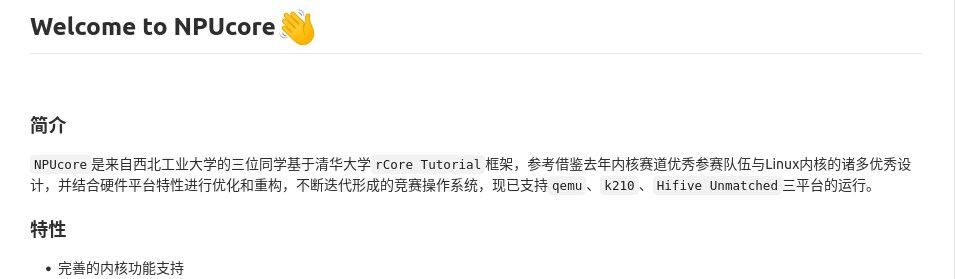
\includegraphics[width=\textwidth]{figures/02-01-readme.png}
	\caption{
		readme
	}
	\label{fig:readme}
\end{figure}
(2) help参数
绝大多数程序会自带一个help选项, 甚至不加任何参数。 例如, man命令的help参数:

\begin{lstlisting}[language={Rust}, label={code:forktest},
	caption={forktest.rs}]
	whatis --help
\end{lstlisting}

会打印出:
\begin{figure}[htb]
	\centering
	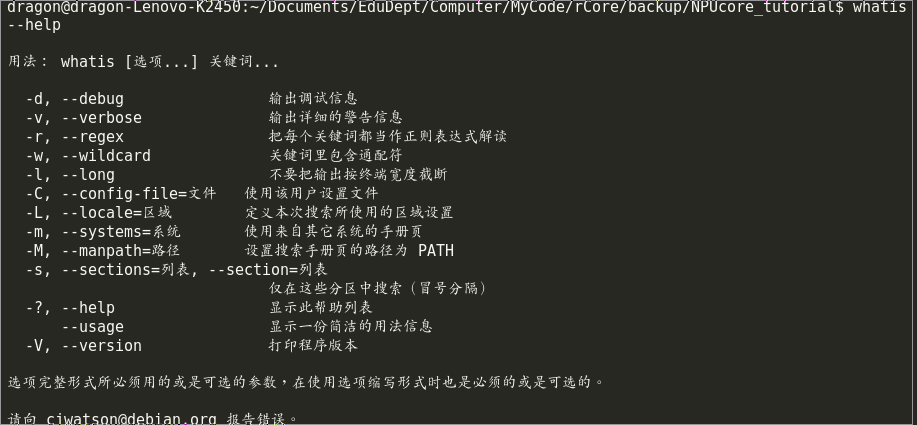
\includegraphics[width=\textwidth]{figures/02-01-help.png}
	\caption{
		help
	}
	\label{fig:help}
\end{figure}
那么, 如果你直接在终端中敲入help并回车, 会发生什么呢(假设你使用的是bash)?请自己试一下.

此外, 帮助文档的提供软件自身往往也会有自己的帮助文档, 显然自产自销是最合适的。

所以, 你不妨试一下man man, 或者进入man后有没有能看到的某些man自己的帮助文档(仔细找, 我这么说就一定有)。

之后的任何帮助套件也可以“自己帮助自己”, 所以文献中不再赘述。

(3) TAB补全

在Bash中,TAB补全是一种非常有用的功能,它可以让用户更快捷、更准确地输入命令和文件路径。在终端输入命令或文件路径时,如果按下TAB键,Bash会尝试自动补全输入的内容。

下面是关于Bash中TAB补全常见类型(如果没有特别说明, 则Bash会列出这些选项供选择):
1)命令补全:输入一个命令的前几个字母时,补全该命令的名称。如果有多个以该字符串开头的命令,
2)文件路径补全:输入一个文件或目录的路径时,补全路径中的文件或目录名称。如果有多个符合条件的文件或目录,
3)变量名补全:输入一个变量名时,补全该变量的名称。如果有多个符合条件的变量名,
4)命令参数补全:输入命令的参数时,补全该命令所支持的参数选项。如果有多个符合条件的参数选项,
5)目录补全:在输入路径时,如果您只知道路径中的某些部分,可以使用通配符进行补全。例如,输入"/u/lo*",按下TAB键可以自动补全为"/usr/local"。

总之,bash中的TAB补全是一种非常方便的功能,可以让用户更快速地输入命令和路径,并且减少输入错误的可能性。

此外, TAB补全需要程序自身和终端的支持, 有时候甚至需要单独配置, (例如rust的工具链就需要自行配置对应的shell补全选项)

\textbf{man}

在Linux操作系统中,man命令是一个非常重要的命令,它可以帮助用户查看Linux系统中各种命令的手册。

使用man只需要在终端中输入"man"加上要查看的命令名称,然后按下回车键即可。例如:

\begin{lstlisting}[language={Rust}, label={code:forktest},
	caption={forktest.rs}]
	man help
\end{lstlisting}

man命令将会显示出该命令的手册页,可以使用键盘上的箭头键进行滚动,并且可以使用“/”加上关键字进行查找。

在手册页中,可以查看该命令的使用方法、参数选项、示例以及其他相关信息。 man软件的本身的帮助信息可以在软件中按“h”查看。

当不再需要查看手册页时,可以按下“q”键退出man命令。

\textbf{完整手册}
多数成体系的大型软件系统会有自己对应的文档, 一般称为手册. 具体来说, 这种文档会出现在官方网站的Documentation环节, 且往往有在线或者线下PDF两种版本。

我们以GNU GCC为例, 在https://gcc.gnu.org/中, 浏览器搜索(一般快捷键是Ctrl-F)Documentation, 下方的Manual就是手册。点进去会有各种格式的手册。

有的成熟的软件或者语言会提供Tutorial 和 Reference Manual, 后者倾向于列举所有的性质, 前者则是为入门初学者提供的简单的教程。

一般而言, 绝大多数的软件是自身具有自己的手册的, 但部分软件的手册是集合型的, 或者本身就是其manpage的集合。

一个典型的例子是coreutils, 其中包括了cut, head, tail等简单工具;另一个是binutils, 包括各种GCC的常用工具。这时候需要自行查询其手册的所在之处。

\textbf{教材}

很多的软件都有自己的教材, 且层次从入门到精通都有, 如果你有需要, 可以找买一本合适的书从中学习。 一般教材会比官方手册更详细, 并提供作者自己的思考。

\textbf{TLDR}

TLDR是“Too long, don't read.”的缩写,
如果要最快获得某个命令的简单使用方法, tldr是一个不错的来源。例如我们输入

\begin{lstlisting}[language={Rust}, label={code:forktest},
	caption={forktest.rs}]
	$ tldr man
	
	Format and display manual pages.More information: https://www.man7.org/linux/man-pages/man1/man.1.html.
	
	- Display the man page for a command:
	man {{command}}
	
	- Display the man page for a command from section 7:
	man {{7}} {{command}}
	
	- List all available sections for a command:
	man -f {{command}}
	
	- Display the path searched for manpages:
	man --path
	
	- Display the location of a manpage rather than the manpage itself:
	man -w {{command}}
	
	- Display the man page using a specific locale:
	man {{command}} --locale={{locale}}
	
	- Search for manpages containing a search string:
	man -k "{{search_string}}"
\end{lstlisting}

\textbf{info}

注意, info是用某个目录作为中心数据库的, 所以完全可能存在在一个软件中可以阅读但在另一个软件中读不了的情况。

info中有大量长篇的完整文档, 一般就是上述完整手册。 一般各种IDE本身也会自带Info的阅读器。 只是info有自己的搜索, 历史记录等功能(有的功能是配合IDE使用的), 这里不再赘述。

此外, GNU套件几乎所有的工具都有info文档。所谓的GNU套件PDF文档就是用info相关的一个软件texinfo写的。

我们以gdb为例展示其内容。 终端输入“info gdb”可以得到:

\begin{figure}[htb]
	\centering
	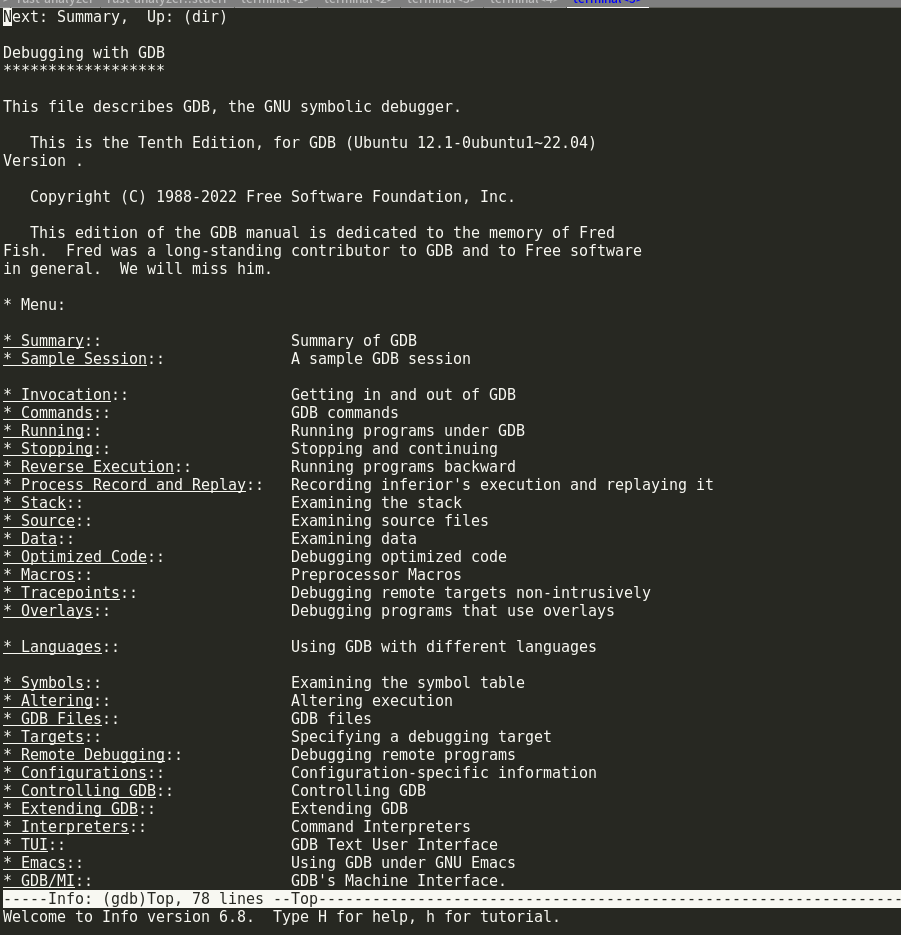
\includegraphics[width=\textwidth]{figures/02-01-info.png}
	\caption{
		info
	}
	\label{fig:info}
\end{figure}

另外, info文档的安装方法如下:

对于软件自带文档,一般可以:

\begin{lstlisting}[language={Rust}, label={code:forktest},
	caption={info}]
	sudo apt-get install gdb-doc
	有时候需要去网站上搜索并下载, 就会需要:
	whereis info # 获得info的安装目录
	# 注意:有时候下载到的是一个info.tar.gz, 这时候需要自行解压, 
	# 但是如果是info.gz,则可以直接跳过这一步, 因为gz一般是自动解压的。
	# 另外,有时候文档是以texi后缀名出现的
	tar xf <infofilepath> <tmp_path>
	sudo install-info bison.info <one_of_the_info_paths>/dir
\end{lstlisting}

\textbf{自动补全与文档显示插件}

多数的IDE有自己的文档现实和自动补全插件, 可以在光标悬停在某个符号一段时间后自动显示特定的文档。

很多IDE还会集成之前的所说的这些文档查询方式, 从而在内部查询所有的文献。

请自行搜索自己的编辑器和IDE的文档寻找配置方式。

\textbf{搜索引擎}

如果你遇到什么工具你无法使用或者不会用, 可以尝试通过搜索引擎寻找替代品, 在线版或者其他能让你用上的方法(比如能够代理你请求的某些接口,软件和网站)。

\textbf{论坛}

论坛往往是最后一步, 一般来说很少出现别人没有发现过而自己发现的问题, 毕竟计算机工业确实过于发达了. 但是, 在stackoverflow和其他论坛上提问仍然有可能可以获得比较好的效果。

如果人家恰好碰到过或者有兴趣帮你解决问题的话是再幸运不过的事, 不过在此之前, 请先不要往下看, 尝试通过之前几步查找可能技术论坛以便解决问题。

然后这是一份作者根据自己回忆写的常见的论坛, 你可以试着在上面发帖. 此外, 一般使用量大的项目都有自己的论坛, 你也可以自行查找。









\chapter{相关工作(Related Work)}

为了取长补短,我们这里将与NPUcore-IMPACT优化相关的工作总结到本章节中。
\section{NPUcore系统调用性能分析}
我们对比了往年的OSKernel大赛优胜,与我们NPUcore-family的多种性能,以便从中获取到关键优化信息。
首先我们给出NPUcore,基准程序,与两个其它内核Titanix和PLNTRY在libc-bench和Unixbench测例上的耗时与得分(如表\ref{table:score1}和\ref{table:score2})。

\begin{table}
    \centering
    \label{table:score1}
    \resizebox{\linewidth}{!}{
    \begin{tabular}{|l|c|c|c|c|}
        \hline
        \textbf{测例}                                   & \textbf{NPUcore}  & \textbf{基准程序}      & \textbf{Titanix}     & \textbf{PLNTRY}\\
        \hline
        b\_malloc\_sparse (0)                           &   -                   & 0.325008007           & 0.307474000       & 0.749882000           \\
        \hline                      
        b\_malloc\_bubble (0)                           &   -                   & 0.299156383           & 0.302118000       & 0.795564000           \\
        \hline                      
        b\_malloc\_tiny1 (0)                            &   -                   & 0.011439820           & 0.010716000       & 0.020421000           \\
        \hline    
        b\_malloc\_tiny2 (0)                            & 0.005085920           & 0.008827947           & 0.008677000       & 0.013895000           \\
        \hline      
        b\_malloc\_big1 (0)                             &   -                   & 0.089668000           & 0.089668000       & 0.205780000           \\
        \hline
        b\_malloc\_big2 (0)                             & 0.028311200           & 0.092570898           & 0.089264000       & 0.159222000           \\
        \hline
        b\_malloc\_thread\_stress (0)                   & 0.066339520           & 0.078210295           & 0.088639000       & 0.065488000           \\
        \hline
        b\_malloc\_thread\_local (0)                    &   -                   & 0.076371644           & 0.084808000       & 0.057541000           \\
        \hline
        b\_string\_strstr ("abcdefghijklmnopqrstuvwxyz") & 0.011712000          & 0.014879018           & 0.014637000       & 0.014606000           \\
        \hline
        b\_string\_strstr ("azbycxdwevfugthsirjqkplomn") & 0.017838240          & 0.022160122           & 0.022694000       & 0.022971000           \\
        \hline
        b\_string\_strstr ("aaaaaaaaaaaaaacccccccccccc") & 0.011262640          & 0.013371076           & 0.014105000       & 0.014078000           \\
        \hline
        b\_string\_strstr ("aaaaaaaaaaaaaaaaaaaaaaaaac") & 0.010942000          & 0.013494579           & 0.014031000       & 0.013603000           \\
        \hline
        b\_string\_strstr ("aaaaaaaaaaaaaaaaaaaaaaaaaaaaaaaac") & 0.013523120   & 0.016474362           & 0.017411000       & 0.017628000           \\
        \hline
        b\_string\_memset (0)                            & 0.009740400          & 0.010840004           & 0.012793000       & 0.012005000           \\
        \hline
        b\_string\_strchr (0)                            & 0.011392640          & 0.013300974           & 0.015052000       & 0.014630000           \\
        \hline
        b\_string\_strlen (0)                            & 0.009787360          & 0.011389320           & 0.013102000       & 0.012690000           \\
        \hline
        b\_pthread\_createjoin\_serial1 (0)              & 0.439336960          & 1.087431144           & 1.643873000       & 1.048143000           \\
        \hline
        b\_pthread\_createjoin\_serial2 (0)              & 0.426977760          & 0.861784643           & 1.791139000       & 1.020008000           \\
        \hline
        b\_pthread\_create\_serial1 (0)                  & 0.476990480          & 0.785009610           & 2.702702000       & 2.689056000           \\
        \hline
        b\_pthread\_uselesslock (0)                      & 0.060514480          & 0.067189695           & 0.079902000       & 0.078151000           \\
        \hline
        b\_utf8\_bigbuf (0)                              & 0.032511520          & 0.035250394           & 0.035864000       & 0.037977000           \\
        \hline
        b\_utf8\_onebyone (0)                            & 0.091743280          & 0.114485028           & 0.116207000       & 0.117029000           \\
        \hline
        b\_stdio\_putcgetc (0)                           & 0.439399360          & 0.764247677           & 0.621226000       & 0.361184000           \\
        \hline
        b\_stdio\_putcgetc\_unlocked (0)                 & 0.426097680          & 0.752266360           & 0.615693000       & 0.339361000           \\
        \hline
        b\_regex\_compile ("(a|b|c)*d*b")                & 0.057043200          & 0.071444121           & 0.073049000       & 0.075878000           \\
        \hline
        b\_regex\_search ("(a|b|c)*d*b")                 &   -                  & 0.081086193           & 0.083481000       & 0.086110000           \\
        \hline
        b\_regex\_search ("a\{25\}b")                    &   -                  & 0.254820207           & 0.253847000       & 0.256301000           \\
        \hline
    \end{tabular}
    }
    \caption{libc-bench耗时,“-”代表NPUcore无法正常执行。}
\end{table}

\begin{table}
    \centering
    \label{table:score2}
    \resizebox{\linewidth}{!}{
    \begin{tabular}{|l|c|c|c|c|}
        \hline
        \textbf{测例}                       & \textbf{NPUcore}      &\textbf{基准程序}  & \textbf{Titanix}   & \textbf{PLNTRY}\\
        \hline
        Unixbench DHRY2 test(lps)           & 61405230              &49005063       & 49932495              & 48523418  \\
        \hline
        Unixbench WHETSTONE test(MFLOPS)    & 1269.670              &1026.820       & 997.612               & 1014.102  \\
        \hline
        Unixbench SYSCALL test(lps)         & 222615                &2416696        & 1216209               & 547678    \\
        \hline
        Unixbench CONTEXT test(lps)         & 168113                &80174          & 54440                 & 42416     \\
        \hline
        Unixbench PIPE test(lps)            & 413979                &330556         & 162389                & 802449    \\
        \hline
        Unixbench SPAWN test(lps)           & 64394                 &16686          & 14937                 & 13586     \\
        \hline
        Unixbench EXECL test(lps)           & 73597                 &6645           & 1262                  & -         \\
        \hline
        Unixbench ARITHOH test(lps)         & 7032261867            &5718673825     & 5607494736            & 5541357804\\
        \hline
        Unixbench SHORT test(lps)           & 179342297             &147678033      & 141948434             & 140413305 \\
        \hline
        Unixbench INT test(lps)             & 179660281             &148128134      & 140942140             & 140311940 \\
        \hline
        Unixbench LONG test(lps)            & 179644882             &153417287      & 141540178             & 140287530 \\
        \hline
        Unixbench FLOAT test(lps)           & 178725171             &148049012      & 141550560             & 142030413 \\
        \hline
        Unixbench DOUBLE test(lps)          & 179034748             &148031827      & 142851862             & 141484435 \\
        \hline
        Unixbench HANOI test(lps)           & 677685                &544504         & 545068                & 536762    \\
        \hline
        Unixbench EXEC test(lps)            & 39493                 &945            & 8561                  & -         \\
        \hline
    \end{tabular}
    }
    \caption{Unixbench测试分数,“-”代表PLNTRY无法正常执行。}
    \label{Unixbench测试结果}
\end{table}
我们可以看到,NPUcore的耗时均比基准程序短,Unixbench得分均比基准程序高,这说明NPUcore相较于基准程序,我们在时间维度上性能提升许多,但是我们仍有一些测例无法通过。
例如对于缓存相关测试,NPUcore使用较为激进的缓存策略,Page Cache容量不设上限,所有的内存空间都可以作为缓存使用。即使发生内存不足,NPUcore会根据LRU算法清理无用缓存。
经过测试发现,在这种缓存策略下运行大多数测例时,对每个文件NPUcore只从外存读取一次,之后的读写全部发生在Cache中,从而带来极大的性能提升。
而因为对于比赛而言,和基准程序比较不能说明太多问题,应与其它参赛队伍比较,这点我们会在下面详细分析。

\section{其他内核系统调用性能分析}


\subsection{Titanix}

首先,从\href{https://gitlab.eduxiji.net/202318123101314/oskernel2023-Titanix}{https://gitlab.eduxiji.net/202318123101314/oskernel2023-Titanix}地址克隆仓库,切换到master分支。根据其README说明,
进入kernel目录并运行sudo make fs-img,镜像构建完成后运行make run启动内核,在内核中运行runtestcase开始运行测例。



通过比较 NPUcore 和 Titanix 的 libc-bench 和 Unix-bench 可以发现,在 libc-bench 中,
NPUcore 的和 Titanix 的所耗时间比较相似,不过NPUcore对于进程的创建要表现得更好一些。在 Unix-bench 中,Titanix的部分性能优于NPUcore,例如
SYSCALL (lps),而NPUcore在其他方面的得分均略高于Titanix,特别是EXEC test(lps)。

对于Titanix性能表现的分析:
\begin{itemize}
    \item 内存管理:
    实现了页缓存和块缓存以减少IO次数,实现懒分配和写时复制以优化性能。
    Titanix的懒分配包括三个方面:(1)用户栈的懒分配,进程构建出来时只分配虚拟地址栈空间,当用户访问栈空间时再通过缺页中断分配物理页
    (2)用户堆的懒分配,与用户栈的懒分配相似,当用户真正读写该堆空间时再通过缺页中断进行物理页分配。(3)mmap 内存段的懒读取,当用户进行 mmap 系统调用时,记录下对应的文件指
    针以及映射的偏移量范围但不进行实际读取,当用户真正读写到该内存段时再通过缺页中断读取相应文件的相应位置的内容。
    Titanix的写时复制主要指在进行 fork 系统调用构造出新的进程时,不需要将父进程地址空间的全部内
    存拷贝一份,而是让子进程与父进程共享物理内存页,这样做的开销就只有修改页表。同时如果某个内存段是懒分配的内存
    段,便不需要共享物理页,直接新增一个虚拟地址内存段即可。
    \item 进程管理:
    Titanix 采用无栈协程的调度方式,所有线程(包括不同进程的线程)共享同一个内核栈,调度起来开销比较小。因为所有协程共用一个栈,所以需要每个协程在堆上维护一个状态机,通过轮询
    当前的状态进行协程的切换,然后根据状态决定是否需要切换。无栈协程的调度是通过函数返回然后调用另一个函数实现的,而不是像有栈协程那样直接原地更改栈指针。也带来了一定程度的性能优化和安全性保证。
    \item 文件系统:
    实现了Inode缓存,可以减少IO次数:Titanix通过设置全局对象 INODE_CACHE,来对可能会使用的 inode 进行缓存,Inode缓存主要用于完成某一个文件的 inode 的文件名哈希值与 inode 自身的映射管理。这样一来,在
    频繁的访问Inode时可以减少一部分因为查找带来的IO访问磁盘时延,从而达到优化性能的效果。
    
    Titanix通过在Inode和实际文件名之间建立哈希映射来实现对文件的快速查找:当传入一个文件名时,调用实现的 hash_name 方法进行哈希值的计算,并从构建的全局哈希表当中获取该 inode 的
    Arc 引用,即查找到了对应文件。


\end{itemize}

\subsection{PLNTRY}

首先,从\href{https://gitlab.eduxiji.net/PLNTRY/OSKernel2023-umi/-/blob/comp3-coverage}{https://gitlab.eduxiji.net/PLNTRY/OSKernel2023-umi/-/blob/comp3-coverage}地址处克隆仓库,
切换到master分支。将比赛提供的镜像文件复制到OSKernel2023-umi/third-party/img文件目录下,
命名为sdcard-comp2.img,在主文件目录下make all,make run即可运行该kernel。
所有的测试结果不直接在终端显示,而在qemu.log中显示。




通过比较NPUcore和PLNTRY的libc-bench和Unix-bench可以发现,在libc-bench中,NPUcore的和plntry的所耗时间比较相似,这与测例的相对简单有比较大的关系。但是在Unix-bench中,plntry的部分性能得分优于NPUcore。例如SYSCALL (lps),CONTEXT (lps),PIPE (lps),当然NPUcore也有比plntry表现更良好的测试项,比如DHRY2 test(lps), SPAWN test(lps)等。

“syscall”测试是一个基准测试,用于评估系统在执行系统调用(syscalls)时的性能。系统调用是操作系统提供给用户空间程序访问操作系统内核功能的接口。
这个测试旨在测量系统在执行各种系统调用时的效率和速度。UnixBench会执行一系列常见的系统调用,比如文件操作、进程控制、内存管理等,然后测量系统在执行这些调用时所需的时间和性能。
“syscall”测试的结果以每秒钟能够执行的系统调用数量(lps-syscalls per second)作为单位,因此其结果值越高表示系统在处理系统调用时的效率越高,执行系统调用的能力也就越强。

UnixBench中的“CONTEXT”测试是用来评估系统在上下文切换方面的性能。上下文切换是操作系统在多任务环境中切换执行不同进程或线程时所需的过程。
“CONTEXT”测试测量系统在进行上下文切换时的效率,它涉及将处理器从一个进程或线程切换到另一个的能力。在多任务系统中,上下文切换是一种常见操作,而系统的性能可能会受到其影响。
测试结果以每秒钟能够完成的上下文切换数量(lps-context switches per second)作为单位。因此,较高的数值表示系统在处理上下文切换时更有效率,能够更快地在不同的进程或线程之间进行切换。

"spawn" 测试是一个基准测试,用于评估系统在并发进程创建和销毁方面的性能。该测试模拟了系统同时启动多个进程的情况,然后检查系统在这种高并发情况下的性能表现。
"spawn" 测试通常会创建许多子进程,然后立即销毁它们,以测试系统处理这些操作的速度和效率。这个测试可以显示系统在处理并发任务时的能力,因为进程的创建和销毁在某些应用场景下可能是非常常见的操作。
UnixBench中的 "spawn" 测试的结果以每秒钟能够创建和销毁的进程数(lps-processes per second)作为单位,因此其结果值越高表示系统在这个方面的性能越好。


性能优秀的原因:
\begin{itemize}
    \item 内存管理:在页帧管理实现写时复制策略和通用 IO 缓
存,减少 IO 设备访问次数。
在地址空间管理实现懒分配策略,提高内存.

在设计UMI的页帧管理模块的部分,借鉴 Fuchsia 设计了一套 RAII 的基于二叉树形的数据结构。
每个节点逻辑上是其父节点的一个切片,有标志指示是否拥有写时复制(CoW)特性。
页帧通过引用计数和缓存状态的更新在树形结构中复制和流动。例如在提交页帧的时候,
依次从自身的哈希表、父节点的哈希表、I/O 后端读写、新清零页的顺序来依次访问并提
交页帧。

通过如上说明可以看到,Phys 结构体可以作为任意读写+寻址的后端的页缓存,包
括普通文件、块设备等。这样,虽然缺乏了一些特定场景的优化,可以避免重复的页缓
存代码。并且由于写时复制和懒分配两个特性,任何涉及到内存分配的场景都会获得对应的
性能提升。同时,每个节点可以实现同时读写页帧,在不浪费页帧的情况下提升页缓存的并
发性。
    \item 线程管理与调度:使用细粒度锁和 Rust 所有权系统管理线程
的本地状态和信息
支持软抢占和任务窃取的 SMP 多核调度器
基于有栈协程模式的特权级切换

传统的操作系统往往采用有栈协程将任务的调用栈和上下文分开保存,通过汇编代码手动
切换函数调用栈来进行任务切换。每个任务的调用栈都会有一定的内存浪费(空闲),并都
会有栈溢出风险。

而无栈协程则将任务的信息同一保存成状态机,统一存放在堆上,由执行器通过更改指
针来切换执行的任务。从图中我们可以发现,调用栈仅与每个执行器一一绑定,一定程度上
减少了内存浪费、降低栈溢出风险。

    \item 文件系统:统一的虚拟文件系统接口
支持 debugfs、FAT32、procfs、devfs 等多
种存储和内存文件系统。本身并没有很多创新之处。
    \item 网络协议栈:基于 smoltcp 的多设备接口网络协议栈
TCP 独立的 ACCEPT 队列
\end{itemize}



\section{基于GDB内核调试}
在软件开发过程中,调试是不可避免的。一个程序往往不会一开始就按照程序员预期的方式运行, 对操作系统这样的复杂巨系统而言尤其如此。本节主要讲解调试软件GDB的使用方法。
\subsection{认识GDB}
GNU调试器(英语:GNU Debugger,缩写:GDB),是GNU软件系统中的标准调试器,此外GDB也是个具有移携性的调试器,经过移携需求的调修与重新编译,如今许多的类UNIX操作系统上都可以使用GDB,而现有GDB所能支持调试的编程语言有C、C++、Pascal以及FORTRAN。

\textbf{为什么需要GDB}

当程序出现错误时,开发者需要快速地找出错误的原因,并修复它们。很多人会倾向于使用"人工静态分析"(也就是目测法和冥想法)解决Bug。

然而,程序的运行时状态往往非常复杂,有时很难在代码中准确地定位错误。 具体来说, 目测的以下缺点导致开发者往往会百思不得其解进而无功而返:

\textbf{1.无法检测运行时问题:}代码静态分析只能检测静态代码问题,例如语法错误、类型错误等,它无法检测代码的运行时问题。例如,它无法检测到由于代码在特定环境下执行而引起的问题,如内存泄漏、死锁等。

\textbf{2.误报和漏报:}静态分析可能会误会遗漏问题。例如,可能会将某些无害的代码标记为错误,或者忽略某些实际上是错误的代码。这可能会导致开发人员浪费时间和精力来调查错误的根本原因。

\textbf{3.对高质量代码的依赖:}代码静态分析需要高质量的代码才能进行准确的分析。如果代码质量不好,例如缺乏注释、变量名不规范、代码冗余等,那么静态分析可能会产生误报或漏报。

\textbf{4.难以发现复杂的问题:}静态分析工具通常使用各种分析技术来分析代码,但这些技术很难发现复杂的问题,例如多线程问题、分布式系统问题等。这些问题通常需要动态调试或其他更高级的技术来解决。

同样, 也有人会尝试插入LOG打印部分状态, 但是这种方法除了费时费力, 且暴露状态不够精确的问题之外, 在OS中, 某些LOG会产生系统状态的改变, 进而影响结果, 导致debug失败。

这时候,调试工具就显得非常重要了。调试工具可以帮助开发者在运行时监视程序的状态,跟踪代码的执行流程,查看变量的值,以及定位错误的位置。 这正是GDB的用途。

GDB 最初由Richard Stallman在他的GNU Emacs 系统稳定后于1986年编写,并设计作为他的GNU系统的一部分。GDB是根据GNU通用公共许可证(GPL)发布的免费软件。它是在Berkeley Unix发行版附带的DBX调试器之后建模的。从1990 年到 1993 年,它由John Gilmore维护。现在由自由软件基金会任命的 GDB 指导委员会维护。

GDB允许用户查看一个程序在执行时“内部”的执行过程—,或者查看程序在崩溃时的内部状态。这些被调试的程序可以与 GDB 在同一台机器上(本地)、另一台机器(远程)或模拟器上执行。GDB 可以在大多数流行的 UNIX 和 Microsoft Windows 变体以及 Mac OS X 上运行。具体而言,目前 GDB 支持以下程序:Ada、Assembly、C、C++、D、Fortran、Go、Objective-C、OpenCL、Modula-2、Pascal、Rust 等。

GDB 默认只有命令行接口(CLI)可用,而不具备较能亲合上手、直觉操作的图形用户界面(GUI),不过此一弱处也已经有几个前端程序为其补强,例如DDD、GDBtk/Insight (页面存档备份,存于互联网档案馆)以及Emacs中的“GUD 模式”等,有了这些补强后,GDB在功效使用的便利性上就能够与“集成发展环境中的调试功效使用”相接近。

\textbf{GDB的启动}

显然, 启动gdb有不同的方法, 在终端中输入gdb是最简单的, 但NPUcore在RISC-V上构建, 因此不能直接使用本机的gdb(除非你使用一台RISC-V64计算机),因此我们推荐安装并使用gdb-multiarch(这里需要Ubuntu环境):
\begin{lstlisting}[language={Rust}, label={code:forktest},
	caption={forktest.rs}]
	$ sudo apt-get install gdb-multiarch
	# 然后启动:
	$ gdb-multiarch
\end{lstlisting}

注意, 这里实际上有"工作目录"的概念, 也就是你的当前目录实际上最好在项目或者源代码的路径上, 否则会需要手工加载源代码路径(方法见下文)。
\subsection{基于GDB的内核调试}
\textbf{QEMU虚拟机的相关命令}

介绍GDB为什么要先介绍虚拟机呢?因为正是QEMU与GDB合作, 才给了我们方便地进行大部分系统软件调试的机会。

作为一款全虚拟化虚拟机, QEMU能彻底模拟CPU的内部状态, 包括寄存器和其他部分, 因此很适合进行调试。

具体来说, QEMU配合GDB提供了单步执行、断点调试、内存监视、寄存器查看等。

用户可以使用调试功能逐步执行代码,查看每一步的运行结果和寄存器状态,同时还可以设置断点,方便定位问题所在。

利用QEMU提供的远程调试功能,允许用户在另一台计算机上通过网络连接到QEMU的调试接口进行调试。这个功能可以方便地在不同的计算机之间进行协作开发和调试。

这里我们只介绍本地的远程调试。

为了方便, 在os文件夹中, 使用下列make命令直接进行gdb调试:
\begin{lstlisting}[language={Rust}, label={code:forktest},
	caption={forktest.rs}]
	make gdb
\end{lstlisting}
其后端执行实际命令是:
\begin{lstlisting}[language={Rust}, label={code:forktest},
	caption={forktest.rs}]
	gdb:
	@qemu-system-riscv64 -machine virt -nographic -bios $(BOOTLOADER) -device loader,\
	file=target/riscv64gc-unknown-none-elf/debug/os,addr=0x80200000 -drive \
	file=$(U_FAT32),if=none,format=raw,id=x0 \
	-device virtio-blk-device,drive=x0,bus=virtio-mmio-bus.0 -smp threads=$(CORE_NUM) -S -s
\end{lstlisting}  
和do-run的内容相比,
\begin{lstlisting}[language={Rust}, label={code:forktest},
	caption={forktest.rs}]
	do-run:
	@qemu-system-riscv64 \
	-machine virt \
	-nographic \
	-bios $(BOOTLOADER) \
	-device loader,file=$(KERNEL_BIN),addr=$(KERNEL_ENTRY_PA) \
	-drive file=$(U_FAT32),if=none,format=raw,id=x0 \
	-device virtio-blk-device,drive=x0,bus=virtio-mmio-bus.0\
	-smp threads=$(CORE_NUM)
\end{lstlisting}  
不难发现最主要的差别在于后面多出的"-S -s"。 前面的S代表STOP, 意思是设置完虚拟机直接挂起, 停止一切执行, 直到接收到外部的continue信息为止.

第二个小写s等价于"-gdb tcp::1234",指的是开启远程调试,其在localhost(本机)的1234端口侦听GDB的信号, 等待连接。 然后, 就是我们的下一个工具GDB的任务和工作范畴了。

\begin{figure}[htb]
\centering
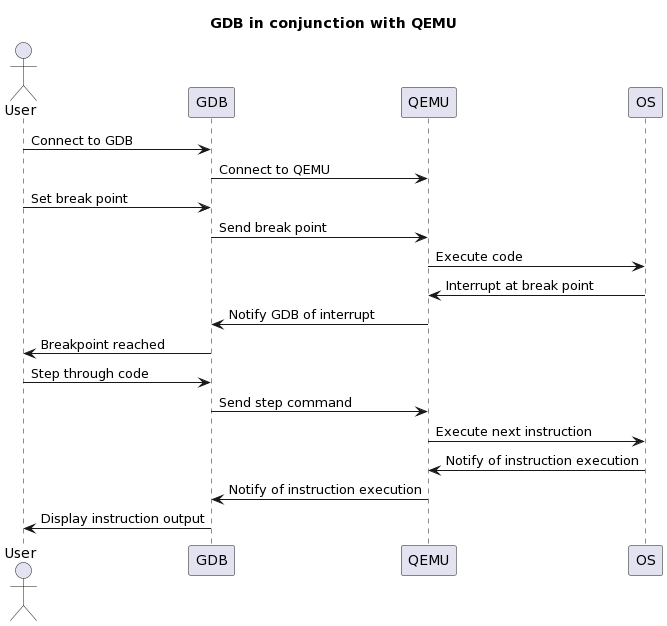
\includegraphics[width=\textwidth]{figures/02-02-GDB联调QEMU的逻辑流程.png}
\caption{
	GDB联调QEMU的逻辑流程
}
\label{fig:GDB联调QEMU的逻辑流程}
\end{figure}

\textbf{历史}
在GDB的命令行(和各种IDE的GDB控制台)中, 使用上下左右(或者Alt-P之类的自定义按键)可以直接显示之前的命令, 这和Bash是一致的。

但和Bash不同的是, 其重复执行上一条命令可以通过直接在不进行任何输入的时候敲回车实现:

\begin{lstlisting}[language={Rust}, label={code:forktest},
	caption={forktest.rs}]
	(gdb) stepi
	(gdb) (然后这里敲回车)
\end{lstlisting} 

这时候就前进了两条指令。但这个功能也会导致有时候多按了一下回车结果重复执行了某些只应当被执行一次的指令, 因此也要注意使用的场景。
\textbf{补全}

GDB命令的确数量庞大且内容复杂, 但是但作为一款老牌软件, GDB自然也有解决方案。一方面, GDB自己提供了强大的命令补全功能, 能像在Bash中一样TAB补全,例如如下所示的键盘输入:输入b然后按下TAB键, 会补全为break, 其他的, 如寄存器名称等往往也可以在有了部分提示前缀后进行补全。 因此不需要每次都键入完整的命令。

\textbf{辅助}

另一方面, 多数的IDE和编辑器都有辅助GDB的功能, 例如在某一行代码旁边点击行号附近的位置, 会出现一个圆点, 表示加入断点。

另外, 如果你需要重复某个命令多遍, 并不需要一直按着鼠标或者键盘回车键, 只需要在命令后面插入重复次数即可:

\begin{lstlisting}[language={Rust}, label={code:forktest},
	caption={forktest.rs}]
	(gdb) stepi 4
\end{lstlisting}

这里就前进了4条指令。

\textbf{常见命令}

进入gdb, 会看到"(gdb)"提示可以输入命令(有时候无法输入)。

如果在VSCode中使用, 还需要在之前加上exec

\begin{lstlisting}[language={Rust}, label={code:forktest},
	caption={forktest.rs}]
	exec gdb <...>
\end{lstlisting}

\textbf{设定命令}
(1) 连接

按照之前的方法启动QEMU后, GDB要通过下列命令连接本地的QEMU。

\begin{lstlisting}[language={Rust}, label={code:forktest},
	caption={forktest.rs}]
	target remote :1234
	
	<div align=center><img src="./pic/1.2/remote.png" style="zoom:100%"></div> 
	
	如果你之前指定了自定义的端口, 需要将1234换成其他的端口号。同时, 冒号之前实际上省略了localhost(也就是本机的“网址”), 如果你将来有自定义的地址或者网址, 也可以在前面补上。
\end{lstlisting}

(2) 加载调试信息

\begin{lstlisting}[language={Rust}, label={code:forktest},
	caption={forktest.rs}]
	(1)file
	在开始调试之前, 你首先需要加载调试信息。
	file target/riscv64gc-unknown-none-elf/debug/os
	从而加载os文件作为符号文件。请注意, 使用release版本的文件(在make命令中加入“MODE=release”得到)往往不带有任何的调试信息, 不适合用于debug, 但也不尽然: 你可以对着汇编语言调试。 当然, 就算使用了带有符号文件的版本,这种体验你总会遇到的, 因为操作系统总是要涉及某些底层。
	这里加载的是操作系统的符号, 那如果某些过程经过用户程序(作为一个操作系统, 你总会遇到这种问题), 如何添加用户程序的代码?这就要用到一下一个命令了。
	如果先连接QEMU后加载二进制文件, 就会出现上面的"A program is being debugged already."提示,当然这并不影响使用。
	
	$add-symbol-file
	
	$ add-symbol-file bash
	
\end{lstlisting}

如果你的当前工作文件夹中具有bash文件, 就可以直接添加, 否则需要自行前往特定的。 显然, 上面两个命令的顺序可以修改, 但注意, file只能有一个, symbol-file却可以有很多, 且符号文件指代的不一定是带有符号部分的可执行文件, 也可能是纯粹的符号文件(考虑到其和主题无关,这里的内容我们不拓展,读者可以进一步查找资料)。 这时候可以info files显示所有已经添加的符号和二进制文件

\begin{figure}[htb]
\centering
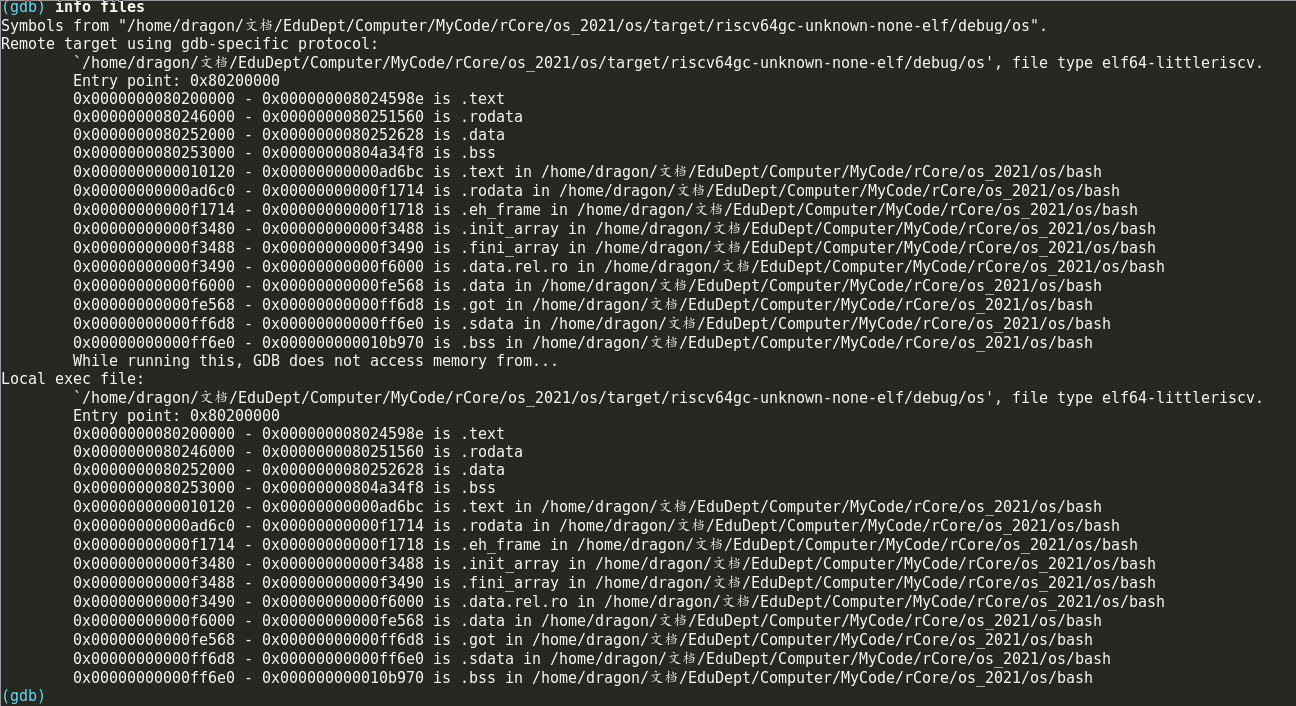
\includegraphics[width=\textwidth]{figures/02-02-info files.png}
\caption{
	info files
}
\label{fig:info files}
\end{figure}

\begin{lstlisting}[language={Rust}, label={code:forktest},
	caption={forktest.rs}]
	(1)directory
	设置完符号文件, 接着需要设置源代码目录, 这样在IDE/GDB中可以自动跳转到函数代码所在处。
	$dir ~/Downloads/SW/Bash/bash-5.1.16/
	$dir ~/Downloads/SW/Bash/bash-5.1.16/lib/sh/
	注意, 这里需要你将bash的源代码先提前下载好到某个目录, 并将上面的这个路径替换成正确的目录。
	最终得到:
	Source directories searched: /home/dragon/Downloads/SW/Bash/bash-5.1.16/lib/sh:/home/dragon/Downloads/SW/Bash/bash-5.1.16:$cdir:$cwd
	另外,部分的软件目录结构复杂, 这时候需要手动用上述命令添加。
	(2)break
	break用于设置断点。可以通过断点中断程序的执行并让你进入调试模式。
	一般常见的断点设定方式有:文件:行号格式和函数(方法)格式
	例如:(基于特定版本, 你的具体地址与行号可能不同)
	$(gdb) b src/main.rs:50
	Breakpoint 1 at 0x900000000004f158: file src/main.rs, line 59.
	$(gdb) b rust_main
	Breakpoint 2 at 0x900000000004f198: file src/main.rs, line 66.
	
	注意! 函数名方法有时候要指定域, 格式类似os::rust_main;
	如果要删除断点, 则可以
	$delete 1
	跟上断点号即可。
	(3)set
	set可以是多种的, 最典型的是让pc强制移动到某个位置, 例如:
	$set $pc=0x0
	回到最开始的执行点。 当然, 你也可以用它对别的地址/变量进行强行赋值。
	
\end{lstlisting}

\textbf{执行流}

(1)continue
很显然, GDB有两种状态, 停止和执行, 只有在停止的时候, 我们才能对其中的数据进行查看和修改, 对自己的命令进行调整,而continue正是从停止到执行的切换工具。

continue会继续执行程序直到遇到下一个断点或程序结束。 这条命令往往用于target remote :1234后继续执行。

例如, 我们一开始执行make gdb只有:

\begin{lstlisting}[language={Rust}, label={code:forktest},
	caption={forktest1.rs}]
	$ make gdb
\end{lstlisting}

一个光标停在原地。

但是, 如果你在gdb中输入continue并回车, 虚拟机马上就会停止冻结,开始执行指令(直到撞到某个停止条件为止):

\begin{figure}[htb]
\centering
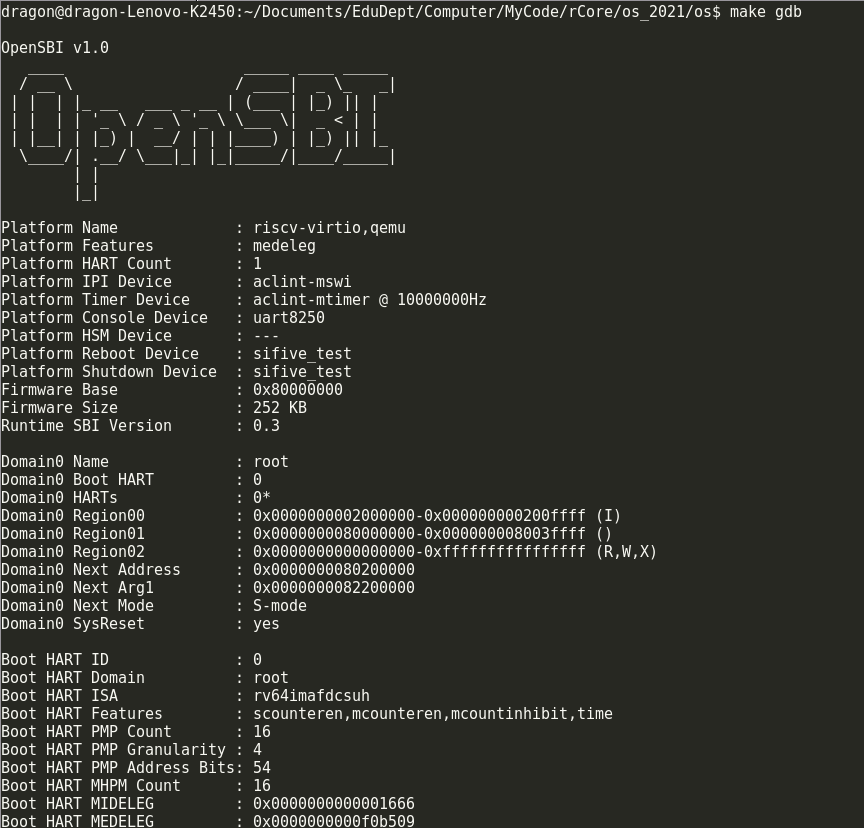
\includegraphics[width=\textwidth]{figures/02-02-设置断点.png}
\caption{
	设置断点
}
\label{fig:设置断点}
\end{figure}

此时, 命令就会停在之前设定的断点上
(2)暂停或终止运行

在终端和多数IDE中, 暂停执行流是通过gdb控制台(注意不是虚拟机的终端, 而是gdb的控制台)ctrl-C(同时按下Ctrl和C)实现的, 这可以让程序暂停在当前执行到的位置。

如果你之前在执行QEMU时没有加入“-S”选项, 那么你可以用这条命令立即暂停执行流(当然其具体停止位置难以保证。)

完成后debug后, 可以用quit退出。

(3)next,step和finish

stepi前进一条指令.

\begin{figure}[htb]
\centering
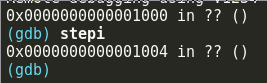
\includegraphics[width=\textwidth]{figures/02-02-stepi.png}
\caption{
	stepi
}
\label{fig:stepi}
\end{figure}

next可以单步执行程序,跳过函数调用,例如(中间省略几步continue和break):

\begin{figure}[htb]
\centering
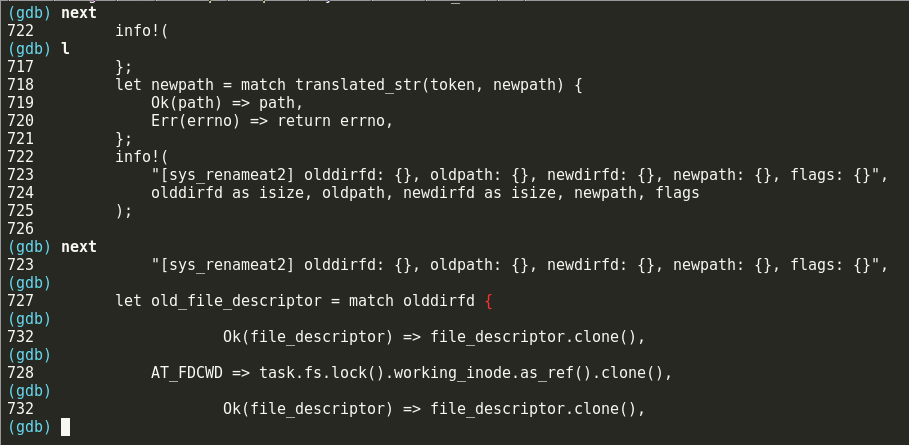
\includegraphics[width=\textwidth]{figures/02-02-next.png}
\caption{
	next
}
\label{fig:next}
\end{figure}

可以看到这里的几条函数都被跳过了。

step单步执行程序,进入函数调用(这里的执行流进入了函数调用):

\begin{figure}[htb]
\centering
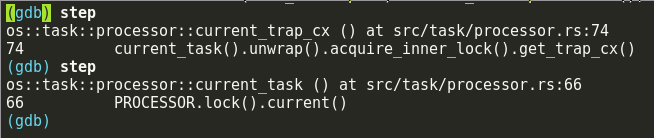
\includegraphics[width=\textwidth]{figures/02-02-step.png}
\caption{
	step
}
\label{fig:step}
\end{figure}

finish执行完当前函数并返回到调用函数, 然后又回到了之前的函数:

\begin{figure}[htb]
\centering
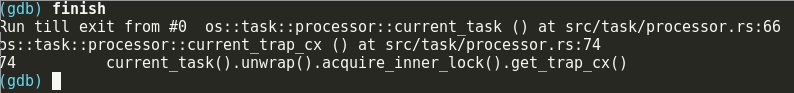
\includegraphics[width=\textwidth]{figures/02-02-finish.png}
\caption{
	finish
}
\label{fig:finish}
\end{figure}

\textbf{查看命令}

在停止状态下, 我们可以backtrace显示函数调用栈:

\begin{figure}[htb]
\centering
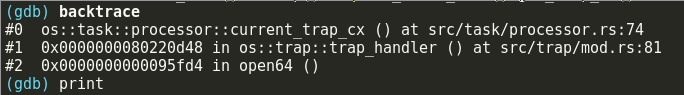
\includegraphics[width=\textwidth]{figures/02-02-backtrace.png}
\caption{
	backtrace
}
\label{fig:backtrace}
\end{figure}

或者print打印寄存器/变量/内存地址的值:

\begin{figure}[htb]
	\centering
	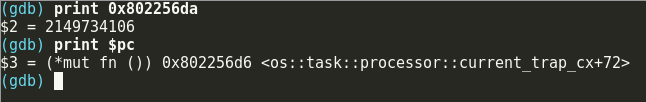
\includegraphics[width=\textwidth]{figures/02-02-print.png}
	\caption{
		print
	}
	\label{fig:print}
\end{figure}

如果觉得每次都打印很麻烦,可以用display每次停在断点处时自动打印某个变量的值。一旦不需要, 可以undisplay该号码取消(类似delete语法),如下列这段话打印附近前后各6条汇编代码(其他的变量也可以打印,语法类似)

\begin{lstlisting}[language={Rust}, label={code:forktest},
	caption={forktest1.rs}]
	display/12i $pc-6*4
\end{lstlisting}

\begin{figure}[htb]
\centering
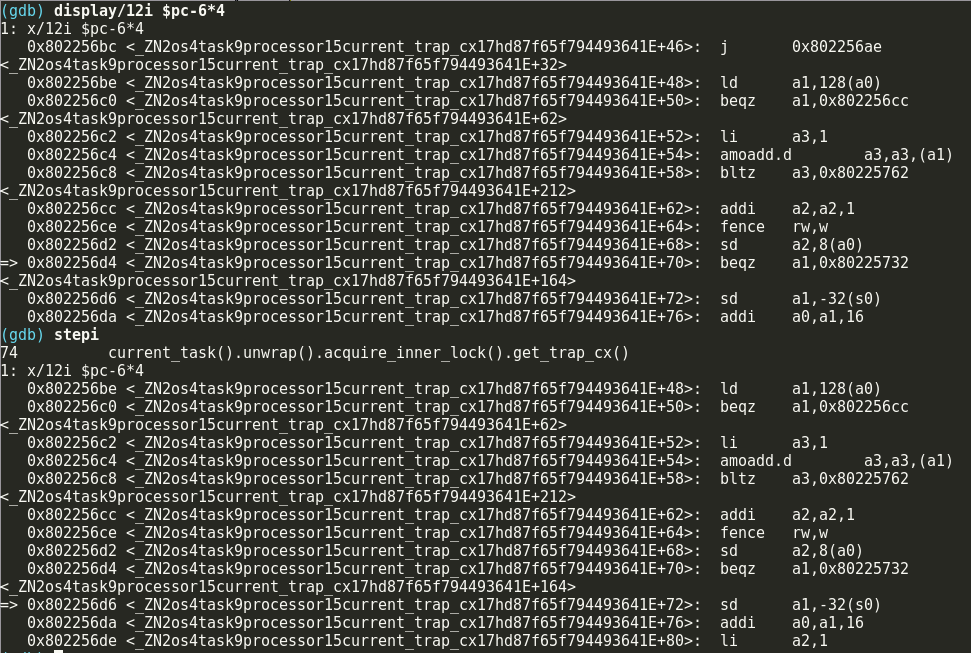
\includegraphics[width=\textwidth]{figures/02-02-display.png}
\caption{
	display
}
\label{fig:display}
\end{figure}

也可以info registers打印所有的寄存器

\begin{figure}[htb]
\centering
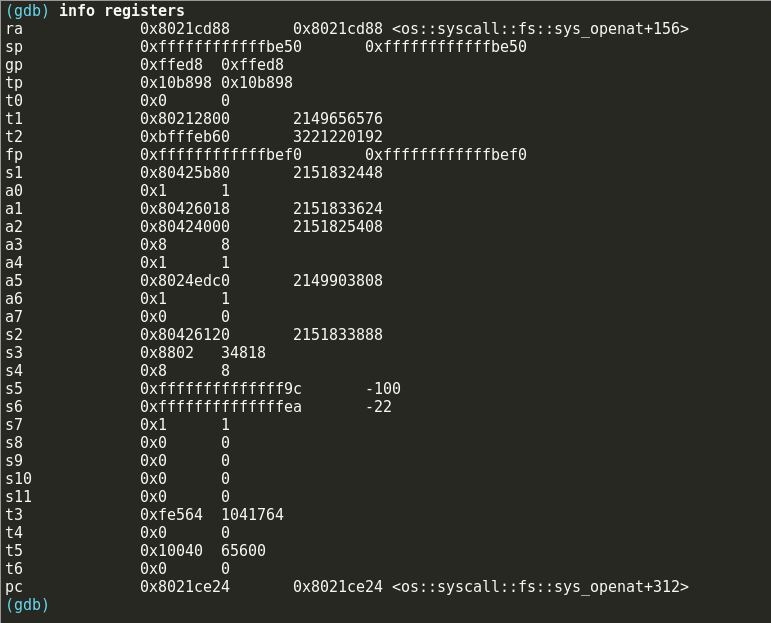
\includegraphics[width=\textwidth]{figures/02-02-info registers.png}
\caption{
	info registers
}
\label{fig:info registers}
\end{figure}

\textbf{自定义命令与脚本}

在使用GDB进行调试时,我们需要多次执行一些常见的指令。为了提高调试效率,我们可以使用define命令来定义自己的命令,简化重复操作。

下面我们来介绍如何定义一个自定义命令。首先,使用文本编辑器创建一个gdb脚本文件,例如mycommands.gdb。然后,在该文件中添加以下代码:

\begin{lstlisting}[language={Rust}, label={code:forktest},
	caption={forktest1.rs}]
	# 加载符号文件
	file target/riscv64gc-unknown-none-elf/debug/os
	add-symbol-file bash
	# 井号加入注释
	define mynext
	stepi
	info registers
	end
	# 添加bash的源代码
	dir 
\end{lstlisting}

这个自定义命令名为mynext,执行的操作包括执行下一条指令和显示所有寄存器的值。

接下来,启动GDB并加载定义的自定义命令。我们可以通过以下命令将mycommands.gdb文件加载到GDB中:

\begin{lstlisting}[language={Rust}, label={code:forktest},
	caption={forktest1.rs}]
	source mycommands.gdb
\end{lstlisting}

现在,我们可以在GDB中使用mynext命令来执行下一条指令并显示所有寄存器的值。只需在GDB提示符下输入“mynext”即可。

使用define自定义命令可以帮助我们快速地执行常见的调试操作,提高调试效率。 另外,其他的断点添加, 远程调试连接等命令也可以很方便地加入其中从而加速Debug过程。

在命令行下启动 GDB 并加载脚本时,可以使用 -x 或 –command 选项来指定要执行的脚本文件。该选项后跟要执行的脚本文件路径,如下所示:

\begin{lstlisting}[language={Rust}, label={code:forktest},
	caption={forktest1.rs}]
	# -x 选项指定了要执行的脚本文件路径,file_to_debug 则是要调试的目标程序的路径。
	gdb -x /path/to/script file_to_debug
	# 除了 -x 选项外,还可以使用 --init-command 选项指定要执行的初始化命令,该选项可以多次使用,每次指定一条命令,如下所示:
	gdb --init-command="set print pretty on" --init-command="set pagination off" file_to_debug
	# 上述命令中,--init-command 选项指定了要执行的初始化命令,可以多次使用,每次指定一条命令。
\end{lstlisting}


\subsection{git bisect——快速问题定位}
大家一定听过二分查找的算法, 如果我们发现某个Bug出现, 其实也可以通过二分查找定位到出错的版本。
git也自带了这个功能。使用git bisect, 我们可以在Git版本控制系统中进行二分查找,在版本历史中快速定位错误引入的位置。
\textbf{一般步骤}
我们以这些图文为例给出一个错误的处理
\begin{lstlisting}[language={Rust}, label={code:forktest},]
	$ git bisect start
	//运行 git bisect start 命令来启动一个二分查找会话。
	$ git bisect bad
	//用 git bisect bad 命令告诉 Git 当前版本存在问题。
	$ git bisect good HEAD~10
	//用 git bisect good 命令告诉 Git 一个知道没有问题的提交, 是这个提交的哈希值或分支名。git会给出估计的剩余步骤数
	Bisecting: 4 revisions left to test after this (roughly 2 steps)
	[f55d253527e3a72f730b06e6fbfe5e64f8594a27] fix: Change ELF related AuxV data alignment to repr(C), fixing the LPF.
	//Git 会自动切换到一个介于上述两个提交之间的提交,你需要在该提交上运行你的程序,检查问题是否存在。
	如果有问题,使用 git bisect bad 命令告诉 Git,否则使用 git bisect good 命令告诉 Git。
	你可以使用Git bisect run 切换提交后自动执行的命令(注意, git bisect run后仍然在原地, 这时候需要git bisect next才能进入下一个, 否则会冲突)
	Git 会根据你的反馈自动切换到下一个介于两个提交之间的提交,重复上述步骤,直到找到引入问题的提交。
	最后,使用 git bisect reset 命令退出二分查找会话。
\end{lstlisting}

\begin{figure}[htb]
	\centering
	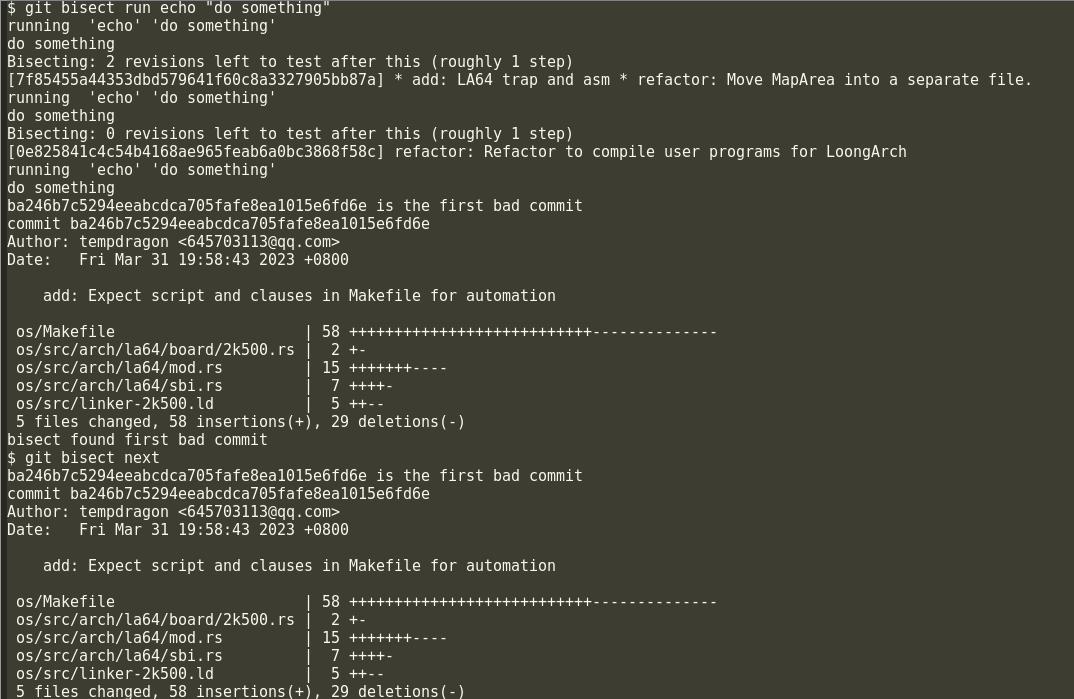
\includegraphics[width=\textwidth]{figures/02-02-运行实例.png}
	\caption{
		运行实例
	}
	\label{fig:运行实例}
\end{figure}
\textbf{log与冲突回撤}
如果发现某个提交被错误标记(比如bad被错误标记为good), 尝试
\begin{lstlisting}[language={Rust}, label={code:forktest},]
	git bisect bad
	你会得到以下错误:
	ba246b7c5294eeabcdca705fafe8ea1015e6fd6e was both good and bad
	
	$ git bisect log//导出日志:
	
	git bisect start
	# good: [ba246b7c5294eeabcdca705fafe8ea1015e6fd6e] add: Expect script and clauses in Makefile for automation
	git bisect good ba246b7c5294eeabcdca705fafe8ea1015e6fd6e
	# bad: [ba246b7c5294eeabcdca705fafe8ea1015e6fd6e] add: Expect script and clauses in Makefile for automation
	git bisect bad ba246b7c5294eeabcdca705fafe8ea1015e6fd6e
	//重定向到文件
	$ git bisect log > bis.log
	//考虑修改错误
	$ git bisect start
	会得到以下信息:
	# bad: [ba246b7c5294eeabcdca705fafe8ea1015e6fd6e] add: Expect script and clauses in Makefile for automation
	$ git bisect bad ba246b7c5294eeabcdca705fafe8ea1015e6fd6e
	
	$ git bisect replay bis.log
	//回复到之前的状态
\end{lstlisting}  

\section{NPUcore内核代码结构及内核构建目标}
\subsection{NPUcore内核代码树}
下面是NPUcore的内核代码树:
\begin{figure}[htb]
	\centering
	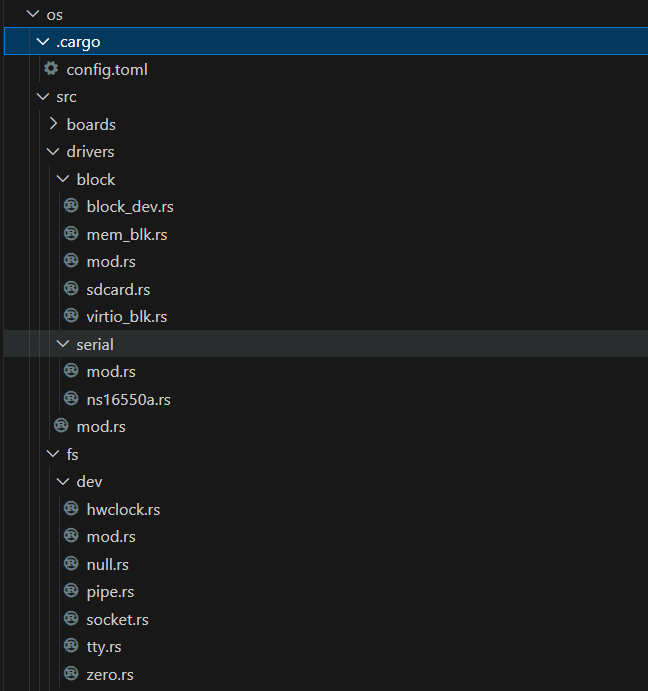
\includegraphics[width=\textwidth]{figures/02-03-内核代码树1.png}
	\caption{
		内核代码树1
	}
	\label{fig:内核代码树1}
\end{figure}

\begin{figure}[htb]
	\centering
	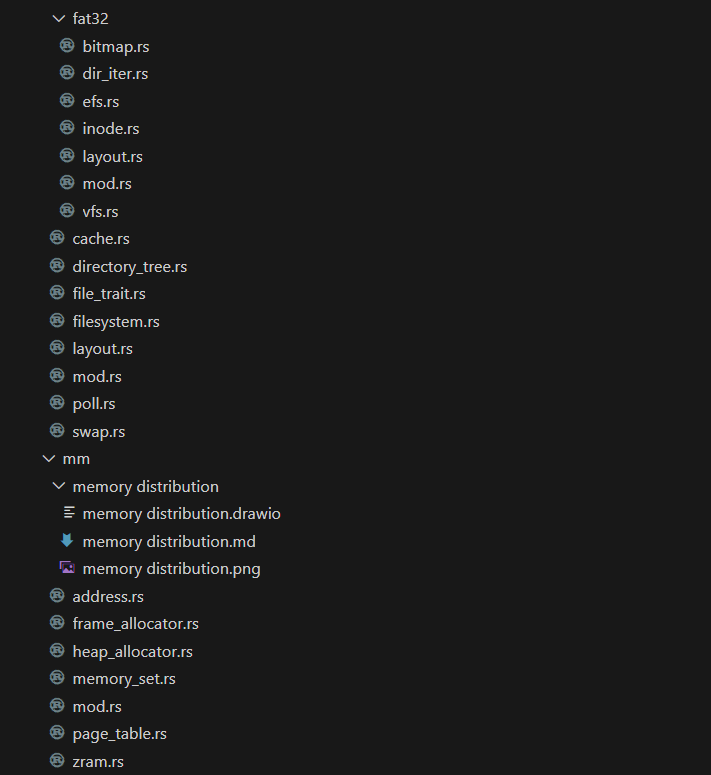
\includegraphics[width=\textwidth]{figures/02-03-内核代码树2.png}
	\caption{
		内核代码树2
	}
	\label{fig:内核代码树2}
\end{figure}

\begin{figure}[htb]
	\centering
	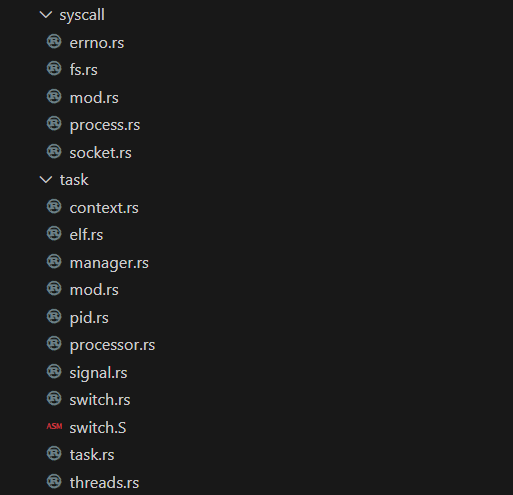
\includegraphics[width=\textwidth]{figures/02-03-内核代码树3.png}
	\caption{
		内核代码树3
	}
	\label{fig:内核代码树3}
\end{figure}

\begin{figure}[htb]
	\centering
	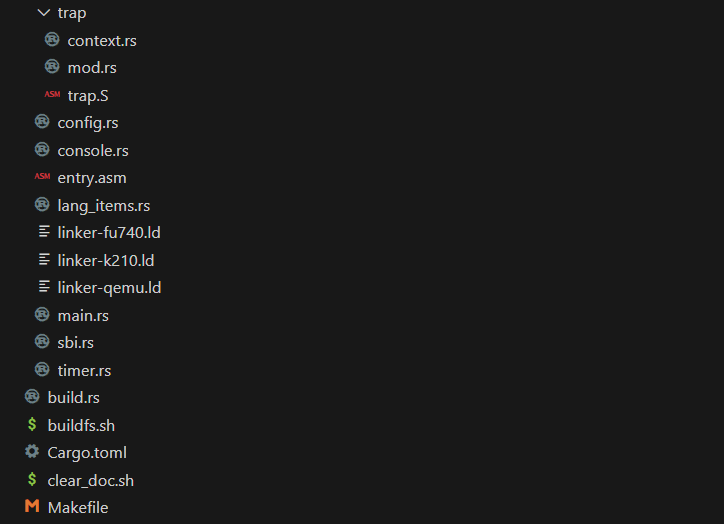
\includegraphics[width=\textwidth]{figures/02-03-内核代码树4.png}
	\caption{
		内核代码树4
	}
	\label{fig:内核代码树4}
\end{figure}


\subsection{NPUcore学习路线}
下面是我们为你准备的NPUcore的学习路线
\begin{figure}[htb]
	\centering
	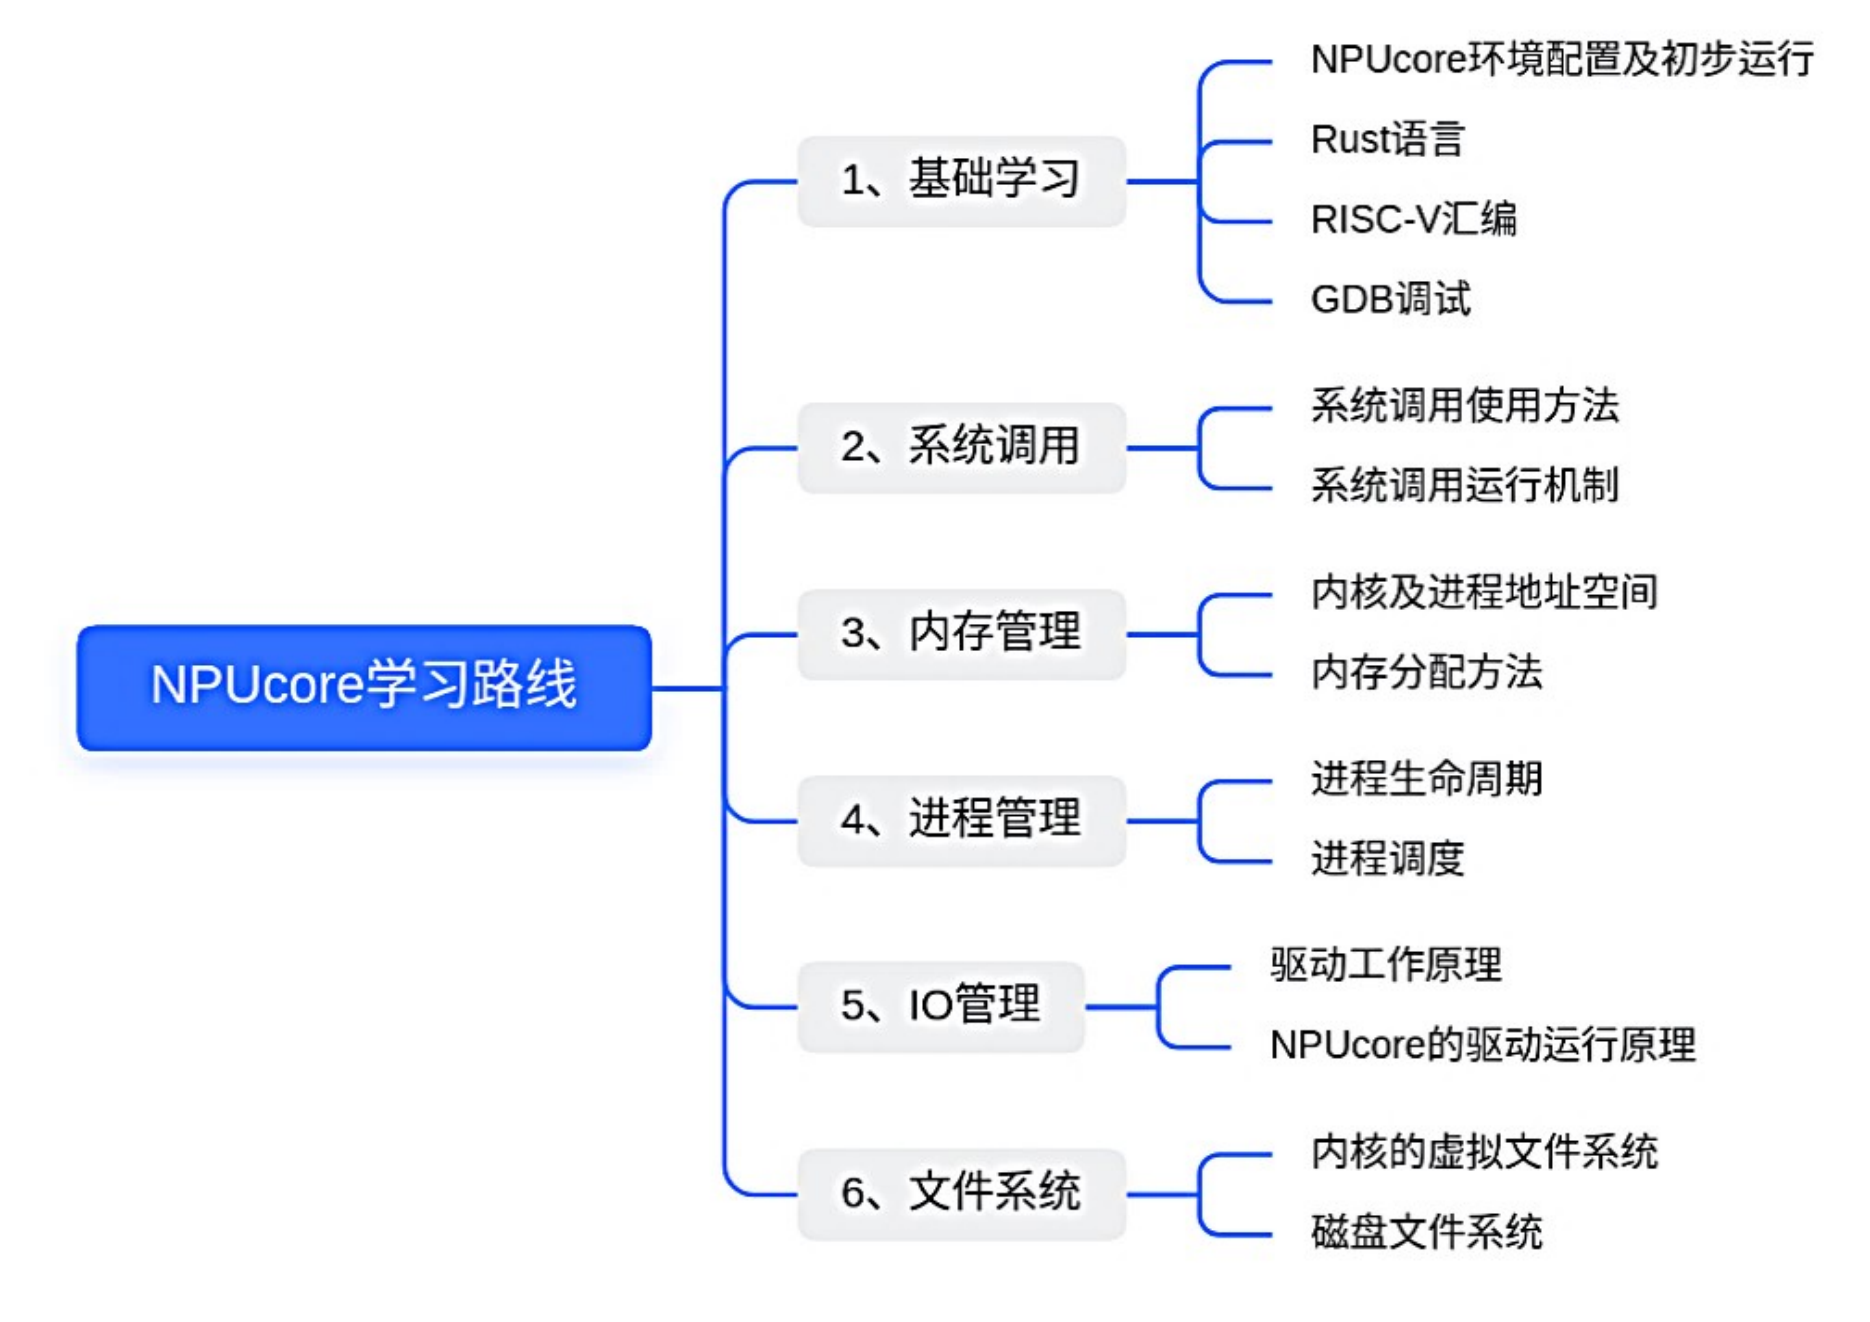
\includegraphics[width=\textwidth]{figures/02-03-NPUcore学习路线.png}
	\caption{
		NPUcore学习路线
	}
	\label{fig:NPUcore学习路线}
\end{figure}

希望你能渐渐的喜爱上操作系统~

\section{实验}

\chapter{LoongArch2K1000适配}

在NPUcore中,我们在os/arc/arch里对所有涉及硬件交互的组件均更新为LoongArch架构版本。
如代码片段\ref{code:content2}所示,我们的硬件设备约束,都放入arch中的la64文件夹,其中分为board,register,trap三个子文件夹。
在board中,2k1000.rs用于规定与2K1000开发板相关的串口宏(这个串口地址也是我们自己摸出来的,未找到任何官方说明)。
在register中,我们封装了base(基本寄存器),mmu(tlb相关),ras,timer的所有硬件相关寄存器。
在trap中,我们主要规定了内核态陷入方面所必须的类型与限制。
由于有关内存模块的适配最为艰难,因此,我们后面重点讲述这部分内容,同时也会提到基于2K1000-QEMU的适配。

\begin{lstlisting}[language={bash}, label={code:content2},
	caption={“os/arc/arch”目录树}]
    |-- la64
    |   |-- board
    |   |   |-- 2k1000.rs
    |   |-- config.rs
    |   |-- entry.asm
    |   |-- kern_stack.rs
    |   |-- la_libc_import.rs
    |   |-- laflex.rs
    |   |-- mod.rs
    |   |-- register
    |   |   |-- base
    |   |   |   |-- acpi.rs
    |   |   |   |-- badi.rs
    |   |   |   |-- badv.rs
    |   |   |   |-- crmd.rs
    |   |   |   |-- ecfg.rs
    |   |   |   |-- eentry.rs
    |   |   |   |-- era.rs
    |   |   |   |-- estat.rs
    |   |   |   |-- euen.rs
    |   |   |   |-- misc.rs
    |   |   |   |-- mod.rs
    |   |   |   |-- prcfg.rs
    |   |   |   |-- prmd.rs
    |   |   |   |-- rvacfg.rs
    |   |   |-- macros.rs
    |   |   |-- mmu
    |   |   |   |-- asid.rs
    |   |   |   |-- dmw.rs
    |   |   |   |-- mod.rs
    |   |   |   |-- pgd.rs
    |   |   |   |-- pwch.rs
    |   |   |   |-- pwcl.rs
    |   |   |   |-- stlbps.rs
    |   |   |   |-- tlbehi.rs
    |   |   |   |-- tlbelo.rs
    |   |   |   |-- tlbidx.rs
    |   |   |   |-- tlbrbadv.rs
    |   |   |   |-- tlbrehi.rs
    |   |   |   |-- tlbrelo.rs
    |   |   |   |-- tlbrentry.rs
    |   |   |   |-- tlbrera.rs
    |   |   |   |-- tlbrprmd.rs
    |   |   |-- mod.rs
    |   |   |-- ras
    |   |   |   |-- merrctl.rs
    |   |   |   |-- merrentry.rs
    |   |   |   |-- merrera.rs
    |   |   |   |-- mod.rs
    |   |   |-- timer
    |   |       |-- mod.rs
    |   |       |-- tcfg.rs
    |   |       |-- ticlr.rs
    |   |-- sbi.rs
    |   |-- switch.S
    |   |-- switch.rs
    |   |-- syscall_id.rs
    |   |-- time.rs
    |   |-- tlb.rs
    |   |-- trap
    |       |-- context.rs
    |       |-- mem_access.rs
    |       |-- mod.rs
    |       |-- trap.S
    |-- mod.rs
    
\end{lstlisting}

\section{LoongArch内存模块适配}

\subsection{内存地址映射布局}
LoongArch 的虚拟映射模式内存机理如下图:
\begin{figure}[htp]
    \centering
    \label{fig:mmu}
    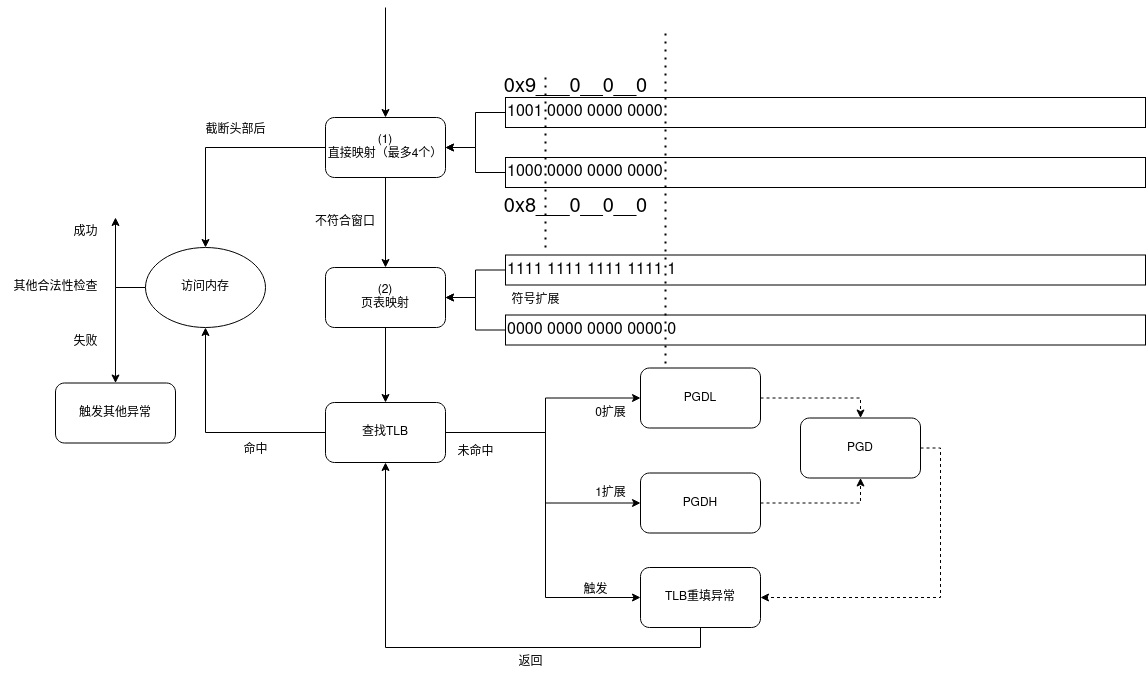
\includegraphics[width=0.8\linewidth]{figs/LA虚拟内存映射.png}
    \caption{LoongArch的虚拟映射模式}
\end{figure}
\begin{enumerate}
    \item 首先,检查是否符合直接映射窗口(通过DMW0~3四个CSR进行映射),
    如果其高4位相同则认为是符合,则将其他位数截断,作为物理地址访问。
    \item 其次,如果不是,则检查是否符号扩展,是则尝试查找 TLB,否则出发
    异常,在miss后,如果是1扩展则PGD为PGDH,0 扩展为 PGDL,
    然后触发TLB重填异常,ertn 返回后重新进行TLB查找。如果此时
    没有对应的TLB,则触发页无效异常。
    \item 此外, 对 DMW 的权限是: 0号和1号窗口是RWX, 2号和3号窗口是
    RW(不可执行)。 每个窗口可以单独设置自己的缓存一致性类型。

\end{enumerate}

由于 LoongArch 的特殊特性,NPUcore-IMPACT内存布局采取了和RISC-V下不同的方案:
\begin{enumerate}
    \item 对用户态,使用0扩展地址作为虚拟空间;
    \item 对内核态,用0扩展地址空间访问物理内存,然后对页表映射使用1扩展的地址。
\end{enumerate}
这样做可以用直接继承原版NPUcore的部分内存布局,无需为了利用 LA 的
直接映射窗口就大量修改代码,在物理地址上按位或大量的0x9000000090000000,减少代码出错空间。而且,这样可以利用直接映射减小恒等映射的开销,在上下文无需存储页表地址,可以直接切换地址空间。

\subsubsection{跳转}
从u-boot获得控制权时,引导程序提供了几个已经映射好的段: 0x9000
段 (一致可缓存), 和0x8000段 (无缓存直接访问内存), 前者使用 DMW1,
后者 DMW0(可能随u-boot版本不同而不同)。

由于地址空间中0段地址是不被映射的,因此需要某些方法先设置
DMW映射0段,再让PC跳转到该地址(NPUcore内核态的PC是在物
理地址上的)。为此, 我们的启动代码la64/entry.asm需要进行如下设计(如代码片段\autoref{code:entry})。

\begin{lstlisting}[language={riscv}, label={code:entry},
	caption={la64/entry.asm}]
_start:
    pcaddi      $t0,    0x0
    srli.d      $t0,    $t0,    0x30
    slli.d      $t0,    $t0,    0x30    # 位移删去物理地址
    addi.d      $t0,    $t0,    0x11    # 计算当前的窗口CSR值
    csrwr       $t0,    0x181           # 上面代码保证窗口DMW0写入切换后不会被覆盖,所以先将DMW1设为当前段
    sub.d       $t0,    $t0,    $t0
    addi.d      $t0,    $t0,    0x11    # 计算0段DMW的值
    csrwr       $t0,    0x180           # 设置0段DMW的值
    pcaddi      $t0,    0x0
    slli.d      $t0,    $t0,    0x10
    srli.d      $t0,    $t0,    0x10
    jirl        $t0,    $t0,    0x10    # 跳0段的下一条指令
    # The barrier
    sub.d       $t0,    $t0,    $t0
    csrwr       $t0,    0x181           # 写入DMW1, 清零DMW1
    sub.d       $t0,    $t0,    $t0     # 加载boot_stack_top
    la.global $sp, boot_stack_top       # 跳转到rust_main
    bl          rust_main
\end{lstlisting}
注意这里没有使用\$t0=\$zero是因为在QEMU虚拟机下, 某些时候似
乎\$zero寄存器会被赋值为0(GDB提示), 因此使用手工计算的 \$t0=0。
这里先设置映射窗口, 而不是计算完0段的DMW控制寄存器数值后直接
覆盖到DMW0的原因是:如果当前PC的地址处在DMW0而非DMW1的区段内, 覆盖DMW0后PC的地址就会成为非法地址。
跳转必然发生在映射了新的区段号后,因此要先将当前的区段保存到DMW1, 然后再进行对DMW0的配置,
从而确保至少有一个DMW是PC当前的地址。

\subsection{不对齐读写问题}
当前开源的LLVM的LoongArch后端不支持生成严格对齐
的代码, 因此也导致依赖LLVM后端进行代码生成的Rustc无法编译出可
以在开发板上正常运行的代码, 这也就要求我们对NPUcore的不对齐异常手动处理。

虽然 QEMU 支持不对齐读写, 但是开发板是无法支持不对齐读写的.
如果要在 QEMU 上支持不对齐读写的检测和不对齐读写的报错, 需要开启
环境变量 DEBUG_UNALIGN=1, 否则会忽略所有的不对齐读写异常。
具体的启动命令是:DEBUG_UNALIGN=1 DEBUG_GMAC_PHYAD=0 DEBUG_MYNAND=cs=0,id=0x2cda DEBUG_MYSPIFLASH=gd25q128 \$QEMU。

如果将来LoongArch的LLVM完成了严格对齐读写的修复, 则应当可
以用target-feature开启编译器的选项:
\begin{lstlisting}[language={rust}, label={code:entry},
	caption={la64/entry.asm}]
[target.loongarch64-unknown-linux-gnu]
rustflags = ["-Ctarget-feature=-unaligned-access",
"-Clink-arg=-Tsrc/linker.ld", "-Clink-arg=-nostdlib", "-Clink-arg=-static"]
\end{lstlisting}
这个问题在C语言的GCC下是不存在的, 因此, 理论上在Rust编写
的操作系统上, 当前会由于不对齐读写存在性能瓶颈。 为了解决这个问题, 我
们需要在内核态手动模拟不对齐读写指令的执行。

内核态的不对齐异常只出现在栈上, 因为静态数据和堆上的数据结构是对齐的, 而NPUcore-LA的内核堆则是从栈上分配
的, 只有在ELF加载阶段有部分只读临时的内核页表映射。 因此, 只需要保
存内容后, 对进行逐字节解读取即可。具体来说, 为了节省内容恢复的空间, 我们直接对kernel trap的设计为:
\begin{enumerate}
    \item 内容保存不需要单独建立一个位置, 直接将寄存器上下文保存在栈上,
    因为内核的不对齐读写异常是发生在执行时, 所以直接视为一个单独
    的函数调用即可。
    \item 指令解码使用。
\end{enumerate}

内容保存的代码如下:
\begin{lstlisting}[language={riscv}, label={code:trap},
	caption={la64/trap/trap.S}]
    __kern_trap:
    # Keep the original $sp in SAVE
    csrwr $sp, CSR_SAVE    
    csrrd $sp, CSR_SAVE
    # Now move the $sp lower to push the registers
    addi.d $sp, $sp, -256
    # Align the $sp
    srli.d  $sp, $sp, 3
    slli.d  $sp, $sp, 3
    # now sp->*GeneralRegisters in kern space, CSR_SAVE->(the previous $sp)

    SAVE_GP 1 # Save $ra
    SAVE_GP 2 # Save $tp

    # skip r3(sp)
    .set n, 4
    .rept 28
        SAVE_GP %n
        .set n, n+1
    .endr
    .set n, 0
    csrrd $t0, CSR_ERA
    st.d $t0, $sp, 0

    move $a0, $sp
    csrrd $sp, CSR_SAVE
    st.d $sp, $a0, 3*8
    move $sp, $a0

    bl trap_from_kernel

    ld.d  $ra, $sp, 0
    csrwr $ra, CSR_ERA
    LOAD_GP 1
    LOAD_GP 2

    # skip r3(sp)
    .set n, 4
    .rept 28
        LOAD_GP %n
        .set n, n+1
    .endr
    .set n, 0
    
    csrrd $sp, CSR_SAVE
    ertn
\end{lstlisting}


读写的关键代码如下:
\begin{lstlisting}[language={rust}, label={code:trap},
	caption={la64/trap/trap.S}]
if op.is_store() {
                    let mut rd = gr[ins.get_rd_num()];
                    for i in 0..sz {
                        unsafe { ((addr + i) as *mut u8).write_unaligned(rd as u8) };
                        rd >>= 8;
                    }
                } else {
                    let mut rd = 0;
                    for i in (0..sz).rev() {
                        rd <<= 8;
                        let read_byte =
                            (unsafe { ((addr + i) as *mut u8).read_unaligned() } as usize);
                        rd |= read_byte;
                        //debug!("{:#x}, {:#x}", rd, read_byte);
                    }
                    if !op.is_unsigned_ld() {
                        match sz {
                            2 => rd = (rd as u16) as i16 as isize as usize,
                            4 => rd = (rd as u32) as i32 as isize as usize,
                            8 => rd = rd,
                            _ => unreachable!(),
                        }
                    }
                    gr[ins.get_rd_num()] = rd;
                }
                gr.pc += 4;
\end{lstlisting}

注意这里的rev是必须的, 因为LoongArch是小端机器, 所以高字节的先读才能被或到低位。
理论上, 还存在更快的办法, 就是判断是否跨整$2^{n}$字节, 如果不跨
过, 则用汇编选择对应字节的内容, 否则就读入两寄存器(128bits)再取各自
需要的部分组合成一个寄存器的值. 但由于其实现较为复杂, 所以我们考虑在决赛时采用。

\subsection{TLB refill与页表结构}
\subsubsection{TLB重填异常}
\begin{figure}
    \centering
    \label{fig:TLB}
    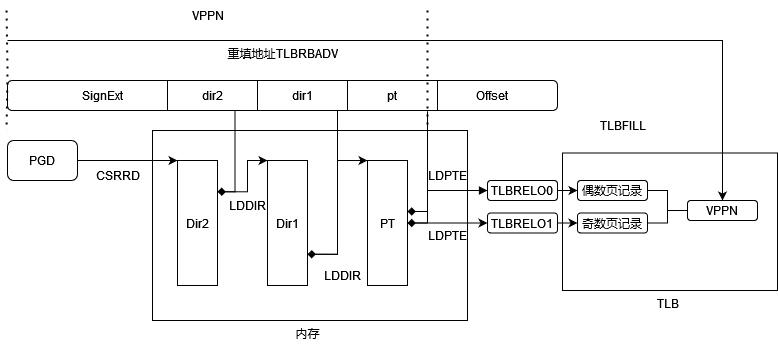
\includegraphics[width=1\linewidth]{figs/TLB重填.png}
    \caption{TLB重填}
\end{figure}
如图\autoref{fig:TLB},一旦在虚拟地址模式中被判定为页表映射的地址, 发生 TLB miss, 就会
触发 TLB 重填异常。LoongArch 目前是手动重填 TLB 的。其重填的一般
流程如下:
\begin{enumerate}
    \item 硬件提供页表地址PGD。
    \begin{enumerate}[label=$(\mathbf{\arabic*})$]
        \item  LoongArch 有两个页表 PGDL 和 PGDH,分别对应符号扩展的全1段和0段。
        \item  如果触发重填的地址来自 0 段, 则重填的页表 PGD 此时等于PGDL, 否则 PGD 此时等于 PGDH。这样一来, 页表实际上分为了高地址和低地址页表, 可以用作不同的功能。
    \end{enumerate}
    \item 硬件触发TLB异常,跳转到TLBRENTRY CSR所指向的地址。
    \item 操作系统会响应异常,通过读取PGD状态控制寄存器, 获取最高一级页表目录。
    \item 根据虚拟地址计算出对应的物理页框号。然后在主存中查找该物理页
    框的对应页表项,然后返回该页表项的物理地址. 为了加速页表重填,
    LoongArch 提供了下列特性:
    \begin{enumerate}[label=$(\mathbf{\arabic*})$]
        \item LoongArch 的 TLB 以双页形式组织,目的是减少重填次数。具
        体来说,LoongArch 的 TLB 的索引单位是 VPPN(Virtual Page
        Pair Number),为虚拟页号去掉最第一位。每个 VPPN 对应 VPN
        为 VPPN×2+VPN[12] 的一对奇数页和偶数页两页的物理地址。
        考虑到 TLB 重填的局部性,这样最多可以减少一半的 TLB 重
        填。
        \item LoongArch 提供 LDDIR 和 LDPTE 两种指令进行页表遍历,通
        过 TLBRBADV 寄存器提供重填的虚拟地址,并以此为基础获得
        各级页表的索引号。LDDIR 是用于给定非末级页表起始地址,求
        取本级页表项(或者说下一级页表起始地址),其格式为 (其中
        imm 为页表级数。以 rj 为页表起始地址,rd 为目的寄存器。):
        LDDIR rd, rj, imm。
    \end{enumerate}
    \item 返回页表项后,处理器将该对页表项用 TLBFILL 写入 TLB 中,以便
    下次使用该虚拟地址时,能够直接从 TLB 中获取物理地址信息,而不
    需要再次触发 TLB 重填。在 TLB 更新后,处理器会重新执行之前的
    指令或内存访问操作,这次操作可以直接从 TLB 中获取到物理地址。
\end{enumerate}

\subsubsection{LoongArch的页表结构}
官方手册对 LoongArch 的项目并没有清晰的叙述, 其中存在部分不明
确的地方。 具体来说(如图\autoref{fig:page}), 除了大页之外, LoongArch 并不规定页目录的页表项
格式, 所以其实际上是未定义的。
\begin{figure}
    \centering
    \label{fig:page}
    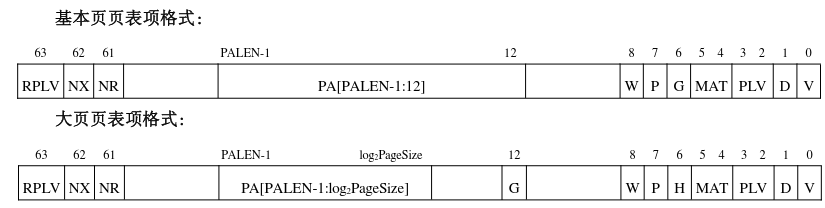
\includegraphics[width=1\linewidth]{figs/页表格式.png}
    \caption{LA页表格式}
\end{figure}
而上文提到的 LDDIR 和 LDPTE 并不检查目录项合法性, 且对非法的
页表项仍会继续寻址, 因此, 对目录项需要有手工的检测或者非法目录项的
处理方法。最简单的方法是直接模拟其他 RISC 架构的页表处理方式, 直接用汇编
代码对各层页表项进行处理。 首先, 页表是一棵前缀树, 其部分没有被映射
的节点是空的, 因此如果直接使用上述的 LDPTE 和 LDDIR, 由于其只是单
纯的将异常地址的对应段取出作相加, 因此对空的地址会计算出错误的地址,
而不是和其他 RISC 一样触发异常。 因此, 非最底层页表的叶结点 (空表项)
必须要手工判断, 并对其错误的表项, 填写无读写权限的 TLB 表项。

\begin{lstlisting}[language={riscv}, label={code:refill},
	caption={TLB refill}]
    csrwr  $t0, 0x8b
    csrrd  $t0, 0x1b
    lddir  $t0, $t0, 3
    andi   $t0, $t0, 1
    beqz   $t0, 1f

    csrrd  $t0, 0x1b
    lddir  $t0, $t0, 3
    addi.d $t0, $t0, -1
    lddir  $t0, $t0, 1
    andi   $t0, $t0, 1
    beqz   $t0, 1f
    csrrd  $t0, 0x1b
    lddir  $t0, $t0, 3
    addi.d $t0, $t0, -1
    lddir  $t0, $t0, 1
    addi.d $t0, $t0, -1

    ldpte  $t0, 0
    ldpte  $t0, 1
    csrrd  $t0, 0x8c
    csrrd  $t0, 0x8d
    csrrd  $t0, 0x0
2:
    tlbfill
    csrrd  $t0, 0x89
    srli.d $t0, $t0, 13
    slli.d $t0, $t0, 13
    csrwr  $t0, 0x11
    tlbsrch
    tlbrd
    csrrd  $t0, 0x12
    csrrd  $t0, 0x13
    csrrd  $t0, 0x8b
    ertn
1:
    csrrd  $t0, 0x8e
    ori    $t0, $t0, 0xC
    csrwr  $t0, 0x8e

    rotri.d $t0, $t0, 61
    ori    $t0, $t0, 3
    rotri.d $t0, $t0, 3

    csrwr  $t0, 0x8c
    csrrd  $t0, 0x8c
    csrwr  $t0, 0x8d
    b      2b
\end{lstlisting}

代码片段\autoref{code:refill}实现了以下功能:
\begin{enumerate}
    \item 逐层读取页表项, 如果没到最后一层, 检查读取到的页表项的合法性。合法则继续读取下一级页表项;非法则准备填入 0 页表项, 表示该页非法。
    \item 填入 0 页表项或者读取最后一层页表项结束后, 将页表大小填写为4KiB, 然后向 TLB 填入 0 地址, 表示该地址不合法。注意, 这段代码
    有 2 个需要注意的细节:
    \begin{enumerate}[label=$(\mathbf{\arabic*})$]
        \item 由于该段代码使用的 csrwr 指令在 LoongArch 下的语义是交换
        CSR 和寄存器的内容, 而非简单地将寄存器内容写入, 因此在向
        两个相同结构的 CSR 填入某个相同数值的时候, 我们需要重新读
        取之前的目的寄存器, 然后重新写入才能正确处理结果。
        \item 之所以需要对 TLB Refill exception Entry HIgh-order bits (TLBREHI)(0x8e) 的状态控制寄存器填入 0, 是因为该地址内包括页
        长度相关的域, 但该地址原本是由 ldpte 填写, 为了防止手动填写
        TLB 项导致未定义行为 (填入错误的 TLB 或虚拟机报错), 我们
        需要先对该页填写 0 地址。
    \end{enumerate}
\end{enumerate}
\section{LoongArch的启动步骤}
首先是 NPUcore 的主函数:
\begin{lstlisting}[language={rust}, label={code:refill},
	caption={os/src/main.rs}]
#[no_mangle]
pub fn rust_main() -> ! {
    println!("[kernel] NPUcore-IMAPCT!!! ENTER!");
    bootstrap_init();
    mem_clear();
    console::log_init();
    move_to_high_address(); \\ img move in kernel
    println!("[kernel] Console initialized.");
    mm::init();

    machine_init();
    println!("[kernel] Hello, world!");

    //machine independent initialization
    fs::directory_tree::init_fs();
    task::add_initproc();

    // note that in run_tasks(), there is yet *another* pre_start_init(),
    // which is used to turn on interrupts in some archs like LoongArch.
    task::run_tasks();
    panic!("Unreachable in rust_main!");
}
\end{lstlisting}
我们可以看到, 除了 bootstrap_init() 和 machine_init(), 其他都是平台无关
的, 因此这里主要介绍平台相关的启动流程。其中, machine_init() 的发生在 mm::init() 后。
\begin{lstlisting}[language={rust}, label={code:refill},
	caption={os/src/arch/la64/mod.rs - bootstrap\_init}]
    pub fn bootstrap_init() {
        /* if CPUId::read().get_core_id() != 0 {
         *     loop {}
         * } */
        ECfg::empty()
            .set_line_based_interrupt_vector(LineBasedInterrupt::TIMER)
            .write();
        EUEn::read().set_float_point_stat(true).write();
        // Timer & other Interrupts
        TIClr::read().clear_timer().write();
        TCfg::read().set_enable(false).write();
        CrMd::read()
            .set_watchpoint_enabled(false)
            .set_paging(true)
            .set_ie(false)
            .write();
    
        // Trap/Exception Hanlder initialization.
        set_kernel_trap_entry();
        set_machine_err_trap_ent();
        TLBREntry::read().set_addr(srfill as usize).write();
    
        // MMU Setup
        DMW2::read()
            .set_plv0(true)
            .set_plv1(false)
            .set_plv2(false)
            .set_plv3(false)
            .set_vesg(SUC_DMW_VESG)
            .set_mat(MemoryAccessType::StronglyOrderedUnCached)
            .write();
        DMW3::empty().write();
        //DMW1::empty().write();
    
        STLBPS::read().set_ps(PTE_WIDTH_BITS).write();
        TLBREHi::read().set_page_size(PTE_WIDTH_BITS).write();
        PWCL::read()
            .set_ptbase(PAGE_SIZE_BITS)
            .set_ptwidth(DIR_WIDTH)
            .set_dir1_base(PAGE_SIZE_BITS + DIR_WIDTH)
            .set_dir1_width(DIR_WIDTH) // 512*512*4096 should be enough for 256MiB of 2k1000.
            .set_dir2_base(0)
            .set_dir2_width(0)
            .set_pte_width(PTE_WIDTH)
            .write();
        PWCH::read()
            .set_dir3_base(PAGE_SIZE_BITS + DIR_WIDTH * 2)
            .set_dir3_width(DIR_WIDTH)
            .set_dir4_base(0)
            .set_dir4_width(0)
            .write();
    
        println!("[kernel] UART address: {:#x}", UART_BASE);
        println!("[bootstrap_init] {:?}", PRCfg1::read());
    }    
\end{lstlisting}
我们可以看到, 在上面的启动过程中, 龙芯实际上中断要触发有几个使
能层:
\begin{enumerate}
    \item 中断本身的使能, 来自 ECfg。
    \item 中断源的使能 (如果存在), e.g. 时钟中断来自 TCfg。
    \item CrMd: 当前模式寄存器的中断使能。
    \item 最后是 Trap Handler 相关的设置和内存相关的初始化。
\end{enumerate}
对于机器相关初始化, 主要是初始化时钟相关的内容。
\begin{lstlisting}[language={rust}, label={code:refill},
	caption={os/src/arch/la64/mod.rs - machine\_init}]
    pub fn machine_init() {
    // remap_test not supported for lack of DMW read only privilege support
    trap::init();
    get_timer_freq_first_time();
    /* println!(
     *     "[machine_init] VALEN: {}, PALEN: {}",
     *     cfg0.get_valen(),
     *     cfg0.get_palen()
     * ); */
    for i in 0..=6 {
        let j: usize;
        unsafe { core::arch::asm!("cpucfg {0},{1}",out(reg) j,in(reg) i) };
        println!("[CPUCFG {:#x}] {}", i, j);
    }
    for i in 0x10..=0x14 {
        let j: usize;
        unsafe { core::arch::asm!("cpucfg {0},{1}",out(reg) j,in(reg) i) };
        println!("[CPUCFG {:#x}] {}", i, j);
    }
    println!("{:?}", Misc::read());
    println!("{:?}", RVACfg::read());
    println!("[machine_init] MMAP_BASE: {:#x}", MMAP_BASE);
    trap::enable_timer_interrupt();
}
\end{lstlisting}
之所以将这些内容放到这里, 是因为 LoongArch 下的恒等时钟频率是可以通过指令获取的, 
如果因此我们获取后存入静态数据区域, 所以需要在
bss 段被清 0 后才开始处理时钟相关中断。
\section{系统调用机制与中断}
\section{实验}

\chapter{内存管理}
\section{RISC-V页表硬件}

为了提高系统对物理内存的动态使用效率,隔离各应用的物理内存空间以保证应用间的安全性,我们对硬件层面的物理内存空间进行了一层抽象,建立了虚拟地址空间到物理内存空间的映射。从此,每个应用程序都享有独属于自己的,且足够庞大 (一般来说) 的存储空间,而不用与其他应用程序“抢占”资源。而将每个应用的逻辑地址空间分配到实际的物理内存空间这一任务,正是由操作系统来负责。

在分页内存管理中,操作系统通过“页表”来实现虚实内存映射机制,这是我们本章介绍的重点内容。同时,我们也可以使用页表来实现许多“有趣”的功能,例如将不同的地址空间映射至同一块物理内存空间,以实现共享内存;或是使用未映射的页面来保护内核和用户栈等等。

\subsection{虚拟地址与物理地址}

\subsubsection{地址的格式及关系}

如之前提到,实现虚拟地址到物理地址的映射,也就是页表的实现是我们本章的重点。不过在具体介绍页表之前,我们先来介绍我们所要维护的对象——虚拟地址与物理地址。

在Npucore中,虚拟地址空间和物理地址空间均采用页式管理,且每个页面的大小为 4KiB ($2^{12}$B)。如此一来,一个虚拟页面中的数据正好对应存储在一个物理页帧上,便于管理。根据页面大小的规定可知,每个页面需要使用12位字节地址来进行页内索引。根据页式管理的知识,我们将虚拟地址和物理地址均分成两部分:它们的低12位,即[11:0]被称为页内偏移 (Page Offset),它描述一个地址指向的字节在其所在页面中的相对位置。在SV39分页模式下,我们规定虚拟地址一共39位,则虚拟地址的高27位,即[38:12]为它的虚拟页号VPN (Virtual Page Number);我们规定物理地址一共56位,则物理地址的高44位,即[55:12]为它的物理页号PPN (Physical Page Number)。因此,地址的格式如图4-1所示:

\begin{figure}[h]
	\centering
	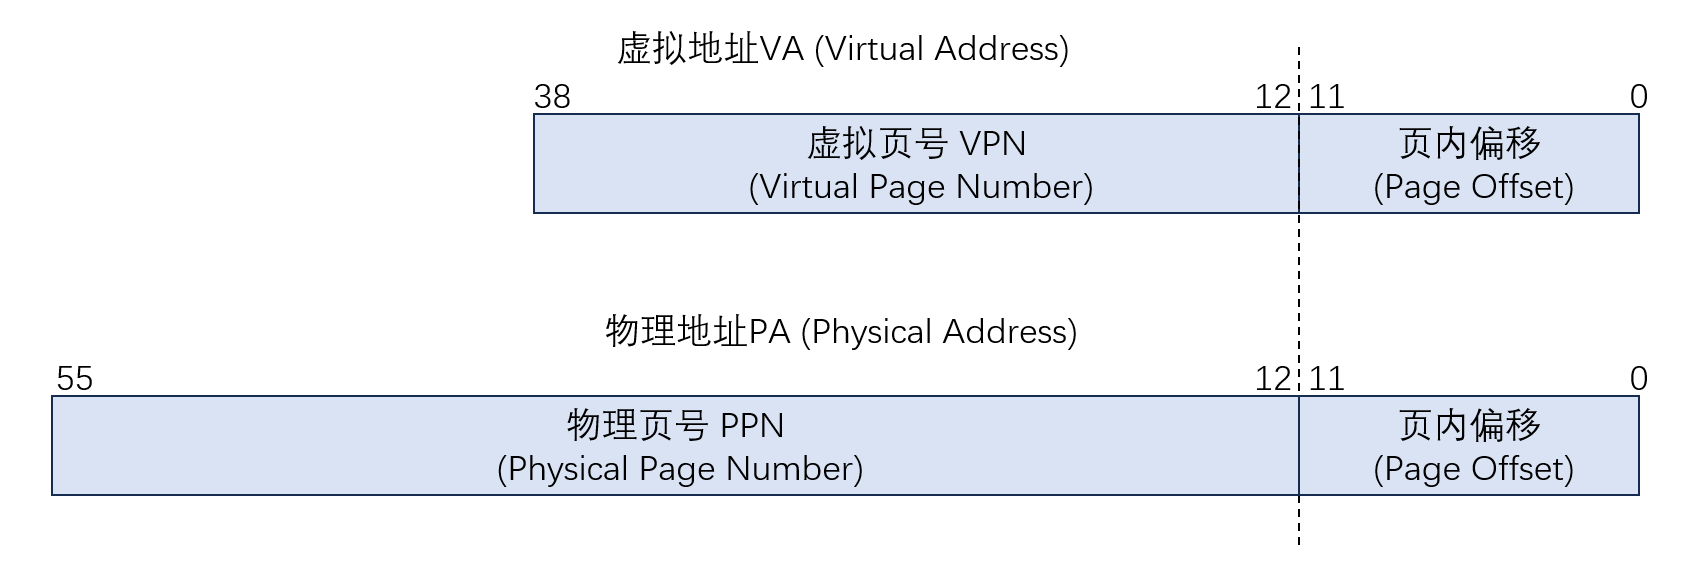
\includegraphics[width=.80\textwidth]{figures/04-01-虚拟地址与物理地址的格式.png}
	\caption{虚拟地址与物理地址的格式}
\end{figure}\FloatBarrier

回到我们的重点——地址转换。页式管理下,地址的转换是以页为单位进行的。也就是说,地址转换前后地址的页内偏移部分是不变的。因此,我们实际上要完成的操作是:从虚拟地址中取出27位虚拟页号,在页表中查询其对应的物理页号(若存在),最后将这27位虚拟页号映射得到的44位的物理页号与虚拟地址的12位页内偏移按序拼接到一起,就得到了56位的物理地址,完成了地址转换的过程。

\subsubsection{地址的数据结构抽象}

物理地址共有56位,这是由RISC-V的硬件设计人员决定的。但在64位的架构上,虚拟地址长度确实应该和位宽一致,为64位。不过在SV39分页模式下,虚拟地址只有低39位是有实际意义的。SV39分页模式规定64位虚拟地址的高25位必须和第38位相同,否则内存管理单元(MMU)会直接认定它是一个不合法的虚拟地址。通过这个检查之后,MMU再取出低39位尝试将其转化为一个56位的物理地址。同样,为了易于数据结构的实现,我们也将物理地址以64位进行封装。具体的实现如下:

\begin{lstlisting}[language={Rust}, label={code:address},
		caption={os/src/mm/address.rs}]
// Definitions
#[repr(C)]
#[derive(Copy, Clone, Ord, PartialOrd, Eq, PartialEq)]
pub struct PhysAddr(pub usize);

#[repr(C)]
#[derive(Copy, Clone, Ord, PartialOrd, Eq, PartialEq)]
pub struct VirtAddr(pub usize);
	
#[repr(C)]
#[derive(Copy, Clone, Ord, PartialOrd, Eq, PartialEq)]
pub struct PhysPageNum(pub usize);

#[repr(C)]
#[derive(Copy, Clone, Ord, PartialOrd, Eq, PartialEq)]
pub struct VirtPageNum(pub usize);
\end{lstlisting}

上面分别给出了物理地址PA、虚拟地址VA、物理页号PPN、虚拟页号VPN的类型声明,它们都是元组式结构体,可以看成usize的一种简单包装。我们刻意将它们各自抽象出不同的类型而不是都使用与RISC-V 64硬件直接对应的usize基本类型,是为了在Rust编译器的帮助下,通过多种安全且方便的类型转换来构建页表。

实现这些地址信息类型与usize类型之间的相互转换,需要使用From<T> trait (同时实现了Into<T> trait)。这里我们以PPN为例,介绍其与usize类型的转换(其余三种地址信息类型PA、VA、VPN的实现均一致,仅有类型声明的差异)。对usize类型实现以下trait,使我们可以使用usize类型数据生成一个PhysPageNum类型的数据:

\begin{lstlisting}[language={Rust}, label={code:address},
	caption={os/src/mm/address.rs}]
impl From<usize> for PhysPageNum {
	fn from(v: usize) -> Self {
		Self(v)
	}
}
\end{lstlisting}

反过来,同样对PhysPageNum类型实现该trait,使我们可以使用PhysPageNum类型数据生成一个usize类型的数据:

\begin{lstlisting}[language={Rust}, label={code:address},
	caption={os/src/mm/address.rs}]
impl From<PhysPageNum> for usize {
	fn from(v: PhysPageNum) -> Self {
		v.0
	}
}
\end{lstlisting}

至此,我们实现了地址信息类型与usize类型的相互转换。注意到,从地址信息变量(以PPN为例)得到它的usize类型的更简便方法是直接ppn.0。

同时,我们也支持地址类型与页号类型的相互转换。需要注意的是,从页号到地址的转换只需左移12位即可;而地址转换至页号则必须保证它与页面大小对齐(即页内偏移为0),若不对齐,则需要先进行取整。接下来以物理地址与物理页号的转换为例:

首先介绍地址的取整:

\begin{lstlisting}[language={Rust}, label={code:address},
	caption={os/src/mm/address.rs}]
impl PhysAddr {
	pub fn floor(&self) -> PhysPageNum {
		PhysPageNum(self.0 / PAGE_SIZE)
	}
	pub fn ceil(&self) -> PhysPageNum {
		PhysPageNum((self.0 + PAGE_SIZE - 1) / PAGE_SIZE)
	}
}
\end{lstlisting}

floor为下取整方法,而ceil为上取整方法。其中,PAGE\_SIZE为4096,表示每个页面的大小。

接下来介绍地址与页号的转换,我们同样是实现From<T> trait:

\begin{lstlisting}[language={Rust}, label={code:address},
	caption={os/src/mm/address.rs}]
impl PhysAddr {
	pub fn page_offset(&self) -> usize { self.0 & (PAGE_SIZE - 1) }
}

impl From<PhysAddr> for PhysPageNum {
	fn from(v: PhysAddr) -> Self {
		assert_eq!(v.page_offset(), 0);
		v.floor()
	}
}

impl From<PhysPageNum> for PhysAddr {
	fn from(v: PhysPageNum) -> Self { Self(v.0 << PAGE_SIZE_BITS) }
}
\end{lstlisting}

其中,PAGE\_SIZE\_BITS为12,表示页内偏移的位宽。

至此,我们对地址信息类型的实现已经有了基本的掌握。

\subsection{页表项}

\subsubsection{页表项格式及含义}

在上面的内容中其实我们已经认识到,虚实地址转换的流程核心就是:使用虚拟页号作为索引在页表中查询到对应的物理页号。若把页表比作一个货架,则虚拟页号就是商品的编号,我们通过这个编号寻找到对应的商品,而这个商品就存储着我们需要的物理地址信息。“这个商品”指的就是页表项。

SV39分页模式下,页表项是一个8字节的比特序列,其结构如图4-2所示:

\begin{figure}[h]
	\centering
	\includegraphics[width=.80\textwidth]{figures/04-02-页表项的格式.png}
	\caption{页表项的格式}
\end{figure}\FloatBarrier

可见,[63:54]这10位是保留位,被忽略;[53:10]这44位是物理页号;而最低的10位[9:0]则是标志位。标志位实际上控制了应用对其地址空间中每个虚拟页面的访问权限,他们的具体含义如下:

\begin{itemize}
	\item [$\bullet$]
	V(Valid):有效位。仅当V为1时,该页表项合法;
	\item [$\bullet$]
	R(Read)/W(Write)/X(eXecute):分别表示索引到这个页表项的对应虚拟页面是否允许读/写/执行;
	\item [$\bullet$]
	U(User):表示索引到这个页表项的对应虚拟页面是否在CPU处于U特权级的情况下允许访问;
	\item [$\bullet$]
	G(Global):全局标志。为1时表明该页面为全局页面;
	\item [$\bullet$]
	A(Accessed):处理器使用此位来记录自页表项上的这一位被清零后,其对应虚拟页面是否被访问过;
	\item [$\bullet$]
	D(Dirty):处理器使用此位来记录自页表项上的这一位被清零后,其对应虚拟页面是否被修改过;
	\item [$\bullet$]
	RSW(Reserved for Supervisor softWare):保留位。该部分被处理器忽略,软件可以使用。	
\end{itemize}

总之,页表项不仅存储了物理地址信息,还存储了一组标志位用于对虚拟页面的权限控制。

\subsubsection{页表项的数据结构抽象}

首先我们对标志位使用bitflags!宏进行包装:

\begin{lstlisting}[language={Rust}, label={code:pte},
	caption={os/src/mm/page\_table.rs}]
use bitflags::*;
bitflags! {
	pub struct PTEFlags: u8 {
		const V = 1 << 0;
		const R = 1 << 1;
		const W = 1 << 2;
		const X = 1 << 3;
		const U = 1 << 4;
		const G = 1 << 5;
		const A = 1 << 6;
		const D = 1 << 7;
	}
}
\end{lstlisting}

可见,我们将一个u8类型封装成了一个标志位的集合类型PTEFlags,使其支持一些常见的集合运算,且使用时易于理解。

接下来我们实现页表项PageTableEntry:

\begin{lstlisting}[language={Rust}, label={code:pte},
	caption={os/src/mm/page\_table.rs}]
#[derive(Copy, Clone)]
#[repr(C)]
pub struct PageTableEntry {
	pub bits: usize,
}

impl PageTableEntry {
	pub fn new(ppn: PhysPageNum, flags: PTEFlags) -> Self {
		PageTableEntry {
			bits: ppn.0 << 10 | flags.bits as usize,
		}
	}
}
\end{lstlisting}

可见,PageTableEntry类型实际上也是对usize类型的一层简单包装。new方法使得我们可以从一个PhysPageNum类型的物理页号和一个PTEFlags类型的页表项标志位生成一个页表项实例。当然,我们也提供了一些简单的方法,用于取出或直接使用页表项中的信息,例如:

\begin{lstlisting}[language={Rust}, label={code:pte},
	caption={os/src/mm/page\_table.rs}]
impl PageTableEntry {
	pub fn ppn(&self) -> PhysPageNum {
		(self.bits >> 10 & ((1usize << 44) - 1)).into()
	}
	pub fn flags(&self) -> PTEFlags {
		PTEFlags::from_bits(self.bits as u8).unwrap()
	}
	pub fn is_valid(&self) -> bool {
		(self.flags() & PTEFlags::V) != PTEFlags::empty()
	}
}
\end{lstlisting}

前两个方法与new方法相对,可以从一个页表项实例中取出物理页号或标志位信息。最后一个方法可以快速判断当前页表项是否合法。当然,还有许多相似的辅助函数在此没有介绍。

至此,我们对页表项的结构以及使用也有了一个基本的了解,下面我们终于可以介绍页表了。

\subsection{页表}

\subsubsection{SV39三级页表结构}

在上一节中,我们将页表比作了一个货架,而货架上装的是页表项PTE这一商品。事实上,页表的确可以看作是一组页表项的集合,且这种集合的组织形式是最简单的线性表,当然这是对于一个页表而言。实际上,如果我们只维护一张页表来将高达512GiB的虚拟地址空间进行映射,页表本身就会变得相当庞大,远超出我们的实际物理内存。因此,SV39模式使用了三级页表结构,将原本一张巨大的页表拆分成许许多多的小页表,再将这些页表通过树状结构组织起来,以此提高信息的利用率,从而节省空间。注意:这里的树状结构指的是页表与页表之间的关系,而一个页表本身仍为一份线性表,里面存储了若干页表项。接下来我们将详细介绍这一结构,介绍完结构后,我们会阐明这么做的原因。

首先,在SV39模式下,一张页表正好占据一张物理页帧。由于一个页表项是8字节,因此每个页表需要保存4KiB/8B=512个页表项,这些页表项线性排列在页表内,如图4-3:

\begin{figure}[h]
	\centering
	\includegraphics[width=.80\textwidth]{figures/04-03-单个页表的结构.png}
	\caption{单个页表的结构}
\end{figure}\FloatBarrier

上图逐层对页表的结构进行了刻画。请留意这张图,我们在对页表进行数据结构抽象时还会用到。接下来我们来介绍页表间的树状结构:

我们多次强调,树状结构指的是页表间的结构,也就是说,我们要将一个页表视为一个节点,并将这些节点以树状形式相连。换句话说,我们要从一个页表出发,对应到若干个子页表,这要怎么做到呢?

回想两个已知的事实:\ding{192}一张页表恰好位于一个物理页帧上,而一个物理页帧由一个物理页号标识。换句话说,一张页表由其所在物理页帧的物理页号唯一标识。\ding{193}页表中存储的是若干条PTE,而每个PTE存储着一个物理页号以及若干标志位。

至此,方法已水到渠成:我们可以使用PTE来记录页表的位置,从而实现页表至页表间的关联。在上一节中我们说,PTE存储的是虚拟页号所对应的物理页号。而现在我们要将一部分PTE进行改造,使其存储的物理页号信息不再与虚拟页号直接对应,而是与页表所在的物理页帧对应。注意这种改造并非改变PTE的结构,仅是改变PTE的逻辑含义,改造方法将会在本小节最后给出。

因此,现在我们具有两种不同的PTE:一种PTE存储的是我们最终需要的、虚拟页号所直接对应的物理页号,这种PTE存储于位于叶子节点的页表中;第二种PTE是经过我们改造的,存储指向一个页表的物理页号,这种PTE存储于非叶子节点的页表中。至此,我们已经构建起了页表与页表间的联系,将他们按树状结构组织,如图4-4:

\begin{figure}[h]
	\centering
	\includegraphics[width=.80\textwidth]{figures/04-04-三级页表结构.png}
	\caption{三级页表结构}
\end{figure}\FloatBarrier

如图,SV39中页表以三级的树结构组织在一起。树的根节点被称为一级页表节点,一级页表节点存储着二级页表节点的位置信息;同样二级页表节点存储着三级页表节点的位置信息;而三级页表节点是树的叶子节点,存储着最终虚拟页号所对应的物理页号。

下面我们来谈谈这种页表组织形式的好处:

前面我们提到,之所以不维护一个记录全部映射关系的页表,是因为它保存了所有虚拟页号对应的页表项,远超我们内存空间的上限。实际上,高达512GiB的虚拟地址空间真正会被使用到的只是其中极小的一部分,也就是说这种页表的绝大部分空间都是被浪费掉的。因此,我们需要“按需分配”,使得页表中存储的是真正有意义的、会被使用到的页表项。

一开始每个应用的地址空间都是空的,此时的页表也应为空。而当内核决定好了一个应用的各逻辑段存放位置后,MMU就从零开始,以虚拟页面为单位来让该应用的地址空间的某些部分与实际物理内存空间相对应,反映在本应用的页表上就是一对对映射顺次被插入进来。

因此,我们需要一个动态的、支持页表所占据的内存大小随映射数量增加而增加的页表结构,最终我们选择了树状结构。实际操作中,每个应用最初只有一个一级页表,仅占据一个物理页帧大小。而当映射开始插入后,页表从根节点开始“发芽抽枝”,逐步增加二级页表与三级页表,增加的每个页表也仅占一个物理页帧空间。就这样,这种三级页表结构以低粒度的形式保证了页表大小的动态变化,解决了单一页表占据空间过大的问题。

最后,我们解释如何赋予PTE两种不同的含义:存储的PPN指向一个页表或是指向我们最终所需的物理页号。其实这十分容易,我们正是通过操作PTE的符号位来实现这一区分,在此我们直接给出SV39中PTE符号位R/W/X组合的含义,通过这三个符号的组合我们可以了解该PTE的具体属性:

\begin{table}[h]
\begin{center}
表4-1 PTE的R/W/X符号位编码 \\
\begin{tabular}{|c|cc|c}
	\hline
	X & \multicolumn{1}{c|}{W} & R & \multicolumn{1}{c|}{含义} \\
	\hline
	0 & \multicolumn{1}{c|}{0} & 0 & \multicolumn{1}{l|}{本PTE存储的PPN指向下一级页表} \\
	0 & \multicolumn{1}{c|}{0} & 1 & \multicolumn{1}{l|}{指向本PTE的虚拟页面为只读页} \\
	0 & \multicolumn{1}{c|}{1} & 0 & \multicolumn{1}{l|}{保留,暂无用} \\
	0 & \multicolumn{1}{c|}{1} & 1 & \multicolumn{1}{l|}{指向本PTE的虚拟页面为可读写页} \\
	1 & \multicolumn{1}{c|}{0} & 0 & \multicolumn{1}{l|}{指向本PTE的虚拟页面为只可执行页} \\
	1 & \multicolumn{1}{c|}{0} & 1 & \multicolumn{1}{l|}{指向本PTE的虚拟页面为可读可执行页} \\
	1 & \multicolumn{1}{c|}{1} & 0 & \multicolumn{1}{l|}{保留,暂无用} \\
	1 & \multicolumn{1}{c|}{1} & 1 & \multicolumn{1}{l|}{指向本PTE的虚拟页面为可读写可执行页} \\
	\hline
\end{tabular}
\end{center}
\end{table}\FloatBarrier

注意,上表成立的前提是PTE的V (Valid) 标志位为1。当V为0的时候,代表当前PTE是无效的。

\subsubsection{页表的数据结构抽象}

我们在之前已经提到,SV39模式下,每个页表恰好占据一个物理页帧的空间,因此每个页表可以用一个物理页号来标识。

\begin{lstlisting}[language={Rust}, label={code:pagetable},
	caption={os/src/mm/page\_table.rs}]
pub struct PageTable {
	root_ppn: PhysPageNum,
	frames: Vec<FrameTracker>,
}

impl PageTable {
	pub fn new() -> Self {
		let frame = frame_alloc().unwrap();
		PageTable {
			root_ppn: frame.ppn,
			frames: vec![frame],
		}
	}
}
\end{lstlisting}

可见,PageTable类型保存了其所在的物理页帧的页号作为其唯一标识。此外还有一个frames字段,该字段主要用于实现页表映射的物理页帧的生命周期与页表同步,其具体功能实现我们将在物理页帧管理模块再继续介绍。

由于页表使用物理页号进行标识,因此我们已经可以方便地使用PTE来寻找对应的页表位置,即非叶子节点的页表中的PTE存储的PPN,即为一个页表的root\_ppn。那么,我们怎么通过页表来取得其存储的PTE呢?需要用到以下方法:

\begin{lstlisting}[language={Rust}, label={code:address},
	caption={os/src/mm/page\_table.rs}]
impl PhysPageNum {
	pub fn get_pte_array(&self) -> &'static mut [PageTableEntry] {
		let pa: PhysAddr = self.clone().into();
		unsafe {
			core::slice::from_raw_parts_mut(pa.0 as *mut PageTableEntry, 512)
		}
	}
}
\end{lstlisting}

该方法构造可变引用来直接访问一个物理页号对应的物理页帧,然后正如图4-3的第一个箭头那样,将页表所在的物理页帧切分成512份,每一份正是对应一项PTE,最终该方法返回一个页表项类型的定长数组(长度为512)的可变引用,代表了多级页表中的一个节点。至此,我们也实现了从一个页表获取其页表项的方法。万事俱备,现在我们可以介绍虚实地址的映射过程了。

\subsection{虚实地址的映射过程}

\subsubsection{satp寄存器} 

首先我们介绍一个寄存器——satp寄存器。

该寄存器存储了与分页模式有关的信息。默认情况下,内存管理单元MMU未被使能(启用),此时无论CPU位于哪个特权级,访存的地址都会作为一个物理地址交给对应的内存控制单元来直接访问。通过修改S特权级的satp寄存器可以启用分页模式,在这之后S和U特权级的访存地址会被视为一个虚拟地址,它需要经过MMU的地址转换变为一个物理地址,再通过它来访问物理内存。

下面给出RISC-V 64架构下satp的字段分布,如图4-5:

\begin{figure}[h]
	\centering
	\includegraphics[width=.80\textwidth]{figures/04-05-satp寄存器的字段结构.png}
	\caption{satp寄存器的字段结构}
\end{figure}\FloatBarrier

各字段含义如下:

\begin{itemize}
	\item [$\bullet$]
	MODE:控制CPU使用何种分页模式。当MODE设置为0的时候,代表所有访存都被视为物理地址;而设置为8的时候,SV39分页机制被启用;
	\item [$\bullet$]
	ASID:表示地址空间标识符,与进程管理有关,此处先不介绍;
	\item [$\bullet$]
	PPN:该PPN是当前地址空间的根页表所在的物理页号。这样,给定一个虚拟页号,CPU就可以从三级页表的根页表开始一步步的将其映射到一个物理页号,也就是说,页表的使用入口存储于此。
\end{itemize}

\subsubsection{三级页表的使用流程}

我们知道,SV39模式中的虚拟页号为27位,而这其实是大有深意的。对于一个虚拟地址来说,将其[38:12]这27位的虚拟页号分为三个等长的部分,每个部分9位,即[38:30]为$VPN_{1}$,[29:21]为$VPN_{2}$,[20:12]为$VPN_{3}$。这样,每个$VPN_{i}$均能标识$2^{9}$=512个单位。看到这里读者是否想起些什么?没错,我们每个页表所存储的PTE数组长度正好是512,事实上,每个虚拟页号的三个分段也正是对应着其在三级页表中的索引。所以,一个虚拟地址通过页表转化为物理地址的流程如下:

\begin{itemize}
	\item [\ding{192}]
	通过satp中的PPN字段找到一级页表(根页表);
	\item [\ding{193}]
	在一级页表中,将$VPN_{1}$作为索引查询到对应的PTE,通过该PTE中的PPN字段找到二级页表;
	\item [\ding{194}]
	在二级页表中,将$VPN_{2}$作为索引查询到对应的PTE,通过该PTE中的PPN字段找到三级页表;
	\item [\ding{195}]
	在三级页表中,将$VPN_{3}$作为索引查询到对应的PTE,通过该PTE中的PPN字段找到本虚拟页号所对应的物理页号;
	\item [\ding{196}]
	将得到的物理页号与本虚拟地址的低12位偏移量拼凑在一起,即获得了最终对应的物理地址。
\end{itemize}

该流程的图示如图4-6:

\begin{figure}[h]
	\centering
	\includegraphics[width=.80\textwidth]{figures/04-06-虚实地址转换流程.png}
	\caption{虚实地址转换流程}
\end{figure}\FloatBarrier

\subsubsection{Npucore中的方法实现}

在Npucore中,我们使用PageTable类型的translate\_va方法来实现虚拟地址到物理地址的转换:

\begin{lstlisting}[language={Rust}, label={code:pte},
	caption={os/src/mm/page\_table.rs}]
pub fn translate_va(&self, va: VirtAddr) -> Option<PhysAddr> {
	self.find_pte(va.clone().floor()).map(|pte| {
		let aligned_pa: PhysAddr = pte.ppn().into();
		let offset = va.page_offset();
		let aligned_pa_usize: usize = aligned_pa.into();
		(aligned_pa_usize + offset).into()
	})
}
\end{lstlisting}

该方法的核心实际上是调用了find\_pte方法,完成从虚拟页号查询到叶子节点的对应PTE的过程。第3行是从最终查询到的PTE获取物理地址的PPN段,而4、5、6行实际上是完成了一个物理地址的拼接过程。map是一个泛型闭包,将最后拼接而成的usize类型转化为PhysAddr类型。我们接下来看find\_pte方法的实现:

\begin{lstlisting}[language={Rust}, label={code:pte},
	caption={os/src/mm/page\_table.rs}]
fn find_pte(&self, vpn: VirtPageNum) -> Option<&PageTableEntry> {
	let idxs = vpn.indexes();
	let mut ppn = self.root_ppn;
	let mut result: Option<&PageTableEntry> = None;
	for i in 0..3 {
		let pte = &ppn.get_pte_array()[idxs[i]];
		if !pte.is_valid() {
			return None;
		}
		if i == 2 {
			result = Some(pte);
			break;
		}
		ppn = pte.ppn();
	}
	result
}
\end{lstlisting}

由于find\_pte是一个页表类型下的方法,其在调用时对应一个页表实例。而由于每个地址空间总是保存着其根页表的位置信息(satp寄存器),因此该方法的调用者总是根页表,相当于我们已经实现了取得根页表的第一步。因此本方法实际就是实现对三级页表树的查询。

第2行,调用indexes方法:

\begin{lstlisting}[language={Rust}, label={code:pte},
	caption={os/src/mm/address.rs}]
impl VirtPageNum {
	pub fn indexes(&self) -> [usize; 3] {
		let mut vpn = self.0;
		let mut idx = [0usize; 3];
		for i in (0..3).rev() {
			idx[i] = vpn & 511;
			vpn >>= 9;
		}
		idx
	}
}
\end{lstlisting}

该方法将VPN切分为三份,返回一个长度为3的usize类型数组,即$VPN_{1}$,$VPN_{2}$,$VPN_{3}$的信息。

第3行,我们获取当前页表的root\_ppn,是为了后续调用get\_pte\_array方法来取得页表中存储的PTE。

从第5行开始,我们通过3次的for循环来进行三级页表的查询,每次循环均通过对应的VPN片段在页表中获取PTE,然后判断该PTE的有效性以及其所在的页表是否位于叶子节点:若非叶子节点,则取出该PTE的PPN定位下一级页表;若为叶子节点,则直接返回当前PTE。

至此,我们按照图4-6完成了虚实地址转换的实现。

\subsection{TLB}

我们知道,物理内存的访问速度要比CPU的运行速度慢很多。如果我们按照上面介绍的三级页表机制循规蹈矩地查询,将一个虚拟地址转化为物理地址需要访问3次物理内存,得到物理地址后还需要再访问一次物理内存,才能完成全部访存操作,这无疑很大程度上降低了系统执行效率。

我们在计算机组成原理课程中学习过Cache的设计理念,即利用地址访问过程的时间局部性和空间局部性特点,将内存上的部分数据拉取至缓存中,加快CPU的访问速度。实际上,我们对于页表也是这么做的,我们使用一个速度比较快的缓存TLB (Translation Lookaside Buffer),也称为快表,将页表中最近使用的PTE缓存下来。

从本质上来讲,TLB就是页表的Cache。但是TLB不同于一般的Cache,它只有时间相关性,也就是说,现在访问的页,很有可能在以后继续被访问。至于空间相关性,TLB并没有明显的规律,因为在一个页内有很多情况,都可能使程序跳转到其他不相邻的页中取指令或数据,也就是说,虽然当前在访问一个页,但未必会访问它相邻的页。正因为如此,Cache设计中很多的优化方法,例如预取 (prefetching),是没有办法应用于TLB中的。

对于TLB的写入、缺失处理、控制等相关知识可在计算机组成原理课程中进一步学习。

\section{EXT4 文件系统}

EXT4(fourth extended filesystem)是 Linux 内核的一个日志文件系统,是 EXT3 文件系统的继任者。EXT4 文件系统具有许多改进和新特性,使其在性能、可靠性和可扩展性方面优于前代文件系统。

与 NPUcore 先前使用的 FAT32 文件系统相比,EXT4 文件系统不仅允许了更大的文件大小与卷大小,更有着显著的性能和效率提升。EXT4 文件系统使用了延迟分配和多块分配策略,显著减少了碎片并提高了写入性能;同时它支持 Extents 和更高效的分配策略,提高了文件操作的速度和效率。此外,EXT4 文件系统还支持日志记录,通过记录元数据变化确保系统崩溃时的数据一致性和完整性,检查速度快且更可靠。

我们为 NPUcore-IMPACT 实验性地加入了 EXT4 文件系统支持,使得其可以从 EXT4 文件系统启动,并读写其中的文件。

我们使用了 lwext4 作为 EXT4 文件系统驱动。lwext4 是一个针对嵌入式系统设计的轻量级 EXT4 文件系统实现,它旨在提供 EXT4 文件系统的关键特性,同时保持低资源消耗和高性能,以适应嵌入式系统的限制。

为了让 lwext4 能与 NPUcore-IMPACT 一起工作,我们对 NPUcore-IMPACT 的文件系统设计做出了一定调整。

我们借助 Rust 的 trait 语言特性,设计了一个 File trait,用于表示一个抽象的文件,或者说一个可以对其进行读写的对象。

\begin{lstlisting}[language={Rust}, caption={File trait}]
pub trait File: DowncastSync {
    fn deep_clone(&self) -> Arc<dyn File>;
    fn readable(&self) -> bool;
    fn writable(&self) -> bool;
    fn read(&self, offset: Option<&mut usize>, buf: &mut [u8]) -> usize;
    fn write(&self, offset: Option<&mut usize>, buf: &[u8]) -> usize;
    fn r_ready(&self) -> bool;
    fn w_ready(&self) -> bool;
    fn read_user(&self, offset: Option<usize>, buf: UserBuffer) -> usize;
    fn write_user(&self, offset: Option<usize>, buf: UserBuffer) -> usize;
    fn get_size(&self) -> usize;
    fn get_stat(&self) -> Stat;
    fn get_statx(&self) -> Statx;
    fn get_file_type(&self) -> DiskInodeType;
    fn is_dir(&self) -> bool {
        self.get_file_type().is_dir()
        // self.get_file_type() == DiskInodeType::Directory
    }
    fn is_file(&self) -> bool {
        self.get_file_type().is_file()
        // self.get_file_type() == DiskInodeType::File
    }
    fn info_dirtree_node(&self, dirnode_ptr: Weak<DirectoryTreeNode>);
    fn get_dirtree_node(&self) -> Option<Arc<DirectoryTreeNode>>;
    /// open
    fn open(&self, flags: OpenFlags, special_use: bool) -> Arc<dyn File>;
    fn open_subfile(&self) -> Result<Vec<(String, Arc<dyn File>)>, isize>;
    /// create
    fn create(&self, name: &str, file_type: DiskInodeType) -> Result<Arc<dyn File>, isize>;
    fn link_child(&self, name: &str, child: &Self) -> Result<(), isize>
    where
        Self: Sized;
    /// delete(unlink)
    fn unlink(&self, delete: bool) -> Result<(), isize>;
    /// dirent
    fn get_dirent(&self, count: usize) -> Vec<Dirent>;
    /// offset
    fn get_offset(&self) -> usize {
        self.lseek(0, SeekWhence::SEEK_CUR).unwrap()
    }
    fn lseek(&self, offset: isize, whence: SeekWhence) -> Result<usize, isize>;
    /// size
    fn modify_size(&self, diff: isize) -> Result<(), isize>;
    fn truncate_size(&self, new_size: usize) -> Result<(), isize>;
    // time
    fn set_timestamp(&self, ctime: Option<usize>, atime: Option<usize>, mtime: Option<usize>);
    /// cache
    fn get_single_cache(&self, offset: usize) -> Result<Arc<Mutex<PageCache>>, ()>;
    fn get_all_caches(&self) -> Result<Vec<Arc<Mutex<PageCache>>>, ()>;
    /// memory related
    fn oom(&self) -> usize;
    /// poll, select related
    fn hang_up(&self) -> bool;
    /// iotcl
    fn ioctl(&self, _cmd: u32, _argp: usize) -> isize {
        ENOTTY
    }
    /// fcntl
    fn fcntl(&self, cmd: u32, arg: u32) -> isize;
}
\end{lstlisting}

在此基础上,我们为 lwext4 提供的 ext4_file 类型实现我们的 File trait,让 NPUcore-IMPACT 可以对其进行读写,从而实现 EXT4 文件系统的支持。

由于 lwext4 依赖 libc 进行内存分配,为了让它能工作在没有 libc 的环境下,我们还需要对其做出一定修改。

\begin{lstlisting}[language={C}, caption={管理 lwext4 内存}]
#if CONFIG_USE_USER_MALLOC

#define ext4_malloc  ext4_user_malloc
#define ext4_calloc  ext4_user_calloc
#define ext4_realloc ext4_user_realloc
#define ext4_free    ext4_user_free

#else

#define ext4_malloc  malloc
#define ext4_calloc  calloc
#define ext4_realloc realloc
#define ext4_free    free

#endif
\end{lstlisting}

我们希望让 NPUcore-IMPACT 为 lwext4 管理内存,为此我们实现 ext4_user_malloc、ext4_user_calloc、ext4_user_realloc、ext4_user_free 这四个内存管理函数,并将其与 lwext4 链接,从而让 lwext4 可以使用我们为它分配的内存,并在合适的时候回收这些内存。

\begin{lstlisting}[language={Rust}, caption={NPUcore-IMPACT 为 lwext4 分配内存}]
#[no_mangle]
pub extern "C" fn ext4_user_malloc(size: ::core::ffi::c_size_t) -> *mut ::core::ffi::c_void {
    HEAP_ALLOCATOR
        .lock()
        .alloc(Layout::array::<u8>(size).unwrap())
        .unwrap()
        .as_ptr() as *mut ::core::ffi::c_void
}
\end{lstlisting}

为了便于调试,我们需要在 lwext4 执行时打印日志,得益于 Rust 与 C 跨语言互操作十分方便,我们直接在 Rust 侧编写了打印日志的工具函数。

\begin{lstlisting}[language={Rust}, caption={在 lwext4 的 C 语言代码中打印日志}]
#[no_mangle]
pub extern "C" fn os_log(str: *const ::core::ffi::c_char) {
    let str = unsafe { CStr::from_ptr(str) };
    log::info!("{str:?}");
}

#[no_mangle]
pub extern "C" fn os_var_log(name: *const ::core::ffi::c_char, value: ::core::ffi::c_int) {
    let name = unsafe { CStr::from_ptr(name) };
    log::info!("{name:?}: {value}");
}
\end{lstlisting}

使用 \#[no_mangle] 可以让编译器不对函数名字进行混淆,使得我们可以在 C 语言侧直接调用 os_log 与 os_var_log 日志函数。


\subsection{EXT4 文件系统的实现过程}

在我们提交的最终版中,我们使用了 lwext4 作为 EXT4 文件系统驱动,同时我们也会在后面介绍NPUcore对于其它EXT4-like文件系统适配的可能性。

lwext4 是一个针对嵌入式系统设计的轻量级 EXT4 文件系统实现,它旨在提供 EXT4 文件系统的关键特性,同时保持低资源消耗和高性能,以适应嵌入式系统的限制。
为了让 lwext4 能与 NPUcore-IMPACT 一起工作,我们对 NPUcore-IMPACT 的文件系统设计做出了一定调整。

我们借助 Rust 的 trait 语言特性,设计了一个 File trait,用于表示一个抽象的文件,或者说一个可以对其进行读写的对象。

\begin{lstlisting}[language={Rust}, caption={File trait}]
pub trait File: DowncastSync {
    fn deep_clone(&self) -> Arc<dyn File>;
    fn readable(&self) -> bool;
    fn writable(&self) -> bool;
    fn read(&self, offset: Option<&mut usize>, buf: &mut [u8]) -> usize;
    fn write(&self, offset: Option<&mut usize>, buf: &[u8]) -> usize;
    fn r_ready(&self) -> bool;
    fn w_ready(&self) -> bool;
    fn read_user(&self, offset: Option<usize>, buf: UserBuffer) -> usize;
    fn write_user(&self, offset: Option<usize>, buf: UserBuffer) -> usize;
    fn get_size(&self) -> usize;
    fn get_stat(&self) -> Stat;
    fn get_statx(&self) -> Statx;
    fn get_file_type(&self) -> DiskInodeType;
    fn is_dir(&self) -> bool {
        self.get_file_type().is_dir()
        // self.get_file_type() == DiskInodeType::Directory
    }
    fn is_file(&self) -> bool {
        self.get_file_type().is_file()
        // self.get_file_type() == DiskInodeType::File
    }
    fn info_dirtree_node(&self, dirnode_ptr: Weak<DirectoryTreeNode>);
    fn get_dirtree_node(&self) -> Option<Arc<DirectoryTreeNode>>;
    /// open
    fn open(&self, flags: OpenFlags, special_use: bool) -> Arc<dyn File>;
    fn open_subfile(&self) -> Result<Vec<(String, Arc<dyn File>)>, isize>;
    /// create
    fn create(&self, name: &str, file_type: DiskInodeType) -> Result<Arc<dyn File>, isize>;
    fn link_child(&self, name: &str, child: &Self) -> Result<(), isize>
    where
        Self: Sized;
    /// delete(unlink)
    fn unlink(&self, delete: bool) -> Result<(), isize>;
    /// dirent
    fn get_dirent(&self, count: usize) -> Vec<Dirent>;
    /// offset
    fn get_offset(&self) -> usize {
        self.lseek(0, SeekWhence::SEEK_CUR).unwrap()
    }
    fn lseek(&self, offset: isize, whence: SeekWhence) -> Result<usize, isize>;
    /// size
    fn modify_size(&self, diff: isize) -> Result<(), isize>;
    fn truncate_size(&self, new_size: usize) -> Result<(), isize>;
    // time
    fn set_timestamp(&self, ctime: Option<usize>, atime: Option<usize>, mtime: Option<usize>);
    /// cache
    fn get_single_cache(&self, offset: usize) -> Result<Arc<Mutex<PageCache>>, ()>;
    fn get_all_caches(&self) -> Result<Vec<Arc<Mutex<PageCache>>>, ()>;
    /// memory related
    fn oom(&self) -> usize;
    /// poll, select related
    fn hang_up(&self) -> bool;
    /// iotcl
    fn ioctl(&self, _cmd: u32, _argp: usize) -> isize {
        ENOTTY
    }
    /// fcntl
    fn fcntl(&self, cmd: u32, arg: u32) -> isize;
}
\end{lstlisting}

在此基础上,我们为 lwext4 提供的 ext4_file 类型实现我们的 File trait,让 NPUcore-IMPACT 可以对其进行读写,从而实现 EXT4 文件系统的支持。

由于 lwext4 依赖 libc 进行内存分配,为了让它能工作在没有 libc 的环境下,我们还需要对其做出一定修改。

\begin{lstlisting}[language={C}, caption={管理 lwext4 内存}]
#if CONFIG_USE_USER_MALLOC

#define ext4_malloc  ext4_user_malloc
#define ext4_calloc  ext4_user_calloc
#define ext4_realloc ext4_user_realloc
#define ext4_free    ext4_user_free

#else

#define ext4_malloc  malloc
#define ext4_calloc  calloc
#define ext4_realloc realloc
#define ext4_free    free

#endif
\end{lstlisting}

我们希望让 NPUcore-IMPACT 为 lwext4 管理内存,为此我们实现 ext4_user_malloc、ext4_user_calloc、ext4_user_realloc、ext4_user_free 这四个内存管理函数,并将其与 lwext4 链接,从而让 lwext4 可以使用我们为它分配的内存,并在合适的时候回收这些内存。

\begin{lstlisting}[language={Rust}, caption={NPUcore-IMPACT 为 lwext4 分配内存}]
#[no_mangle]
pub extern "C" fn ext4_user_malloc(size: ::core::ffi::c_size_t) -> *mut ::core::ffi::c_void {
    HEAP_ALLOCATOR
        .lock()
        .alloc(Layout::array::<u8>(size).unwrap())
        .unwrap()
        .as_ptr() as *mut ::core::ffi::c_void
}
\end{lstlisting}

为了便于调试,我们需要在 lwext4 执行时打印日志,得益于 Rust 与 C 跨语言互操作十分方便,我们直接在 Rust 侧编写了打印日志的工具函数。

\begin{lstlisting}[language={Rust}, caption={在 lwext4 的 C 语言代码中打印日志}]
#[no_mangle]
pub extern "C" fn os_log(str: *const ::core::ffi::c_char) {
    let str = unsafe { CStr::from_ptr(str) };
    log::info!("{str:?}");
}

#[no_mangle]
pub extern "C" fn os_var_log(name: *const ::core::ffi::c_char, value: ::core::ffi::c_int) {
    let name = unsafe { CStr::from_ptr(name) };
    log::info!("{name:?}: {value}");
}
\end{lstlisting}

使用 \#[no_mangle] 可以让编译器不对函数名字进行混淆,使得我们可以在 C 语言侧直接调用 os_log 与 os_var_log 日志函数。


\subsubsection{LA 体系下适配 EXT4 的难点}

首先,我们先介绍一下 EXT4 文件系统:

\begin{center}
    \textit{首先,我们先来介绍一下 EXT4 文件系统的参数:}
    \begin{table}[htbp]
        \begin{tabular}{|c|c|c|c|c|}
            \hline
            文件系统大小 & 单个文件大小 & 子目录可伸展性 & 索引节点 & 碎片整理方式 \\
            \hline
            1 EB & 16 TB \& 48b Bloc_Addr & $\infty$ & 纳秒节点 & 多块分配 + Extends 减少碎片产生 \\
            \hline
        \end{tabular}
    \end{table}
    \textbf{对于一个运行于操作系统之内的文件系统而言,我们认为其很难由于指令集不兼容而产生错误,最大的可能性存在于数据不合规之中}
\end{center}

\textit{与指令集相关:}
通过分析,我们发现可能有以下几种与指令集相关可能产生影响的因素
\begin{itemize}
    \item \textbf{LoongArch 架构对于特权级的定义不同:} LoongArch 对于特权级的定义由 PVL0 ~ PVL3 ,其中运行于核心态 PVL0 的文件系统并不会受其影响
    \item \textbf{LoongArch 架构对于 Cache 定义位宽的不兼容:}EXT4 文件系统使用内存缓存作为优化文件管理速度的重要手段,如果 EXT4 在 Cache 中存储了一个 48 bit 的块内地址,但 Cache 位宽仅有32 bit 则会引发错误。经过查证,虽然 Cache 使用32 bit 作为位宽,但其并不是造成问题的关键,因为我们并没有在报错信息中找到位溢出错误
    \begin{figure}[htbp]
        \centering
        
\includegraphics[width=0.6\linewidth]{figs/csrrd.PNG}
        \caption{LoongArch 对于 Cache 的定义}
    \end{figure}
\end{itemize}

\subsubsection{敲定实现方式}

我们参考了历年不同赛道的优秀作品,最后给出了如下的适配方式:

\textit{我们采用第三方包将稳定 C 库作为外部库调入 NPUcore 中,如\autoref{ext4-complexe}所示:}

\begin{table}[htbp]
    \centering
    \begin{tabular}{|c|c|}
        \hline
        选用技术栈 & 作用 \\
        \hline
        lwext4 & 稳定的 ext4 文件系统外部库 \\
        bindgen & rust-lang 官方开发的FFI生成工具 \\
        \hline
    \end{tabular}
    \caption{选用技术栈}
\end{table}


\begin{figure}[htbp]
    \centering
    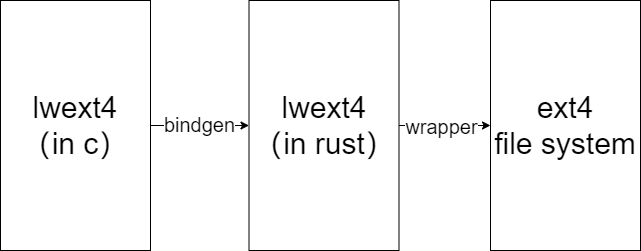
\includegraphics[width=0.6\linewidth]{figs/plan-ext.png}
    \caption{ext4 实现结构图}
    \label{ext4-complexe}
\end{figure}

\begin{enumerate}
    \item \textit{根据 lwext4 或者类似的库理清楚他的函数调用,必要的话给出一个 .h 文件用于包装函数入口:} \\ \textit{The wrapper.h file will include all the various headers containing declarations of structs and functions we would like bindings for. In the particular case of bzip2, this is pretty easy since the entire public API is contained in a single header. For a project like SpiderMonkey, where the public API is split across multiple header files and grouped by functionality, we'd want to include all those headers we want to bind to in this single wrapper.h entry point for bindgen.}\footnote{参考 bindgen 手册https://rust-lang.github.io/rust-bindgen/tutorial-2.html},这意味着,\textbf{对于一个比较复杂而分散的项目,我们最好给出一个包装文件}.
    \item \textit{对于转换完成的rs库,视情况给出rust调用}
    \item \textit{转换我们的fs适配新的rs库} \\ 这部分很简单,我们相当于已经拿来一个ext文件系统了,剩下的就是直接使用调用就行了。在makefile里和rust代码里加入feature就可以做到针对不同文件系统的编译与运行
\end{enumerate}

\vspace{1em}

对于其中可能出现的问题,可见如下列表:

\begin{enumerate}
    \item \textbf{移植的时候会不会出现不适配龙芯情况:}99\%不会,目前查出来 Bindgen 使用 Clang 对 C 文件进行编译,之后反编译(\textit{仅使用 Clang ,不使用 LLVM 编译为机器码})回 Rust ,所以生成的代码最后编译时间还是走的 make 中的 loongarch-gcc .具体编译环节的参考如下:https://blog.csdn.net/xhhjin/article/details/81164076
    \item \textbf{lwext4 的水平如何,是否会存在包本身的问题:} C 语言库,方便阅读;稳定性比较强,多平台测试过,支持小端序,测试过的架构有 x86/AMD64 , ARM 系列以及其的各种嵌入式架构
\end{enumerate}

\subsubsection{第一次适配(LWEXT4-C + Bindgen)}

在第一次适配中,我们试图通过上述方式完成 EXT4 文件系统对于 LA 的适配,然而,我们遇到了许多问题
\begin{enumerate} 
    \item \textit{no_std 环境问题:}我们发现,离开了标准 C 环境的 lwext4 的适配情况并没有我们想象的顺利。在一步步 debug 的过程中,我们经历了如下问题:
    \begin{figure}[htbp] 
        \centering 
        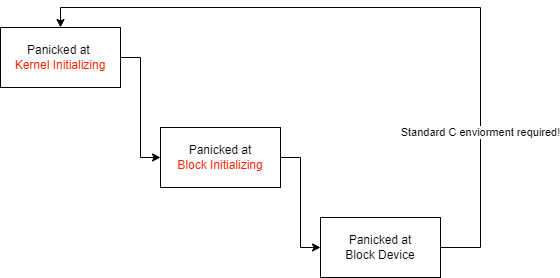
\includegraphics[width=0.5\linewidth]{figs/ext4c.png} 
        \caption{Debug 流程图} 
        \label{debug-ext4c} 
    \end{figure} 
\end{enumerate}

\subsubsection{第二次适配(LWEXT4-RUST)}

经过一定时间的查找资料,我们发现了下一个 lwext4 库,其 Supported Features 具体如下:\footnote{github网址:https://github.com/elliott10/lwext4_rust},然而这个包的适配过程仍然十分艰难:

\begin{itemize}
    \item lwext4_rust for x86_64, riscv64 and aarch64 on Rust OS is supported
    \item File system mount and unmount operations
    \item Filetypes: regular, directories, softlinks
    \item Journal recovery \& transactions
    \item memory as Block Cache
\end{itemize}

由于在其 Dependences 中发现了如下信息:

\begin{center}
    \textbf{C musl-based cross compile toolchains}
    \begin{itemize}
        \centering
        \item x86_64-linux-musl-gcc
        \item riscv64-linux-musl-gcc
        \item aarch64-linux-musl-gcc
    \end{itemize}
\end{center}

\textit{我们认为,其在我们拥有 LA 相关工具链的情况下是可以适配至我们的 LA 指令集操作系统上的}

经过一段时间的分析,我们认为 lwext4 系列的库\textbf{由于一定原因与 LA 指令集并不适配}

\subsubsection{第三次适配(EXT4-View)}

由于前两次适配都设计到lwext4相关,并且其存在于mkfs不相干的特性(但这并不是使用lwext4-mkfs没有成功的根本原因)。于是我们在github上自行检索并找到了这个EXT4-View\footnote{https://github.com/nicholasbishop/ext4-view-rs}仓库。我们试图将这个版本的EXT4与我们的NPUcore进行适配。

EXT4-View由一个谷歌研究员开发并持续维护中。该库提供了一个 Rust crate,允许对 ext4 文件系统进行\textbf{只读访问}。该 crate是no_std,因此可在嵌入式上下文中使用。不过,它需要 alloc。
这个仓库的基本属性可以总结为如下的部分:
\begin{enumerate}
    \item 所有有效的 ext4 文件系统都应该是可读的。
    \item 无效数据绝不会导致崩溃、panic或无限循环。
    \item 主软件包中没有不安全代码(允许在依赖包中出现)。
\end{enumerate}
使用方法为:
\begin{lstlisting}[language={Rust}, caption={ext4-view在kernel中的基本使用方法示例}]
use ext4_view::{Ext4, Metadata};

let fs_data: Vec<u8> = get_fs_data_from_somewhere();
let fs = Ext4::load(Box::new(data_source))?;

// If the std feature is enabled, you can load a filesystem by path:
let fs = Ext4::load_from_path(std::path::Path::new("some-fs.bin"))?;

// The Ext4 type has methods very similar to std::fs:
let path = "/some/file/path";
let file_data: Vec<u8> = fs.read(path)?;
let file_str: String = fs.read_to_string(path)?;
let exists: bool = fs.exists(path)?;
let metadata: Metadata = fs.metadata(path)?;
for entry in fs.read_dir("/some/dir")? {
    let entry = entry?;
    println!("{}", entry.path().display());
}
    \end{lstlisting}

而载入这个文件系统的方法只有两步,首先需要将img转换为.bin文件,并将.bin引入到kernel中,用一个指针指向它作为基本目录。实现代码如下:
\begin{lstlisting}[language={Rust}, caption={将测例加载进入kernel}]
    fn load_test_disk1() -> Ext4 {
        const DATA: &[u8] = include_bytes!("../../test_data/test_disk1.bin");
        Ext4::load(Box::new(DATA.to_vec())).unwrap()
    }

\end{lstlisting}

在适配中我们发现了两个明显的缺点:第一,由于加载kernel的地址为0x9000000090000000,计算后发现,只有64M的空间。所以我们的uImage大小不能超过64M,而本次全部测例有120M左右,因此没有办法将全部测例封装并测试。
第二,也是最致命的缺点。经过三天的适配后,我们发现内核中存在了很多奇怪的bug,包括但不限于找不到根目录,块设备加载出错等。刚开始我们认为是我们的kernel适配没有完全成功,而经过检查后发现是仓库本身存在问题,目前的版本不是完全完善的ext4版本。
而该仓库也仅有一个只读文件系统,没有办法完成针对本次比赛“完整的”EXT4适配,因此我们最终也放弃了这个仓库。

这个仓库值得后续的高度关注,因为它代码风格统一,接口完善,适配简单,应该能成为后续适配者的一个优质选择。

\subsubsection{第四次适配(Alien-rust)}

最后抱着试一试的态度,我们找到了往年的特等奖得主Alien\footnote{https://gitlab.eduxiji.net/202310007101563/Alien}仓库(该仓库仍然在持续开源并推进中。它一个用 rust 实现的简单操作系统。目的是探索如何使用模块来构建一个完整的操作系统,因此系统由一系列独立的模块组成。

他们的仓库中有提到对于lwext4的修复与推进工作:有了c实现的支持,我们只需要在rust中生成相关的头文件以及静态库。在做这部分之前,我们首先查看了一下crates.io中是否已有相关的实现,幸运的是,2年前已经有一个实现lwext4, 在简单阅读了其实现之后,我们打算参考其实现重新编写,因为其已经缺乏维护,并且不包含对no_std环境的支持。这个已有的实现给予我们很好的想法。
最终我们根据Alien的提示,适配了一个仍然针对LA2K1000开发板存在bug的NPUcore版本。该版本仅支持执行部分测例,并没有实现完整的“文件系统”应有的部分。但是我们仍将我们针对这个仓库的适配过程做一个小总结。

首先我们需要将文件系统从原先的FAT32转换为lwext4中的对应的Inode和FileSystem。这里的EasyFileSystem是一层针对文件系统的抽象接口。
\begin{lstlisting}[language={Rust}, caption={FILE_SYSTEM修改}]
pub type EasyFileSystem = lwext4_rs::FileSystem<crate::arch::BlockDeviceImpl>;
type DiskInodeType = lwext4_rs::FileType;
    lazy_static! {
        pub static ref FILE_SYSTEM: EasyFileSystem = EasyFileSystem::new(
            MountHandle::mount(
                RegisterHandle::register(BlockDevice::new(BlockDeviceImpl::new()), "shit".to_string())
                    .unwrap(),
                "/".to_string(),
                false,
                false,
            )
            .unwrap()
        )
        .unwrap();
    }
\end{lstlisting}

我们针对这层抽象继续修改对应的根目录:
\begin{lstlisting}[language={Rust}, caption={ROOT修改}]
    lazy_static! {
        pub static ref ROOT: Arc<DirectoryTreeNode> = {
            FILE_SYSTEM.readdir("/").unwrap();
    
            let inode = DirectoryTreeNode::new(
                "".to_string(),
                Arc::new(FileSystem::new(FS::Fat32)),
                Arc::new(OpenOptions::new().read(true).write(true).open("/").unwrap()),
                // OSInode::new(Arc::new()),
                Weak::new(),
            );
            inode.add_special_use();
            inode
        };
        static ref DIRECTORY_VEC: Mutex<(Vec<Weak<DirectoryTreeNode>>, usize)> =
            Mutex::new((Vec::new(), 0));
        static ref PATH_CACHE: Mutex<(String, Weak<DirectoryTreeNode>)> =
            Mutex::new(("".to_string(), Weak::new()));
    }
    \end{lstlisting}

针对这层块设备,我们也适配了对应的PCI和SATA块的读写部分,可以识别到测例。这里的lock和unlock方法为开发中,因为诸多测例都不需要这个方法,close则为默认关闭成功。
\begin{lstlisting}[language={Rust}, caption={ROOT修改}]
    impl lwext4_rs::BlockDeviceInterface for SataBlock{
        fn read_block(&mut self, buf: &mut [u8], mut block_id: u64, block_count: u32) -> lwext4_rs::Result<usize> {
            // kernel BLOCK_SZ=2048, SATA BLOCK_SIZE=512,four times
            block_id = block_id * (BLOCK_SZ as u64 / BLOCK_SIZE as u64);
            for buf in buf.chunks_mut(BLOCK_SIZE) {
                self.0
                    .lock()
                    .read_block(block_id, buf);
                block_id += 1;
            }
            Ok(0)
        }
    
        fn write_block(&mut self, buf: &[u8], mut block_id: u64, block_count: u32) -> lwext4_rs::Result<usize> {
            block_id = block_id * (BLOCK_SZ as u64 / BLOCK_SIZE as u64);
            for buf in buf.chunks(BLOCK_SIZE) {
                self.0
                    .lock()
                    .write_block(block_id, buf);
                block_id += 1;
            }
            Ok(0)
        }
        
        fn close(&mut self) -> lwext4_rs::Result<()> {
            Ok(())
        }
    
        fn open(&mut self) -> lwext4_rs::Result<lwext4_rs::BlockDeviceConfig> {
            Ok(lwext4_rs::BlockDeviceConfig{
                block_size: BLOCK_SIZE as u32,
                block_count: 999,
                part_size: BLOCK_SIZE as u64 * 2,
                part_offset: 0
            })
        }
    
        fn lock(&mut self) -> lwext4_rs::Result<()> {
            Ok(())
        }
    
        fn unlock(&mut self) -> lwext4_rs::Result<()> {
            Ok(())
        }
    }
    \end{lstlisting}
    
我们最终在决赛提交的也是这个版本,虽然它仍然有各种问题,但是我们将测例直接放入kernel中是可以跑出对应分数的。这个文件系统适配仍然非常不完善,甚至在文件系统初始化时都会报panic(我们跳过文件系统这一层,直接执行测例跑出的分数),因此我们后续仍然会持续推进并开发。
\section{用户地址空间}
\begin{figure}[htb]
    \centering
    \includegraphics[width=\textwidth]{figures/figure1.pdf}
    \caption{
        用户虚拟地址空间示意
    }
    \label{fig:user virtual process}
\end{figure}
每一个进程都有一个独立的页表,当npucore实现进程切换的时候,对应的页表也会切换。

当一个用户进程通过系统调用向操作系统请求更多的用户空间时,npucore首先在os/src/frame_allocator.rs中的StackFrameAllocator的基于栈的数据结构实现空闲物理页的分配,然后将物理页的映射加入到用户的页表当中。
npucore将设置PTEflags::R,PTEflags::W,PTEflags::U,PTEflags::X以及PTEflags::V标志位到对应的页表项目,使得用户可以对分配的页面进行读写操作。
大多数的用户进程并不能完全利用所有的虚拟空间,对于没有用到的空间,它对应的页表项PTEflags::V标志位始终为0。

页表的设计有很多的好处。首先,首先不同的进程使用不同的页表,相同的虚拟地址映射到不同的物理地址,因此每一个进程可以拥有自己独立的内存空间。其次,用户的虚拟地址是连续的,对应的物理地址不一定是连续的,这样可以有效的避免内存碎片。最后,内核将所有的用户的跳板代码都映射到了同一段虚地址,可以有效的实现上下文切换。

如图\ref{fig:user virtual process}所示,用户的虚拟地址空间被分为了三个部分,分别是用户代码段,用户数据段以及用户堆栈段。用户代码段用于存放用户的代码,用户数据段用于存放用户的数据,用户堆栈段用于存放用户的堆栈。
其中,用户栈的初始内容如图中所示,由execve函数完成初始化,其中包含了用户的命令行参数和返回地址,紧接着就是main函数使用的栈空间。

npucore实现了execve来将elf文件加载到内存的进程地址空间中,实现了sbrk来动态的分配用户空间,实现了mmap来将文件映射到用户空间,实现了munmap来取消文件的映射。

\subsection{sbrk系统调用}
sbrk系统调用是早期的Unix系统中的一个系统调用,用于动态的分配用户空间。sbrk系统调用的原型如下:
\begin{lstlisting}[language=c]
    void *sbrk(intptr_t increment);
\end{lstlisting}
sbrk系统调用将堆的大小增加increment字节,并返回堆的起始地址。
如果increment为负数,则堆的大小减少increment字节。如果堆的大小超过了进程的地址空间,则sbrk系统调用返回-1,并设置errno为ENOMEM。
sbrk系统调用可以为一个进程扩大或者缩小堆的大小,主要的实现是由os/src/memory_set.rs中的sbrk函数完成。
sbrk函数调用Memoryset::mmap或者Memoryset::munmap来实现堆的扩大或者缩小。
mmap函数不仅用于sbrk系统调用,还用于mmap系统调用,用于将文件映射到用户空间和开辟匿名内存映射。
\begin{lstlisting}[language=rust]
    pub fn sbrk(&mut self, heap_pt: usize, heap_bottom: usize, increment: isize) -> usize {
        let old_pt: usize = heap_pt;
        let new_pt: usize = old_pt + increment as usize;
        // 判断扩大堆还是缩小堆
        if increment > 0 {
            let limit = heap_bottom + USER_HEAP_SIZE;
            if new_pt > limit {
                return old_pt;
            } else {
                self.mmap(
                    old_pt,
                    increment as usize,
                    MapPermission::R | MapPermission::W | MapPermission::U,
                    MapFlags::MAP_ANONYMOUS | MapFlags::MAP_FIXED | MapFlags::MAP_PRIVATE,
                    1usize.wrapping_neg(),
                    0,
                );
                trace!("[sbrk] heap area expanded to {:X}", new_pt);
            }
        } else if increment < 0 {
            // 如果缩小后的堆地址小于堆底地址,则不进行缩小
            if new_pt <= heap_bottom {
                return old_pt;
            } else {
                self.munmap(old_pt, increment as usize).unwrap();
            }
        }
        new_pt
    }
\end{lstlisting}

\chapter{进程管理}
\section{进程生命周期和资源复用}
\subsection{进程生命周期}
进程指的是在系统中运行的一个程序的实例。而进程的生命周期包括从创建,阻塞,唤醒,退出等。
为了可以在npucore上同时运行多个进程,npucore实现了进程的创建,在内核中加载进程到内存,同时为其分配系统资源。
npucore为每一个进程分配系统资源,包括内存、文件描述符、CPU等,而实现系统资源的分配的方式是通过系统调用fork。
npucore中,fork系统调用用于创建一个新的进程,新的进程称为子进程,原来的进程称为父进程。
而所有的其他进程都是initproc的子进程,他们通过fork得到。initproc是需要在内核启动过程中创建的第一个进程。
对应的代码如下:
\begin{lstlisting}[language=rust]
    lazy_static! {
    pub static ref INITPROC: Arc<TaskControlBlock> = Arc::new({
        let elf = ROOT_FD.open("initproc", OpenFlags::O_RDONLY, true).unwrap();
        TaskControlBlock::new(elf)
    });
}
\end{lstlisting}
当创建一个新的进程时,用户进程通过fork得到一个原本进程的副本,为其分配系统资源,然后调用execve来讲elf文件加载到内存以创建一个新的进程。
每个进程都有自己的内存空间、代码和数据,它们是系统中资源的分配单位。他们的创建是由elf文件指定的。

为了保证所有的进程都能够被调度,从而避免进程饥饿的发生,npucore实现了进程的调度机制,从而实现阻塞和唤醒。
当一个进程主动放弃CPU或者被动的被剥夺CPU的使用权时,它会让出CPU,变成等待状态,这个过程称为阻塞。
在进程的视角看来,他会有一个自己独占CPU的“幻觉”,因为每一个阻塞和唤醒的时候进程的状态总是保持不变的。这样可以保证进程执行的正确性。
而npucore让一个被阻塞的进程重新开始执行的行为叫做唤醒。唤醒的同时会恢复进程的现场,包括阻塞时的寄存器状态。

而当一个进程执行结束,它就会退出,将它所占有的系统资源释放。进程的退出保证了npucore避免出现资源的永久占用的情况。
上述过程就是一个进程从“生”到“死”,保证了npucore可以正确且高效的执行对应的程序。

\subsection{资源复用}
为了实现多进程同时运行,操作系统需要对CPU,内存,外设等资源进行复用。
复用在资源有限的情况下是一个常用且实际的思想。围绕着复用的思想,我们可以提出以下几个问题:

如何实现上下文切换?

虽然保存现场思想是简单的,但是实际的实现却不是那么显然。在npucore中我们使用了一段所有进程共享的跳板代码和一个进程的私有的保存现场的帧来实现。

如何让进程如何实现透明调度,也就是用户进程不知道自己被调度了?

npucore实现了内置的计时器,当计时器中断发生时,内核会调用schedule函数,从而实现进程的调度。

进程的资源回收不能由进程自己来完成,否则进程退出时会出现资源泄露的情况,如何实现进程的资源回收?

npucore在exit之后,会释放一部分资源,但是不会释放所有的资源,从而进入僵尸状态,父进程来完成剩下的进程资源的回收。

如何在并发的情况下不会错过对进程的唤醒?

npucore中是一个单核的操作系统,在进入关键代码的时候会保证CPU不会调度其他进程,从而保证了进程的唤醒不会被错过。
\section{进程状态控制}

\subsection{基本概念}

在操作系统课程的学习中我们知道 ,进程其实是一个“执行中的程序”。程序是一个没有生命的实体 ,只有 在操作系统执行静态的、放在磁盘中的代码段时 ,它才能成为一个活动的实体 ,我们称其为进程。

在运行过程中 ,进程是一个实体。每一个进程都有它自己的地址空间 ,一般情况下 ,包括文本区域  (text  region)  、数据区域  (data region)  和堆栈  (stack region)  。文本区域存储处理器执行的代码 ;数据区域 存储变量和进程执行期间使用的动态分配的内存 ;堆栈区域存储着活动过程调用的指令和本地变量。
\begin{figure}[H]
	\centering
	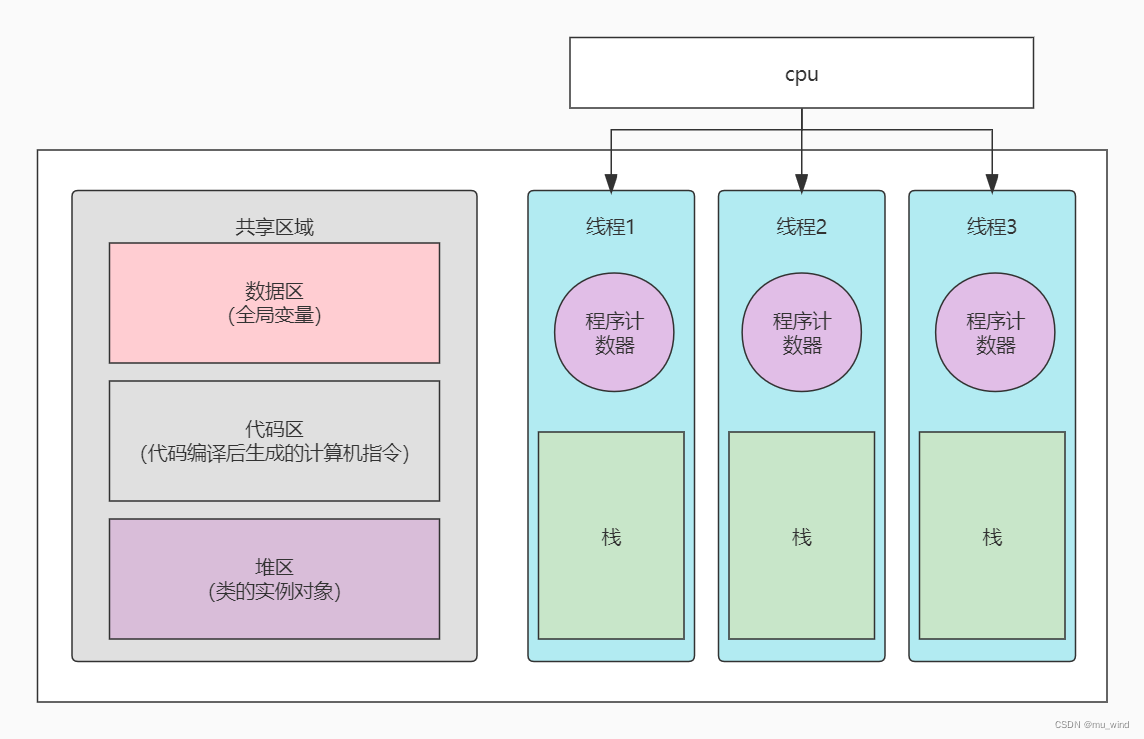
\includegraphics[width=14cm,height=8cm]{figures/04-02-01-进程的数据结构.png}
	\caption{进程的数据结构}
\end{figure}  

进程的创建、销毁与切换存在着较大的时空开销,一种轻型的进程技术线程用来减少开销。线程被设计成进程的一个执行路径,同一个进程中的线程共享进程的资源,因此系统对线程的调度所需的成本远远小于进程。

\begin{figure}[h]
	\centering
	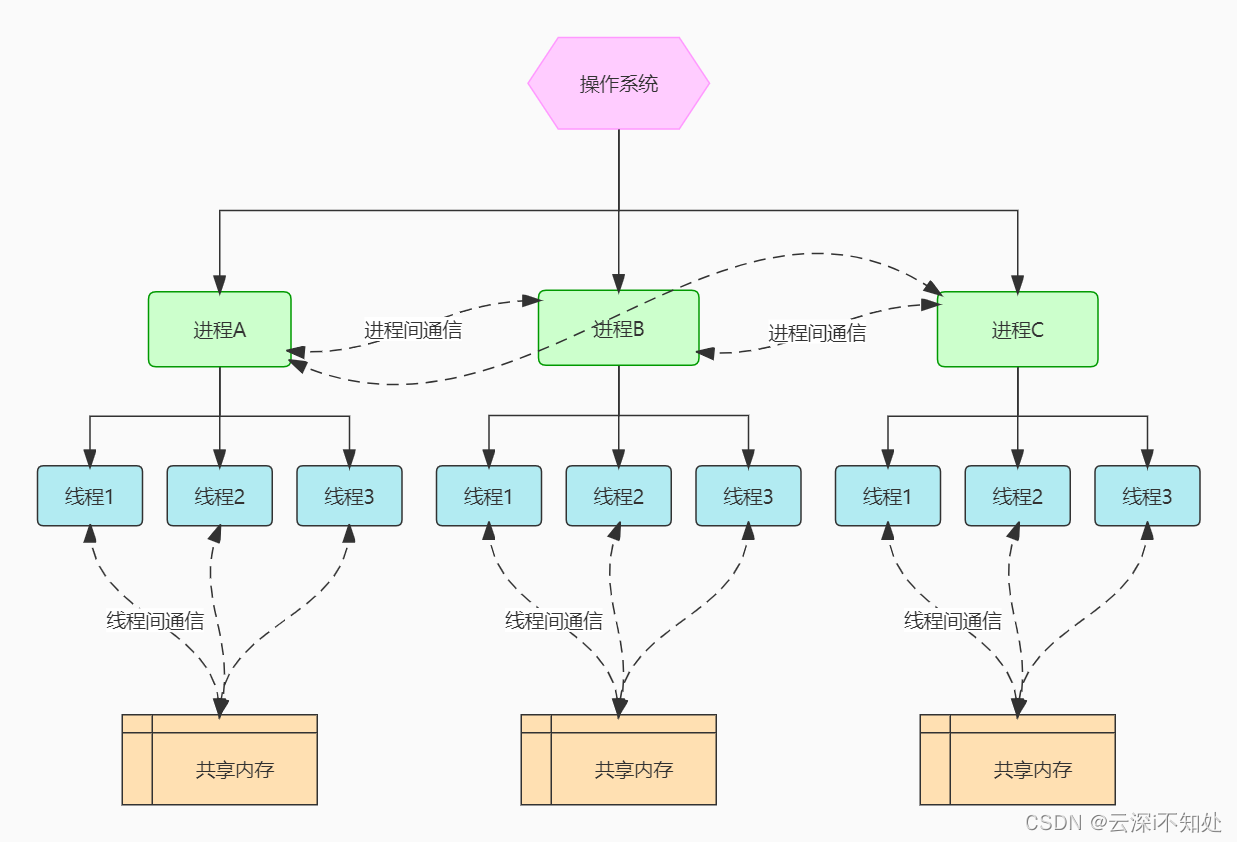
\includegraphics[width=14cm,height=11cm]{figures/04-02-01-线程与进程间的关系.png}
	\caption{线程与进程间的关系}
\end{figure}  

在 NPUcore 中 ,我们使用 TCB结构体来描述一个进程 ,该结构体可以完整地描述一个进程的内容和结构。 利用该结构体 ,我们可以像 linux 一样使用进程来模拟线程。这与windows操作系统的设计思路是不同的,其线程的实现依靠单独的一套 thread\_control\_block 完成。
 
因此线程在 NPUcore 中的理解变为了这样——一个可以与同线程组( tg1d 共享内存空间的进程即为线程。

NPUCore进程管理的代码树如下:
\begin{lstlisting}[language=R]
	os
	|--src
	|--task
	|--context.rs //存储上下文信息
	|--elf.rs //ELF文件加载和解析
	|--manager.rs //任务管理器的结构存储
	|--mod.rs//任务操作系统任务管理和调度的实现
	|--pid.rs//实现内核栈、进程分配器、内核栈分配器等数据结构及操作
	|--processor.rs // 进程轮询的主体和processor的声明与实现
	|--signal.rs //
	|--switch.rs //调用switch汇编函数的接口,实现任务上下文切换
	|--switch.S //任务上下文切换的汇编实现
	|--threads.rs//实现用户空间多线程快速互斥锁(Futex)
	|--task.rs //涉及TCB模块的声明以及方法的实现,以及rusage信号量的声明。
\end{lstlisting}

\subsection{进程管理重要数据结构}
\subsubsection{进程标识符\ PidHandle}
同一时间存在的所有进程都有一个唯一的进程标识符,将其抽象为 PidHandle 类型。
\begin{lstlisting}[language=R]
	//os/src/task/pid.rs
	pub struct PidHandle(pub usize);
\end{lstlisting}

进程标识符是一个64位的无符号整数 ,用来标识进程ID。进程标识符的分配和回收由标识符分配 器 RecycleAllocator 完成。我们一般简称其为 PID。

\subsubsection{内核栈\ KernelStack}
内核在创建进程的时候 ,在创建task\_struct的同时 ,会为进程创建两个栈 ,第一个栈也就是上面分析到的 进程用户栈 ,存在于用户空间使用 ,另外还有一个内核栈 ,存放在内核空间。

\textbf{内核栈存在的意义 :}如系统调用在陷入内核后 ,系统调用中也是存在函数调用和自动变量 ,这些都需 要栈支持。

\textbf{每个进程都要有独自的内核栈的必要性:}所有进程在运行时 ,都有可能通过系统调用陷入内核态继续 执行 ,假设第一个进程陷入内核执行的时候,需要等待某个资源,主动schedule() ,让出CPU ,第二个进 程假设也通过系统调用进入了内核态 ,如果进程共享内核栈 ,那么第二个进程在系统调用压栈时会破坏第一个进程栈数据。

每个应用都有自己的内核栈 ,因此 KernelStack 的内部就是其所属进程的 PID 号。

\begin{lstlisting}[language=R]
	//os/src/task/pid.rs
	pub struct KernelStack(pub usize);
\end{lstlisting}

它提供了以下方法 :

1.返回当前内核栈在内核空间中的栈顶和栈底位置 :
\begin{lstlisting}[language=R]
	pub fn kernel_stack_position(kstack_id : usize) -> (usize, usize) {
		let top = TRAMPOLINE - kstack_id * (KERNEL_STACK_SIZE + PAGE_SIZE);
		let bottom = top - KERNEL_STACK_SIZE;
		(bottom, top)
	}
\end{lstlisting}

2.内核栈分配器 :
\begin{lstlisting}[language=R]
	pub fn kstack_alloc() -> KernelStack {
		let kstack_id = KSTACK_ALLOCATOR .lock() .alloc();
		let (kstack_bottom, kstack_top) = kernel_stack_position(kstack_id);
		KERNEL_SPACE .lock() .insert_framed_area(
		kstack_bottom .into(),
		kstack_top .into(),
		MapPermission : :R | MapPermission : :W,
		);
		KernelStack(kstack_id)
	}
\end{lstlisting}

该分配器先从全局实例化的 KSTACK\_ALLOCATOR 中获取内核栈编号。  它调用了  kernel\_stack\_position
函数来根据进程标识符计算内核栈在内核地址空间中的位置 ,随即将一个逻辑段插入内核地址空间 KERNEL\_SPACE 中  (详情见内存管理章节)。

3.将内核栈从内核空间中移除 :
\begin{lstlisting}[language=R]
	impl Drop for KernelStack {
		fn drop(&mut self) {
			let (kernel_stack_bottom, _) = kernel_stack_position(self .0);
			let kernel_stack_bottom_va : VirtAddr = kernel_stack_bottom .into();
			KERNEL_SPACE
			.lock()
			.remove_area_with_start_vpn(kernel_stack_bottom_va .into())
			.unwrap();
			KSTACK_ALLOCATOR .lock() .dealloc(self .0)
		}
	}
\end{lstlisting}

4.push\_on\_top 方法 :
\begin{lstlisting}[language=R]
	impl KernelStack {
		#[allow(unused)]
		pub fn push_on_top<T>(&self, value : T) -> *mut T
		where
		T : Sized,
		{
			let kernel_stack_top = self .get_top();
			let ptr_mut = (kernel_stack_top - core : :mem : :size_of : :<T>()) as *mut T;
			unsafe {
				*ptr_mut = value;
			}
			ptr_mut
		}
		pub fn get_top(&self) -> usize {
			let (_, kernel_stack_top) = kernel_stack_position(self .0);
			kernel_stack_top
		}
	}
\end{lstlisting}

该方法可以将一个类型为  T 的变量压入内核栈顶并返回其裸指针 ,这也是一个泛型函数。  它在实现的时 候用到了  get\_top 方法来获取当前内核栈顶在内核地址空间中的地址。

\subsubsection{进程控制块}
为了使并发执行的程序独立运行 ,描述进程的基本情况和活动过程 ,进而管理和控制进程 ,操作系统专门 配置了⼀个数据结构——进程控制块。在 NPUcore 中 ,我们使用 TCB 这一名字代替 PCB 来同时用作进程控制块和线程控制块。但是在本章中 ,为了简化逻辑 ,我们尽量只讨论单线程的情况 ,也就是仅仅 把 TCB 看作是进程控制块。

TCB作为进程实体的一部分 ,记录了操作系统所需的 ,描述进程的当前情况以及管理进程运行的全部信 息 ,是操作系统中最重要的数据结构。整个进程管理模块,正是围绕着TCB数据结构的生命周期来展开,通过控制TCB模块的生命周期来实现进程的创建,调度和回收。

1.作为独立运行基本单位的标志 :当一个程序  (含数据)  配置了TCB后 ,就标志着它已经是一个能在多道程序环境下独立运行、合法的基本单位。系统是通过TCB感知进程的存在的 ,TCB已成为进程存在 于系统 的唯一标志。

2.能实现间断性运行方式 :当进程因阻塞而暂停运行时 ,他必须保留运行时的CPU现场信息 ,再次被调
度运行时 ,还需要恢复运行时的CPU现场信息。在有了TCB后 ,系统将CPU现场信息保存在被中断进 程的TCB中 ,供该进程再次被调度时恢复其CPU现场信息 。  由此可知 ,在多道程序环境下 ,传统意义 上的程序无法保护自身运行环境 ,无法保证其执行结果的可再现性 ,失去运行意义。

3.提供进程管理所需的信息 :当调度某进程运行时 ,只能根据该进程TCB只能记录的程序和数据的始址
指针 ,来找到相应的程序和数据 ;在进程运行期间 ,  当需要访问文件系统中的文件或I/O设备时 ,也需 要借助TCB中的信息。可见 ,在进程的生命周期中 ,操作系统总是根据TCB中的信息来控制和管理进 程。

4.提供进程调度所需的信息 :只有处于就绪状态的进程才能被调度执行 ,而TCB就提供了该进程处于何
种状态的信息。H

5.实现与其他进程的同步和通信

在NPUcore中 ,任务控制块 TCB(Task Control Block) 将直接作为 PCB 进行使用。下图是NPUcore中进 程控制块的具体组成。

\begin{figure}[H]
	\centering
	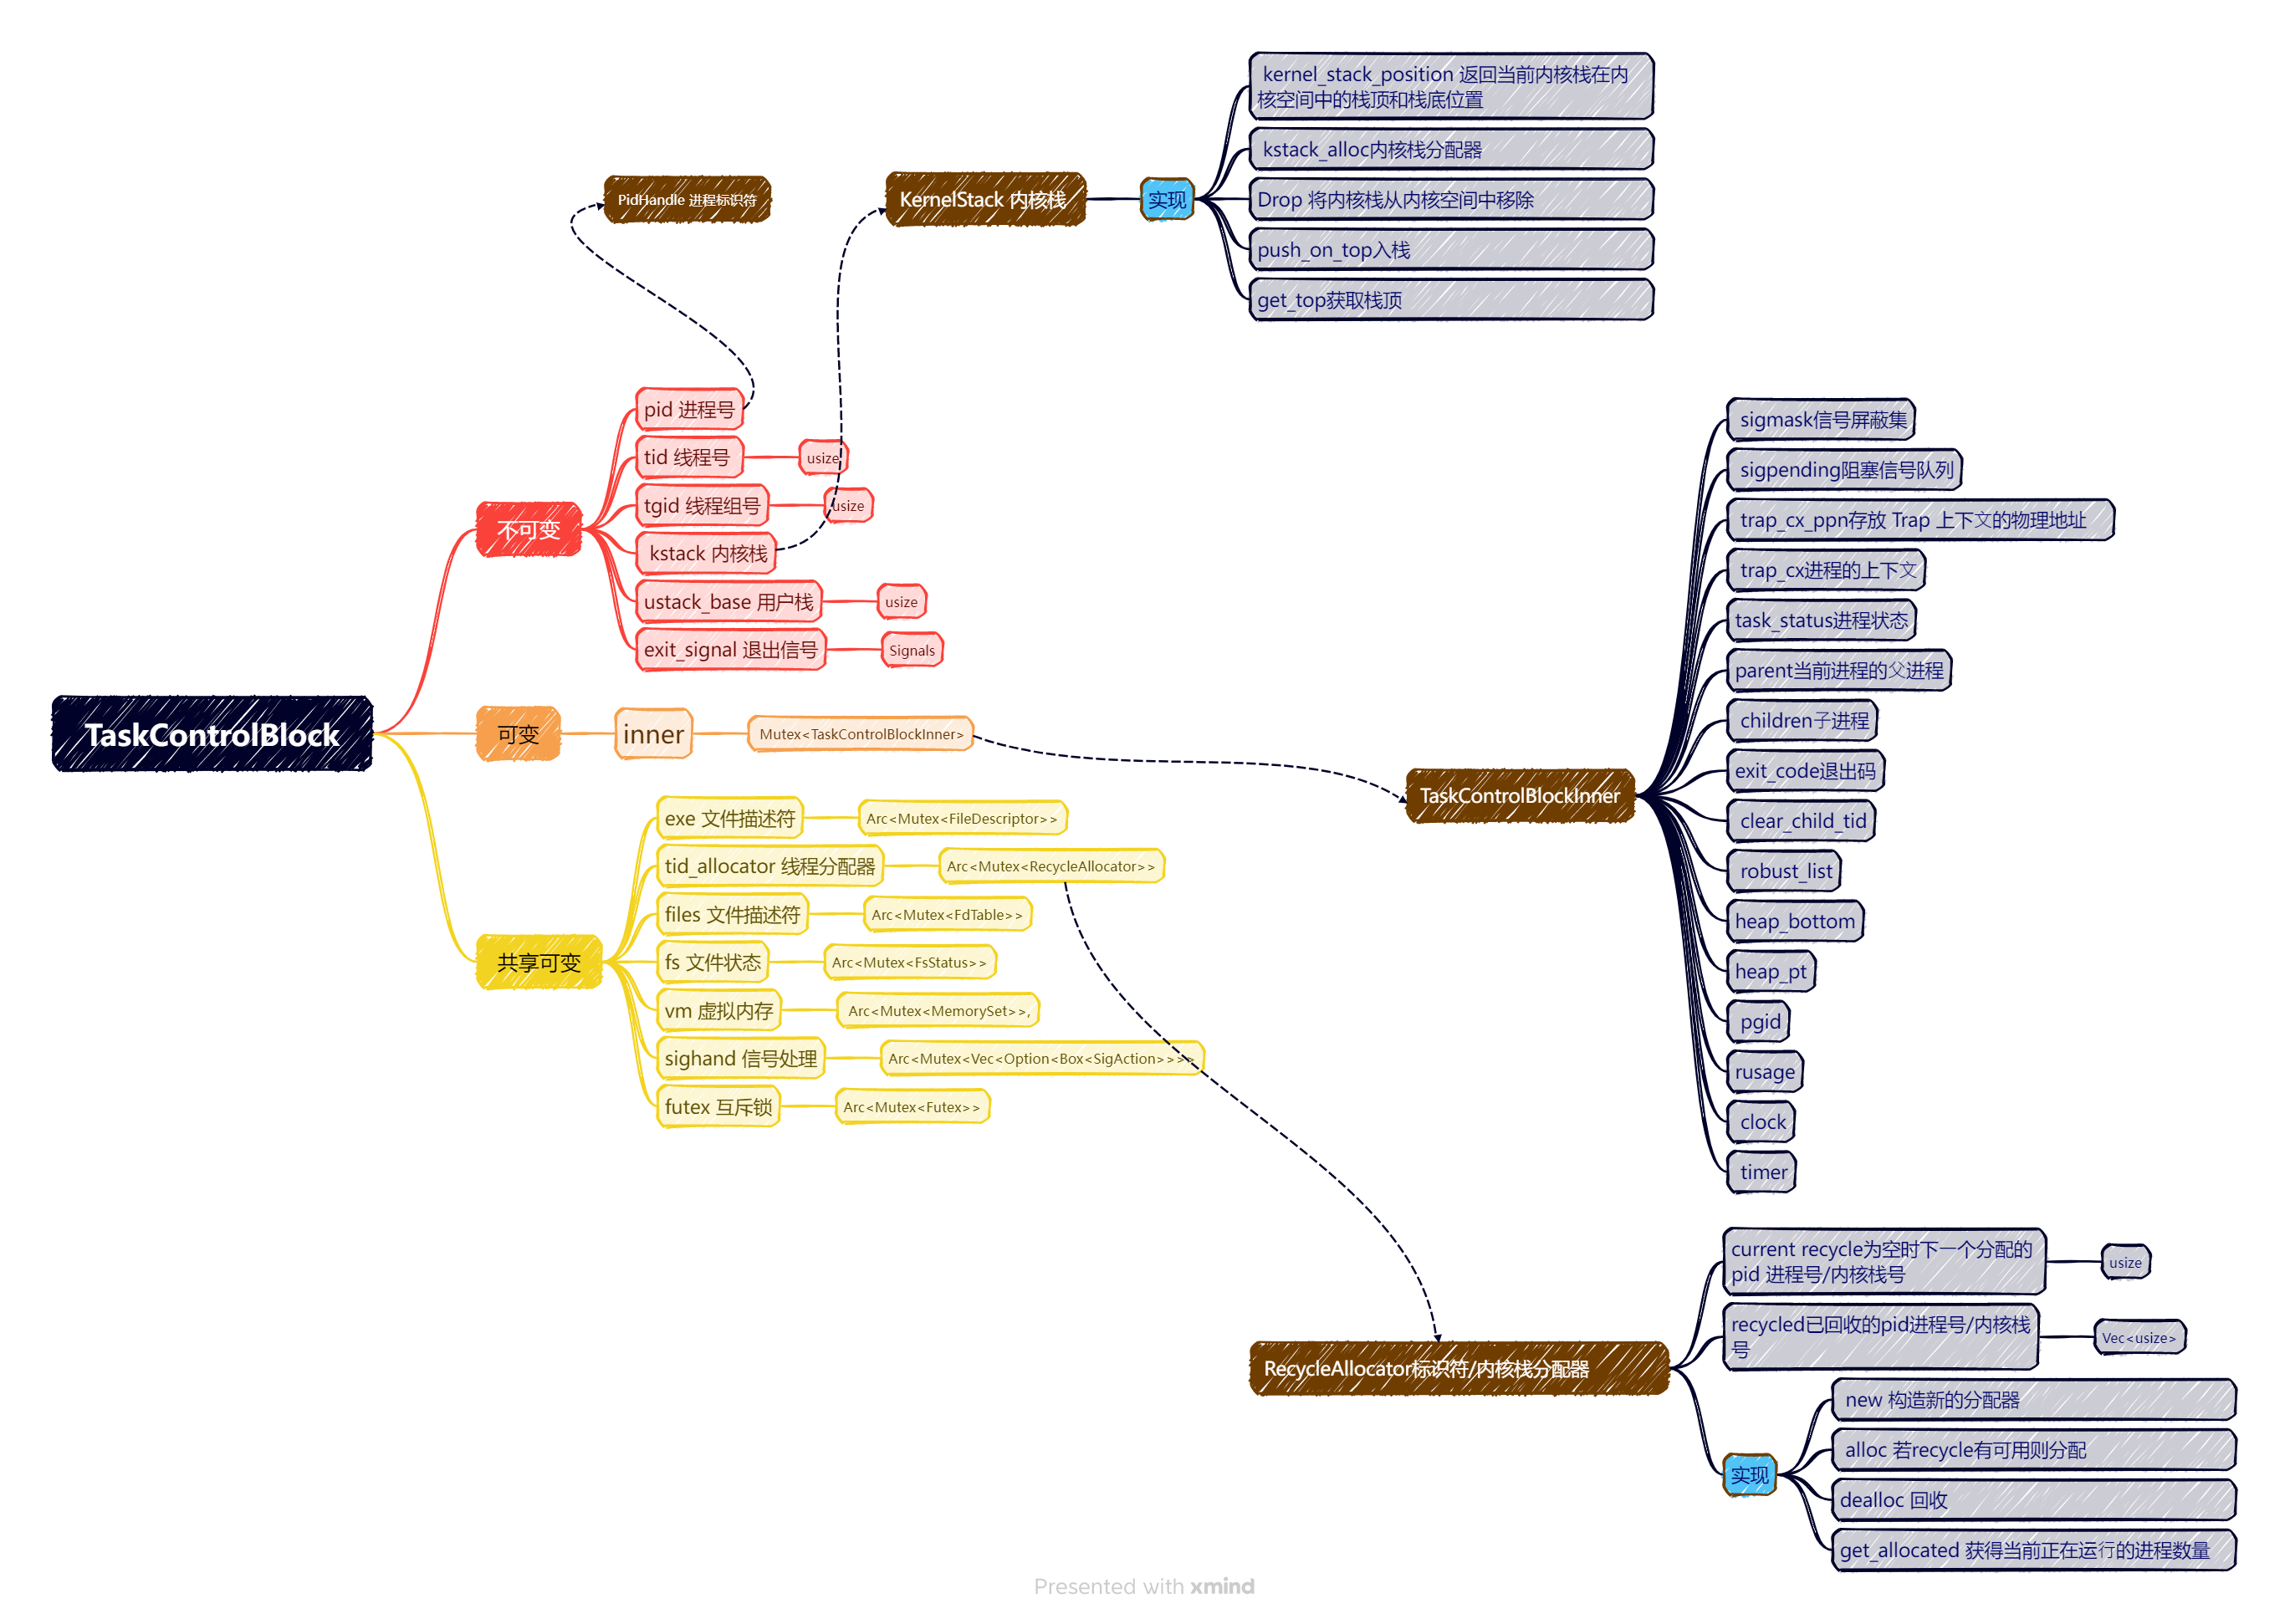
\includegraphics[width=14cm,height=11cm]{figures/04-02-01-NPUcore中进程控制块的具体组成.png}
	\caption{NPUcore中进程控制块的具体组成}
\end{figure}    

由于该数据结构的成员过多 ,且很多成员变量都是与信号及多线程的锁相关的 ,因此这里只挑选部分成员 变量进行讲解。

\begin{lstlisting}[language=R]
	//os/src/task/task.rs
	pub struct TaskControlBlock {
		// immutable
		pub pid : PidHandle,
		pub tid : usize,
		pub tgid : usize,
		pub kstack : KernelStack,
		pub ustack_base : usize,
		pub exit_signal : Signals,
		// mutable
		inner : Mutex<TaskControlBlockInner>,
		// shareable and mutable
		pub exe : Arc<Mutex<FileDescriptor>>,
		pub tid_allocator : Arc<Mutex<RecycleAllocator>>,
		pub files : Arc<Mutex<FdTable>>,
		pub fs : Arc<Mutex<FsStatus>>,
		pub vm : Arc<Mutex<MemorySet>>,
		pub sighand : Arc<Mutex<Vec<Option<Box<SigAction>>>>>,
		pub futex : Arc<Mutex<Futex>>,
	}
	pub struct TaskControlBlockInner {
		pub sigmask : Signals,
		pub sigpending : Signals,
		pub trap_cx_ppn : PhysPageNum,
		pub task_cx : TaskContext,
		pub task_status : TaskStatus,
		pub parent : Option<Weak<TaskControlBlock>>,
		pub children : Vec<Arc<TaskControlBlock>>,
		pub exit_code : u32,
		pub clear_child_tid : usize,
		pub robust_list : RobustList,
		pub heap_bottom : usize,
		pub heap_pt : usize,
		pub pgid : usize,
		pub rusage : Rusage,
		pub clock : ProcClock,
		pub timer : [ITimerVal; 3],
	}
\end{lstlisting}

TCB 由可变部分、不可变部分及可共享且可变部分组成。

1.不可变部分 :

( 1)   pid :进程号在进程创建后就是唯一的身份标识 ,所以肯定不变。  它的类型是 PidHandle 	

(2)   kstack :这是每个应用的内核栈。

(3)  ustack base: 用户栈的基地址 

(4)  exit signal: 退出信号

2.可变部分:inner : Mutex<TaskControlBlockInner>

TaskControlBlockInner 结构体的定义如下 :

\begin{lstlisting}[language=R]
	pub struct TaskControlBlockInner {
		pub sigmask : Signals,
		pub sigpending : Signals,
		pub trap_cx_ppn : PhysPageNum,
		pub task_cx : TaskContext,
		pub task_status : TaskStatus,
		pub parent : Option<Weak<TaskControlBlock>>,
		pub children : Vec<Arc<TaskControlBlock>>,
		pub exit_code : u32,
		pub clear_child_tid : usize,
		pub robust_list : RobustList,
		pub heap_bottom : usize,
		pub heap_pt : usize,
		pub pgid : usize,
		pub rusage : Rusage,
		pub clock : ProcClock,
		pub timer : [ITimerVal; 3],
	}
\end{lstlisting}	

同上 ,我们也不介绍信号与锁相关的成员变量。

trap\_cx\_ppn :这个东西的作用是把存放 Trap 上下文的物理地址拿出来 ,从而便于使用

\begin{lstlisting}[language=R]
	let trap_cx_ppn = memory_set
	.translate(VirtAddr : :from(TRAP_CONTEXT) .into())
	.unwrap()
	.ppn();
	
	task_cx :类型是 TaskContext ,是进程的上下文
	
	pub struct TaskContext {
		/// return address ( e .g . __restore ) of __switch ASM function
		ra : usize,
		/// kernel stack pointer of app
		sp : usize,
		/// s0-11 register, callee saved
		s : [usize; 12],
	}
\end{lstlisting}

TaskManager:进程管理模块,维护两个循环队列,一个是就绪态队列,一个是阻塞态任务队列,队列中的内容都是TCB模块的指针。
\begin{lstlisting}[language=R]
	pub struct TaskManager {
		pub ready_queue:
		VecDeque<Arc<TaskControlBlock>>,
		pub interruptible_queue:
		VecDeque<Arc<TaskControlBlock>>,
	}
\end{lstlisting}
ready\_queue:就绪态队列

interruptible\_queue:阻塞态任务队列

Processor:用于保存当前任务的arc指针和空闲的任务上下文(用于进程切换)。
\begin{lstlisting}[language=R]
	pub struct Processor {
	current: Option<Arc<TaskControlBlock>>,
	idle_task_cx: TaskContext,
}
\end{lstlisting}
current 表示在当前处理器上正在执行的任务
\
idle\_task\_cx 表示当前处理器上的 idle 控制流的任务上下文

TaskStatus:基本的任务状态枚举,包括就绪态,运行态,僵尸态(等待回
收),阻塞态(等待激活以进入就绪态)。
\begin{lstlisting}[language=R]
	pub enum TaskStatus {
	Ready,
	Running,
	Zombie,
	Interruptible,
}
\end{lstlisting}

说明进程有四种状态 :就绪 、正在运行、“僵尸”状态  (表示该进程即将被回收)  以及可中断状态。

parent 是 TCB 的一个弱引用 ,他表示当前进程的父进程 ,同理 children 表示子进程exit\_code , 当进程调用  exit 系统调用主动退出或者执行出错由内核终止的时候 ,它的退出码exit\_code 会被内核保存在它的任务控制块中 ,并等待它的父进程通过  waitpid 回收它的资源的同时也 收集它的 PID 以及退出码。

\subsubsection{标识符/内核分配器\ RecycleAllocator}
对于进程标识符和内核栈,NPUCore都使用 RecycleAllocator 分配器来分配和回收。
\begin{lstlisting}[language=R]
	//os/src/task/pid.rs
	pub struct RecycleAllocator {
		current : usize,
		recycled : Vec<usize>,
	}
\end{lstlisting}

current 为若 recycled 数组为空时下⼀个分配的 pid 进程号/内核栈号 ,每次分配后都会+1 ; recycled 数组保存了当前已回收的 pid 进程号/内核栈号。

该分配器实现了以下四个方法 :

\begin{lstlisting}[language=R]
	impl RecycleAllocator {
		pub fn new() -> Self {
			RecycleAllocator {
				current : 0,
				recycled : Vec : :new(),
			}
		}
		pub fn alloc(&mut self) -> usize {
			if let Some(id) = self .recycled .pop() {
				id
			} else {
				self .current += 1;
				self .current - 1
			}
		}
		pub fn dealloc(&mut self, id : usize) {
			assert !(id < self .current);
			assert !(
			!self .recycled .iter() .any( |i| *i == id),
			"id {} has been deallocated !",
			id
			);
			self .recycled .push(id);
		}
		pub fn get_allocated(&self) -> usize {
			self .current - self .recycled .len()
		}
	\end{lstlisting}
	
	new() :构造方法 。只会在第⼀次实例化时调用。
	
	alloc(\&mut self) :分配器。若 recycled 数组中有可使用的 pid 号/内核栈号 ,则直接分配 ,否则 生成⼀个新的 pid 号。
	
	dealloc(\&mut self, id: usize):回收器。需要检查合法性才会回收。
	
	get\_allocated(\&self) :获得当前正在运行的进程数量。
	
	有了分配器后 ,我们可以将进程分配器分别实例化,
	
	实例化进程标识符分配器和内核栈分配器:
	\begin{lstlisting}[language=R]
		lazy_static ! {
			static ref PID_ALLOCATOR : Mutex<RecycleAllocator> = Mutex : :new(RecycleAllocator : :new()
			static ref KSTACK_ALLOCATOR : Mutex<RecycleAllocator> = Mutex : :new(RecycleAllocator : :new()
		}
	\end{lstlisting}
	
	注意 ,这里的结构体 RecycleAllocator 并不仅仅是 PID 分配器 ,还可以做内核栈分配器。 
	
	分配器将会分配出去一个 PidHandle ,将其包装为一个全局分配进程标识符的接口 pid_alloc 提供给内核的其他子模块,并为 PidHandle 实现 Drop Trait 来允许编译器进行自动的资源回收:
	
	\begin{lstlisting}[language=R]
		pub fn pid_alloc() -> PidHandle {
			PidHandle(PID_ALLOCATOR .lock() .alloc())
		}
		impl Drop for PidHandle {
			fn drop(&mut self) {
				PID_ALLOCATOR .lock() .dealloc(self .0);
			}
		}
	\end{lstlisting}
	

\subsection{进程创建}
\subsection{进程切换}
\subsection{进程调度}
\subsection{进程退出}

\chapter{初识块设备}
\section{驱动程序}

驱动程序是一种软件组件,是操作系统与机外设之间的接口,可让操作系统和设备彼此通信。从操作系统架构上看,驱动程序与I/O设备靠的更近,离应用程序更远,这使得驱动程序需要站在协助所有进程的全局角度来处理各种I/O操作。这也就意味着在驱动程序的设计实现中,尽量不要与单个进程建立直接的联系,而是在全局角度对I/O设备进行统一处理。
	
上面只是介绍了CPU和I/O设备之间的交互手段。如果从操作系统角度来看,我们还需要对特定设备编写驱动程序。它一般需包括如下一些操作:
	
\begin{itemize}
	\item 定义设备相关的数据结构,包括设备信息、设备状态、设备操作标识等
	\item 设备初始化,即完成对设备的初始配置,分配I/O操作所需的内存,设置好中断处理例程
	\item 如果设备会产生中断,需要有处理这个设备中断的中断处理例程(Interrupt Handler)
	\item 根据操作系统上层模块(如文件系统)的要求(如读磁盘数据),给I/O设备发出命令,检测和处理设备出现的错误
	\item 与操作系统上层模块或应用进行交互,完成上层模块或应用的要求(如上传读出的磁盘数据)
\end{itemize}
	
从驱动程序I/O操作的执行模式上看,主要有两种模式的I/O操作:异步和同步。同步模式下的处理逻辑类似函数调用,从应用程序发出I/O请求,通过同步的系统调用传递到操作系统内核中,操作系统内核的各个层级进行相应处理,并最终把相关的I/O操作命令转给了驱动程序。一般情况下,驱动程序完成相应的I/O操作会比较慢(相对于CPU而言),所以操作系统会让代表应用程序的进程进入等待状态,进行进程切换。但相应的I/O操作执行完毕后(操作系统通过轮询或中断方式感知),操作系统会在合适的时机唤醒等待的进程,从而进程能够继续执行。
		
异步I/O操作是一个效率更高的执行模式,即应用程序发出I/O请求后,并不会等待此I/O操作完成,而是继续处理应用程序的其它任务(这个任务切换会通过运行时库或操作系统来完成)。调用异步I/O操作的应用程序需要通过某种方式(比如某种异步通知机制)来确定I/O操作何时完成。
	
\clearpage

\section{SD卡的驱动框架}
6.2.1 SD/MMC卡介绍

1.1.什么是MMC卡

MMC:MMC就是MultiMediaCard的缩写,即多媒体卡。它是一种非易失性存储器件,体积小巧(24mm*32mm*1.4mm),容量大,耗电量低,传输速度快,广泛应用于消费类电子产品中。

1.2.什么是SD卡

SD:SD卡为Secure Digital Memory Card, 即安全数码卡。它在MMC的基础上发展而来,增加了两个主要特色:SD卡强调数据的安全安全,可以设定所储存的使用权限,防止数据被他人复制;另外一个特色就是传输速度比2.11版的MMC卡快。在数据传输和物理规范上,SD卡(24mm*32mm*2.1mm,比MMC卡更厚一点),向前兼容了MMC卡.所有支持SD卡的设备也支持MMC卡。SD卡和2.11版的MMC卡完全兼容。
\begin{figure}[H]
    \centering
    \scalebox{0.5}{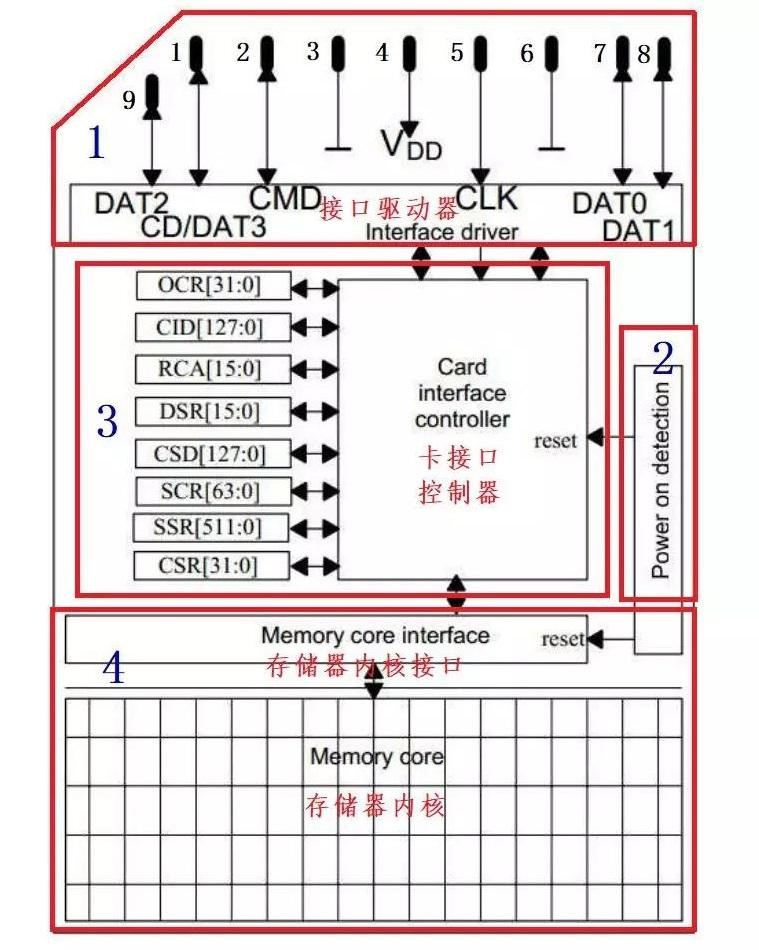
\includegraphics{figures/06-02-SD.jpg}}
    \caption{6-2-1. SD卡内部结构}
\end{figure}

SD卡内部结构如上图所示

1.3.什么是SDIO

SDIO:SDIO是在SD标准上定义了一种外设接口,它和SD卡规范间的一个重要区别是增加了低速标准。在SDIO卡只需要SPI和1位SD传输模式。低速卡的目标应用是以最小的硬件开销支持低速IO能力。

1.4.什么是MCI

MCI:MCI是Multimedia Card Interface的简称,即多媒体卡接口。上述的MMC,SD,SDI卡定义的接口都属于MCI接口。MCI这个术语在驱动程序中经常使用,很多文件,函数名字都包括”mci”.

1.5.MMC/SD/SDIO卡的区别


\begin{tabular}{|c|c|c|c|}
    
    \hline
    卡属性&引脚个数&宽度&长度&厚度&SPI传输模式&1位传输模式&时钟频率&最高传输率&最高SPI传输率\\
    \hline
    MMC卡&7&24mm&32mm&1.4mm&可选&是&否&0-20MHz&20Mbit/s&20Mbit/s \\
    \hline
    SD卡&9&24mm&32mm&2.1mm&支持&是&可选&0-25MHz&100Mbit/s&25Mbit/s \\
    \hline
    SD卡&9&24mm&32mm+&2.1mm&支持&是&可选&0-25MHz&100Mbit/s&25Mbit/s \\
    \hline
  \end{tabular}

SD卡内部有7个寄存器,如下表1所示.其中OCR,CID,CSD和SCR寄存器保存卡的配置信息;RCA寄存器保存着通信过程中卡当前暂时分配的地址(只适合SD模式);卡状态(Card Status)和SD状态(SD Status)寄存器保存着卡的状态(例如,是否写成功,通信的CRC校验是否正确等),这两个寄存器的内容与通信模式(SD模式或SPI模式)相关.MMC卡没有SCR和SD Status寄存器.

\begin{tabular}{|c|c|c|}    

    \hline
    名字 & CID & RCA & DSR & SCR & OCR &SSR &CSR \\
    \hline
    宽度 & 128 & 16 & 16 & 128 & 64 & 32 & 512 & 32 \\
    \hline
    卡识别号,每张卡都有的唯一识别号 & 发布卡的地址,卡的局部系统地址,在初始化过程中,由主机和卡动态支持 & 驱动级寄存器,配置卡的驱动输出 &
    卡的协议数据,关于卡的操作状态数据 & 卡配置寄存器,关于卡特性容量的信息 & 操作状态寄存器&
    SD状态,有关卡拥有的特性信息 & 卡状态,有关卡状态的信息 \\
    \hline
\end{tabular}

OCR寄存器保存着SD/MMC卡的供电电允许范围.如下表2所示:如果OCR寄存器的某位为1,表示卡支持该位对应的电压。最后一位表示卡上电后的状态(是否处于”忙状态”),如果该位为0,表示忙,如果为1,表示处于空闲状态(MMC/SD协议P60)。


\begin{tabular}{|c|c|}
    \hline
    OCR~bit~position&0-3&4&5&6&7&8&9&10&11&12&13&14&15&16&17&18&19&20&21&22&23&24-30&31\\
    \hline
    VDD~votage~window & Reserved & 1.6-1.7 & 1.7-1.8 & 1.8-1.9 & 1.9-2.0 & 2.0-2.1 & 2.1-2.2 & 2.2-2.3 &
    2.3-2.4 & 2.4-2.5 & 2.5-2.6 & 2.6-2.7 & 2.7-2.8 & 2.8-2.9 & 2.9-3.0 & 3.0-3.1 & 3.1-3.2 &
    3.2-3.3 & 3.3-3.4 & 3.4-3.5 & 3.5-3.6 & Reserved & Card~power~up~status~bit~(busy)1 \\
    \hline
\end{tabular}

CID为一个16个字节的寄存器,该寄存器包含一个独特的卡标识号。如下表所示:


\begin{tabular}{|c|c|c|c|}
    \hline
    Name&Manufacturer~ID&OEM/Application~ID&Product~name&Product~Revision&Product~Serial~Number&Reserved&Manufacturing~Date&CRC7~Checksum&not~used,~always~"T"\\
    \hline
Field&
MID&
OID&
PNM&
PRV&
PSN&
...&
MDT&
CRC&
-\\
    \hline
    Width&
8&
18&
40&
8&
32&
4&
12&
7&
1\\
    \hline
CID-slice&
[127:120]&
[119:104]&
[103:64]&
[83:56]&
[55:24]&
[23:20]&
[19:8]&
[7:1]&
[0:0]\\
    \hline
\end{tabular}

SD/SDIO有以下几种传输模式:
(1)SPI mode,独立序列输入和独立序列输出,使⽤CS、DI、SCLK与DO(SD卡的片选、数据输入、
时钟与数据输出)四根信号线进行数据传输。

(2)1-bit mode,独立指令和数据通道,只支持1位宽的数据传输。

(3)4-bit mode,使用额外的针脚以及某些重新设置的针脚。支持四位宽的并行传输。

6.2.2 k210联动SD卡

K210 裸机使用SD卡,下图是SD卡对应接口
\begin{figure}[H]
    \centering
    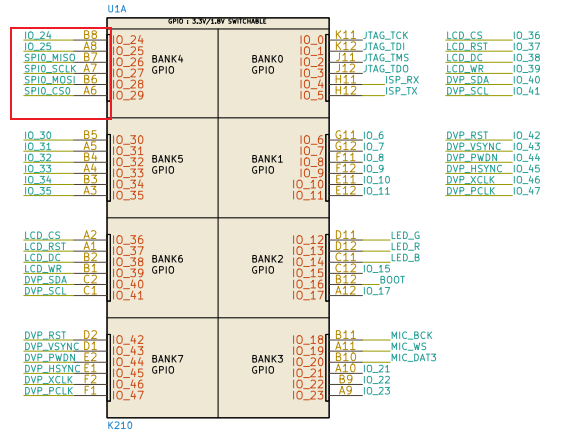
\includegraphics{figures/06-02-接口标.png}
    \caption{6-2-2. SD卡与K210接口}
\end{figure}

为了协同软硬接口,我们需要在代码中定义相关常量,使软硬接口保持一致,这即为遵守SD卡协议。
\begin{lstlisting}[language={Rust}, label={code:inode},
	caption={SD卡协议}]
    const MMIO =[
        (0x0C00_0000, 0x3000), /* PLIC */
        (0x0C20_0000, 0x1000), /* PLIC */
        (0x3800_0000, 0x1000), /* UARTHS */
        (0x3800_1000, 0x1000), /* GPIOHS */
        (0x5020_0000, 0x1000), /* GPIO */
        (0x5024_0000, 0x1000), /* SPI_SLAVE */
        (0x502B_0000, 0x1000), /* FPIOA */
        (0x502D_0000, 0x1000), /* TIMER0 */
        (0x502E_0000, 0x1000), /* TIMER1 */
        (0x502F_0000, 0x1000), /* TIMER2 */
        (0x5044_0000, 0x1000), /* SYSCTL */
        (0x5200_0000, 0x1000), /* SPI0 */
        (0x5300_0000, 0x1000), /* SPI1 */
        (0x5400_0000, 0x1000), /* SPI2 */
        ];
\end{lstlisting}


应用程序通过文件系统接口如open()、read()、write()、close()等访问文件系统,根据文件系统inode节点,接着找到文件在SD卡驱动上的块号。文件系统通过块设备驱动层与SD卡协议层对接,块设备驱动层定义了抽象块设备的接口,主要包括对块设备的读写接口。SD卡协议层主要负责按照SD卡标准规范向SD卡发送指令或者接收响应数据;硬件接口层则负责按照硬件板卡的引脚定义操作GPIO或SPI引脚实现与SD卡的数据交互。

6.2.3 SD卡的命令
 
SD卡命令共分为12类,分别为class0到Class11.
 
3.2.1. Class0 :(卡的识别、初始化等基本命令集)
CMD0:复位SD 卡。

CMD1:读OCR寄存器。

CMD9:读CSD寄存器。

CMD10:读CID寄存器。

CMD12:停止读多块时的数据传输。

CMD13:读 Card_Status 寄存器。

3.2.2.Class2 (读卡命令集):

CMD16:设置块的长度。

CMD17:读单块。

CMD18:读多块,直至主机发送CMD12为止 。
 
3.2.3.Class4(写卡命令集) :

CMD24:写单块。

CMD25:写多块。

CMD27:写CSD寄存器 。

3.2.4.Class5 (擦除卡命令集):

CMD32:设置擦除块的起始地址。

CMD33:设置擦除块的终止地址。

CMD38: 擦除所选择的块。


3.2.5.Class6(写保护命令集):

CMD28:设置写保护块的地址。

CMD29:擦除写保护块的地址。

CMD30: Ask the card for the status of the write protection bits

 class7:卡的锁定,解锁功能命令集。

 class8:申请特定命令集 。

 class10 -11 :保留。

(注:完整细节请自行参考SD卡协议官方文档)

6.2.4 SD卡工作流程

SD卡工作流程大致可以分为3个大的步骤:初始化sd卡、写sd卡、读sd卡。在SPI模式下,SD卡工作模式分为卡识别模式和数据传输模式。如下图为卡在识别模式下的命令流程。

\begin{figure}[H]
    \centering
    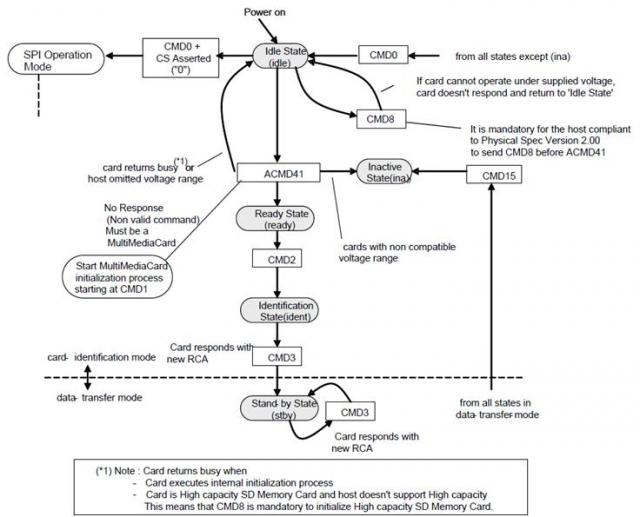
\includegraphics{figures/06-02-命令流程.png}
    \caption{6-2-3. 卡识别模式命令流程}
\end{figure}

在复位后,查找总线上的新卡的时候,主机会处于“卡识别模式”。卡在复位后会处于识别模式。不同的SD卡可能支持不同版本的协议或者不同的⼯作电压。因此,作为主机,在与SD卡进行交互之初,主机需要获取卡的工作电压范围和卡的类型。在卡识别期间,时钟频率应该保持在100~400kHZ之间。

1_在主机和SD卡进行任何通信之前,主机不知道SD卡支持的工作电压范围,卡也不知道是否支持主机当前提供的电压。因此主机首先使用默认的电压发送一条reset指令(CMD0)。

2_为了验证SD卡的接口操作状态,主机发送SEND_IF_COND(CMD8),用于取得SD卡支持工作的电压范围数据。SD卡通过检测CMD8的参数部分来检查主机使用的工作电压,主机通过分析回传的CMD8参数部分来校验SD卡是否可以在所给电压下工作,如果SD卡可以在指定电压下工作,则它回送CMD8的命令响应字 。如果不支持所给电压,则SD卡不会给出任何响应信息,并继续处于IDLE状态。

3_在发送ACMD41命令初始化高容量的SD卡前,需要强制发送CMD8命令。强制低电压主机在发送CMD8前发送ACMD41,万一双重电压SD卡没有收到CMD8命令且工作在高电压状态,在这种情况下,低电压主机不能不发送CMD8命令给卡,则收到ACMD41后进入无活动状态。

4_SD_SEND_OP_COND(ACMD)命令是为SD卡主机识别卡或者电压不匹配时拒绝卡的机制设计的。主机发送命令操作数代表要求的电压窗口大小。如果SD卡在所给的范围内不能实现数据传输,将放弃下一步的总线操作而进入无活动。操作状态寄存器也将被定义。

5_在主机发出复位命令(CMD0)后,主机将先发送CMD8再发送ACMD41命令重新初始化SD卡。

当总线被激合后,主机就开始卡的初始化和识别3处理。初始化处理设置它的操作状态和是设置OCR中的HCS比特命令SD_SEND_OP_COND(ACMD41)开始。HCS比特位被设置为1表示主机支持高容量SD卡。HCS被设置为0表示主机不支持高容量SD卡。卡的初始化和识别流程见下图。
\begin{figure}[H]
    \centering
    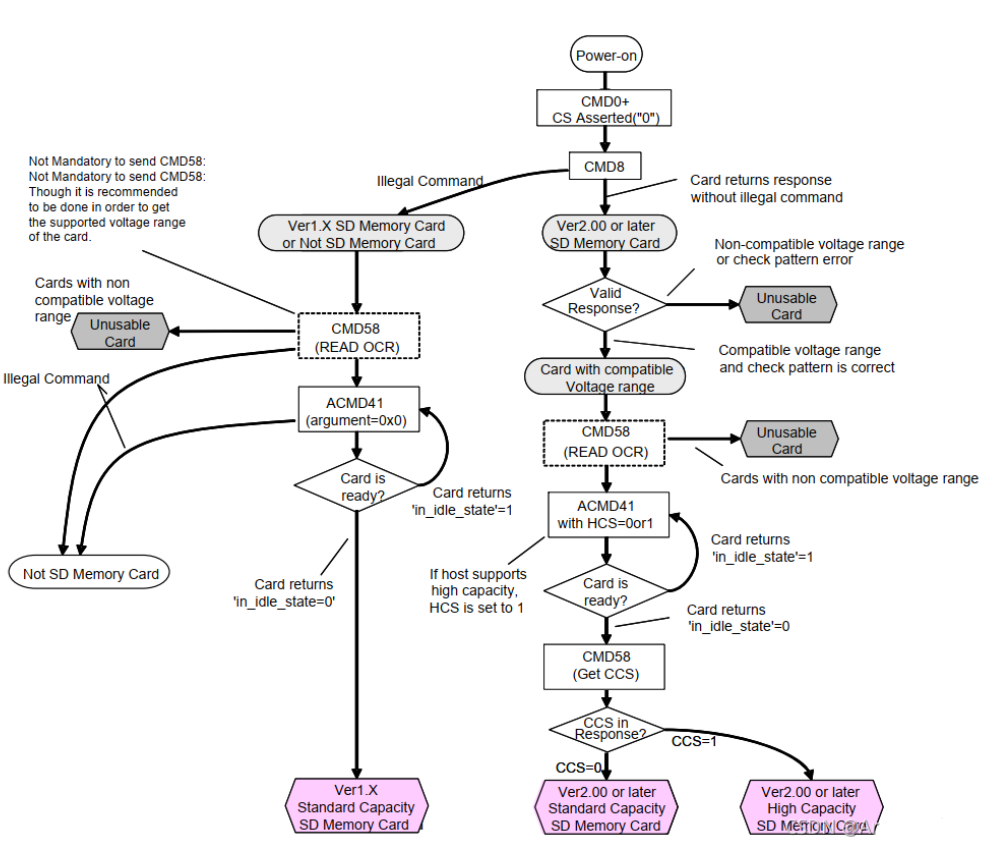
\includegraphics{figures/06-02-初始化.png}
    \caption{6-2-4. 卡初始化和识别流程}
\end{figure}
(注:这里不推荐使用NPUCore或rCore作为代码范式来讲解,应直接看SD卡协议文档)

卡在识别模式结束后,主机时钟fpp(数据传输时钟频率)将保存为fod(卡识别模式下的时钟),由于有些卡对操作时钟有限制。主机必须发送SEND_CSD(CMD9)来获得卡规格数据积存器内容,如块大小,卡容量。广播命令SET_DSR(CMD4)配置所有识别卡的驱动阶段。它对DSR积存器进行编程以适应应用总线布局,总线上的卡数目和数据传输频率。SD卡数据传输模式的流程图如下图。
\begin{figure}[H]
    \centering
    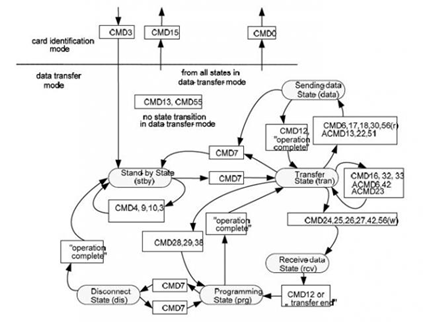
\includegraphics{figures/06-02-数据传输.png}
    \caption{6-2-5. 卡数据传输模式流程}
\end{figure}

1CMD7命令用来选择某个SD卡,使其进入Transfer状态,在指定时间段内,只有一个卡能处于Transfer状态。当某个先前被选中的处于Transfer状态的SD卡接收到CMD7之后,会释放与控制器的连接,并进入Stand-by态。当CMD7使用保留地址0x0000时,所有的SD卡都会进入Stand-by状态 。


2所有的数据读命令都可以被停止命令(CMD12)在任意时刻终止。数据传输会终止,SD卡返回Transfer状态。读命令有:块读操作(CMD17)、多块读操作(CMD18)、发送写保护(CMD30)、发送scr(ACMD51)以及读模式下的普通命令(CMD56)。

3所有的数据写命令都可以被停止命令(CMD12)在任意时刻终止。写命令也会在取消选择命令(CMD7)之前停止。写命令有:块写操作(CMD24,CMD25)、编程命令(CMD27)、锁定/解锁命令(CMD42)以及写模式下的普通命令(CMD56)。

4数据传输一旦完成,SD卡会退出数据写状态,进入Programming状态(传输成功)或者Transfer状态(传输失败)。

\section{QEMU下SD卡的驱动理解}
本节介绍在非实物环境下,使用qemu模拟SD卡块设备条件下的SD卡驱动。在qemu环境下,块设备驱动程序主要依赖virtio,本节介绍virtio标准相关内容及virtio下host和guest之间设备数据交互过程,最后使用实现该标准的第三⽅依赖库介绍npucore中QEMU下块设备驱动的实现。
随着互联网和云计算的兴起,物理服务器上通过虚拟机技术运行多个虚拟机,并在虚拟机中运行guest操作系统的模式成为主流。在传统的全虚拟化解决方案中,guest OS要使用host资源,需要Hypervisior来截获所有的请求指令,然后模拟出这些指令的行为,半虚拟化通过底层硬件辅助的方式,将部分没必要虚拟化的指令通过硬件来完成,Hypervisor只负责完成部分指令的虚拟化,guest完成不同设备的前端驱动程序,Hypervisior配合guest完成相应的后端驱动程序,两者之间通过某种交互机制实现虚拟化过程。由于不同guest前端设备其工作逻辑大同小异,单独为每个设备定义一套接口实属没有必要,而且还要考虑扩平台的兼容性问题,另外,不同后端 Hypervisor 的实现方式也类似(如KVM、Xen等)。所以,需要⼀套通用框架和标准接口(协议)来完成两者之间的交互过程。
《virtio: towards a de-facto standard for virtual I/O devices》首次提出了Virtio半虚拟化Io模型,它是⼀套通用 I/O 设备虚拟化的程序,是对半虚拟化 Hypervisor 中的⼀组通用 I/O 设备的抽象。提供了⼀套上层应⽤与各 Hypervisor 虚拟化设备(KVM,Xen,VMware等)之间的通信框架和编程接口,减少跨平台所带来的兼容性问题,大大提高驱动程序开发效率。

6.3.1 virtio架构

VirtIO由 Rusty Russell 开发,对准虚拟化 hypervisor 中的一组通用模拟设备IO的抽象。Virtio是一种前后端架构,包括前端驱动(Guest内部)、后端设备(QEMU设备)、传输协议(vring)。框架如下图所示:

 
\begin{figure}[H]
    \centering
    \scalebox{0.5}{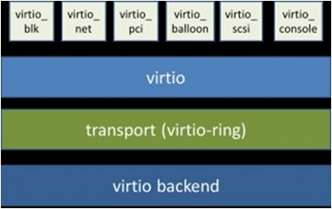
\includegraphics{figures/06-03-1.png}}
    \caption{6-3-1. virtio架构}
\end{figure}
前端驱动:

虚拟机内部的 virtio模拟设备对应的驱动。作用为接收用户态的请求,然后按照传输协议对请求进行封装,再写I/O操作,发送通知到QEMU后端设备。

后端设备:

在QEMU中创建,用来接收前端驱动发送的I/O请求,然后按照传输协议进行解析,在对物理设备进行操作,之后通过终端机制通知前端设备。

传输协议:

使用virtio队列(virtio queue,virtqueue)完成。设备有若干个队列,每个队列处理不同的数据传输(如virtio-balloon包含ivq、dvq、svq三个)。

virtqueue通过vring实现。Vring是虚拟机和QEMU之间共享的一段环形缓冲区,QEMU和前端设备都可以从vring中读取数据和放入数据。

QEMU如何感知虚拟机的操作的?虚拟机内调用kick函数实现通知之后,会产生KVM_EXIT。Host端的kvm模块捕获到这个EXIT之后,根据它退出的原因来做处理。如果是一个IO_EXIT,kvm会将这个退出交给用户态的QEMU程序来完成IO操作。

QEMU为kvm虚拟机模拟了virtio设备,因此后端的virtio-pci设备也是在QEMU进程中模拟生成的。QEMU对模拟的PCI设备的配置空间注册了回调函数,当虚拟机产生IO_EXIT,就调用这些函数来处理事件。

virtio设备通过特定于总线的方法发现和识别,每个设备由以下几个要素组成:

(1)设备状态字:设备状态字指示了在驱动程序初始化设备期间的设备状态,定义以下几个状态:

ACKNOWLEDGE(0x0000001):guest OS已找到设备,并将其识别为有效的virtio设备。

DRIVER(0x00000010):guest OS知道如何驱动设备

FAILED(0x10000000):设备出现问题。

FEATURES_OK(0x00000100):指示驱动程序以取人其所有功能

DRIVER_OK(0x00000100):指示驱动程序已设置并准备好驱动

DEVICE_NEEDS_RESET(0x01000000):指示设备需要重启。

(2)特征位:特征位用于表示virtio设备具有的各种特性和功能,其中bit0 – 23是特定设备可以使用的feature bits, bit24 – 37预给队列和feature协商机制,bit38以上保留给未来其他用途。驱动程序与设备对设备特性进行协商,形成一致的共识,这样才能正确的管理设备。

(3)通知:通知是指设备和驱动程序必须通知对方,它们有数据需要对方处理,有三种类型的通知:配置更改通知,设备->驱动程序,指示设备配置空间已更改;可用缓冲区通知,驱动程序->设备,指示缓冲区可用;已使用缓冲区通知,设备->驱动程序,指示缓冲区已经使用。

(4)设备配置空间:设备配置空间通常用于配置不常变动的设备参数(属性),或者初始化阶段需要设置的设备参数。设备的特征位中包含表示配置空间是否存在的bit位,并可通过在特征位的末尾添加新的bit位来扩展配置空间。设备驱动程序在初始化virtio设备时,需要根据virtio设备的特征位和配置空间来了解设备的特征,并对设备进行初始化。

(5)virtqueue虚拟队列

在virtio设备上进行批量数据传输的机制被称为虚拟队列(virtqueue),每个设备可以有零个或多个虚拟队列。设备驱动程序向该队列中添加缓冲区描述符并向设备发送可用缓冲区通知,通知设备从队列中读取请求;设备处理完请求后将使用的缓冲区标记为已使用并添加到队列中,向设备驱动程序发送已用缓冲区同通知,设备驱动程序从已用缓冲区中读取数据。

6.3.2 virtio块驱动整体流程

从代码上看,virtio的代码主要分两个部分:QEMU和内核驱动程序。Virtio设备的模拟就是通过QEMU完成的,QEMU代码在虚拟机启动之前,创建虚拟设备。虚拟机启动后检测到设备,调用内核的virtio设备驱动程序来加载这个virtio设备。

对于KVM虚拟机,都是通过QEMU这个用户空间程序创建的,每个KVM虚拟机都是一个QEMU进程,虚拟机的virtio设备是QEMU进程模拟的,虚拟机的内存也是从QEMU进程的地址空间内分配的。

VRING是由虚拟机virtio设备驱动创建的用于数据传输的共享内存,QEMU进程通过这块共享内存获取前端设备递交的IO请求。

如下图所示,虚拟机IO请求的整个流程:

\begin{figure}[H]
    \centering
    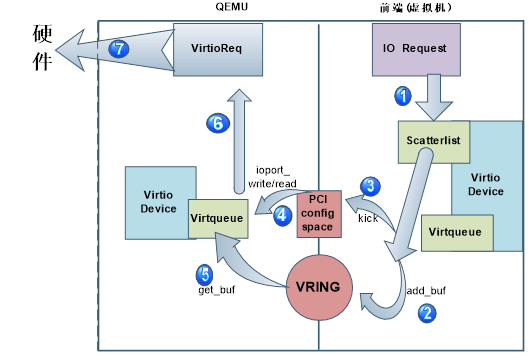
\includegraphics{figures/06-03-2.png}
    \caption{6-3-2. 虚拟机IO请求流程}
\end{figure}
1)虚拟机产生的IO请求会被前端的virtio设备接收,并存放在virtio设备散列表scatterlist里;

2)Virtio设备的virtqueue提供add_buf将散列表中的数据映射至前后端数据共享区域Vring中;

3)Virtqueue通过kick函数来通知后端qemu进程。Kick通过写pci配置空间的寄存器产生kvm_exit;

4)Qemu端注册ioport_write/read函数监听PCI配置空间的改变,获取前端的通知消息;

5)Qemu端维护的virtqueue队列从数据共享区vring中获取数据

6)Qemu将数据封装成virtioreq;

7)Qemu进程将请求发送至硬件层。

前后端主要通过PCI配置空间的寄存器完成前后端的通信,而IO请求的数据地址则存在vring中,并通过共享vring这个区域来实现IO请求数据的共享。

从上图中可以看到,Virtio设备的驱动分为前端与后端:前端是虚拟机的设备驱动程序,后端是host上的QEMU用户态程序。为了实现虚拟机中的IO请求从前端设备驱动传递到后端QEMU进程中,Virtio框架提供了两个核心机制:前后端消息通知机制和数据共享机制。

消息通知机制,前端驱动设备产生IO请求后,可以通知后端QEMU进程去获取这些IO请求,递交给硬件。

数据共享机制,前端驱动设备在虚拟机内申请一块内存区域,将这个内存区域共享给后端QEMU进程,前端的IO请求数据就放入这块共享内存区域,QEMU接收到通知消息后,直接从共享内存取数据。由于KVM虚拟机就是一个QEMU进程,虚拟机的内存都是QEMU申请和分配的,属于QEMU进程的线性地址的一部分,因此虚拟机只需将这块内存共享区域的地址传递给QEMU进程,QEMU就能直接从共享区域存取数据。下图为数据共享机制可视化图。
\begin{figure}[H]
    \centering
    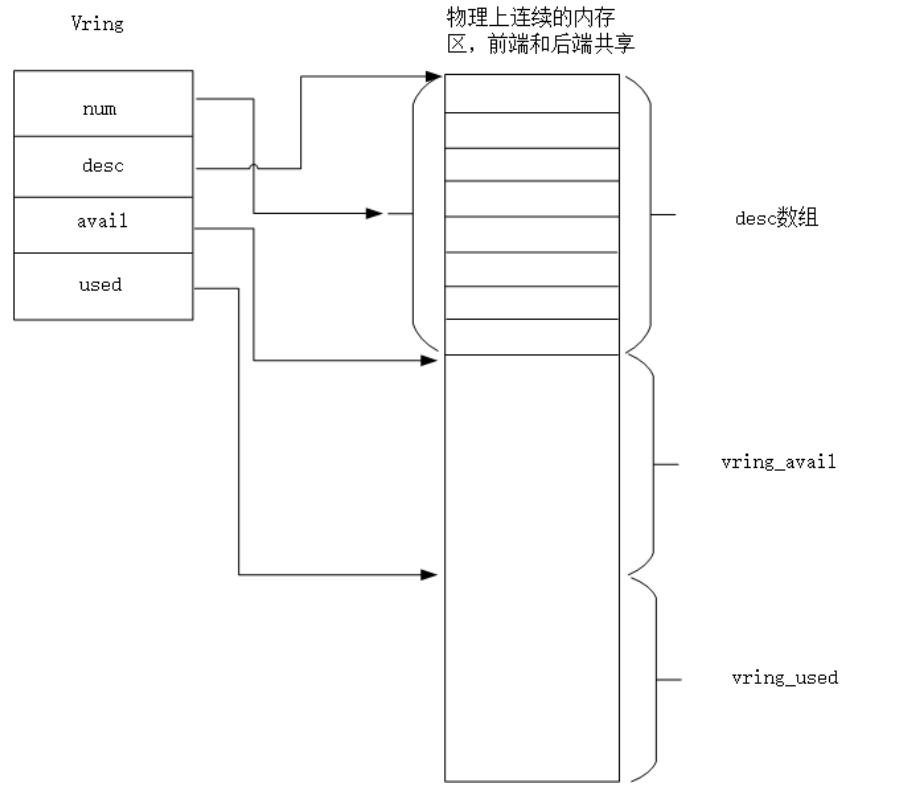
\includegraphics{figures/06-03-3.png}
    \caption{6-3-3. 数据共享机制可视化}
\end{figure}

\chapter{理解文件系统}




\section{文件系统概述}
文件最早来自于计算机用户需要把数据持久保存在 持久存储设备上的需求。由于放在内存中的数据在计算机关机或掉电后就会消失,所以应用程序要把内存中需要保存的数据放到 持久存储设备的数据块(比如磁盘的扇区等)中存起来。随着操作系统功能的增强,在操作系统的管理下,应用程序不用理解持久存储设备的硬件细节,而只需对文件这种持久存储数据的抽象进行读写就可以了,由操作系统中的文件系统和存储设备驱动程序一起来完成繁琐的持久存储设备的管理与读写。所以本章要完成的操作系统的第一个核心目标是: 让应用能够方便地把数据持久保存起来 。

对于应用程序访问持久存储设备的需求,内核需要新增两种文件:常规文件和目录文件,它们均以文件系统所维护的磁盘文件形式被组织并保存在持久存储设备上。

这里简要介绍一下在内核中添加文件系统的大致开发过程。

\textbf{第一步:是能够写出与文件访问相关的应用}

这里是参考了Linux的创建/打开/读写/关闭文件的系统调用接口,力图实现一个简化版的文件系统模型 。在用户态我们只需要遵从相关系统调用的接口约定,在用户库里完成对应的封装即可。

\textbf{第二步:实现 easyfs 文件系统}

由于 Rust 语言的特点,我们可以在用户态实现文件系统,并在用户态完成文件系统功能的基本测试并基本验证其实现正确性之后,就可以放心的将该模块嵌入到操作系统内核中。当然,有了文件系统的具体实现,还需要对上一章的操作系统内核进行扩展,实现文件系统对接的接口,这样才可以让操作系统拥有一个简单可用的文件系统。这样内核就可以支持具有文件读写功能的复杂应用。当内核进一步支持应用的命令行参数后,就可以进一步提升应用程序的灵活性,让应用的开发和调试变得更为轻松。
文件系统的整体架构自下而上可分为五层:
\begin{itemize}
    \item 磁盘块设备接口层:读写磁盘块设备的trait接口
    \item 块缓存层:位于内存的磁盘块数据缓存
    \item 磁盘数据结构层:表示磁盘文件系统的数据结构
    \item 磁盘块管理器层:实现对磁盘文件系统的管理
    \item 索引节点层:实现文件创建/文件打开/文件读写等操作
\end{itemize}
它的最底层就是对块设备的访问操作接口。两个函数 read\_block 和 write\_block ,分别代表将数据从块设备读到内存缓冲区中,或者将数据从内存缓冲区写回到块设备中,数据需要以块为单位进行读写。

尽管在操作系统的最底层(即块设备驱动程序)已经有了对块设备的读写能力,但从编程方便/正确性和读写性能的角度来看,仅有块读写这么基础的底层接口是不足以实现高效的文件系统。比如,某应用将一个块的内容读到内存缓冲区,对缓冲区进行修改,并尚未写回块设备时,如果另外一个应用再次将该块的内容读到另一个缓冲区,而不是使用已有的缓冲区,这将会造成数据不一致问题。此外还有可能增加很多不必要的块读写次数,大幅降低文件系统的性能。因此,通过程序自动而非程序员手动地对块缓冲区进行统一管理也就很必要了,该机制被我们抽象为第二层,即块缓存层。

有了块缓存,我们就可以在内存中方便地处理文件系统在磁盘上的各种数据了,这就是第三层文件系统的磁盘数据结构。

文件系统中的所有需要持久保存的数据都会放到磁盘上,这包括了管理这个文件系统的 超级块 (Super Block),管理空闲磁盘块的索引节点位图区和数据块位图区 ,以及管理文件的索引节点区和放置文件数据的数据块区组成。文件系统中管理这些磁盘数据的控制逻辑主要集中在磁盘块管理器中,这是文件系统的第四层。

对于单个文件的管理和读写的控制逻辑主要是 索引节点(文件控制块) 来完成,这是文件系统的第五层。

\textbf{第三步:把easyfs文件系统加入内核中}

这还需要做两件事情,第一件是在Qemu模拟的 virtio 块设备上实现块设备驱动程序 。由于我们可以直接使用 virtio-drivers crate中的块设备驱动,所以只要提供这个块设备驱动所需要的内存申请与释放以及虚实地址转换的4个函数就可以了。而我们之前操作系统中的虚存管理实现中,已经有这些函数,这使得块设备驱动程序很简单,且具体实现细节都被 virtio-drivers crate封装好了。

第二件事情是把文件访问相关的系统调用与easyfs文件系统连接起来。在easfs文件系统中是没有进程的概念的。而进程是程序运行过程中访问资源的管理实体,而之前的进程没有管理文件这种资源。 为此我们需要扩展进程的管理范围,把文件也纳入到进程的管理之中。 由于我们希望多个进程都能访问文件,这意味着文件有着共享的天然属性,这样自然就有了open/close/read/write这样的系统调用,便于进程通过互斥或共享方式访问文件。

内核中的进程看到的文件应该是一个便于访问的Inode,这就要对Inode 结构进一步封装,形成 OSInode 结构,以表示进程中一个打开的常规文件。而进程为了进一步管理多个文件,需要扩展文件描述符表。这样进程通过系统调用打开一个文件后,会将文件加入到自身的文件描述符表中,并进一步通过文件描述符(也就是某个特定文件在自身文件描述符表中的下标)来读写该文件。对于应用程序而言,它理解的磁盘数据是常规的文件和目录,不是 OSInode 这样相对复杂的结构。其实常规文件对应的 OSInode 是操作系统内核中的文件控制块数据结构的实例,它实现了 File Trait 定义的函数接口。这些 OSInode 实例会放入到进程文件描述符表中,并通过 sys\_read/write 系统调用来完成读写文件的服务。这样就建立了文件与 OSInode 的对应关系,通过上面描述的三个开发步骤将形成包含文件系统的操作系统内核,可给应用提供基于文件的系统调用服务。

\section{块设备接口层}
\section{buffer cache层}
\section{索引节点层}

我们使用ls -l时除了看到文件名,还看到了文件元数据
\begin{lstlisting}[]
[root@localhost linux]# ls -l
总用量 12
-rwxr-xr-x. 1 root root 7438 "9月 13 14:56" a.out
-rw-r--r--. 1 root root 654  "9月 13 14:56" test.c
\end{lstlisting}

为了能解释清楚inode我们先简单了解一下Linux的文件系统
\begin{figure}[H]
    \centering
    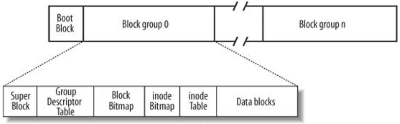
\includegraphics{figures/07-04-磁盘.png}
\end{figure}

Linux ext2文件系统,上图为磁盘文件系统图(内核内存映像肯定有所不同),磁盘是典型的块设备,硬盘分区被划分为一个个的block。一个block的大小是由格式化的时候确定的,并且不可以更改。

一个block在磁盘上的布局如下:
\begin{figure}[H]
    \centering
    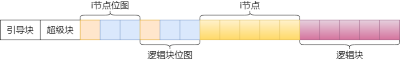
\includegraphics{figures/07-04-inode.png}
\end{figure}
由上图可知,文件系统的开头通常是由一个磁盘扇区所组成的引导块,该部分的主要目的是用于对操作系统的引导。一般只在启动操作系统时使用。
随后是超级块,超级块主要存放了该物理磁盘中文件系统结构的相关信息,并且对各个部分的大小进行说明。
inode块位图,data块位图记录了在inode块和data块中哪些块已被使用,以便找到空闲的位置
inode块和data块则是实际存放inode和数据的地方,data存放文件的内容,inode存放文件元数据并指向所属的data的地址

Linux为了对超级块,inode块,数据块这三部分进行高效的管理,Linux创建了几种不同的数据结构,分别是文件系统类型、inode、dentry等几种。
超级块反映了文件系统整体的控制信息。
dentry是反映出某个文件系统对象在全局文件系统树中的位置。
inode则反映了文件系统对象中的一般元数据信息。

\textbf{我们可以得出一个结论:inode存放了文件元数据信息,并指向文件的内容}
所以上文的`ls -l`实际上就是使用了inode的文件元数据
而npucore中虽然使用了fat32文件系统,但在代码层面上同样引入了inode这个概念,服务于文件相关系统调用的索引节点层的代码在 `vfs.rs` 中。

简单文件系统层实现了磁盘布局并能够将磁盘块有效的管理起来。但是对于文件系统的使用者而言,他们往往不关心磁盘布局是如何实现的,而是更希望能够直接看到目录树结构中逻辑上的文件和目录。为此需要设计索引节点 `Inode` ,它屏蔽了简单文件系统层对磁盘的操作,让文件系统的使用者能够直接对文件和目录进行操作。
\begin{lstlisting}[language={Rust}, label={code:inode},
	caption={easy-fs/src/fs/fat32/vfs.rs}]
pub struct Inode {
    /// Inode lock: for normal operation
    inode_lock: RwLock<InodeLock>,
    /// File Content
    file_content: RwLock<FileContent>,
    /// File cache manager corresponding to this inode.
    file_cache_mgr: PageCacheManager,
    /// File type
    file_type: Mutex<DiskInodeType>,
    /// The parent directory of this inode
    parent_dir: Mutex<Option<(Arc<Self>, u32)>>,
    /// file system
    fs: Arc<EasyFileSystem>,
    /// Struct to hold time related information
    time: Mutex<InodeTime>,
    /// Info Inode to delete file content
    deleted: Mutex<bool>,
}
\end{lstlisting}

inode\_lock: 该inode的读写锁
file\_content:指向文件的内容
file\_cache\_mgr:指向管理该inode的PageCacheManager
file\_type:文件类型
parent\_dir:指向父目录的inode以及该inode在父目录的位置
fs:指向该inode所属的简单文件系统
time:该文件的相关时间属性
delete:一个标识,控制在该inode执行析构函数时是否释放文件内容的区域

利用这个inode结构体,文件系统的使用者就可以对文件系统进行一些常用操作:
\begin{lstlisting}[language={Rust},
	caption={easy-fs/src/fs/fat32/vfs.rs}]
// 创建目录项
fn create_dir_ent(
    &self,
    inode_lock: &RwLockWriteGuard<InodeLock>,
    short_ent: FATShortDirEnt,
    long_ents: Vec<FATLongDirEnt>,
) -> Result<u32, ()>

// 删除目录项
fn delete_dir_ent(
    &self,
    inode_lock: &RwLockWriteGuard<InodeLock>,
    offset: u32,
) -> Result<(), ()>

// 创建硬链接(link)
impl Inode {
pub fn link_par_lock(
    &self,
    inode_lock: &RwLockWriteGuard<InodeLock>,
    parent_dir: &Arc<Self>,
    parent_inode_lock: &RwLockWriteGuard<InodeLock>,
    name: String,
) -> Result<(), ()>

// 删除硬链接(unlink)
pub fn unlink_lock(
    &self,
    _inode_lock: &RwLockWriteGuard<InodeLock>,
    delete: bool,
) -> Result<(), isize>
    
// ls
pub fn ls_lock(
    &self,
    inode_lock: &RwLockWriteGuard<InodeLock>,
) -> Result<Vec<(String, FATShortDirEnt)>, ()>
  
// 获取文件时间相关信息
pub fn time(&self) -> MutexGuard<InodeTime>
    
// ...
\end{lstlisting}
\section{目录和路径名}
\section{文件描述符层}
一个进程可以访问的多个文件,所以在操作系统中需要有一个管理
进程访问的多个文件的结构,这就是 \textbf{文件描述符表} (File
Descriptor Table) ,其中的每个 \textbf{文件描述符} (File Descriptor) 代
表了一个特定读写属性的I/O资源。

为简化操作系统设计实现,可以让每个进程都带有一个线性的 \textbf{文
件描述符表} ,记录该进程请求内核打开并读写的那些文件集合。
而 \textbf{文件描述符} (File Descriptor) 则是一个非负整数,表示\textbf{文件描述符表}中一个打开的\textbf{ 文件描述符} 所处的位置(可理解为数组下
标)。进程通过\textbf{文件描述符},可以在自身的\textbf{文件描述符表}中找到对
应的文件记录信息,从而也就找到了对应的文件,并对文件进行读
写。当打开( open )或创建( create ) 一个文件的时
候,一般情况下内核会返回给应用刚刚打开或创建的文件对应的文
件描述符;而当应用想关闭( close )一个文件的时候,也需
要向内核提供对应的\textbf{文件描述符},以完成对应文件相关资源的回收
操作。

因为 OSInode 也是一种要放到进程\textbf{文件描述符表}中文件,并可
通过 sys\_read/write 系统调用进行读写操作,因此我们也需
要为它实现 File Trait :
\begin{lstlisting}[language=Rust]
fn readable(&self) -> bool {
	self.readable
}
fn writable(&self) -> bool {
	self.writable
}
fn read(\&self, offset: Option<\&mut usize>, buffer: \&mut [u8]) -> usize {
	match offset {
		Some(offset) => {
			let len =
			self.inner.read_at_block_cache(*offset,
			buffer);
			*offset += len;
			len
		}
		None => {
			let mut offset =
			self.offset.lock();
			let len =
			self.inner.read_at_block_cache(*offset,
			buffer);
			*offset += len;
			len
		}
	}
}

fn write(\&self, offset: Option<\&mut
usize>, buffer: \&[u8]) -> usize {
	match offset {
		Some(offset) => {
			let len =
			self.inner.write_at_block_cache(*offset,
			buffer);
			*offset += len;
			len
		}
		None => {
			let mut offset =
			self.offset.lock();
			let inode_lock =
			self.inner.write();
			if self.append {
				*offset =
				self.inner.get_file_size_wlock(\&inode_lock)
				as usize;
			}
			let len = self
			.inner
   .write_at_block_cache_lock(\&inode_lock,
   *offset, buffer);
   *offset += len;
   len
}
}
}
\end{lstlisting}

read 将数据从文件读取到提供的缓冲区中。 offset 参数是
一个可选的 usize 的可变引用,允许指定开始读取的偏移量。如
果提供了 Some(offset) ,则从指定的偏移量开始读取,并相
应地更新偏移量。如果提供了 None ,该方法锁定偏移量,使用
当前偏移量从文件中读取数据,并相应地更新偏移量。

write 将提供的缓冲区中的数据写入文件。与 read 方法类
似,它接受一个可选的 usize 的可变引用作为偏移量参数。如果
提供了 Some(offset) ,则从指定的偏移量开始写入,并相应
地更新偏移量。如果提供了 None ,该方法锁定偏移量,获取文
件inode的写锁,然后将数据写入文件。如果设置了 append 标
志,它在写入之前将偏移量更新为文件的末尾。

同时,在NPUcore中,使用文件描述符表 Fdtable 来进行对文
件描述符的管理:

\begin{lstlisting}[language=Rust]
pub struct FdTable {
	inner: Vec<Option<FileDescriptor>>,
	recycled: Vec<u8>,
	soft_limit: usize,
	hard_limit: usize,
}
\end{lstlisting}

可以理解为文件描述符表内部存在一个向量组,我们通过open等
操作得到的文件描述符(非负整数),对应的就是该数组的下标。

\begin{lstlisting}[language=Rust]
pub struct FileDescriptor {
	cloexec: bool,
	nonblock: bool,
	pub file: Arc<dyn File>,
}
\end{lstlisting}

所以在一个进程中,活跃的文件被存放在文件描述符表中,我们通
过文件描述符表获得我们需要的文件描述符,从而找到我们需要操
作的文件,进行处理。
\section{文件相关系统调用}
npucore实现了许多POSIX规定的系统调用,本章主要介绍几个与文件相关的系统调用,包括文件的创建、打开、关闭、读写、删除等。
\subsection{write}
对于文件的读是最常使用的系统调用之一,包括输入输出都是基于终端来实现的(终端本身也可以当作一个文件)。
下面我们来介绍npucore中write的实现。

write系统调用的函数签名如下:
\begin{lstlisting}[language={C}]
int write(int fd, const void *buf, size_t count);
\end{lstlisting}
write系统调用将buf中的count个字节写入文件描述符fd所指向的文件中。成功时返回写入的字节数,失败时返回-1。

NPUCore中的代码实现如下:
\begin{lstlisting}[language={Rust}, label={lst:write}]
pub fn sys_write(fd: usize, buf: usize, count: usize) -> isize {
    let task = current_task().unwrap();
    let fd_table = task.files.lock();
    let file_descriptor = match fd_table.get_ref(fd) {
        Ok(file_descriptor) => file_descriptor,
        Err(errno) => return errno,
    };
    if !file_descriptor.writable() {
        return EBADF;
    }
    let token = task.get_user_token();
    file_descriptor.write_user(
        None,
        UserBuffer::new({
            match translated_byte_buffer(token, buf as *const u8, count) {
                Ok(buffer) => buffer,
                Err(errno) => return errno,
            }
        }),
    ) as isize
}
\end{lstlisting}
其逐代码块的解释如下:
current_task().unwrap() 获取当前任务(线程)的引用。
task.files.lock() 获取当前任务的文件表的锁,以确保并发访问的同步。
通过文件描述符 fd 从文件表中获取文件描述符的引用,使用 fd_table.get_ref(fd)。如果获取失败,则返回相应的错误号。
检查文件是否可写,如果不可写则返回 EBADF 错误号。
获取当前任务的用户令牌,通常用于在用户空间和内核空间之间传递数据。
将用户空间缓冲区的数据写入文件描述符。这里使用了 translated_byte_buffer 函数来将用户空间的字节缓冲区翻译成内核地址空间,确保正确的内存访问。
最后,将写入的字节数作为 isize 类型返回。

如果从代码的逻辑层次来分析,其调用过程如下:

sys_writet。获取当前进程的引用,然后获取文件描述符表,然后根据该表与参数fd获取对相应文件描述符的引用。这之后检查文件是否可写并获取user_token,这些操作都完成之后,以buffer(缓冲区)与count(缓冲区长度)两个参数转换为buffer,传入FileDescriptor::write_user中。

FileDescriptor::write_user。直接调用<dyn File>的write_user函数

OSInode::write_user。如果参数中offset为none(比如由write系统调用时就为none),则先获取文件偏移的锁、inode(OSInode中inner)的锁,然后看是否设置了追加标志,如果是,则将文件偏移放到最后(即从文件末尾开始写入)。然后调用OSInode.inner的write_at_block_cache_lock(即Inode::write_at_block_cache_lock)。完成之后,修改记录的文件偏移,返回写入的字节数。

Inode::write_at_block_cache_lock。内部有一个loop,计算块的末尾、写入并更新大小、移动到下一个块。到这里,写入过程就结束了。然而此时数据仍然留在内存中,还没有被持久化。被持久化的过程是另一个独立的过程,将在IO设备章节详细介绍。在这里做一个简要讲解:当满足某个条件时(比如缓冲区接近满溢),应当调用OSInode的oom函数,将满足条件的缓冲块落盘。


\subsection{read}
read函数用于从文件描述符中读取数据,并将数据存储到缓冲区中。这个系统调用在应用程序与操作系统内核之间搭建了一座桥梁,允许应用程序从指定的文件描述符中读取数据。以下是read系统调用的工作流程。

调用请求:应用程序通过执行read系统调用,并传入相应的文件描述符、缓冲区地址和要读取的字节数,发起读取请求。

参数验证:内核首先验证参数的有效性,包括文件描述符的合法性和缓冲区地址的可访问性。

读取操作:内核根据文件描述符找到相应的文件或数据流,并从中读取指定数量的字节。这个过程可能涉及文件系统的访问、网络操作或设备交互。

数据传输:读取的数据被存储在内核缓冲区中,然后被复制到用户提供的缓冲区。这个过程涉及从内核空间到用户空间的数据传输。

返回结果:read调用最终返回读取的字节数。如果到达文件末尾,则返回0。如果发生错误,则返回一个负值,并设置相应的错误码。

阻塞与非阻塞模式:read操作可以在阻塞或非阻塞模式下进行。在阻塞模式下,如果没有可用数据,read调用会阻塞调用进程,直到有数据可读。在非阻塞模式下,如果没有数据可读,read会立即返回,通常是一个错误码。

接下来是在NPUCore中read的具体实现:

\begin{lstlisting}[language=rust]
pub fn sys_read(fd: usize, buf: usize, count: usize) -> isize {
    let task = current_task().unwrap();
    let fd_table = task.files.lock();
    let file_descriptor = match fd_table.get_ref(fd) {
        Ok(file_descriptor) => file_descriptor,
        Err(errno) => return errno,
    };
    // fd is not open for reading
    if !file_descriptor.readable() {
        return EBADF;
    }
    let token = task.get_user_token();
    file_descriptor.read_user(
        None,
        UserBuffer::new({
            match translated_byte_buffer(token, buf as *const u8, count) {
                Ok(buffer) => buffer,
                Err(errno) => return errno,
            }
        }),
    ) as isize
}
\end{lstlisting}

获取当前任务:函数首先获取当前正在执行的任务或进程的上下文。

获取文件描述符表:锁定当前任务的文件描述符表,并尝试从中获取与传入的文件描述符fd相对应的文件描述符对象。

错误处理:如果指定的文件描述符不存在或其他错误发生,函数将返回相应的错误码。

检查读取权限:确认获取到的文件描述符是否具有读取权限。如果没有,返回EBADF错误码,表示文件描述符不合法或不支持读取操作。

获取用户令牌:获取与当前任务关联的用户令牌,用于后续的权限验证和内存安全检查。

处理用户缓冲区:使用$translated\_byte\_buffer$函数将用户空间的缓冲区地址和长度转换为内核可以操作的缓冲区对象UserBuffer。这一步骤涉及内存地址转换和错误检查。

执行读取操作:调用文件描述符的$read\_user$方法,从文件或数据流中读取数据到用户提供的缓冲区中。

返回结果:返回从文件描述符中实际读取的字节数。如果读取过程中发生错误,返回相应的错误码。

\subsection{open}
首先,我们分析一下NPUcore文件系统提供给应用的接口,即用户态的sys_open 系统调用。

在读写一个常规文件之前,应用首先需要通过内核提供的 sys_open 系统调用让该文件在进程的文件描述符表中占一项,并得到操作系统的返回值——文件描述符,即文件关联的表项在文件描述表中的索引值:
\begin{lstlisting}[language=rust]
// user/src/syscall.rs
/// syscall ID:56
pub fn sys_open(path: &str, flags: u32) -> isize {
	syscall(SYSCALL_OPEN, [path.as_ptr() as usize, flags as usize, 0])
}
\end{lstlisting}

如上所示 sys_open 的功能为打开一个常规文件,并返回可以访问它的文件描述符。参数path描述要打开的文件的文件名(简单起见,文件系统不需要支持目录,所有的文件都放在根目录 / 下),flags 描述打开文件的标志,具体含义下面给出。至于返回值,如果出现了错误则返回 -1,否则返回打开常规文件的文件描述符。可能的错误原因是:文件不存在。

然后我们讲解一下flags,目前我们的内核支持以下几种标志(多种不同标志可能共存):
\begin{itemize}
\item [$\bullet$]
如果 flags 为 0,则表示以只读模式 RDONLY 打开;
\item [$\bullet$]
如果 flags 第 0 位被设置(0x001),表示以只写模式 WRONLY 打开;
\item [$\bullet$]
如果 flags 第 1 位被设置(0x002),表示既可读又可写 RDWR ;
\item [$\bullet$]
如果 flags 第 9 位被设置(0x200),表示允许创建文件 CREATE ,在找不到该文件的时候应创建文件;如果该文件已经存在则应该将该文件的大小归零;
\item [$\bullet$]
如果 flags 第 10 位被设置(0x400),则在打开文件的时候应该清空文件的内容并将该文件的大小归零,也即 TRUNC 。
\end{itemize}

注意 flags 里面的权限设置只能控制进程对本次打开的文件的访问。一般情况下,在打开文件的时候首先需要经过文件系统的权限检查,比如一个文件自身不允许写入,那么进程自然也就不能以 WRONLY 或 RDWR 标志打开文件。但在我们简化版的文件系统中文件不进行权限设置,这一步就可以绕过。

在用户库 user_lib 中,我们将该系统调用封装为 open 接口:
\begin{lstlisting}[language=rust]
	// user/src/lib.rs
	
	bitflags! {
		pub struct OpenFlags: u32 {
			const RDONLY = 0;
			const WRONLY = 1 << 0;
			const RDWR = 1 << 1;
			const CREATE = 1 << 9;
			const TRUNC = 1 << 10;
		}
	}
	
	pub fn open(path: &str, flags: OpenFlags) -> isize {
		sys_open(path, flags.bits)
	}
\end{lstlisting}

如上,借助 bitflags! 宏我们将一个 u32 的 flags 包装为一个 OpenFlags 结构体更易使用,它的 bits 字段可以将自身转回 u32 ,它也会被传给 sys_open。
\begin{lstlisting}[language=rust]
	// user/src/syscall.rs
	/// syscall ID:56
	pub fn sys_open(path: &str, flags: u32) -> isize {
		syscall(SYSCALL_OPEN, [path.as_ptr() as usize, flags as usize, 0])
	}
\end{lstlisting}

如上,sys_open 传给内核的参数只有待打开文件的文件名字符串的起始地址(和之前一样,我们需要保证该字符串以 $\backslash$0 结尾)还有标志位。由于每个通用寄存器为 64 位,我们需要先将 u32 的 flags 转换为 usize 。

接下来,我们分析一下 sys_open 在内核中的实现。


\subsection{close}
首先,我们分析一下NPUcore文件系统提供给应用的接口,即用户态的 sys_close 系统调用。

在打开文件,对文件完成了读写操作后,还需要关闭文件,这样才让进程释放被这个文件占用的内核资源。 close 的调用参数是文件描述符,当文件被关闭后,该文件在内核中的资源会被释放,文件描述符会被回收。这样,进程就不能继续使用该文件描述符进行文件读写了。
\begin{lstlisting}[language=rust]
	// usr/src/lib.rs
	pub fn close(fd: usize) -> isize { sys_close(fd) }
	
	// user/src/syscall.rs
	const SYSCALL_CLOSE: usize = 57;
	
	pub fn sys_close(fd: usize) -> isize {
		syscall(SYSCALL_CLOSE, [fd, 0, 0])
	}
\end{lstlisting}

如上,sys_close 的功能是当前进程关闭一个文件,参数 fd 表示要关闭的文件的文件描述符,如果成功关闭则返回 0 ,否则返回 -1 。可能的出错原因:传入的文件描述符并不对应一个打开的文件。

接下来,我们分析一下 sys_open 在内核中的实现。

关闭文件的系统调用 sys_close 实现非常简单,我们只需将进程控制块中的文件描述符表对应的一项改为 None 代表它已经空闲即可,同时这也会导致内层的引用计数类型 Arc 被销毁,会减少一个文件的引用计数,当引用计数减少到 0 之后文件所占用的资源就会被自动回收。
\begin{lstlisting}[language=rust]
	pub fn sys_close(fd: usize) -> isize {
		info!("[sys_close] fd: {}", fd);
		let task = current_task().unwrap();
		let mut fd_table = task.files.lock();
		match fd_table.remove(fd) {
			Ok(_) => SUCCESS,
			Err(errno) => errno,
		}
	}
\end{lstlisting}

\subsection{fstat,fstatat}
NPUcore为用户提供了fstat和fstatat两个系统调用用于获取文件信息。相比之下,fstatat的功能更加完善和丰富,实现也更加复杂,这里先从fstatat开始分析。

fstatat和fstat的函数原型如下:

\begin{lstlisting}[language={Rust}, label={code:fstat,fstatat},
	caption={fstat,fstatat}]
	pub fn sys_fstatat(dirfd: usize, path: *const u8, buf: *mut u8, flags: u32) -> isize {}
	pub fn sys_fstat(fd: usize, statbuf: *mut u8) -> isize {}
		
\end{lstlisting}

从参数可以看出,statat可以按照路劲访问文件信息,而fstat则只能通过进程的文件描述符表访问。这是两者的主要区别。
对于fstat,首先进行的是获取当前进程信息以及解析路径:

\begin{lstlisting}[language={Rust}, label={code:fstatat part1},
	caption={fstatat_part1}]
    let token = current_user_token();
let path = match translated_str(token, path) {
	Ok(path) => path,
	Err(errno) => return errno,
};
let flags = match FstatatFlags::from_bits(flags) {
	Some(flags) => flags,
	None => {
		warn!("[sys_fstatat] unknown flags");
		return EINVAL;
	}
};

info!(
"[sys_fstatat] dirfd: {}, path: {:?}, flags: {:?}",
dirfd as isize, path, flags,
);

let task = current_task().unwrap();
	
\end{lstlisting}

flags这里只是进行了解析,但是在之后实现中没有涉及,这里也不过多叙述。在这里获取了当前运行的进程,并且将切片类型的path映射到当前地址空间,并且转换成string类型。

\begin{lstlisting}[language={Rust}, label={code:fstatat part2},
	caption={fstatat_part2}]
let file_descriptor = match dirfd {
	AT_FDCWD => task.fs.lock().working_inode.as_ref().clone(),
	fd => {
		let fd_table = task.files.lock();
		match fd_table.get_ref(fd) {
			Ok(file_descriptor) => file_descriptor.clone(),
			Err(errno) => return errno,
		}
	}
};

match file_descriptor.open(&path, OpenFlags::O_RDONLY, false) {
	Ok(file_descriptor) => {
		copy_to_user(token, &file_descriptor.get_stat(), buf as *mut Stat);
		SUCCESS
	}
	Err(errno) => errno,
}
\end{lstlisting}

这里先获取当前目录的文件描述符,之后调用open函数通过路径打开文件。如果文件打开成功,则调用copy_to_user函数将文件信息内容拷贝到buf中,之后函数返回。

对于文件信息的内容,NPUcore中使用结构体Stat表示,具体代码如下:
\begin{lstlisting}[language={Rust}, label={code:Stat},
	caption={Stat}]
#[derive(Clone, Copy, Debug)]
#[repr(C)]
/// Store the file attributes from a supported file.
pub struct Stat {
	/// ID of device containing file
	st_dev: u64,
	/// Inode number
	st_ino: u64,
	/// File type and mode   
	st_mode: u32,
	/// Number of hard links
	st_nlink: u32,
	/// User ID of the file's owner.
	st_uid: u32,
	/// Group ID of the file's group.
	st_gid: u32,
	/// Device ID (if special file)
	st_rdev: u64,
	__pad: u64,
	/// Size of file, in bytes.
	st_size: i64,
	/// Optimal block size for I/O.
	st_blksize: u32,
	__pad2: i32,
	/// Number 512-byte blocks allocated.
	st_blocks: u64,
	/// Backward compatibility. Used for time of last access.
	st_atime: TimeSpec,
	/// Time of last modification.
	st_mtime: TimeSpec,
	/// Time of last status change.
	st_ctime: TimeSpec,
	__unused: u64,
}
\end{lstlisting}

结构体每一个字段的含义已经给出。

对于系统调用fstat,其功能相较于fstatat更为简单。仅仅只有通过进程的文件描述符表获取文件描述符和相关信息的拷贝。具体代码如下:

\begin{lstlisting}[language={Rust}, label={code:fstat},
	caption={fstat}]
pub fn sys_fstat(fd: usize, statbuf: *mut u8) -> isize {
	let task = current_task().unwrap();
	let token = task.get_user_token();
	
	info!("[sys_fstat] fd: {}", fd);
	let file_descriptor = match fd {
		AT_FDCWD => task.fs.lock().working_inode.as_ref().clone(),
		fd => {
			let fd_table = task.files.lock();
			match fd_table.get_ref(fd) {
				Ok(file_descriptor) => file_descriptor.clone(),
				Err(errno) => return errno,
			}
		}
	};
	copy_to_user(token, &file_descriptor.get_stat(), statbuf as *mut Stat);
	SUCCESS
}
\end{lstlisting}

由于其本身传入参数的限制,fstat函数只能获取当前进程的文件信息。
\section{虚拟文件系统及接口}

\subsection{VFS简介}
虚拟文件系统(Virtual File System,简称VFS)也可称为虚拟文件转换,是一个内核软件层,用来处理与 Unix 标准文件系统相关的所有系统调用。它为用户程序提供文件和文件系统操作的统一接口,屏蔽不同文件系统的差异和操作细节。借助VFS可以直接使用open()、read()、write()这样的系统调用操作文件,而无须考虑具体的文件系统和实际的存储介质,极大简化了用户访问不同文件系统的过程。另一方面,新的文件系统、新类型的存储介质,可以无须编译的情况下,动态加载到内核中。

\begin{figure}[ht]
	\centering
	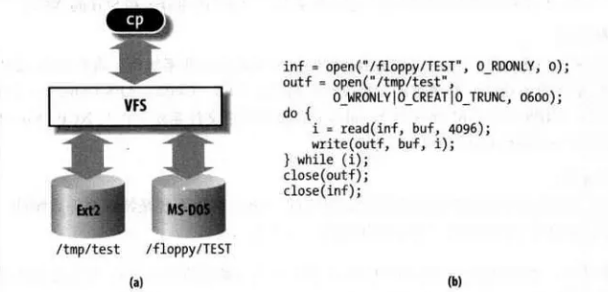
\includegraphics[width=0.5\textwidth]{figures/07-08-VFS-in-file-copy.png}
	\caption{VFS在文件复制}
	
\end{figure}

VFS的思想是把不同类型文件的共同信息放入内核,具体思路是通过在用户进程和文件系统之间引入了一个抽象层。
用户可以通过这个抽象层的接口自由使用不同的文件系统,而新的文件系统只需要支持这些接口就能直接加载到内核中使用。

\begin{figure}[ht]
	\centering
	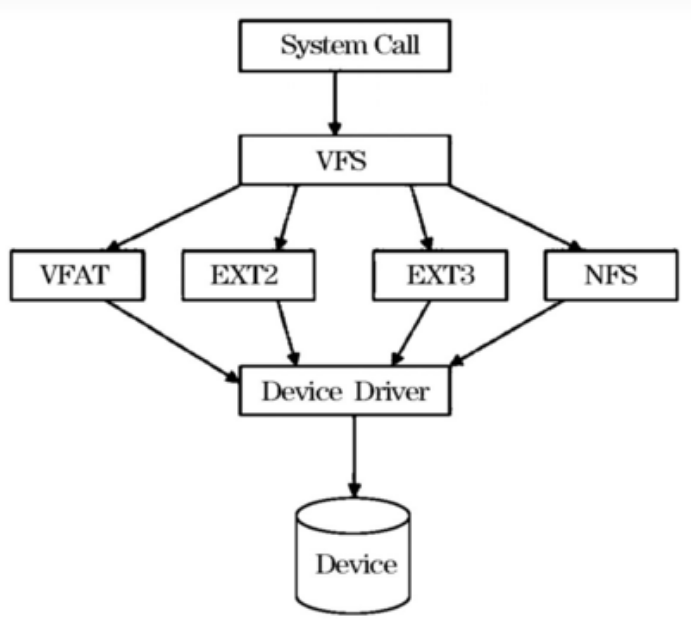
\includegraphics[width=0.5\textwidth]{figures/07-08-VFS-in-OS.png}
	\caption{VFS在OS结构中}
	
\end{figure}

\subsection{虚拟文件系统的组成}

为了实现对于不同文件系统的抽象,虚拟文件系统则需要通过数据结构完成对于不同文件系统的统一描述。在linux中为了实现这一点,定义了以下内容:

\begin{itemize}
	\item {超级块(super block)}
	超级块用于存储已安装的文件系统的相关信息。因此一个超级块可代表一个文件系统。文件系统的任意元数据修改都要修改超级块。超级块对象是常驻内
	存并被缓存的。该列表以链式方式维护在内存中,为所有进程可见。
	\item {目录项}
	目录项模块,管理路径的目录项,存储这个目录下的所有的文件的inode号和文件名等信息。其内部是
	树形结构,操作系统检索一个文件,都是从根目录开始,按层次解析路径中的所有目录,直到定位到
	文件。
	\item {inode}
	存放具体文件的一般信息(内核在操作文件或目录时需要的全部信息)。一个索引节点代表文件系统中的一个文件,但是索引节点仅当文件被访问时,才在内存中创建
	\item {文件对象}
	它代表由进程打开的文件。存放打开文件与进程之间进行交互的有关信息。这些信息仅当进程访问文件期间存放在内核中。
	这类信息仅当进程访问期间存在于内核内存中。文件对象(不是物理文件)由相应的open()系统调用创建,由close()系统调用撤销。
\end{itemize}

在NPUcore中,各部分由相应的数据结构实现。

对于超级块,NPUcore中在虚拟文件系统中定义了一个filesystem结构体,用来存储文件系统的信息。这个结构体较为简单。由于NPUcore暂时只支持FAT32文件系统,所以文件系统的类型的枚举类型只有两个值。
具体代码如下:

\begin{lstlisting}[language={Rust},caption={filesystem}]
	pub enum FS {
		Null,
		Fat32,
	}
	
	pub struct FileSystem {
		pub fs_id: usize,
		pub fs_type: FS,
	}
\end{lstlisting}

对于目录项和inode,NPUcore使用了DirectoryTreeNode结构体。不难发现,这里既有相关目录的下文件的部分,又有相关文件的信息。定义如下:

\begin{lstlisting}[language={Rust}, caption={DirectoryTreeNode}]
	pub struct DirectoryTreeNode {
		/// If this is a directory
		/// 1. cwd
		/// 2. mount point
		/// 3. root node
		/// If this is a file
		/// 1. executed by some processes
		/// This parameter will add 1 when opening
		spe_usage: Mutex<usize>,
		name: String,
		filesystem: Arc<FileSystem>,
		file: Arc<dyn File>,
		selfptr: Mutex<Weak<Self>>,
		father: Mutex<Weak<Self>>,
		children: RwLock<Option<BTreeMap<String, Arc<Self>>>>,
	}
\end{lstlisting}

从结构可以看出,这里实现了一个树形结构,指向子节点并带有路径,同时还有指向文件和文件系统的Arc指针。

对于文件对象,使用了文件描述符file\_description。定义如下:

\begin{lstlisting}[language={Rust},caption={DirectoryTreeNode}]
	#[derive(Clone)]
	pub struct FileDescriptor {
		cloexec: bool,
		nonblock: bool,
		pub file: Arc<dyn File>,
	}
\end{lstlisting}

从表面上看这些和多文件系统共存没有关系,但是以下代码完成了该项功能:
\begin{lstlisting}[language={Rust}, caption={file\_trait}]
	pub trait File: DowncastSync {
		fn deep_clone(&self) -> Arc<dyn File>;
		fn readable(&self) -> bool;
		fn writable(&self) -> bool;
		fn read(&self, offset: Option<&mut usize>, buf: &mut [u8]) -> usize;
		fn write(&self, offset: Option<&mut usize>, buf: &[u8]) -> usize;
		fn r_ready(&self) -> bool;
		fn w_ready(&self) -> bool;
		fn read_user(&self, offset: Option<usize>, buf: UserBuffer) -> usize;
		fn write_user(&self, offset: Option<usize>, buf: UserBuffer) -> usize;
		fn get_size(&self) -> usize;
		fn get_stat(&self) -> Stat;
		fn get_file_type(&self) -> DiskInodeType;
		fn is_dir(&self) -> bool {
			self.get_file_type() == DiskInodeType::Directory
		}
		fn is_file(&self) -> bool {
			self.get_file_type() == DiskInodeType::File
		}
		fn info_dirtree_node(&self, dirnode_ptr: Weak<DirectoryTreeNode>);
		fn get_dirtree_node(&self) -> Option<Arc<DirectoryTreeNode>>;
		/// open
		fn open(&self, flags: OpenFlags, special_use: bool) -> Arc<dyn File>;
		fn open_subfile(&self) -> Result<Vec<(String, Arc<dyn File>)>, isize>;
		/// create
		fn create(&self, name: &str, file_type: DiskInodeType) -> Result<Arc<dyn File>, isize>;
		fn link_child(&self, name: &str, child: &Self) -> Result<(), isize>
		where
		Self: Sized;
		/// delete(unlink)
		fn unlink(&self, delete: bool) -> Result<(), isize>;
		/// dirent
		fn get_dirent(&self, count: usize) -> Vec<Dirent>;
		/// offset
		fn get_offset(&self) -> usize {
			self.lseek(0, SeekWhence::SEEK_CUR).unwrap()
		}
		fn lseek(&self, offset: isize, whence: SeekWhence) -> Result<usize, isize>;
		/// size
		fn modify_size(&self, diff: isize) -> Result<(), isize>;
		fn truncate_size(&self, new_size: usize) -> Result<(), isize>;
		// time
		fn set_timestamp(&self, ctime: Option<usize>, atime: Option<usize>, mtime: Option<usize>);
		/// cache
		fn get_single_cache(&self, offset: usize) -> Result<Arc<Mutex<PageCache>>, ()>;
		fn get_all_caches(&self) -> Result<Vec<Arc<Mutex<PageCache>>>, ()>;
		/// memory related
		fn oom(&self) -> usize;
		/// poll, select related
		fn hang_up(&self) -> bool;
		/// iotcl
		fn ioctl(&self, _cmd: u32, _argp: usize) -> isize {
			ENOTTY
		}
		/// fcntl
		fn fcntl(&self, cmd: u32, arg: u32) -> isize;
	}
\end{lstlisting}

这在rust语法中属于特性,可以实现泛型。无论文件系统的文件结构如何定义,只要实现了这些特性,虚拟文件系统就可以识别并进行操作,很好地完成了这一点。这里不得不感叹rust语法的巧妙所在。

\subsection{虚拟文件系统提供的接口}

\begin{itemize}
	\item \texttt{sys\_openat}: 
	\begin{lstlisting}[language=rust]
		pub fn sys_openat(dirfd: usize, path: *const u8, flags: u32, mode: u32)
	\end{lstlisting}
	该接口接收来自用户空间的参数,包括目录描述符 dirfd、路径 path、打开标志位 flags 和文件权限 mode。它会根据传入的目录描述符选择要打开的文件描述符,并通过文件描述符的 open() 方法尝试打开文件。如果打开失败,则返回相应的错误码。然后,函数将新打开的文件描述符插入到当前任务的文件描述符表中,并返回新文件描述符的整数值
	\item \texttt{sys\_close}: 
	\begin{lstlisting}[language=rust]
		pub fn sys_close(fd: usize)
	\end{lstlisting}
	该接口会将进程控制块中的文件描述符表对应的一项改为 None ,代表它已经空闲,同时这也会导致内层的引用计数类型 Arc 被销毁,会减少一个文件的引用计数,当引用计数减少到 0 之后文件所占用的资源就会被自动回收。
	\item \texttt{sys\_read}: 
	\begin{lstlisting}[language=rust]
		pub fn sys_read(fd: usize, buf: usize, count: usize)
	\end{lstlisting}
	该接口根据文件描述符 fd 在文件描述符表中找到相应的文件描述符对象,使用文件描述符的 read\_user() 方法尝试从文件中读取数据到用户空间的缓冲区 buf 中,读取count个字节。
	\item \texttt{sys\_write}: 
	\begin{lstlisting}[language=rust]
		pub fn sys_write(fd: usize, buf: usize, count: usize)
	\end{lstlisting}
	该接口根据文件描述符 fd 在文件描述符表中找到相应的文件描述符对象,使用文件描述符的 write\_user() 方法尝试从文件中写入数据到用户空间的缓冲区 buf 中,共写count个字节。
	\item \texttt{sys\_fstat}: 
	\begin{lstlisting}[language=rust]
		pub fn sys_fstat(fd: usize, statbuf: *mut u8)
	\end{lstlisting}
	该接口根据文件描述符 fd 在文件描述符表中找到相应的文件描述符对象,并根据文件描述符提供的方法将文件信息写入缓冲区 statbuf 中。
	\item \texttt{sys\_mount}: 
	\begin{lstlisting}[language=rust]
		pub fn sys_mount(source: *const u8,target: *const u8,filesystemtype: *const u8,mountflags: usize,data: *const u8,)
	\end{lstlisting}
	该接口实现了挂载,参数中 source 为要挂载的文件系统的源路径或标识,target 为文件系统将要挂载到的目标位置,filesystemtype 为要挂载的文件系统的类型,mountflags是挂载选项和标志,data 为挂载所需的其他数据。
	\item \texttt{sys\_lseek}: 
	\begin{lstlisting}[language=rust]
		pub fn sys_lseek(fd: usize, offset: isize, whence: u32)
	\end{lstlisting}
	该接口根据文件描述符 fd 在文件描述符表中找到相应的文件描述符对象,然后以 whence 为偏移的基准,offset 为偏移量,返回操作后的文件指针位置。
	\item \texttt{sys\_mkdirat}: 
	\begin{lstlisting}[language=rust]
		pub fn sys_mkdirat(dirfd: usize, path: *const u8, mode: u32)
	\end{lstlisting}
	该接口在指定路径 dirfd 下创建路径为 path 的目录。
\end{itemize}
\section{文件共享与PIPE}
文件共享和管道是操作系统中关键的概念,它们为进程之间的通信和协同提供了有效的手段。
在npucore中,这些机制是构建多任务、多进程应用程序的基础。本章将深入探讨文件共享和管道的原理、应用和在npucore中的具体实现。

文件共享是多个进程之间共享数据的一种机制。
我们将深入研究硬链接和软链接,它们分别提供了对同一文件的不同访问方式。

硬链接是文件系统中的重要概念,允许一个文件存在于多个位置,节省存储空间并提供数据的共享。
与硬链接相比,软链接提供了更灵活的方式来共享文件。

文件描述符是在进程和文件之间建立联系的关键。
文件共享不仅仅是为了在同一进程内部使用,还可以用于不同进程之间的通信。在实际的运用场景中,我们常常需要在父子进程之间通信,POSIX提供了一种特殊的文件描述符,可以用于实现这种通信,叫做管道。
管道是一种强大的进程通信工具,使得不同进程之间能够直接传递数据。我们将深入研究管道的工作原理,以及在 xv6 中如何创建、使用管道。
在了解了管道的基本概念后,我们将深入研究在npucore中如何创建和使用管道。这涉及到管道的创建、连接和断开的具体步骤。
管道不仅仅是用于数据传输,还促进了进程之间的通信。我们将说明在npucore中如何利用管道实现进程间通信,以及这种通信的应用场景。
通过深入研究这些主题,读者将能够全面了解在npucore操作系统中如何利用文件共享和管道机制来构建灵活、高效的多任务应用程序。

\subsection{软链接与硬链接}

\section{硬链接和软链接}
连接分为两种类型:硬链接(hard link)和软链接(symbolic link)。
本文将详细介绍这两种类型的连接的特点、用法和区别。
硬链接是指在同一个文件系统中,将一个文件名关联到一个已经存在的文件上,使得该文件名也可以访问该文件。硬链接与原文件共享inode,即它们有相同的inode号和相同的device号。因此,对于硬链接和原文件来说,它们的访问权限、所有者、大小等属性都是相同的。
软链接(也称符号链接)是指在不同的文件系统之间,将一个文件名关联到另一个文件上,使得该文件名也可以访问该文件。软链接与原文件不共享inode,它们有不同的inode号和device号。因此,对于软链接和原文件来说,它们的访问权限、所有者、大小等属性可能不同。
\subsection{硬链接}
硬链接是指一个文件系统中的多个文件名指向同一个数据块(inode)的情况。也就是说,硬链接是同一个文件的不同别名,它们共享相同的内容,属性和权限。硬链接只能在同一个分区内创建,不能跨越不同的文件系统。
硬链接是通过在文件系统中创建一个新的目录项来实现的,这个目录项指向同一个 inode,即原始文件的 inode。在文件系统中,每个文件和目录都有一个 inode,它包含了文件的元数据信息和数据块的位置信息。

当创建一个硬链接时,文件系统会在相应的目录中创建一个新的目录项,这个目录项与原始文件的 inode 相关联,因此它们实际上是同一个文件,只是有不同的文件名和目录路径。

由于硬链接与原始文件共享相同的 inode,它们实际上是同一个文件,因此它们具有相同的权限、所有者、所属组、创建时间、修改时间等。这意味着,如果您修改硬链接文件的内容,那么原始文件的内容也会被修改,因为它们指向相同的 inode。

当删除一个硬链接时,它只是将相应的目录项从文件系统中删除,但是原始文件的 inode 仍然存在,并且只有当所有的硬链接都被删除时,该 inode 才会被释放,文件才会被删除。

总之,硬链接的实现原理是通过在文件系统中创建一个新的目录项,并将其与原始文件的 inode 号和文件内容进行关联,从而实现多个文件名指向同一个文件的效果。

需要注意的是,硬链接只能在同一个文件系统中创建,因为它们都指向相同的 inode。如果您尝试在不同的文件系统中创建硬链接,那么会创建一个新的文件副本,而不是一个硬链接。

以下代码将具体讲解在NPUCore中Link的实现方式:

\begin{lstlisting}[language=rust]
pub fn sys_linkat(
    old_dirfd: usize,
    old_path: *const u8,
    new_dirfd: usize,
    new_path: *const u8,
    flags: u32,
) -> isize {
    let task = current_task().unwrap();
    let token = task.get_user_token();
    let old_path = match translated_str(token, old_path) {
        Ok(path) => path,
        Err(errno) => return errno,
    };
    let new_path = match translated_str(token, new_path) {
        Ok(path) => path,
        Err(errno) => return errno,
    };
    info!(
        "[sys_linkat] old_dirfd: {}, old_path: {}, new_dirfd: {}, new_path: {}, flags: {:?}",
        old_dirfd as isize, old_path, new_dirfd as isize, new_path, flags
    );

    let old_file_descriptor = match old_dirfd {
        AT_FDCWD => task.fs.lock().working_inode.as_ref().clone(),
        fd => {
            let fd_table = task.files.lock();
            match fd_table.get_ref(fd as usize) {
                Ok(file_descriptor) => file_descriptor.clone(),
                Err(errno) => return errno,
            }
        }
    };

    // let old_inode = old_file_descriptor.file.deep_clone();

    let new_file_descriptor = match new_dirfd {
        AT_FDCWD => task.fs.lock().working_inode.as_ref().clone(),
        fd => {
            let fd_table = task.files.lock();
            match fd_table.get_ref(fd as usize) {
                Ok(file_descriptor) => file_descriptor.clone(),
                Err(errno) => return errno,
            }
        }
    };

    match FileDescriptor::linkat(
        &old_file_descriptor,
        &old_path,
        &new_file_descriptor,
        &new_path,
    ) {
        Ok(_) => SUCCESS,
        Err(errno) => errno,
    }
}
\end{lstlisting}

$\texttt{old\_dirfd}$和$\texttt{new\_dirfd}$:这两个参数是文件目录的文件描述符,分别指向旧文件和新链接文件所在的目录。
$\texttt{old\_path}$和$\texttt{new\_path}$:这是指向旧文件和新链接文件路径的指针。
$flags$:这是一个控制函数行为的标志位,用于提供额外的操作信息。

获取当前任务上下文:函数首先获取当前正在执行的任务(或进程)的上下文,这对于后续的文件操作是必要的。

用户令牌获取:为了确保操作的安全性,函数获取了与当前任务关联的用户令牌。

路径转换:将$\texttt{old\_path}$和$\texttt{new\_path}$从原始的指针形式转换为Rust语言中的字符串形式。这一步骤涉及内存安全和权限的考虑。

日志记录:为了便于调试和跟踪,函数记录了关键的操作信息。

处理文件描述符:函数根据传入的$\texttt{old\_dirfd}$和$\texttt{new\_dirfd}$获取相应的文件描述符。这里的处理包括判断文件描述符是否代表当前工作目录($AT\_FDCWD$),以及从文件描述符表中获取相应的文件描述符对象。

链接创建:最后,函数调用特定的方法(FileDescriptor)来在文件系统中创建链接。这涉及到检查文件权限、管理文件系统的inode,以及确保链接创建的正确性。

错误处理和返回值:整个函数在执行过程中,会对可能出现的错误情况进行处理。成功执行后返回特定的成功值(如0),失败则返回相应的错误码。

\begin{lstlisting}[language=rust]
pub fn linkat(
        old_fd: &Self,
        old_path: &str,
        new_fd: &Self,
        new_path: &str,
    ) -> Result<(), isize> {
        if old_fd.file.is_file() && !old_path.starts_with('/') {
            return Err(ENOTDIR);
        }
        if new_fd.file.is_file() && !new_path.starts_with('/') {
            return Err(ENOTDIR);
        }
        let old_inode = old_fd.file.get_dirtree_node();
        let old_inode = match old_inode {
            Some(inode) => inode,
            None => return Err(ENOENT),
        };
        let new_inode = new_fd.file.get_dirtree_node();
        let new_inode = match new_inode {
            Some(inode) => inode,
            None => return Err(ENOENT),
        };

        let mut old_abs_path = [old_inode.get_cwd(), old_path.to_string()].join("/");
        if old_path.starts_with('/') {
            old_abs_path = old_path.to_string();
        } else {
            old_abs_path = [old_inode.get_cwd(), old_path.to_string()].join("/");
        }
        let mut new_abs_path = [new_inode.get_cwd(), new_path.to_string()].join("/");
        if new_path.starts_with('/') {
            new_abs_path = new_path.to_string();
        } else {
            new_abs_path = [new_inode.get_cwd(), new_path.to_string()].join("/");
        }
        //println!("link_path: {} -> {}", old_path, new_path);
        //println!("link_abs: {} -> {}", old_abs_path, new_abs_path);
        DirectoryTreeNode::linkat(&old_abs_path, &new_abs_path)
    }
\end{lstlisting}

参数验证:首先检查旧文件描述符和新文件描述符。函数验证这两个描述符是否指向有效的文件(而非目录),同时检查提供的路径是否以斜杠(/)开头。如果任一路径不符合条件,函数将返回错误。

获取inode节点:对于旧文件和新文件的路径,函数获取它们各自的inode节点。inode是文件系统中用于存储文件属性的数据结构。如果无法获取inode节点,函数返回错误。

路径处理:函数根据旧文件和新文件的inode节点以及提供的路径,生成完整的绝对路径。如果提供的路径已经是绝对路径(即以斜杠开头),则直接使用该路径。否则,将inode节点的当前工作目录与提供的路径结合生成绝对路径。

创建链接:最后,函数尝试在文件系统中创建一个从旧文件到新文件位置的链接。这是通过调用特定的方法实现的。

结果返回:如果链接创建成功,函数返回成功的结果;如果失败,则返回相应的错误码。

\begin{lstlisting}[language=rust]
pub fn linkat(old_path: &str, new_path: &str) -> Result<(), isize> {
        assert!(old_path.starts_with('/'));
        assert!(new_path.starts_with('/'));

        let mut old_comps = Self::parse_dir_path(old_path);
        let mut new_comps = Self::parse_dir_path(new_path);

        // We gurantee that last component isn't empty
        let old_last_comp = old_comps.pop().unwrap();
        let new_last_comp = new_comps.pop().unwrap();

        let old_par_inode = match ROOT.cd_comp(&old_comps) {
            Ok(inode) => inode,
            Err(errno) => return Err(errno),
        };
        let new_par_inode = match ROOT.cd_comp(&new_comps) {
            Ok(inode) => inode,
            Err(errno) => return Err(errno),
        };
        type ChildLockType<'a> =
            RwLockWriteGuard<'a, Option<BTreeMap<String, Arc<DirectoryTreeNode>>>>;

        let old_lock: Arc<Mutex<ChildLockType<'_>>>;
        let new_lock: Arc<Mutex<ChildLockType<'_>>>;

        // Be careful about the lock ordering
        if old_comps == new_comps {
            old_lock = Arc::new(Mutex::new(old_par_inode.children.write()));
            new_lock = old_lock.clone();
        } else if old_comps < new_comps {
            old_lock = Arc::new(Mutex::new(old_par_inode.children.write()));
            new_lock = Arc::new(Mutex::new(new_par_inode.children.write()));
        } else {
            new_lock = Arc::new(Mutex::new(new_par_inode.children.write()));
            old_lock = Arc::new(Mutex::new(old_par_inode.children.write()));
        }

        let old_inode =
            match old_par_inode.try_to_open_subfile(old_last_comp, &mut (*old_lock.lock())) {
                Ok(inode) => inode,
                Err(errno) => return Err(errno),
            };

        if *old_inode.spe_usage.lock() > 0 {
            return Err(EBUSY);
        }

        if old_inode.filesystem.fs_id != new_par_inode.filesystem.fs_id {
            return Err(EXDEV);
        }
        let old_key = old_last_comp.to_string();
        let new_key = new_last_comp.to_string();
        match new_par_inode.try_to_open_subfile(new_last_comp, &mut (*new_lock.lock())) {
            Ok(new_inode) => {
                if new_inode.file.is_dir() && !old_inode.file.is_dir() {
                    return Err(EISDIR);
                }
                if old_inode.file.is_dir() && !new_inode.file.is_dir() {
                    return Err(ENOTDIR);
                }
                if *new_inode.spe_usage.lock() > 0 {
                    return Err(EBUSY);
                }
                // delete
                return Err(EEXIST);
            }
            Err(ENOENT) => {}
            Err(errno) => return Err(errno),
        }

        match old_inode.filesystem.fs_type {
            FS::Fat32 => {
                let old_file = old_inode.file.downcast_ref::<OSInode>().unwrap();
                let new_par_file = new_par_inode.file.downcast_ref::<OSInode>().unwrap();
                new_par_file.link_child(new_last_comp, old_file)?;
            }
            FS::Null => return Err(EACCES),
        }

        let value = old_lock.lock().as_mut().unwrap().get(&old_key).unwrap().clone();
        let new_value = DirectoryTreeNode::new(
            new_key.clone(),
            new_par_inode.filesystem.clone(),
            value.file.deep_clone(),
            Arc::downgrade(&new_par_inode.get_arc()),
        );
        new_lock.lock().as_mut().unwrap().insert(new_key, new_value);
        Ok(())
    }
\end{lstlisting}

路径验证:首先检查$old\_path$和$new\_path$是否都是以斜杠(/)开头的绝对路径。这是通过断言(assert!)来完成的。

解析路径:函数将旧路径和新路径解析为它们的组成部分。

获取父inode:接下来,函数查找旧路径和新路径的父inode(索引节点),这是文件系统中存储文件元数据的结构。

锁定处理:为了线程安全,函数对父inode的子节点进行锁定。如果旧路径和新路径的父节点相同,它们将共享同一个锁;否则,会分别获得各自的锁。

打开子文件:函数尝试打开旧路径的子文件,并对特定的使用情况进行检查,例如是否正被使用(EBUSY错误)。

文件系统一致性检查:检查旧路径和新路径是否位于同一个文件系统上。如果不是,返回错误(EXDEV)。

链接创建:根据文件系统的类型(如FS::Fat32),执行特定的链接创建操作。如果是不支持的文件系统类型,则返回错误(EACCES)。

处理新路径下的文件:如果新路径下已存在文件,根据文件类型(目录或普通文件)进行错误检查,并处理可能的冲突。

更新子节点:最后,更新新路径的父inode的子节点映射,以包含新创建的链接。

返回结果:根据上述步骤的执行情况,函数返回成功或相应的错误码。

讲完上面硬链接的实现,我们现在来讲一下如何删除一个链接。在NPUCore中删除一个链接,我们直接删除新链接的文件即可。下面是在NPUCore中具体实现:

\begin{lstlisting}[language=rust]
pub fn sys_unlinkat(dirfd: usize, path: *const u8, flags: u32) -> isize {
    let task = current_task().unwrap();
    let token = task.get_user_token();
    let path = match translated_str(token, path) {
        Ok(path) => path,
        Err(errno) => return errno,
    };
    let flags = match UnlinkatFlags::from_bits(flags) {
        Some(flags) => flags,
        None => {
            warn!("[sys_unlinkat] unknown flags");
            return EINVAL;
        }
    };
    info!(
        "[sys_unlinkat] dirfd: {}, path: {}, flags: {:?}",
        dirfd as isize, path, flags
    );

    let file_descriptor = match dirfd {
        AT_FDCWD => task.fs.lock().working_inode.as_ref().clone(),
        fd => {
            let fd_table = task.files.lock();
            match fd_table.get_ref(fd) {
                Ok(file_descriptor) => file_descriptor.clone(),
                Err(errno) => return errno,
            }
        }
    };
    match file_descriptor.delete(&path, flags.contains(UnlinkatFlags::AT_REMOVEDIR)) {
        Ok(_) => SUCCESS,
        Err(errno) => errno,
    }
}
\end{lstlisting}

获取当前任务:函数首先获取当前执行的任务或进程的上下文。

用户令牌获取:获取与当前任务关联的用户令牌,这对于接下来的文件操作是必要的。

路径转换:将path参数从原始指针转换为Rust字符串。这一步骤涉及权限验证和内存安全。

标志位处理:解析传入的flags参数,将其转换为适当的标志位集合。如果标志位未知,记录警告信息并返回错误。

日志记录:记录操作的关键信息,包括目录文件描述符、路径和标志位。

处理文件描述符:根据传入的dirfd获取相应的文件描述符。如果dirfd是特殊值(如$AT\_FDCWD$,表示当前工作目录),则使用当前任务的工作inode;否则,从文件描述符表中获取对应的文件描述符。

执行删除操作:调用文件描述符的删除方法,根据路径和标志位执行删除操作。如果标志位包含特定值(如$AT\_REMOVEDIR$),则执行目录的删除;否则,删除文件。

返回结果:根据删除操作的结果返回相应的状态码。成功执行返回特定的成功值(如0),失败则返回相应的错误码。

\begin{lstlisting}[language=rust]
    pub fn delete(&self, path: &str, delete_directory: bool) -> Result<(), isize> {
        if self.file.is_file() && !path.starts_with('/') {
            return Err(ENOTDIR);
        }
        let inode = self.file.get_dirtree_node();
        let inode = match inode {
            Some(inode) => inode,
            None => return Err(ENOENT),
        };
        inode.delete(path, delete_directory)
    }
\end{lstlisting}

路径验证:首先检查是否当前对象(self)代表的是一个文件,并且传入的路径(path)是否是绝对路径(以/开头)。如果不是绝对路径,且当前对象是文件,则返回ENOTDIR错误,表示路径不是一个目录。

获取inode节点:函数尝试获取当前文件对象的inode节点。inode是文件系统中用于存储文件元数据的结构。如果无法获取inode节点,函数返回ENOENT错误,表示文件或目录不存在。

调用删除操作:通过inode节点,函数调用删除操作。这个操作将根据path参数和$delete\_directory$参数来决定具体的删除行为。如果$delete\_directory$为true,则尝试删除目录;否则,删除文件。

返回结果:根据删除操作的结果,函数返回成功或错误状态。如果操作成功执行,返回Ok(());如果有错误发生,返回对应的错误码。

\begin{lstlisting}[language=rust]
pub fn delete(&self, path: &str, delete_directory: bool) -> Result<(), isize> {
        if path.split('/').last().map_or(true, |x| x == ".") {
            return Err(EINVAL);
        }

        let inode = if path.starts_with("/") {
            &**ROOT
        } else {
            &self
        };

        let components = Self::parse_dir_path(path);
        let last_comp = *components.last().unwrap();
        let inode = match inode.cd_comp(&components) {
            Ok(inode) => inode,
            Err(errno) => return Err(errno),
        };

        if *inode.spe_usage.lock() > 0 {
            return Err(EBUSY);
        }

        if !delete_directory && inode.file.is_dir() {
            return Err(EISDIR);
        }

        if delete_directory && !inode.file.is_dir() {
            return Err(ENOTDIR);
        }

        match inode.father.lock().upgrade() {
            Some(par_inode) => {
                let mut lock = par_inode.children.write();
                match inode.file.unlink(true) {
                    Ok(_) => {
                        let key = last_comp.to_string();
                        lock.as_mut().unwrap().remove(&key);
                    }
                    Err(errno) => return Err(errno),
                }
            }
            None => return Err(EACCES),
        }
        Ok(())
    }
\end{lstlisting}

路径有效性检查:首先检查path的最后一个组件是否为.,如果是,则返回EINVAL错误,因为.代表当前目录,不应被删除。

确定操作的inode:判断path是否为绝对路径(以/开头)。如果是绝对路径,使用文件系统的根inode (ROOT);如果不是,使用当前对象(self)作为操作的起点。

解析路径:将path解析为其组成部分,并找到路径的最后一个组件。

导航到目标inode:使用$cd\_comp$方法基于解析出的路径组件导航到目标inode。如果导航失败,返回相应的错误。

检查特殊用途锁:检查目标inode是否被特殊用途锁定(例如正在被使用中),如果是,则返回EBUSY错误。

类型匹配检查:如果$delete\_directory$为false且目标inode是目录,则返回EISDIR错误;如果$delete\_directory$为true且目标inode不是目录,则返回ENOTDIR错误。

删除操作:尝试删除目标inode。这涉及获取其父inode的锁,并在父inode的子节点映射中移除目标inode的引用。如果删除过程中出现错误,返回相应的错误码。

返回结果:如果所有步骤均成功执行,返回Ok(())表示成功;如果在任何步骤中出现错误,则返回包含错误码的Err。

\subsection{软链接}
软链接(也称为符号链接或symlink)是指一个特殊类型的文件,它包含了另一个文件或目录的路径信息。也就是说,软链接是一个指向另一个对象的快捷方式,它不共享相同的内容,属性和权限。软链接可以跨越不同的分区和文件系统创建。

与硬链接不同(硬链接指向文件的inode节点),软链接并不是指向文件数据块的物理链接,而是指向文件或目录的路径名称的链接。这使得它们可以跨越不同的文件系统,并且可以链接到不存在的目标。

软链接是一个独立的文件,这个文件的类型是符号链接文件,文件的内容是另一个文件的路径。软链接文件的创建,重命名、删除操作对指向的文件没有任何改动,即不会操作指向的文件。而软链接文件的打开,读写则是在操作指向的文件。这是因为软链接文件是一个独立的文件有自己的inode,其创建,重命名、删除操作是对其自己的inode操作。不会操作指向文件的inode。

鉴于NPUCore的文件系统是FAT32,并不支持实现软链接,所以并无代码展示。

FAT32文件系统不支持软链接(也称为符号链接)的原因与其设计和历史背景有关。

历史背景和设计目标:FAT32是一种较早的文件系统,起源于1980年代。它是为了在早期的个人计算机上提供简单、可靠的文件存储而设计的。那时,计算机资源有限,操作系统较为简单,因此FAT32的设计着重于简单性和兼容性,而非高级功能。

文件系统结构:FAT32的结构相对基础。它使用文件分配表(File Allocation Table, FAT)来跟踪磁盘上文件的存储位置。这种结构为了简化设计,牺牲了支持更复杂特性的能力,例如文件权限、加密或软链接。

软链接的特性:软链接是一种文件系统特性,它允许一个文件或目录在多个位置以不同的名字存在。这需要文件系统能够处理复杂的引用和权限管理。但FAT32由于其设计的简洁性,并未包含处理这种复杂关系所需的机制。

\ref{fig:link}展示了硬链接和软链接的比较,其中最大的区别就是链接的指向是否是磁盘空间。

\begin{figure}[htb]
    \centering
    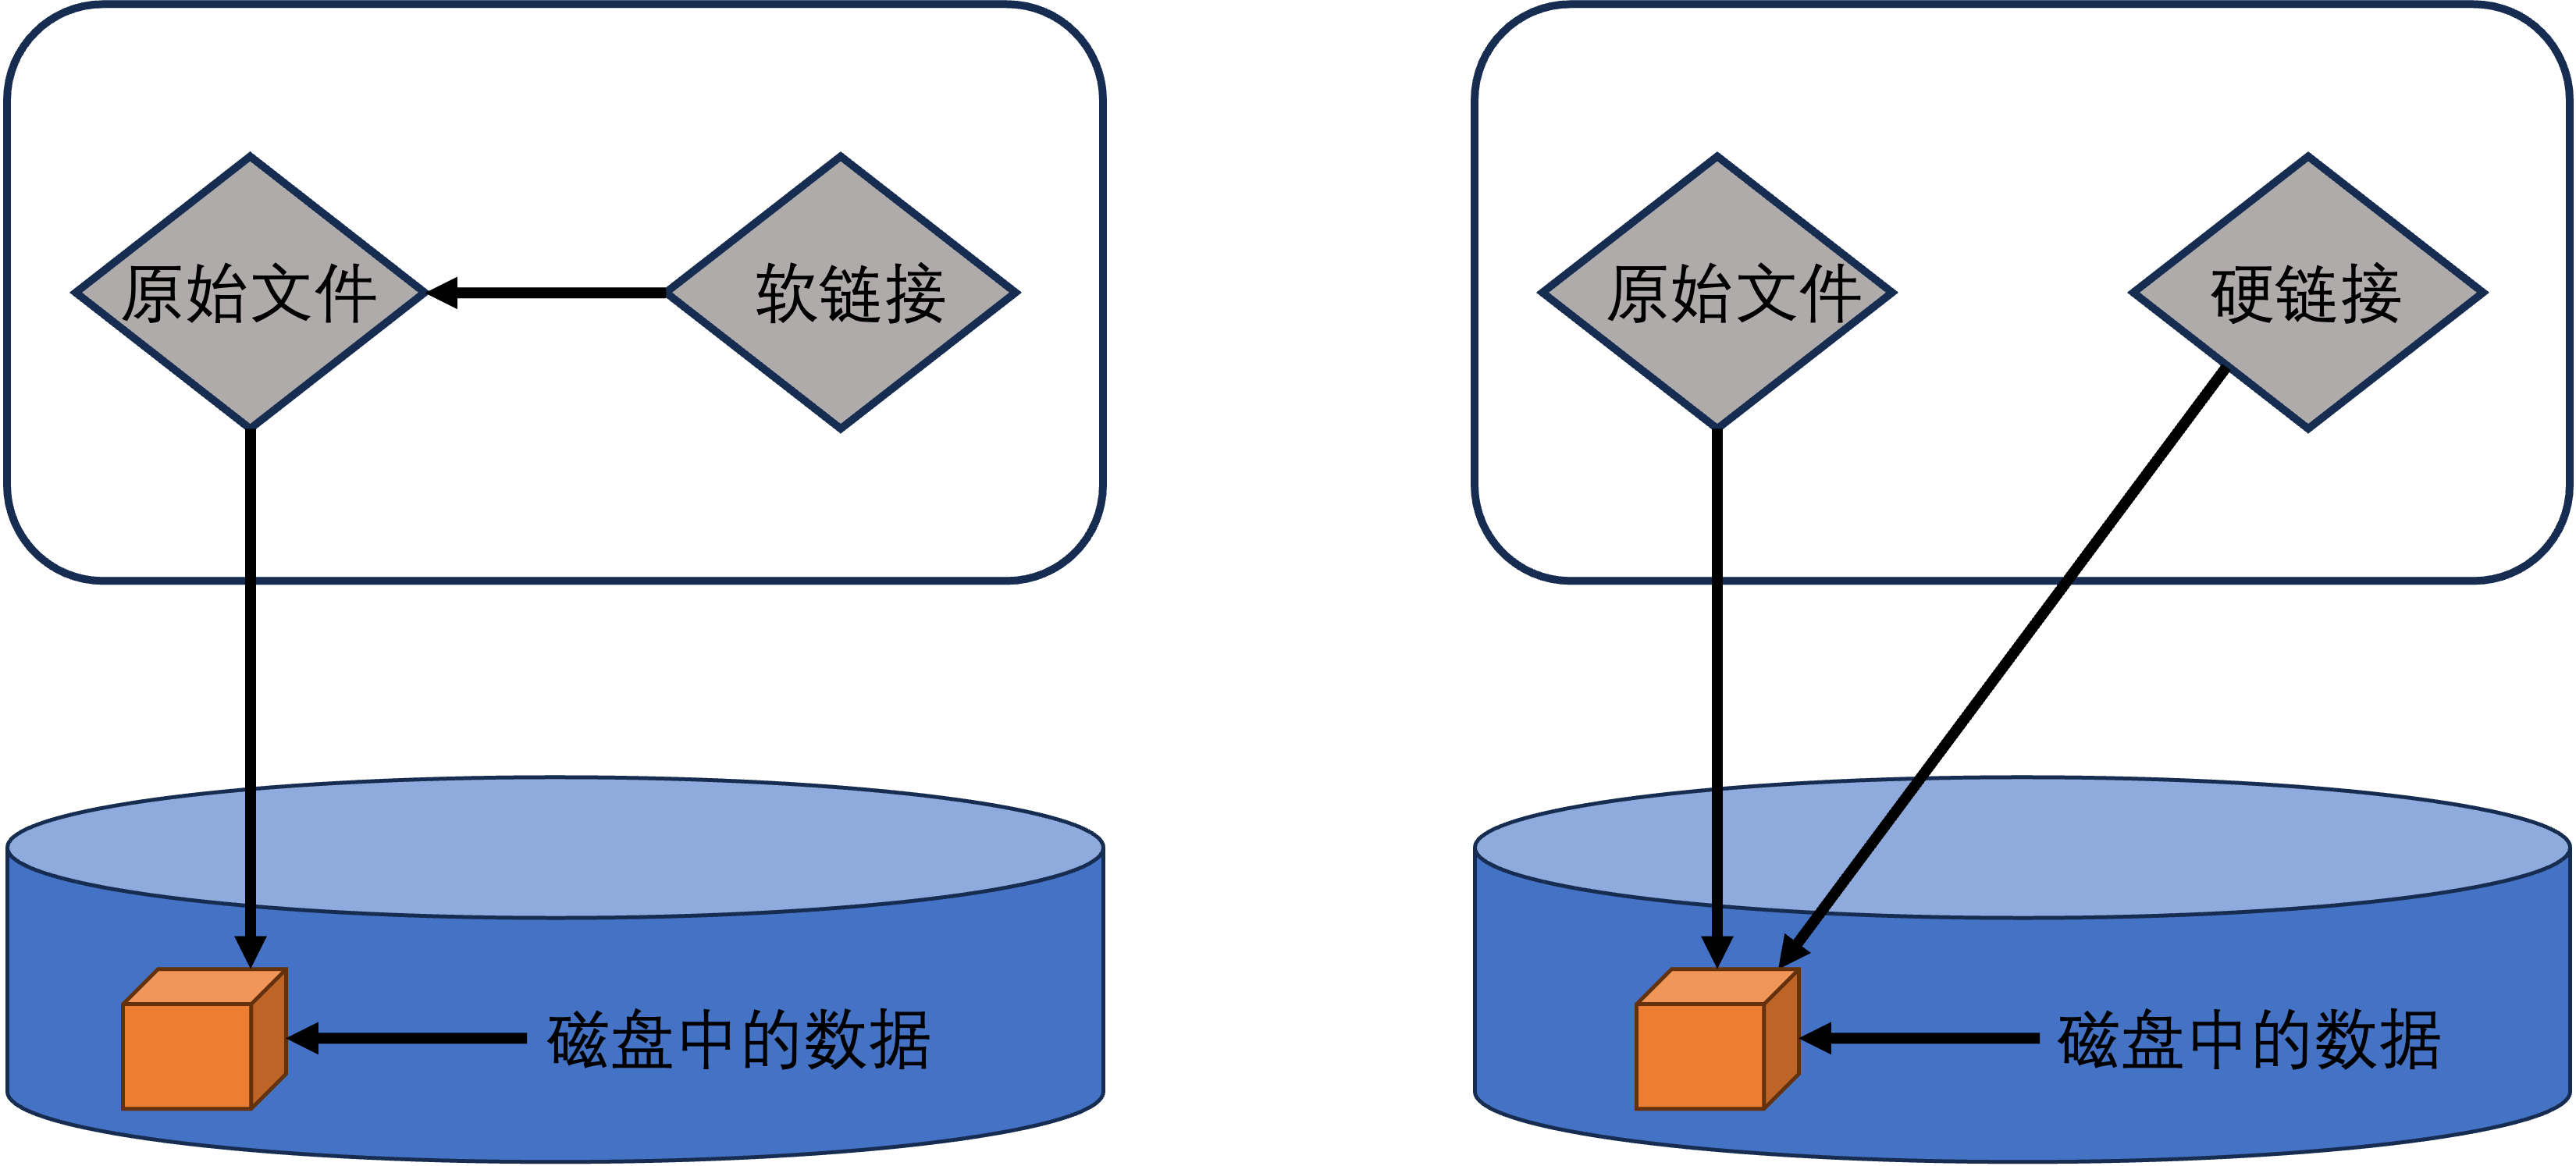
\includegraphics[width=\textwidth]{figures/07-09-软连接与硬连接示意图.png}
    \caption{
        软链接与硬链接示意图
    }
    \label{fig:link}
\end{figure}

\subsection{管道机制}

\chapter{理解文件系统}
\section{文件共享与PIPE}
\subsection{管道机制}
管道是一种最基本的进程间通信机制,作用于有血缘关系的进程之间,完成数据传递。其本质是一个伪文件,也就是一个小的内核缓冲区,作为一对文件描述符暴露给进程,一个用于读取,一个用于写入。将数据写入管道的一端使得该数据可用于从管道的另一端读取。

与管道相关的系统调用有pipe、write、read等,功能分别为创建、写入、读取管道。后两个系统调用已在其他章节详细解释,在这里着重介绍pipe系统调用。pipe系统调用的定义如下:
\begin{lstlisting}[language=rust]
    sys_pipe2(pipefd: usize, flags: u32) -> isize
\end{lstlisting}

pipeline ()创建一个管道,一个可用于进程间通信的单向数据通道。数组pipefd用于返回两个引用管道末端的文件描述符。pipefd[0]指的是管道的读取端。pipefd[1]指的是管道的写端。写入管道写入端的数据由内核缓冲,直到从管道读取端读取。

flags可以包含如下标志位:

O_CLOEXEC。设置两个读写文件描述符的close-on-exec标志。正常情况下,当一个进程执行一个新的程序时,新程序会继承其父进程的文件描述符。文件描述符是用于访问文件、套接字和其他I/O资源的抽象。O_CLOEXEC标志则用于指定文件描述符在执行新程序时是否应该被关闭。当设置过此标志后,执行一个新程序时,该文件描述符会被自动关闭。也就是说,新程序将不再继承父进程中的这个文件描述符。
              
O_DIRECT。创建一个以“分组”模式进行I/O的管道。对管道的每次write都被视为一个单独的分组,而从管道读取数据时,read系统调用将一次读取一个分组。需要注意的点有:大于PIPE_BUF字节的写操作将被拆分成多个分组。如果read指定的缓冲区大小小于下一个分组的大小,则将读取请求的字节数,并丢弃分组中的多余字节。指定缓冲区大小为PIPE_BUF足以读取可能的最大分组。不支持零长度的分组,read指定缓冲区大小为零的操作是无操作的,并返回0。

O_NONBLOCK。在新文件描述符所引用的打开文件描述符上设置O_NONBLOCK文件状态标志,指示文件描述符应该以非阻塞模式打开。在非阻塞模式下,文件描述符的 I/O 操作不会阻塞(即不会导致调用进程挂起等待),而是会立即返回,无论操作是否完成。这种模式在需要异步操作或需要避免长时间阻塞的场景下非常有用。

当前,在NPUCore中,只支持O_CLOEXEC标志位。

在内核中,pipe的数据结构本质上是一个环形队列,数据从写端流入管道,从读端流出,这样就实现了进程间通信。对应NPUCore的代码如下。队列被初始化为空( head=tail=0),且没有写端的引⽤计数。
\begin{lstlisting}[language=rust]
    impl PipeRingBuffer {
    fn new() -> Self {
        // let mut vec = Vec::<u8>::with_capacity(RING_DEFAULT_BUFFER_SIZE);
        // unsafe {
        //     vec.set_len(RING_DEFAULT_BUFFER_SIZE);
        // }
        Self {
            arr: Box::new([0u8; RING_DEFAULT_BUFFER_SIZE]),
            head: 0,
            tail: 0,
            status: RingBufferStatus::EMPTY,
            write_end: None,
            read_end: None,
        }
    }
}
\end{lstlisting}

初始化这个队列之后,实例化两个 Pipe 两端,并分别定义为写端与读端,也就是设置其对应的标志位:
\begin{lstlisting}[language=rust]
    impl Pipe {
    pub fn read_end_with_buffer(buffer: Arc<Mutex<PipeRingBuffer>>) -> Self {
        Self {
            readable: true,
            writable: false,
            buffer,
        }
    }
    pub fn write_end_with_buffer(buffer: Arc<Mutex<PipeRingBuffer>>) -> Self {
        Self {
            readable: false,
            writable: true,
            buffer,
        }
    }
}
\end{lstlisting}

上述代码已经完成了sys_pipe2系统调用的主体过程。

\begin{figure}[htb]
    \centering
    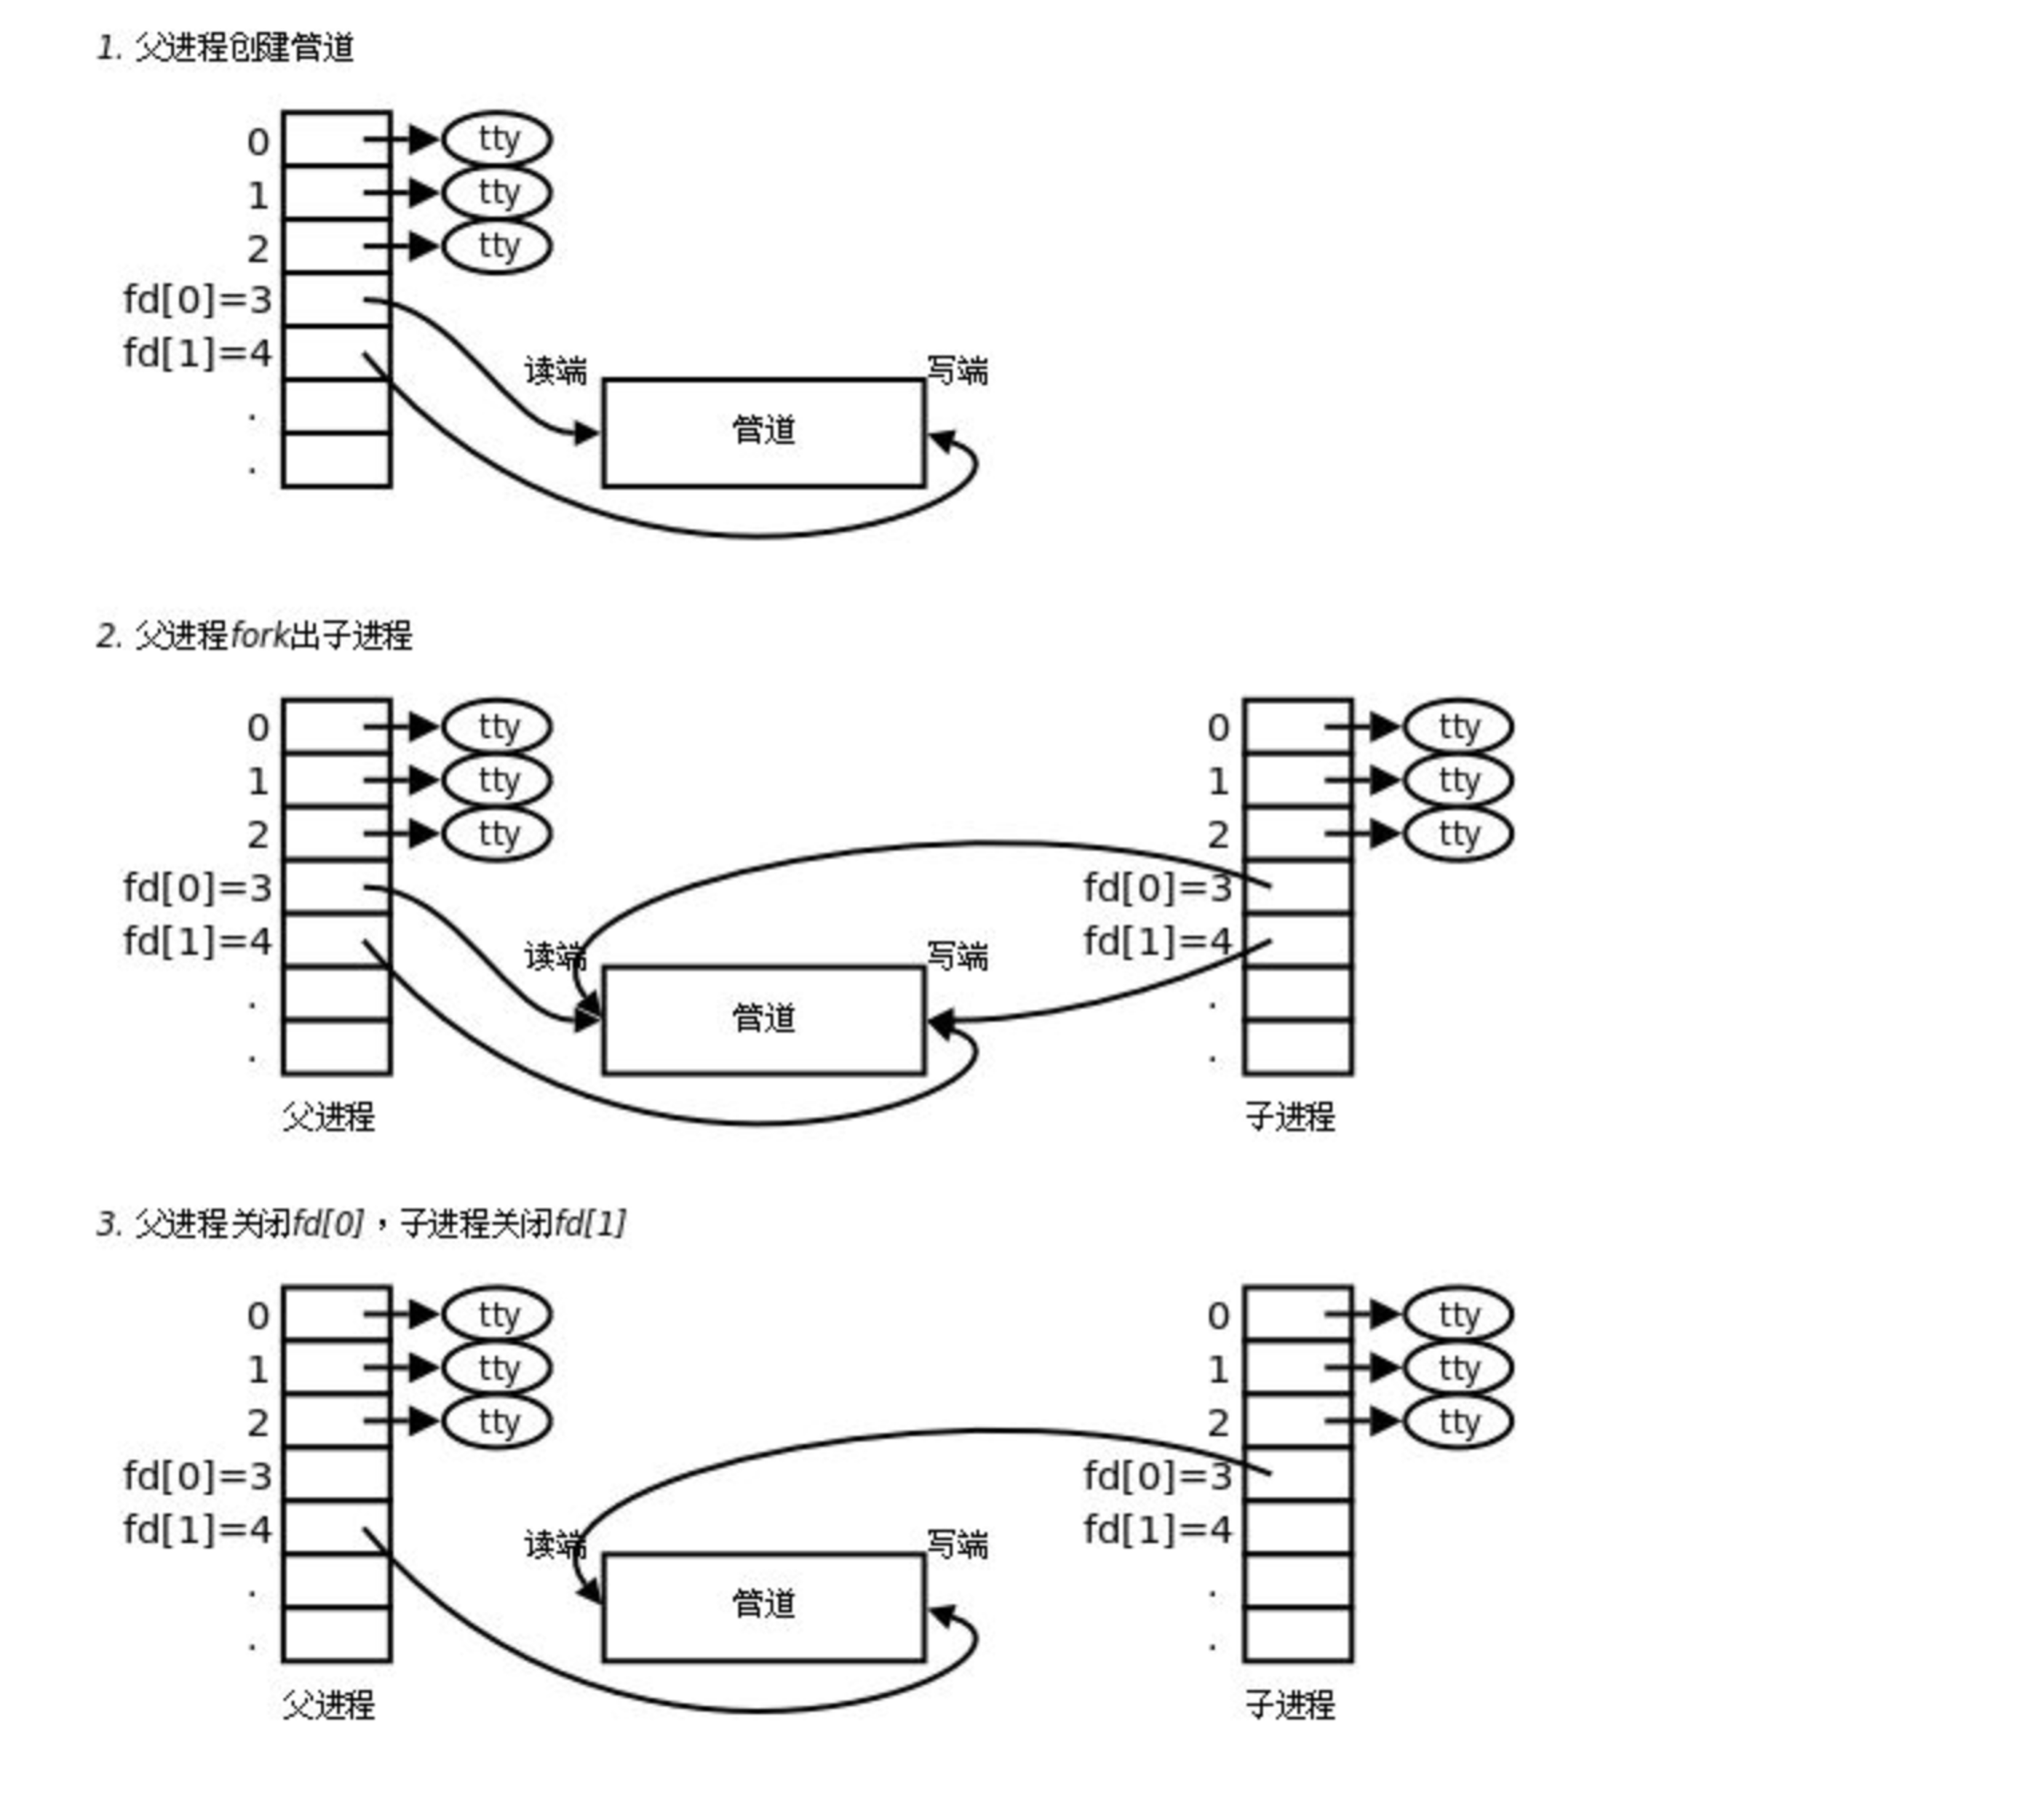
\includegraphics[width=\textwidth]{figures/07-09-管道操作示意图.png}
    \caption{
        管道操作示意图
    }
    \label{fig:pipe}
\end{figure}

下面介绍pipe的使用过程。一般情况下,管道创建成功以后,创建该管道的进程(父进程)同时掌握着管道的读端和写端。要实现父子进程间通信,通常可以采用如\ref{fig:pipe}所示的步骤:

1. 父进程调用pipe系统调用创建管道,得到两个文件描述符pipefd[0]、pipefd[1]指向管道的读端和写端。

2. 父进程调用fork创建子进程,那么子进程也有两个文件描述符指向同一管道。

3. 父进程关闭管道读端,子进程关闭管道写端。父进程可以向管道中写入数据,子进程将管道中的数据读出。

使用管道时,存在以下4种特殊情况(假设都是阻塞I/O操作,没有设置O_NONBLOCK标志):

1. 如果所有指向管道写端的文件描述符都关闭了(管道写端引用计数为0),而仍然有进程从管道的读端读数据,那么管道中剩余的数据都被读取后,再次read会返回0,就像读到文件末尾一样。

2. 如果有指向管道写端的文件描述符没关闭(管道写端引用计数大于0),而持有管道写端的进程也没有向管道中写数据,这时有进程从管道读端读数据,那么管道中剩余的数据都被读取后,再次read会阻塞,直到管道中有数据可读了才读取数据并返回。

3. 如果所有指向管道读端的文件描述符都关闭了(管道读端引用计数为0),这时有进程向管道的写端write,那么该进程会收到信号SIGPIPE,通常会导致进程异常终止。当然也可以对SIGPIPE信号实施捕捉,不终止进程。具体方法信号章节详细介绍。

4. 如果有指向管道读端的文件描述符没关闭(管道读端引用计数大于0),而持有管道读端的进程也没有从管道中读数据,这时有进程向管道写端写数据,那么在管道被写满时再次write会阻塞,直到管道中有空位置了才写入数据并返回。


最后介绍pipe的关闭过程。由于系统调⽤ sys_pipe 为参数 pipe 写⼊了写端和读端两个指向进程控制块的⽂件描述符表的相关位置,通过系统调⽤ sys_close 可以⽤关闭⽂件的相同的⽅式关闭管道的⼆端。sys_close 将⽂件描述符标记为空,会使得对应的 Arc 引⽤被销毁。写端和读端都被关闭后,buffer的引⽤对象,即管道⾃⾝的引⽤计数减少到0,导致管道⾃⾝被销毁,管道也得以关闭。




\chapter{嵌入式硬件平台简介及内核运行}
\section{基于嵌入式硬件的操作系统开发流程}

\subsection{串口简介}

\subsubsection{什么是串口}

串口是串行接口(Serial Port)的简称,是一种常用的计算机接口。由于连线少、通信控制简单而得到广泛的使用。串口有几种标准,常见的一种称为 RS232 接口的标准是在1970年由美国电子工业协会(EIA)和几家计算机厂商共同制定的。RS232标准应用广泛,其全称是“数据终端设备(DTE)和数据通讯设备(DCE)串行二进制数据交换接口”,该标准定义了串口的电气接口特性和各种信号电平等。


标准串口协议支持的最高数据传输率是115Kbps。一些改进的串口控制器支持更高甚至460Kbps的数据传输率,如增强型串口ESP(Enhanced Serial Port)和超级增强型串口Super ESP。


RS232 串口使用D型数据接口,最初有9针和25针两种连接方式。随着计算机技术的不断进步,25针的串口连接方式已经被淘汰,目前所有的RS232串口都使用9针连接方式。

\subsubsection{串口工作原理}

串口通过直接连接在两台设备之间的线发送和接收数据,两台设备通信最少需要三根线(发送数据、接收数据和接地)才可以通信。以最常见的RS232串口为例,通信距离较近时(<12m),可以用电缆线直接连接标准RS232端口。如果传输距离远,可以通过调制解调器(MODEM)传输。因为串口设备工作频率低且容易受到干扰,远距离传输会造成数据丢失。

\begin{table}[!ht]
	\centering
	\begin{tabular}{|c|c|c|}
		\hline
		\textbf{针号} & \textbf{功能说明} & \textbf{缩写} \\
		\hline
		1 & 数据载波检测 & DCD  \\
		2 & 接收数据 & RXD  \\
		3 & 发送数据 & TXD \\
		4 & 数据终端准备 & DTR \\
		5 & 信号地 & GND \\
		6 & 数据设备准备好 & DSR \\
		7 & 请求发送 & RTS \\
		8 & 清除发送 & CTS \\
		9 & 振铃指示 & BELL \\
		\hline
	\end{tabular}
	\caption{DB9接口的RS232 串口数据线定义}
	\label{DB9接口的RS232 串口数据线定义}
\end{table}

表 \ref{DB9接口的RS232 串口数据线定义}是常见的9针接口串口各条线定义,RS232标准的串口不仅提供了数据发送和接收的功能,同时可以进行数据流控制。对于普通应用来说,连接好两个数据线和地线就可以通信。

\subsubsection{Windows系统下的串口工具}

MobaXterm 又名 MobaXVT,是一款增强型终端、X 服务器和 Unix 命令集(GNU/ Cygwin)工具箱。可以开启多个终端视窗,以最新的 X 服务器为基础的 X.Org,可以轻松地来试用 Unix/Linux 上的 GNU Unix 命令。这样一来,我们可以不用安装虚拟机来试用虚拟环境,然后只要通过 MobaXterm 就可以使用大多数的 linux 命令。MobaXterm 还有很强的扩展能力,可以集成插件来运行 Emacs、Fontforge、Gcc, G++ and development tools、MPlayer、Perl、Curl、Corkscrew、 Tcl / Tk / Expect、 Screen、 Png2Ico 、 NEdit  Midnight Commander 等程序。


MobaXterm的下载较为简单,进入官网直接下载即可。需要注意的是MobaXterm 分免费家庭版和收费专业版:
\begin{itemize}
	\item 家庭版(Home):家庭版又分便捷版和安装版。便捷版不需要安装,下载压缩包后解压即可使用。安装版则需一步步安装后才能使用。
	\item 专业版(Professional):专业版会在 Session数、SSH tunnels 数和其他一些定制化配置进行限制。
\end{itemize}

MobaXterm的界面结构为:
\begin{itemize}
	\item 主页:打开MobaXterm后,绝大部分内容会被主页占据,主页有快捷按钮“start local terminal”以及最近的Session记录,可以方便打开终端,进行命令行操作。
	\item 菜单栏:MobaXterm的菜单栏如下,分为menu bar和buttons bar两行。用户可通过menu bar设置MobaXterm。buttons bar则为用户提供了一系列功能,如用户可通过Session启动远程会话,选择创建 SSH、Telnet、Rlogin、RDP、VNC、XDMCP、FTP、SFTP 或串行会话。开始的每个会话都会自动保存并显示在左侧边栏中。
	\item 侧边栏:侧边栏分为三个视图,分别为Sessions,Tools,Macros。Sessions负责管理使用过的Session配置,可以在任意Session选项上右击进行编辑。Tools分为四部分Terminal games、System、Office、NetWork的工具集合。使用非常的方便。Macros可以录制操作过程,下次使用时直接回放即可。
\end{itemize}

\begin{figure}[h]
	\centering
	\includegraphics[width=0.6\textwidth]{figures/08-01-mobaXterm界面.png}
	\caption{mobaXterm界面}
	\label{mobaXterm界面}
\end{figure}


MobaXterm是一款功能强大的综合性工具,支持SSH、RDP、FTP、Serial等多种通信协议。在本节中,我们将重点介绍其支持的Serial协议功能。MobaXterm可用作串口终端,与串口调试助手等工具相比,它提供了更强大的功能。在使用串口调试助手等工具时,虽然可以用于打印调试信息,但无法实现终端使用,即不能输入命令。


在MobaXterm中,通过点击"Session",选择"Serial",打开串口设置窗口。首先,选择要配置的串口号,并使用串口线将开发板连接到计算机上。然后,设置波特率,MobaXterm软件能够自动识别串口,用户只需从下拉菜单中选择相应的波特率。此外,还需进行其他串口功能的设置。点击"Advanced Serial settings"选项卡,可配置串口的其他功能,包括串口号、数据位、停止位、奇偶校验和硬件流控等。若需配置与终端相关的功能,则可点击"Terminal settings",进行相关设置,如终端字体以及字体大小等。完成设置后,点击窗口下方的"OK"按钮即可。

\subsubsection{Linux系统下的串口工具}

串口是嵌入式开发使用最多的通信方式。Linux系统提供了一个串口工具minicom,可以完成复杂的串口通信工作。若将minicom移植到板卡上,我们就可以借助minicom对串口进行读写操作。


本节介绍 minicom的使用。首先是安装 minicom,在 Ubuntu Linux 系统 shell 下输入“sudo apt-get install minicom”,按回车键后即可安装minicom 软件。软件安装好后,第一次使用之前需要配置minicom。

\begin{enumerate}
	\item 在shell中输入 sudo minicom-s,出现 minicom配置界面,下图 \ref{minicom配置界面}所示。minicom配置菜单在屏幕中央,每个菜单项都包括了一组配置。
	\begin{figure}[h]
		\centering
		\includegraphics[width=0.4\textwidth]{figures/08-01-minicom配置界面.png}
		\caption{minicom配置界面}
		\label{minicom配置界面}
	\end{figure}

	\item 用光标键移动高亮条到 Serial Port setup菜单项,按回车键后进入串口参数配置界面,如下图 \ref{minicom配置端口界面}所示。串口配置界面列出了串口的配置,每个配置前都有一个英文字母,代表进入配置项的快捷键。首先配置端口,输入小写字母a,光标移动到了/dev/tty8字符串最后,并且进入
	到编辑模式。以笔者机器为例,修改为/dev/tty0,代表连接到系统的第一个串口。
	\begin{figure}[h]
		\centering
		\includegraphics[width=0.6\textwidth]{figures/08-01-minicom配置端口界面.png}
		\caption{minicom配置端口界面}
		\label{minicom配置端口界面}
	\end{figure}

	\item 配置好串口设备后按回车键,保存参数并且回到提示界面。输入小写字母e,进入串口参数配置界面,如下图 \ref{minicom配置串口参数}所示。串口参数界面可以配置串口波特率、数据位、停止位等信息。一般只需要配置波特率,如在笔者机器上需要配置波特率是38400,输入小写字母d,屏幕上方current字符串后的波特率改变为38400。
	\begin{figure}[h]
		\centering
		\includegraphics[width=0.6\textwidth]{figures/08-01-minicom配置串口参数.png}
		\caption{minicom配置串口参数}
		\label{minicom配置串口参数}
	\end{figure}

	\item 设置好波特率后按回车键,保存退出,回到串口配置界面,如下图 \ref{minicom配置端口结束}所示。串口被设置为tty0,波特率是38400,其他配置使用默认设置。如果保存配置,直接按回车键退出。选择Save setup as dfl选项后按回车键,配置信息被保存为默认配置文件,下次启动的时候会自动加载。保存默认配置后,选择Exit选项后按回车键,退出配置界面,minicom自动进入终端界面。在终端界面会自动连接到串口,如果串口没有连接任何设备,屏幕右下角的状态提示为Offline。
	\begin{figure}[h]
		\centering
		\includegraphics[width=0.6\textwidth]{figures/08-01-minicom配置端口结束.png}
		\caption{minicom配置端口结束}
		\label{minicom配置端口结束}
	\end{figure}

	\item 退出 minicom,使用Ctrl+a键,然后输入字母z,出现minicom的命令菜单,如下图 \ref{minicom命令界面}所示。
	\begin{figure}[h]
		\centering
		\includegraphics[width=0.6\textwidth]{figures/08-01-minicom命令界面.png}
		\caption{minicom命令界面}
		\label{minicom命令界面}
	\end{figure}
\end{enumerate}



Minicom 提供了丰富的功能,是 Linux 中串口通信和远程管理的重要工具:

\begin{itemize}
	\item 调试和配置串口设备: Minicom 可以连接和调试各种串口设备,如调制解调器、路由器、交换机等。用户可以通过 Minicom 查看设备的输出信息,发送指令进行配置和调试。

	\item 远程终端连接: Minicom 可以作为一个终端仿真器,用于远程连接到其他计算机或设备。通过串口连接,用户可以在本地计算机上操作远程设备,进行远程管理和维护。

	\item 数据传输和文件传输: Minicom 支持通过串口进行数据传输,可用于传输文件、备份数据等。用户可以通过 Minicom 将文件发送到远程设备或从远程设备接收文件。

	\item 系统调试和故障排查: Minicom 可用于调试和排查系统故障。通过串口连接到系统控制台,用户可以查看系统的启动信息、错误日志等,帮助定位和解决问题。

	\item 嵌入式开发和调试: 对于嵌入式系统开发者来说,Minicom 是一个重要的工具。它可用于与嵌入式设备进行通信,进行程序下载、调试和测试。
\end{itemize}
\section{基于RISC-V64的NPUcore内核运行}
\section{基于LoongArch的NPUcore内核运行}

\chapter{编写面向POSIX标准的系统调用}
\section{POSIX标准简介}
\section{BusyBox简介}
\subsection{简单介绍}

\begin{figure}[htb]
	\centering
	\includegraphics[width=\textwidth]{figures/09-02-Busybox源码目录结构.png}
	\caption{
		Busybox源码目录结构
	}
	\label{fig:user virtual process}
\end{figure}

BusyBox是一个针对嵌入式系统的轻量级工具集合,旨在通过整合常用的
Linux命令和服务程序,将它们合并为一个单一的可执行文件。这个项目
最初于1996年诞生,当时嵌入式系统并不像今天这般普及。BusyBox的
最初目的是为软盘系统设计的,因为在那个时候,可移动存储介质的容
量十分有限,软盘是主要的存储媒介之一。

BusyBox的设计理念非常巧妙。相较于单独存放每个命令所需的存储空间
,BusyBox通过将不同命令的共享部分整合到一起,极大地减小了可执行
文件的体积。举例来说,诸如grep和find这样的命令,尽管功能有所差
异,但它们都需要从文件系统中搜索文件,BusyBox将这部分代码进行
共享,从而节省了空间。

BusyBox的核心特点在于其高度紧凑的特性。它可以包含最基本的系统
命令,例如文件列表显示命令ls和文件内容查看命令cat,同时也能整
合更复杂的程序,如文本搜索命令grep和文件查找命令find,甚至还
能将HTTP服务器整合进同一个软件包中。

对于嵌入式系统来说,存储空间十分宝贵,而BusyBox的存在则为这些
系统提供了解决方案。通常情况下,BusyBox的可执行文件大小仅约1MB
左右,相比于分散存放各个命令所需的存储空间,这是一个相当节省空间
的选择。用户可以通过建立链接的方式,与传统的命令一样使用BusyBox
,只不过它将多个功能整合到一个文件中,从而在嵌入式系统中占用更少
的存储空间。

Busybox源码目录结构图如上,方便以后对Busybox做裁剪的时候参考。

\subsection{工作原理}
BusyBox利用了shell传递给C语言main()函数的参数,回想一下C语言
main()函数的定义:int main(int argc,char *argv[])

在main()函数的定义中argc是传递进来的参数个数,argv是一个字符串
数组,数据的每一项都是一个参数内容。其中,argv[0]是从命令行调用
的程序名。下面是一个简单的程序,使用argv[0]确定调用来自哪个程序
。

\begin{lstlisting}[language=Rust]
	//test.c
	#include <stdio.h>
	/*定义主函数*/
	int main(int argc,char *argv[])
	int i;
	for(i=0;i<argc ;i++){
		//for循环语句
		printf("argv[8d]=8s\n",i,argv[i]);//打印程序参数内容
	 }
	return 0;
    }
\end{lstlisting}

调用这个程序会显示所调用的第一个参数是该程序的名字。可以对这个可执行程序重新进行命名,此时再调用就会得到该程序的新名字。另外,可以创建一个到可执行程序的符号链接,在执行这个符号链接时,就可以看到这个符号链接的名字。

\begin{lstlisting}[language=Rust]
	$  gcc -Wall -o test test.c
	$  ./test argl arg2
	argv[0]=./test
	argv[1]=arg1
	argv[2]=arg2

	$  mv test newtest
	$  ./newtest argl
	argv[0]=./newtest
	argv[1]=arg1

	$  ln -s newtest linktest
	$  ./linktest arg
	argv[0]=./linktest
	argv[1]=arg
	\end{lstlisting}

BusyBox使用符号链接屏蔽了程序调用细节。从用户的角度看,使用BusyBox与使用传统的命令效果是相同的。BusyBox为其包含的每个系统程序都建立了类似的符号链接。当用户使用符号链接调用BusyBox的时候,BusyBox通过argv[0]参数调用对应的功能函数。

\subsection{使用方法}
\subsubsection{BusyBox初始化}
Linux内核的初始化代码里有如下几个语句:
\begin{lstlisting}[language=Rust]
	if(execute_command)
	execve(execute_command,argv_init,envp_init);
	execve("/sbin/init",argv_init,envp_init);
\end{lstlisting}

execute\_command是内核启动参数。一般情况下配置启动命令行init=/linuxrc参数,内核会得到execute\_command=/linuxrc参数。当读取到启动参数的时候,内核会执行/linuxrc文件。通常情况下,/linuxrc是一个启动脚本,大致内容如下:
\begin{lstlisting}[language=Rust]
	#!/bin/sh
	exec /sbin/init
\end{lstlisting}

很简单的两句,指定了执行/sbin/init程序。在嵌入式系统上,安装BusyBox需要指定/sbin/init作为BusyBox可执行程序的一个软链接。这样,Linux内核到这里会执行BusyBox的代码。

BusyBox的入口在applets/busybox.c中,主要代码如下:
\begin{lstlisting}[language=Rust]
	int main(int argc,char **argv)
	const char *s;
	bb_applet_name =argv[0];
	if(bb_applet_name[0]=='-')bb_applet_name++;
	for(s~=bb_applet_name;*s !=‘Toi;)
	{
		if(*s++=='/')
		bb_applet_name =s;
		#ifdef CONFIG_LOCALE_SUPPORT
		#ifdef CONFIG_INIT
		if(getpid()!=1)/*Do not set locale for 'init'*/
		#endif
		{setlocale(LC_ALL,"");}
		#endif
		run_applet_by_name(bb_applet_name,argc,argv);
		bb_error_msg_and_die("applet not found");
		bb_applet_name =argv[0]
\end{lstlisting}

在main()函数中使用run\_applet\_by\_name()找到对应的代码运行。主要代码如下:
\begin{lstlisting}[language=Rust]
	if((applet_using =find_applet_by_name(name))!=NULL)
	{
		bb_applet_name =applet_using->name;
		exit(( * (applet_using->main))(argc,argv));
		struct BB_applet * find_applet_by_name(const char * name){
			return bsearch(name,applets,NUM_APPLETS,sizeof(struct BB_applet),applet_name_compare);
\end{lstlisting}

从run\_applet\_by\_name()代码看出,BusyBox从applets结构查找name参数对应的命令功能函数。applets结构定义如下:
\begin{lstlisting}[language=Rust]
	const struct BB_applet applets[]=(
	#define APPLET(a,b,c,d){#a,b,c,d},
	#define APPLET_NOUSAGE(a,b,c,d){a,b,c,d},#define APPLET_ODDNAME(a,b,c,d,e){a,b,c,d},
	#ifdef CONFIG_TEST
	APPLET_NOUSAGE("[",test_main,_BB_DIR_USR_BIN,_BB_SUID_NEVER)#endif
	#ifdef CONFIG_ADDGROUP
	APPLET(adagroup,addgroup_main,_BB_DIR_BIN,_BB_SUID_NEVER)#endif#ifdef CONFIG_ADDUSER
	APPLET(adduser,adduser_main,_BB_DIR_BIN,_BB_SUID_NEVER)#endif
\end{lstlisting}

由此看出,BusyBox添加命令只需要向applets结构添加相应的项即可。本节关心与启动有关的init项。

\begin{lstlisting}[language=Rust]
	#ifdef CONFIG_INITAPPLET(init,init_main,_BB_DIR_SBIN,_BB_SUID_NEVER)
	#endif
\end{lstlisting}

init项定义的主函数入口是init\_main(),说明系统启动的时候会执行该函数。函数定义在init/init.c文件中。init\_main()函数内容比较多,这里不一一列出。其中比较重要的是init\_main()函数调用了3个函数:

parse inittab(),

run\_actions(SYSINIT),

run\_actions(ASKFIRST);

parse\_inittab()函数会解析/etc/inittab文件,然后执行该文件。之后该函数会注册一些函数,处理/etc/init.d/rcS这个脚本,通过run\_actions()函数处理脚本的内容。
\begin{lstlisting}[language=Rust]
	static void run_actions(int action)
	{
		struct init_action *a,*tmp;
		for (a =init_action_list;a;a =tmp)
		{
		tmp =a->next;
		if(a->action ==action)
		//判断输入的动作是否与列表中的动作相符
		{
		if(a->action&(SYSINIT I WAIT I CTRLALTDEL I SHUTDOWN I RESTART))
		//检查动作范围
		{
		waitfor(a);
		//等待特定动作
		delete_init_action(a);//删除初始化动作
	    }
	else if(a->action &ONCE)//运行一次的动作
	    {
		run(a);
		//运行动作
		delete_init_action(a);//删除初始化动作
	    }
	else if(a->action 6(RESPAWN I ASKFIRST))
	//检查是否后台运行
	{
		if(a->pid ==0) a->pid =run(a);  //后台执行动作
	    }
      }
     }
    }
\end{lstlisting}

这样,在执行/sbin/init程序的时候会执行busybox并且找到正确的入口执行。依此类推,把系统常用的命令都建立到busybox的软链接上,BusyBox基本安装完毕了。最后还需要更新一下inittab文件以符合BusyBox需要。以下给出一个inittab文件的范例。
\begin{lstlisting}[language=Rust]
	#/etc/inittab init(8) configuration for BusyBox
	#
	#Copyright (C) 1999-2004 by Erik Andersen <andersenecodepoet.org>
	#Note,BusyBox init doesn't support runlevels.The runlevels field is
	#completely ignored by BusyBox init.If you want runlevels,use sysvinit.
	#
	#
	#Format for each entry:<id>:<runlevels>:<action>:<process>
	//表项格式
	#
	#<id>:WARNING:This field has a non-traditional meaning for BusyBox init!
	#
	#The id field is used by BusyBox init to specify the controlling tty for
	#the specified process to run on.The contents of this field are
	#appended to "/dev/" and used as-is.There is no need for this field to
	#be unique,although if it isn't you may have strange results.If this
	#field is left blank,it is completely ignored.Also 	note that if
	#BusyBox detects that a serial console is in use,then all entries
	#containing non-empty id fields will _not_be run.BusyBox init does
	#nothing with utmp.We don't need no stinkin'utmp.
	#
	#<runlevels>:The runlevels field is completely ignored.
	#
	#<action>:Valid actions include:sysinit,respawn,askfirst,wait,once,#restart,ctrlaltdel,and shutdown.
	//执行动作的格式
	#
	#   Note:askfirst acts just like respawn,but before running the
	specified
	#   process it displays the line "Please press Enter to activate this
	#   console."and then waits for the user to press enter before starting
	#   the specified process.
	#   Note : unrecognised actions (like initdefault)will cause init to emit
	#   an error message,and then go along with its business.
	#
	#<process>:Specifies the process to be executed and it's command line.
	//进程处理
	#
	#Note:BusyBox init works just fine without an inittab.If no inittab is
	#found,it has the following default behavior: 
	//BusyBox执行inittab文件,如果该文件不存在,执行下面的脚本
	#     ::sysinit:/etc/init.d/rcs
	#     ::askfirst:/bin/sh
	#     ::ctrlaltdel:/sbin/reboot
	#     ::shutdown:/sbin/swapoff -a
	#     ::shutdown:/bin/umount -a -r
	#     ::restart:/sbin/init
	# if it detects that /dev/console is _not_a serial console,it will also run:
	# //如果/dev/console设备不是串口设备,则执行下面的命令
	#     tty2::askfirst:/bin/sh
	#     tty3::askfirst:/bin/sh
	#     tty4::askfirst:/bin/sh
	#
	#Boot-time system configuration/initialization script.
	#This is run first except when booting in single-user mode.  //启动时运行的脚本
	#
	::sysinit:/etc/init.d/rcs

	# /bin/sh invocations on selected ttys
	#
	# Note below that we prefix the shell commands with a "-"to indicate to
	the
	# shell that it is supposed to be a login shell.Normally this is handled
	by
	#login,but since we are bypassing login in this case,BusyBox lets you do
	#this yourself...
	#
	#Start an "askfirst"shell on the console(whatever that may be)
	::askfirst:-/bin/sh
	#Start an "askfirst"shell on /dev/tty2-4
	tty2::askfirst:-/bin/sh
	tty3::askfirst:-/bin/sh
	tty4::askfirst:-/bin/sh
	#/sbin/getty invocations for selected ttys
	tty4::respawn:/sbin/getty 38400 tty5
	tty5::respawn:/sbin/getty 38400 tty6
	#Example of how to put a getty on a serial line(for a terminal)//建立串口控制台的例子
	#::respawn:/sbin/getty -L ttys09600 vt100
	#::respawn:/sbin/getty -L ttys19600 vt100
	#
	#Example how to put a getty on a modem line. //如何建立Modem连接的例子#::respawn:/sbin/getty 57600 ttyS2
	#Stuff to do when restarting the init process //设置什么时候执行init程序
	::restart:/sbin/init
	#Stuff to do before rebooting  //设置重新启动之前做什么
	::ctrlaltdel:/sbin/reboot
	::shutdown:/bin/umount -a -r
	::shutdown:/sbin/swapoff -a
\end{lstlisting}

读者可以根据自己的需要修改范例文件。

这个函数可以判读rcS脚本中执行的类型,执行完rcS脚本后,系统可以进入shell界面。BusyBox有4种类型的shell,默认使用ash。执行完脚本后,BusyBox会启动脚本,进入命令行。

\subsubsection{目标板BusyBox安装}
了解了BusyBox的工作流程后,安装BusyBox就变得很简单了。主要的任务是设置好BusyBox与Linux内核的结合点。

可以通过两种手段设置BusyBox到开发板。一种方法是在PC上制作cramfs镜像。这种方法的好处是便于操作,但是需要注意的是,BusyBox的路径不能搞错;缺点是出错后修改比较麻烦,每次都需要烧写开发板的Flash。

如果开发板已经有系统,可以通过上传的方法。把可执行文件busybox上传到开发板Linux系统的/bin下,然后修改/sbin/init链接到busybox。

ln -s /bin/busybox /sbin/init

这样,在执行/sbin/init程序的时候会执行busybox并且找到正确的入口执行。依此类推,把系统常用的命令都建立到busybox的软链接上,BusyBox基本安装完毕了。最后还需要更新一下inittab文件以符合BusyBox需要。本书给出一个inittab文件的范例。

\begin{lstlisting}[language=Rust]
	#/etc/inittab init(8) configuration for BusyBox
	#
	#Copyright(C)1999-2004 by Erik Andersen <andersenecodepoet.org>
	#
	#
	#Note,BusyBox init doesn't support runlevels.The runlevels field is
	#completely ignored by BusyBox init.If you want runlevels,use sysvinit.
	#
	#
	#Format for each entry:<id>:<runlevels>:<action>:<process>//表项格式
	#
	#<id>:WARNING:This field has a non-traditional meaning for BusyBox init!
	#
	#The id field is used by BusyBox init to specify the controlling try for
	#the specified process to run on.The contents of this field are
	#appended to"/dev/"and used as-is.There is no need for this field to
	#be unique,although if it isn't you may have strange results.If this
	#field is left blank,it is completely ignored.Also note that if
	#BusyBox detects that a serial console is in use,then all entries
	#containing non-empty id fields will _not_be run.BusyBox init does
	#nothing with utmp.We don't need no stinkin'utmp.
	#
	#<runlevels>:The runlevels field is completely ignored.
	#
	#<action>:Valid actions include:sysinit,respawn,askfirst,wait,once,
	#restart,ctrlaltdel,and shutdown.
	//执行动作的格式
\end{lstlisting}

\subsection{常用的命令}
\subsubsection{安装和登录命令}
\textbf{reboot:}

作用:reboot命令的作用是重新启动计算机,它的使用权限是系统管理者。

格式:reboot [-n] [-w] [-d] [-f] [-i]

主要参数:

-n: 在重开机前不做将记忆体资料写回硬盘的动作。

-w: 并不会真的重开机,只是把记录写到/var/log/wtmp文件里。

-d: 不把记录写到/var/log/wtmp文件里(-n这个参数包含了-d)。

-i: 在重开机之前先把所有与网络相关的装置停止。

\textbf{mount:}

作用:mount命令的作用是加载文件系统,它的用权限是超级用户或/etc/fstab中允许的使用者。

格式:mount -a [-fv] [-t vfstype] [-n] [-rw][-F] device dir

主要参数:

-h:显示辅助信息。

-v:显示信息,通常和-f用来除错。

-a:将/etc/fstab中定义的所有文件系统挂上。

-F:这个命令通常和-a一起使用,它会为每一个mount的动作产生一个行程负责执行。在系统需要挂上大量NFS文件系统时可以加快加载的速度。

-f:通常用于除错。它会使mount不执行实际挂上的动作,而是模拟整个挂上的过程,通常会和-v一起使用。

-t vfstype:显示被加载文件系统的类型。

-n:一般而言,mount挂上后会在/etc/mtab中写入一笔资料,在系统中没有可写入文件系统的情况下,可以用这个选项取消这个动作。


\textbf{umount:}

作用:umount命令的作用是卸载一个文件系统,它的使用权限是超级用户或/etc/fstab中允许的使用者。

格式:unmount -a [-fFnrsvw] [-t vfstype] [-n] [-rw][-F] device dir

\textbf{使用说明:}
umount命令是mount命令的逆操作,它的参数和使用方法和mount命令是一样的。Linux挂装CD-ROM后,会锁定CD—ROM,这样就不能用CD-ROM面板上的Eject按钮弹出它。但是,当不再需要光盘时,如果已将/cdrom作为符号链接,请使用umount/cdrom来卸装它。仅当无用户正在使用光盘时,该命令才会成功。该命令包括了将带有当前工作目录当作该光盘中的目录的终端窗口。

\textbf{exit:}

作用:exit命令的作用是退出系统,它的使用权限是所有用户。

格式:exit

主要参数:

exit命令没有参数,运行后退出系统进入登录界面

\subsubsection{文件处理命令}

\textbf{mkdir:}

作用:mkdir命令的作用是建立名称为dirname的子目录,与MS DOS下的md命令类似,它的使用权限是所有用户。

格式:mkdir [options] 目录名

主要参数:

-m, --mode=模式:设定权限,与chmod类似。

-p, --parents:需要时创建上层目录;如果目录早已存在,则不当作错误。

-v, --verbose:每次创建新目录都显示信息。

--version:显示版本信息后离开。

\textbf{grep:}

作用:grep命令可以指定文件中搜索特定的内容,并将含有这些内容的行标准输出。grep全称是Global Regular ExpressionPrint,表示全局正则表达式版本,它的使用权限是所有用户。

格式:grep [options]

主要参数:

-c:只输出匹配行的计数。

-I:不区分大小写(只适用于单字符)。

-h:查询多文件时不显示文件名。

-l:查询多文件时只输出包含匹配字符的文件名。

-n:显示匹配行及行号。

-s:不显示不存在或无匹配文本的错误信息。

-v:显示不包含匹配文本的所有行。

\^:匹配正则表达式的开始行。

\$: 匹配正则表达式的结束行。

[ ]:单个字符,如[A]即A符合要求 。

[ - ]:范围,如[A-Z],即A、B、C一直到Z都符合要求 。

。:所有的单个字符。

* :有字符,长度可以为0。

\textbf{dd:}

作用:dd命令用来复制文件,并根据参数将数据转换和格式化。

格式:dd [options]

主要参数:

bs=字节:强迫 ibs=及obs=。

cbs=字节:每次转换指定的。

conv=关键字:根据以逗号分隔的关键字表示的方式来转换文件。

count=块数目:只复制指定的输入数据。

ibs=字节:每次读取指定的。

if=文件:读取内容,而非标准输入的数据。

obs=字节:每次写入指定的。

of=文件:将数据写入,而不在标准输出显示。

seek=块数目:先略过以obs为单位的指定的输出数据。

skip=块数目:先略过以ibs为单位的指定的输入数据。

\textbf{find:}

作用:find命令的作用是在目录中搜索文件,它的使用权限是所有用户。

格式:find [path][options][expression]

path指定目录路径,系统从这里开始沿着目录树向下查找文件。它是一个路径列表,相互用空格分离,如果不写path,那么默认为当前目录。

主要参数:

-depth:使用深度级别的查找过程方式,在某层指定目录中优先查找文件内容。

-maxdepth levels:
表示至多查找到开始目录的第level层子目录。level是一个非负数,如果level是0的话表示仅在当前目录中查找。

-mindepth levels:表示至少查找到开始目录的第level层子目录。

-mount:不在其它文件系统(如Msdos、Vfat等)的目录和文件中查找。

-version:打印版本。

—name:支持统配符*和?。

-atime n:搜索在过去n天读取过的文件。

-ctime n:搜索在过去n天修改过的文件。

-group grpoupname:搜索所有组为grpoupname的文件。

-user 用户名:搜索所有文件属主为用户名(ID或名称)的文件。

-size n:搜索文件大小是n个block的文件。

-print:输出搜索结果,并且打印。

\textbf{mv:}

作用:mv命令用来为文件或目录改名,或者将文件由一个目录移入另一个目录中,它的使用权限是所有用户。该命令如同DOS命令中的ren和move的组合。

格式:mv[options] 源文件或目录 目标文件或目录

主要参数:

-i:交互方式操作。如果mv操作将导致对已存在的目标文件的覆盖,此时系统询问是否重写,要求用户回答“y”或“n”,这样可以避免误覆盖文件。

-f:禁止交互操作。mv操作要覆盖某个已有的目标文件时不给任何指示,指定此参数后i参数将不再起作用。

\textbf{ls:}

作用:ls命令用于显示目录内容,类似DOS下的dir命令,它的使用权限是所有用户。

格式:ls [options][filename]

主要参数:

-a, --all:不隐藏任何以“.” 字符开始的项目。

-A, --almost-all:列出除了“ . ”及 “.. ”以外的任何项目。

--author:印出每个文件著作者。

-b, --escape:以八进制溢出序列表示不可打印的字符。

--block-size=大小:块以指定的字节为单位。

-B, --ignore-backups:不列出任何以 ~ 字符结束的项目。

-f:不进行排序,-aU参数生效,-lst参数失效。

-F, --classify:加上文件类型的指示符号 (*/=@| 其中一个)。

-g:like -l, but do not listowner。

-G, --no-group:inhibit display ofgroup information。

-i, --inode:列出每个文件的inode号。

-I, --ignore=样式:不印出任何符合Shell万用字符的项目。

-k:即--block-size=1K。

-l:使用较长格式列出信息。

-L, --dereference:当显示符号链接的文件信息时,显示符号链接所指示的对象,而并非符号链接本身的信息。

-m:所有项目以逗号分隔,并填满整行行宽。

-n, --numeric-uid-gid:类似-l,但列出UID及GID号。

-N, --literal:列出未经处理的项目名称,例如不特别处理控制字符。

-p, --file-type:加上文件类型的指示符号 (/=@| 其中一个)。

-Q, --quote-name:将项目名称括上双引号。

-r, --reverse:依相反次序排列。

-R, --recursive:同时列出所有子目录层。

-s, --size:以块大小为序。

\textbf{diff:}

作用:diff命令用于两个文件之间的比较,并指出两者的不同,它的使用权限是所有用户。

格式:diff [options] 源文件 目标文件

主要参数:

-a:将所有文件当作文本文件来处理。

-b:忽略空格造成的不同。

-B:忽略空行造成的不同。

-c:使用纲要输出格式。

-H:利用试探法加速对大文件的搜索。

-I:忽略大小写的变化。

-n --rcs:输出RCS格式。

\textbf{cmp:}

作用:cmp(“compare”的缩写)命令用来简要指出两个文件是否存在差异,它的使用权限是所有用户。

格式:cmp[options] 文件名

主要参数:

-l: 将字节以十进制的方式输出,并方便将两个文件中不同的以八进制的方式输出。

\textbf{cat:}

作用:cat(“concatenate”的缩写)命令用于连接并显示指定的一个和多个文件的有关信息,它的使用权限是所有用户。

格式:cat [options] 文件1 文件2……

主要参数:

-n:由第一行开始对所有输出的行数编号。

-b:和-n相似,只不过对于空白行不编号。

-s:当遇到有连续两行以上的空白行时,就代换为一行的空白行。

\textbf{ln:}

作用:ln命令用来在文件之间创建链接,它的使用权限是所有用户。

格式:ln [options] 源文件 [链接名]

主要参数:

-f:链结时先将源文件删除。

-d:允许系统管理者硬链结自己的目录。

-s:进行软链结(Symbolic Link)。

-b:将在链结时会被覆盖或删除的文件进行备份。

\subsubsection{系统管理命令}

\textbf{reboot:}

作用:df命令用来检查文件系统的磁盘空间占用情况,使用权限是所有用户。

格式:df [options]

主要参数:

-s:对每个Names参数只给出占用的数据块总数。

-a:递归地显示指定目录中各文件及子目录中各文件占用的数据块数。若既不指定-s,也不指定-a,则只显示Names中的每一个目录及其中的各子目录所占的磁盘块数。

-k:以1024字节为单位列出磁盘空间使用情况。

-x:跳过在不同文件系统上的目录不予统计。

-l:计算所有的文件大小,对硬链接文件则计算多次。

-i:显示inode信息而非块使用量。

-h:以容易理解的格式印出文件系统大小,例如136KB、254MB、21GB。

-P:使用POSIX输出格式。

-T:显示文件系统类型。

\textbf{top:}

作用:top命令用来显示执行中的程序进程,使用权限是所有用户。

格式:top [-] [d delay] [q] [c] [S] [n]

主要参数:

d:指定更新的间隔,以秒计算。

q:没有任何延迟的更新。如果使用者有超级用户,则top命令将会以最高的优先序执行。

c:显示进程完整的路径与名称。

S:累积模式,会将己完成或消失的子行程的CPU时间累积起来。

s:安全模式。

i:不显示任何闲置(Idle)或无用(Zombie)的行程。

n:显示更新的次数,完成后将会退出top。

\textbf{free:}

作用:free命令用来显示内存的使用情况,使用权限是所有用户。

格式:free [-b|-k|-m] [-o] [-s delay] [-t] [-V]

主要参数:

-b -k -m:分别以字节(KB、MB)为单位显示内存使用情况。

-s delay:显示每隔多少秒数来显示一次内存使用情况。

-t:显示内存总和列。

-o:不显示缓冲区调节列。

\textbf{kill:}

作用:kill命令用来中止一个进程。

格式:kill [ -s signal | -p ] [ -a ] pid ...

kill -l [ signal ]

主要参数:

-s:指定发送的信号。

-p:模拟发送信号。

-l:指定信号的名称列表。

pid:要中止进程的ID号。

Signal:表示信号。

\subsubsection{网络操作命令}

\textbf{ifconfig:}

作用:ifconfig用于查看和更改网络接口的地址和参数,包括IP地址、网络掩码、广播地址,使用权限是超级用户。

格式:ifconfig -interface [options] address

主要参数:

-interface:指定的网络接口名,如eth0和eth1。

up:激活指定的网络接口卡。

down:关闭指定的网络接口。

broadcast address:设置接口的广播地址。

pointopoint:启用点对点方式。

address:设置指定接口设备的IP地址。

netmask address:设置接口的子网掩码。

\textbf{ip:}

作用:ip是iproute2软件包里面的一个强大的网络配置工具,它能够替代一些传统的网络管理工具,例如ifconfig、route等,使用权限为超级用户。几乎所有的Linux发行版本都支持该命令。

格式:ip [OPTIONS] OBJECT [COMMAND [ARGUMENTS]]

主要参数:

-V,-Version 打印ip的版本并退出。

-s,-stats,-statistics 输出更为详尽的信息。如果这个选项出现两次或多次,则输出的信息将更为详尽。

-f,-family 这个选项后面接协议种类,包括inet、inet6或link,强调使用的协议种类。如果没有足够的信息告诉ip使用的协议种类,ip就会使用默认值inet或any。link比较特殊,它表示不涉及任何网络协议。

-4 是-family inet的简写。

-6 是-family inet6的简写。

-0 是-family link的简写。

-o,-oneline 对每行记录都使用单行输出,回行用字符代替。如果需要使用wc、grep等工具处理ip的输出,则会用到这个选项。

-r,-resolve 查询域名解析系统,用获得的主机名代替主机IP地址

\textbf{ping:}

作用:ping检测主机网络接口状态,使用权限是所有用户。

格式:ping [-dfnqrRv][-c][-i][-I][-l][-p][-s][-t] IP地址

主要参数:

-d:使用Socket的SO\_DEBUG功能。

-c:设置完成要求回应的次数。

-f:极限检测。

-i:指定收发信息的间隔秒数。

-I:网络界面使用指定的网络界面送出数据包。

-l:前置载入,设置在送出要求信息之前,先行发出的数据包。

-n:只输出数值。

-p:设置填满数据包的范本样式。

-q:不显示指令执行过程,开头和结尾的相关信息除外。

-r:忽略普通的Routing Table,直接将数据包送到远端主机上。

-R:记录路由过程。

-s:设置数据包的大小。

-t:设置存活数值TTL的大小。

-v:详细显示指令的执行过程。

\textbf{netstat:}

作用:检查整个Linux网络状态。

格式:netstat [-acCeFghilMnNoprstuvVwx][-A][--ip]

主要参数:

-a--all:显示所有连线中的Socket。

-A:列出该网络类型连线中的IP相关地址和网络类型。

-c--continuous:持续列出网络状态。

-C--cache:显示路由器配置的快取信息。

-e--extend:显示网络其它相关信息。

-F--fib:显示FIB。

-g--groups:显示多重广播功能群组组员名单。

-h--help:在线帮助。

-i--interfaces:显示网络界面信息表单。

-l--listening:显示监控中的服务器的Socket。

-M--masquerade:显示伪装的网络连线。

-n--numeric:直接使用IP地址,而不通过域名服务器。

-N--netlink--symbolic:显示网络硬件外围设备的符号连接名称。

-o--timers:显示计时器。

-p--programs:显示正在使用Socket的程序识别码和程序名称。

-r--route:显示Routing Table。

-s--statistice:显示网络工作信息统计表。

-t--tcp:显示TCP传输协议的连线状况。

-u--udp:显示UDP传输协议的连线状况。

-v--verbose:显示指令执行过程。

-V--version:显示版本信息。

-w--raw:显示RAW传输协议的连线状况。

-x--unix:和指定“-A unix”参数相同。

--ip--inet:和指定“-A inet”参数相同。

\textbf{telnet:}

作用:telnet表示开启终端机阶段作业,并登入远端主机。telnet是一个Linux命令,同时也是一个协议(远程登陆协议)。

格式:telnet [-8acdEfFKLrx][-b][-e][-k][-l][-n][-S][-X][主机名称IP地址]

主要参数:

-8:允许使用8位字符资料,包括输入与输出。

-a:尝试自动登入远端系统。

-b:使用别名指定远端主机名称。

-c:不读取用户专属目录里的.telnetrc文件。

-d:启动排错模式。

-e:设置脱离字符。

-E:滤除脱离字符。

-f:此参数的效果和指定“-F”参数相同。

-F:使用Kerberos V5认证时,加上此参数可把本地主机的认证数据上传到远端主机。

-k:使用Kerberos认证时,加上此参数让远端主机采用指定的领域名,而非该主机的域名。

-K:不自动登入远端主机。

-l:指定要登入远端主机的用户名称。

-L:允许输出8位字符资料。

-n:指定文件记录相关信息。

-r:使用类似rlogin指令的用户界面。

-S:服务类型,设置telnet连线所需的IP TOS信息。

-x:假设主机有支持数据加密的功能,就使用它。

-X:关闭指定的认证形态。

\textbf{route:}

作用:route表示手工产生、修改和查看路由表。

格式:\#route [-add][-net|-host] targetaddress [-netmask Nm][dev]If]

b\#route [-delete][-net|-host]targetaddress [gw Gw] [-netmask Nm] [dev]If]

主要参数:

-add:增加路由。

-delete:删除路由。

-net:路由到达的是一个网络,而不是一台主机。

-host:路由到达的是一台主机。

-netmask Nm:指定路由的子网掩码。

gw:指定路由的网关。

[dev]If:强迫路由链指定接口。

\subsubsection{系统安全相关命令}

\textbf{su:}

作用:su的作用是变更为其它使用者的身份,超级用户除外,需要键入该使用者的密码。

格式:su [选项]... [-] [USER [ARG]...]

主要参数:

-f , --fast:不必读启动文件(如 csh.cshrc 等),仅用于csh或tcsh两种Shell。

-l ,--login:加了这个参数之后,就好像是重新登陆为该使用者一样,大部分环境变量(例如HOME、SHELL和USER等)都是以该使用者(USER)为主,并且工作目录也会改变。如果没有指定USER,缺省情况是root。

-m, -p ,--preserve-environment:执行su时不改变环境变数。

-c command:变更账号为USER的使用者,并执行指令(command)后再变回原来使用者。

USER:欲变更的使用者账号,ARG传入新的Shell参数。

\textbf{umask:}

作用:umask设置用户文件和目录的文件创建缺省屏蔽值,若将此命令放入profile文件,就可控制该用户后续所建文件的存取许可。它告诉系统在创建文件时不给谁存取许可。使用权限是所有用户。

格式:umask [-p] [-S] [mode]

主要参数:

-S:确定当前的umask设置。

-p:修改umask 设置。

[mode]:修改数值。

\textbf{chgrp:}

作用:chgrp表示修改一个或多个文件或目录所属的组。使用权限是超级用户。

格式:chgrp [选项]... 组 文件...或
chgrp [选项]... --reference=参考文件 文件...
将每个的所属组设定为。

主要参数:

-c, --changes :像 --verbose,但只在有更改时才显示结果。

--dereference:会影响符号链接所指示的对象,而非符号链接本身。

-h, --no-dereference:会影响符号链接本身,而非符号链接所指示的目的地(当系统支持更改符号链接的所有者,此选项才有效)。

-f, --silent, --quiet:去除大部分的错误信息。

--reference=参考文件:使用的所属组,而非指定的。

-R, --recursive:递归处理所有的文件及子目录。

-v, --verbose:处理任何文件都会显示信息。

\textbf{chmod:}

作用:chmod命令是非常重要的,用于改变文件或目录的访问权限,用户可以用它控制文件或目录的访问权限,使用权限是超级用户。

格式:chmod命令有两种用法。一种是包含字母和操作符表达式的字符设定法(相对权限设定)chmod [who] [+ | - | =] [mode] 文件名;另一种是包含数字的数字设定法(绝对权限设定)chmod [mode] 文件名。

主要参数:

对字符设定法而言:

操作对象who可以是下述字母中的任一个或它们的组合

u:表示用户,即文件或目录的所有者。

g:表示同组用户,即与文件属主有相同组ID的所有用户。

o:表示其它用户。

a:表示所有用户,它是系统默认值。

操作符号

+:添加某个权限。

-:取消某个权限。

=:赋予给定权限,并取消其它所有权限(如果有的话)。

设置mode的权限可用下述字母的任意组合

r:可读。

w:可写。

x:可执行。

X:只有目标文件对某些用户是可执行的或该目标文件是目录时才追加x属性。

s:文件执行时把进程的属主或组ID置为该文件的文件属主。方式“u+s”设置文件的用户ID位,“g+s”设置组ID位。

t:保存程序的文本到交换设备上。

u:与文件属主拥有一样的权限。

g:与和文件属主同组的用户拥有一样的权限。

o:与其它用户拥有一样的权限。

文件名:以空格分开的要改变权限的文件列表,支持通配符。

一个命令行中可以给出多个权限方式,其间用逗号隔开。

对数字设定法而言:

数字属性的格式应为3个0到7的八进制数,其顺序是(u)(g)(o)文件名,以空格分开的要改变权限的文件列表,支持通配符。

数字表示的权限的含义如下:0001为所有者的执行权限;0002为所有者的写权限;0004为所有者的读权限;0010为组的执行权限;0020为组的写
权限;0040为组的读权限;0100为其他人的执行权限;0200为其他人的写权限;0400为其他人的读权限;1000为粘贴位置位;2000表示假
如这个文件是可执行文件,则为组ID为位置位,否则其中文件锁定位置位;4000表示假如这个文件是可执行文件,则为用户ID为位置位。

\textbf{chown:}

作用:更改一个或多个文件或目录的属主和属组。使用权限是超级用户。

格式:chown [选项] 用户或组 文件

主要参数:

--dereference:受影响的是符号链接所指示的对象,而非符号链接本身。

-h, --no-dereference:会影响符号链接本身,而非符号链接所指示的目的地(当系统支持更改符号链接的所有者,此选项才有效)。

--from=目前所有者:目前组只当每个文件的所有者和组符合选项所指定的,才会更改所有者和组。其中一个可以省略,这已省略的属性就不需要符合原有的属性。

-f, --silent, --quiet:去除大部分的错误信息。

-R, --recursive:递归处理所有的文件及子目录。

-v, --verbose:处理任何文件都会显示信息。

\textbf{chattr:}

作用:修改ext2和ext3文件系统属性(attribute),使用权限超级用户。

格式:chattr [-RV] [-+=AacDdijsSu] [-v version] 文件或目录

主要参数:

-R:递归处理所有的文件及子目录。

-V:详细显示修改内容,并打印输出。

-:失效属性。

+:激活属性。

= :指定属性。

A:Atime,告诉系统不要修改对这个文件的最后访问时间。

S:Sync,一旦应用程序对这个文件执行了写操作,使系统立刻把修改的结果写到磁盘。

a:Append Only,系统只允许在这个文件之后追加数据,不允许任何进程覆盖或截断这个文件。如果目录具有这个属性,系统将只允许在这个目录下建立和修改文件,而不允许删除任何文件。

i:Immutable,系统不允许对这个文件进行任何的修改。如果目录具有这个属性,那么任何的进程只能修改目录之下的文件,不允许建立和删除文件。

D:检查压缩文件中的错误。

d:No dump,在进行文件系统备份时,dump程序将忽略这个文件。

C:Compress,系统以透明的方式压缩这个文件。从这个文件读取时,返回的是解压之后的数据;而向这个文件中写入数据时,数据首先被压缩之后才写入磁盘。

s:Secure Delete,让系统在删除这个文件时,使用0填充文件所在的区域。

u:Undelete,当一个应用程序请求删除这个文件,系统会保留其数据块以便以后能够恢复删除这个文件。

\textbf{ps:}

作用:ps显示瞬间进程 (process) 的动态,使用权限是所有使用者。

格式:ps [options] [--help]

主要参数:

-A:列出所有的进程。

-l:显示长列表。

-m:显示内存信息。

-w:显示加宽可以显示较多的信息。

-e:显示所有进程。

a:显示终端上的所有进程,包括其它用户的进程。

-au:显示较详细的信息。

-aux:显示所有包含其它使用者的进程。

\subsubsection{其他命令}

\textbf{tar:}

作用:tar命令是Unix/Linux系统中备份文件的可靠方法,几乎可以工作于任何环境中,它的使用权限是所有用户。

格式:tar [主选项+辅选项] 文件或目录

主要参数:

使用该命令时,主选项是必须要有的,它告诉tar要做什么事情,辅选项是辅助使用的,可以选用。

主选项:

-c 创建新的档案文件。如果用户想备份一个目录或是一些文件,就要选择这个选项。

-r 把要存档的文件追加到档案文件的未尾。例如用户已经做好备份文件,又发现还有一个目录或是一些文件忘记备份了,这时可以使用该选项,将忘记的目录或文件追加到备份文件中。

-t 列出档案文件的内容,查看已经备份了哪些文件。

-u 更新文件。就是说,用新增的文件取代原备份文件,如果在备份文件中找不到要更新的文件,则把它追加到备份文件的最后。

-x 从档案文件中释放文件。

辅助选项:

-b 该选项是为磁带机设定的,其后跟一数字,用来说明区块的大小,系统预设值为20(20×512 bytes)。

-f 使用档案文件或设备,这个选项通常是必选的。

-k 保存已经存在的文件。例如把某个文件还原,在还原的过程中遇到相同的文件,不会进行覆盖。

-m 在还原文件时,把所有文件的修改时间设定为现在。

-M 创建多卷的档案文件,以便在几个磁盘中存放。

-v 详细报告tar处理的文件信息。如无此选项,tar不报告文件信息。

-w 每一步都要求确认。

-z 用gzip来压缩/解压缩文件,加上该选项后可以将档案文件进行压缩,但还原时也一定要使用该选项进行解压缩。

\textbf{unzip:}

作用:unzip
命令位于/usr/bin目录中,它们和MS DOS下的pkzip、pkunzip及MS
Windows中的Winzip软件功能一样,将文件压缩成.zip文件,以节省硬盘空间,当需要的时候再将压缩文件用unzip命令解开。该命令使用权限是所有用户。

格式:unzip [-cflptuvz][-agCjLMnoqsVX][-P ][.zip文件][文件][-d ][-x ]

主要参数:

-c:将解压缩的结果显示到屏幕上,并对字符做适当的转换。

-f:更新现有的文件。

-l:显示压缩文件内所包含的文件。

-p:与-c参数类似,会将解压缩的结果显示到屏幕上,但不会执行任何的转换。

-t:检查压缩文件是否正确。

-u:与-f参数类似,但是除了更新现有的文件外,也会将压缩文件中的其它文件解压缩到目录中。

-v:执行是时显示详细的信息。

-z:仅显示压缩文件的备注文字。

-a:对文本文件进行必要的字符转换。

-b:不要对文本文件进行字符转换。

-C:压缩文件中的文件名称区分大小写。

-j:不处理压缩文件中原有的目录路径。

-L:将压缩文件中的全部文件名改为小写。

-M:将输出结果送到more程序处理。

-n:解压缩时不要覆盖原有的文件。

-o:不必先询问用户,unzip执行后覆盖原有文件。

-P:使用zip的密码选项。

-q:执行时不显示任何信息。

-s:将文件名中的空白字符转换为底线字符。

-V:保留VMS的文件版本信息。

-X:解压缩时同时回存文件原来的UID/GID。

[.zip文件]:指定.zip压缩文件。

[文件]:指定要处理.zip压缩文件中的哪些文件。

-d:指定文件解压缩后所要存储的目录。

-x:指定不要处理.zip压缩文件中的哪些文件。

-Z\ unzip:-Z等于执行zipinfo指令。在Linux中,还提供了一个叫zipinfo的工具,能够察看zip压缩文件的详细信息。

\textbf{gunzip:}

作用:gunzip命令作用是解压文件,使用权限是所有用户。

格式:gunzip [-acfhlLnNqrtvV][-s ][文件...]
或者
gunzip [-acfhlLnNqrtvV][-s ][目录]

主要参数:

-a或--ascii:使用ASCII文字模式。

-c或--stdout或--to-stdout:把解压后的文件输出到标准输出设备。

-f或-force:强行解开压缩文件,不理会文件名称或硬连接是否存在,以及该文件是否为符号连接。

-h或--help:在线帮助。

-l或--list:列出压缩文件的相关信息。

-L或--license:显示版本与版权信息。

-n或--no-name:解压缩时,若压缩文件内含有原来的文件名称及时间戳记,则将其忽略不予处理。

-N或--name:解压缩时,若压缩文件内含有原来的文件名称及时间戳记,则将其回存到解开的文件上。

-q或--quiet:不显示警告信息。

-r或--recursive:递归处理,将指定目录下的所有文件及子目录一并处理。

-S或--suffix:更改压缩字尾字符串。

-t或--test:测试压缩文件是否正确无误。

-v或--verbose:显示指令执行过程。

-V或--version:显示版本信息。

\section{支持BusyBox所需系统调用}
\subsection{编写面向POSIX标准的系统调用}
\subsubsection{支持BusyBox所需系统调用}

要从一个二进制文件中提取出相关的系统调用,需要经历如\ref{fig:get syscall}所示的步骤:

\begin{figure}[htb]
    \centering
    \includegraphics[width=\textwidth]{figures/09-03-系统调用抽取.png}
    \caption{
        从二进制文件中提取系统调用的的步骤
    }
    \label{fig:get syscall}
\end{figure}

这些指令可以用一行命令完成。

\begin{lstlisting}[language=bash]
    # 从二进制文件中获取系统调用号,将objfile改为提取的目标二进制文件
    objdump -d objfile | grep -B 9 ecall | grep "li.a7" | tee syscall.txt

    # 如果报错:objdump: can't disassemble for architecture UNKNOWN! ,是由于当前的objdump并非RISC-V架构,尝试
    riscv64-linux-gnu-objdump -d busybox | grep -B 9 ecall | grep "li.a7" | tee syscall.txt

\end{lstlisting}

objdump -d objfile: 这部分使用objdump工具对目标文件(objfile)进行反汇编,显示其汇编代码。

grep -B 9 ecall: 这部分使用grep命令在反汇编的输出中查找包含字符串\enquote{ecall}的行,并显示该行及其前面的9行(-B 9选项)。

grep \enquote{li.a7}: 在前一步的输出中,再次使用grep命令查找包含字符串\enquote{li.a7}的行。

tee syscall.txt: 最后,将前两个grep命令的输出保存到一个名为syscall.txt的文件中,并在屏幕上显示这些输出。

上述三条命令通过管道连接,传递结果,加工完毕后存储到syscall.txt文本文件中。而要深入理解这些代码,我们首先要分析各个格式文件的具体内容。

二进制文件的汇编不再进行讲解。下面给出一个反汇编出的程序片段:

\begin{lstlisting}[language={riscv}]
    1062c:	0b953c27          	fsd	fs9,184(a0)
    10630:	0da53027          	fsd	fs10,192(a0)
    10634:	0db53427          	fsd	fs11,200(a0)
    10638:	4d3c506f          	j	0xd630a
    1063c:	08100893          	li	a7,129
    10640:	00000073          	ecall
    10644:	78fd                lui	a7,0xfffff
    10646:	00a8e363          	bltu	a7,a0,0x1064c
    1064a:	8082                ret
    1064c:	5880006f          	j	0x10bd4
    10650:	8082                ret
    10652:	0000                unimp
    10654:	0a000893          	li	a7,160
    10658:	00000073          	ecall
\end{lstlisting}

让我们结合汇编代码分析调用系统调用的一般结构。上面的代码中有两条ecall指令,ecall指令结合上面一行的 li a7, [系统调用号] 指令,即可实现特定系统调用的调用。在调用之前,还可能存在若干条指令,用于存入系统调用需要的参数。
比如,在调用64号write系统调用时,可能存在若干条li指令,将文件描述符、缓冲区指针、缓冲区长度分别写入a0、a1、a2寄存器中。

因此,当我们反汇编出如上格式的汇编代码时,为了提取出相关的系统调用,我们首先就要执行 grep -B 9 ecall 指令,将系统调用及前面的若干条指令提取出来。
为什么不直接提取 li a7, [系统调用号] ?这里的问题在于,a7并不是仅用于系统调用,有时也作为临时变量参与运算,因此,直接提取是不恰当的,将造成提取出的结果增多。
所以我们首先利用 grep -B 9 ecall 指令,把系统调用筛选出来,再获取其系统调用号。

当我们执行了 grep -B 9 ecall 后,获得到的汇编指令集合如下所示。

\begin{lstlisting}[language={riscv}]
--
  10a4d2:	26a73703          	ld	a4,618(a4) # 0x1bd738
  10a4d6:	40a006bb          	negw	a3,a0
  10a4da:	547d                li	s0,-1
  10a4dc:	9712                add	a4,a4,tp
  10a4de:	c314                sw	a3,0(a4)
  10a4e0:	b7e9                j	0x10a4aa
  10a4e2:	00b50b63          	beq	a0,a1,0x10a4f8
  10a4e6:	48e1                li	a7,24
  10a4e8:	4601                li	a2,0
  10a4ea:	00000073          	ecall
--
  10a51a:	000b3797          	auipc	a5,0xb3
  10a51e:	21e7b783          	ld	a5,542(a5) # 0x1bd738
  10a522:	40a0073b          	negw	a4,a0
  10a526:	557d                li	a0,-1
  10a528:	9792                add	a5,a5,tp
  10a52a:	c398                sw	a4,0(a5)
  10a52c:	8082                ret
  10a52e:	03b00893          	li	a7,59
  10a532:	4581                li	a1,0
  10a534:	00000073          	ecall
--
  10a5d8:	7dee                ld	s11,248(sp)
  10a5da:	8552                mv	a0,s4
  10a5dc:	7a52                ld	s4,304(sp)
  10a5de:	6135                addi	sp,sp,352
  10a5e0:	8082                ret
  10a5e2:	8a2a                mv	s4,a0
  10a5e4:	d161                beqz	a0,0x10a5a4
  10a5e6:	48c5                li	a7,17
  10a5e8:	8552                mv	a0,s4
  10a5ea:	00000073          	ecall
--
\end{lstlisting}

如此,就基本确保 li a7, 立即数 指令为系统调用时使用。此时再进行 grep \enquote{li.a7} ,就可以提取出所有系统调用号。最后的结果使用 tee syscall.txt 存入到 syscall.txt 中。
至此提取系统调用的命令的全过程也就清晰了。

\begin{figure}[h]
    \centering
    \includegraphics[width=0.7\textwidth]{figures/09-03-NPUCore系统调用.png}
    \caption{
        BusyBox系统调用
    }
    \label{fig:BusyBox系统调用}
\end{figure}
\subsection{BusyBox系统调用功能分类}
    
在本节中,我们将深入探讨BusyBox和NPUcore操作系统内核之间的系统调用交集。

首先,我们从BusyBox的系统调用列表开始,这个列表包含BusyBox运行所需的\textbf{\href{https://gitee.com/oscomp/testsuits-for-oskernel/blob/final-comp/docs/busybox_musl_static_syscall.txt}{各种系统调用}}。然后与NPUCore中的系统调用进行对照得到了一共\textbf{71}个系统调用。我们在进行对照的基础之上,对我们所得到的系统调用进行了分类,我们将其分为:

\begin{itemize}
  \item 文件系统操作
  \item 进程控制
  \item 信号处理
  \item 网络通信
  \item 文件描述符操作
  \item 系统信息与时间
  \item 用户和权限管理
  \item 内存管理
  \item 其他功能
\end{itemize}
接下来,我们将分类对每一类的部分系统调用进行介绍,在最后我们将给出所有系统调用与其功能的对应表。
\subsection{系统调用分类功能介绍}
\subsubsection*{文件系统操作}
文件系统操作涉及创建、打开、读取、写入、移动和删除文件或目录。
\begin{itemize}
    \item \textbf{openat}: 在指定目录下打开一个文件。
    \item \textbf{close}: 关闭一个已打开的文件描述符。
    \item \textbf{read}: 从打开的文件中读取数据。
    \item \textbf{write}: 向打开的文件写入数据。
    \item \textbf{lseek}: 在打开的文件中移动读写位置。
    \item \textbf{unlinkat}: 删除一个文件或目录链接。
    \item \textbf{mkdirat}: 在指定目录下创建一个新目录。
    \item \textbf{renameat2}: 重命名或移动一个文件或目录。
\end{itemize}
\subsubsection*{进程控制}
进程控制包括进程的创建、结束和信号处理。
\begin{itemize}
    \item \textbf{exit}: 结束调用它的进程。
    \item \textbf{exit\_group}: 结束与调用进程相同进程组的所有进程。
    \item \textbf{kill}: 向指定进程发送信号。
    \item \textbf{tkill}: 向指定线程发送信号。
    \item \textbf{clone}: 创建一个新进程,是 Linux 线程创建的基础。
    \item \textbf{execve}: 在当前进程中加载并运行一个新程序。
    \item \textbf{wait4}: 等待进程状态发生变化。
    \item \textbf{setpgid}: 设置进程组ID。
    \item \textbf{getpgid}: 获取指定进程的进程组ID。
\end{itemize}
\subsubsection{信号处理}
信号处理包括设置信号的处理方式、控制信号的屏蔽以及从信号处理程序返回。
\begin{itemize}
    \item \textbf{sigaction}: 设置信号的处理函数。
    \item \textbf{sigprocmask}: 用于阻塞或解除阻塞信号。
    \item \textbf{sigreturn}: 从信号处理程序返回。
\end{itemize}
\subsubsection{网络通信}
网络通信涉及套接字的创建、管理、绑定、监听及关闭。
\begin{itemize}
    \item \textbf{socket}: 创建一个新的套接字。
    \item \textbf{bind}: 将套接字绑定到一个地址。
    \item \textbf{listen}: 监听套接字连接。
    \item \textbf{getsockname}: 获取套接字的本地地址信息。
    \item \textbf{getpeername}: 获取远程连接端的地址信息。
    \item \textbf{setsockopt}: 设置套接字选项。
    \item \textbf{shutdown}: 关闭套接字的一部分或全部连接。
\end{itemize}
\subsubsection{文件描述符操作}
文件描述符操作涉及复制文件描述符、修改其属性及创建管道。
\begin{itemize}
    \item \textbf{dup}: 复制一个文件描述符。
    \item \textbf{dup3}: 复制文件描述符,提供额外的控制。
    \item \textbf{fcntl}: 对文件描述符进行各种控制操作。
    \item \textbf{pipe2}: 创建一个管道。
\end{itemize}
\subsubsection{系统信息与时间}
系统信息与时间包括获取系统和进程时间信息及生成系统日志。
\begin{itemize}
    \item \textbf{uname}: 获取系统信息。
    \item \textbf{sysinfo}: 获取系统统计信息。
    \item \textbf{clock\_gettime}: 获取当前时间。
    \item \textbf{times}: 获取进程时间信息。
    \item \textbf{syslog}: 生成系统日志消息。
\end{itemize}
\subsubsection{用户和权限管理}
用户和权限管理涉及获取用户/组ID、设置文件模式掩码及访问权限。
\begin{itemize}
    \item \textbf{getuid}: 获取用户ID。
    \item \textbf{geteuid}: 获取有效用户ID。
    \item \textbf{getgid}: 获取组ID。
    \item \textbf{getegid}: 获取有效组ID。
    \item \textbf{umask}: 设置文件模式创建掩码。
    \item \textbf{faccessat}: 检查文件的访问权限。
\end{itemize}
\subsubsection{内存管理}
内存管理包括数据段大小的调整、内存映射及内存保护。
\begin{itemize}
    \item \textbf{brk}: 改变数据段的大小。
    \item \textbf{munmap}: 取消内存映射。
    \item \textbf{mmap}: 映射文件或设备到内存。
    \item \textbf{mprotect}: 改变内存区域的保护权限。
\end{itemize}
\subsubsection{其他功能}
其他功能包括设备特定操作、线程管理等。
\begin{itemize}
    \item \textbf{ioctl}: 设备特定的输入/输出操作。
    \item \textbf{setsockopt}: 设置套接字选项。
    \item \textbf{futex}: 用户空间线程的快速锁机制。
    \item \textbf{yield}: 使当前线程放弃处理器。
    \item \textbf{set\_tid\_address}: 设置线程ID地址。
    \item \textbf{prlimit}: 获取和设置资源限制。
\end{itemize}
\subsubsection{系统调用功能对照表}
由于系统调用过多,我们在该部分仅用表格的形式将系统调用与其对应关系进行介绍。具体想要得到各个系统调用的细节,可以参考下一节中利用Linux man page命令得到。

\begin{table}[h]
\centering
\begin{tabular}{|c|c|c|c|c|c|}
\hline
\textbf{调用} & \textbf{描述} & \textbf{调用} & \textbf{描述} & \textbf{调用} & \textbf{描述} \\
\hline
dup & 文件描述符复制 & dup3 & 类似dup但可设置标志 & getcwd & 获取当前目录路径 \\
fcntl & 文件描述符操作 & ioctl & 设备控制 & mkdirat & 创建新目录 \\
unlinkat & 删除文件 & linkat & 创建硬链接 & umount2 & 卸载文件系统 \\
mount & 挂载文件系统 & faccessat & 检查文件权限 & chdir & 更改目录 \\
openat & 打开文件 & close & 关闭文件描述符 & pipe2 & 创建管道 \\
getdents64 & 读取目录项 & lseek & 文件定位 & read & 读取数据 \\
write & 写入数据 & readv & 多缓冲区读取 & writev & 多缓冲区写入 \\
sendfile & 传输数据 & ppoll & 等待事件 & readlinkat & 读取链接 \\
fstatat & 文件状态 & fstat & 描述符状态 & statfs & 文件系统状态 \\
ftruncate & 截断文件 & utimensat & 设置时间戳 & exit & 终止进程 \\
exit\_group & 终止进程组 & set\_tid\_address & 设置线程ID & futex & 锁定机制 \\
setitimer & 定时器 & clock\_gettime & 获取时间 & syslog & 内核缓冲操作 \\
yield & 让出时间 & kill & 发送信号 & tkill & 向线程发送信号 \\
sigaction & 信号处理 & sigprocmask & 信号集更改 & sigreturn & 返回信号处理 \\
times & 进程时间 & setpgid & 设置进程组ID & getpgid & 获取进程组ID \\
uname & 系统信息 & umask & 文件模式掩码 & getpid & 获取进程ID \\
getppid & 获取父进程ID & getuid & 获取用户ID & geteuid & 获取有效用户ID \\
getgid & 获取组ID & getegid & 获取有效组ID & gettid & 获取线程ID \\
sysinfo & 系统信息 & socket & 创建套接字 & bind & 绑定地址 \\
listen & 监听连接 & getsockname & 套接字信息 & getpeername & 端点地址 \\
setsockopt & 套接字选项 & brk & 数据段分配 & munmap & 解除映射 \\
clone & 创建子进程 & execve & 执行程序 & mmap & 映射内存 \\
mprotect & 内存权限 & wait4 & 等待状态变化 & prlimit & 资源限制 \\
renameat2 & 重命名 & shutdown & 关闭连接 & & \\
\hline
\end{tabular}
\caption{NPUCore系统调用及其功能}
\label{table:syscallscompact}
\end{table}
\subsection{获取系统调用相关信息}
Posix规范规定了一系列的系统调用,linux提供了查看系统调用相关信息的命令,如下所示:
\begin{lstlisting}[language=bash]
    man 2 open 
\end{lstlisting}
可以查看open系统调用的相关信息,如下所示:
\begin{figure}[H]
  \centering
  \includegraphics[width=0.8\textwidth]{figures/09-03-open系统调用manu信息.png}
  \caption{open系统调用相关信息}
  \label{fig:opensyscall}
\end{figure}
每个man指令的手册页面都有类似的结构,由以下部分组成
\begin{itemize}
    \item NAME:命令的名称和简短描述
    \item SYNOPSIS:命令的语法和选项 初步描述了命令的基本用法
    \item DESCRIPTION:命令的详细描述和用法
    \item OPTIONS:命令的选项和参数
    \item EXAMPLES:使用命令的示例
    \item FILES:命令可能使用的文件
    \item SEE ALSO:相关命令和手册页面
    \item BUGS:已知的命令错误和限制
    \item AUTHOR:命令的作者和贡献者
\end{itemize}
man是系统的分页(page)手册,指定的man的页选项通常是程序工具或函数名,程序将显示每一项找得到的相关手册页。
如果指定了章节(section),man将在指定章节中搜索。
默认将按照预定的顺序查找所有可用的章节,并且只显示第一个页,即使在多个章节中都存在这个页。
可以在\ref{fig:opensyscall}看到,在man页面的左上角,有一个MAN(2),这里的2就是章节,比较常用的章节号是1、5、8,分别代表用户命令、配置文件和格式、系统管理命令。

通过在文档中找到我们想要的规范信息,我们可以知道实现系统调用的细节规范,如报错类型,返回类型,接口参数等。

接下来,我们以open系统调用为例,来看看如何实现系统调用。
第一步,需要从linux man page中找到open系统调用的系统调用号和函数签名,并将其如\ref{fig:opensyscall1}所示:
\begin{figure}[H]
  \centering
  \includegraphics[width=0.8\textwidth]{figures/09-03-open系统调用签名.png}
  \caption{open系统调用号和函数签名}
  \label{fig:opensyscall1}
\end{figure}

第二步,分析该系统调用设计的模块,具体而言是需要实现的功能与内核的哪一个部分关联,例如内存映射、进程管理、进程通信、线程相关等。
之后,分析具体实现的框架,也就是做那些操作,我们需要的函数接口是哪些,从而可以得出一个实现的伪代码。
在open的例子中,我们可以得到如下的伪代码:
\begin{lstlisting}[language=c]
    int open(const char *pathname, int flags, mode_t mode)
    {
        // 1. 检查参数是否合法
        // 2. 从文件系统中找到文件
        // 3. 根据flags和mode参数,检查文件是否可以打开
        // 4. 为文件分配一个文件描述符
        // 5. 返回文件描述符
    }
\end{lstlisting}

最后,在代码实现上,关注手册中的细节,例如可能出现的错误信息,对于特殊情况的处理。
如在open的例子中,可能出现的错误类型有:
\begin{itemize}
    \item EACCES:文件不可访问
    \item EEXIST:文件已经存在
    \item EFAULT:pathname指向的内存空间不可访问
    \item EINTR:调用被信号中断
    \item EISDIR:pathname指向的是一个目录
    \item ELOOP:pathname指向的是一个循环链接
    \item EMFILE:进程打开的文件数超过了系统限制
    \item ENAMETOOLONG:pathname太长
    \item ENFILE:系统打开的文件数超过了系统限制
    \item ENODEV:pathname指向的文件不存在
    \item ENOENT:pathname指向的文件不存在
    \item ENOMEM:内存不足
    \item ENOTDIR:pathname指向的不是一个目录
    \item ENXIO:pathname指向的设备不存在
    \item EOVERFLOW:文件太大
    \item EPERM:pathname指向的文件不可访问
    \item EROFS:pathname指向的文件是只读的
    \item ETXTBSY:pathname指向的文件正在被使用
    \item EWOULDBLOCK:O\_NONBLOCK被设置,但是文件被阻塞
\end{itemize}

如此,我们就完整的实现了一个系统调用。类似的对于其他的系统调用,我们都可以类似的实现。
\section{重要系统调用实现}



\subsection{mmap}
\subsubsection{内存映射}
内存映射,简而言之就是将用户空间的一段内存区域映射到内核空间,映射成功后,用户对这段内存区域的修改可以直接反映到内核空间,同样,内核空间对这段区域的修改也直接反映用户空间。
以下是一个把普遍文件映射到用户空间的内存区域的示意图。

\begin{figure}[H]
    \centering
    \caption[short]{内存映射}
    \includegraphics[width=0.8\linewidth]{figures/09-04-mmap-内存映射.png}
\end{figure}

\subsubsection{mmap主要用途}
\textbf{传统的读写文件}

一般来说,修改一个文件的内容需要如下3个步骤:把文件内容读入到内存中。修改内存中的内容。把内存的数据写入到文件中。

从传统读写文件的过程中,我们可以发现有个地方可以优化:如果可以直接在用户空间读写页缓存,那么就可以免去将页缓存的数据复制到用户空间缓冲区的过程。
那么,有没有这样的技术能实现上面所说的方式呢?答案是肯定的,就是mmap。

\textbf{使用mmap读写文件}

mmap用于把文件映射到用户空间中,简单说mmap就是把一个文件的内容在内存里面做一个映像。那么对于内核空间与用户空间两者之间需要大量数据传输等操作的效率是非常高的。进程可以像读写内存一样对普通文件的操作。
mmap系统调用也可以使得进程之间通过映射同一个普通文件实现共享内存。

UNIX网络编程第二卷进程间通信对mmap函数进行了说明。该函数主要用途有三个:
\begin{enumerate}
    \item 将一个普通文件映射到内存中,通常在需要对文件进行频繁读写时使用,这样用内存读写取代I/O读写,以获得较高的性能;
    \item 将特殊文件进行匿名内存映射,可以为关联进程提供共享内存空间;
    \item 为无关联的进程提供共享内存空间,一般也是将一个普通文件映射到内存中。
\end{enumerate}

\subsubsection{mmap实现}
下面将结合npucore的代码来介绍mmap的实现

从上文可知,要实现mmap,就要实现用户空间到内核空间的内存映射。所以mmap会分别确定要映射的用户空间和内存空间。

\textbf{用户空间}

mmap会申请一块适合的虚拟内存作为待映射的用户空间
\begin{lstlisting}[language={Rust},
	caption={os/src/mm/memory_set.rs}]
let area: &mut MapArea = &mut self.areas[idx];
let start_va = area.inner.vpn_range.get_end()
let end_va = start_va + len;

let mut new_area: MapArea = MapArea::new(
    start_va,
    end_va,
    MapType::Framed,
    map_perm,
    map_file,
);
\end{lstlisting}
MapArea是一个描述虚拟地址的结构体,它指向某块用户空间的首尾,mmap在获取该结构体后会将其链入其进程管理的所有虚拟地址中。

\begin{figure}[H]
    \centering
    \caption[short]{虚拟地址结构体}
    \includegraphics[width=0.8\linewidth]{figures/09-04-mmap-虚拟地址结构体.png}
\end{figure}

\textbf{内核空间}

mmap获取待映射的内核空间是通过进程打开的文件描述符获取的
\begin{lstlisting}[language={Rust},
	caption={os/src/mm/memory_set.rs}]
let fd_table = task.files.lock();
match fd_table.get_ref(fd) {
    Ok(file_descriptor) => {
        if !file_descriptor.readable() {
            return EACCES;
        }
        let file = file_descriptor.file.deep_clone();
        file.lseek(offset as isize, SeekWhence::SEEK_SET).unwrap();
        new_area.map_file = Some(file);
    }
    Err(errno) => return errno,
}
\end{lstlisting}
npucore中将文件对应的内核空间file存入了new\_area.map\_file中
这样既确定了要映射的用户空间和内存空间,也完成了它们之间的映射。

\textbf{其他}

mmap支持文件映射和匿名映射,如果是文件映射,则会通过上述的确定内核空间的过程,如果是匿名映射,那么该进程只是申请了一块空间,这片空间不与任何文件关联。


\subsection{munmap}

munmap执行与mmap相反的操作,也就是删除用户空间与内核空间的映射。该函数会通过用户传入的地址信息删除页表中的有关映射,并将在mmap中新插入的Maparea删除。因大部分内容已在mmap介绍过,这里不做赘述。
\subsection{execve}
\subsubsection{execve函数整体介绍}
execve 用一个新的程序来代替当前进程的内存和寄存器,但是其文件描述符、进程 id 和父进程都是不变的。

它根据文件系统中保存的某个文件来初始化用户部分。execve通过 open()打开二进制文件。然后,它读取 ELF 头。应用程序以通行的 ELF 格式来描述。一个 ELF 二进制文件包括了一个 ELF 头,然后是连续几个程序段的头。

exec 会检查文件是否包含 ELF 二进制代码。一个 ELF 二进制文件是以4个“魔法数字”开头的,即 0x7F,“E”,“L”,“F”。如果 ELF 头中包含正确的魔法数字, exec  就会认为该二进制文件的结构是正确的。
\begin{lstlisting}[language={Rust}, 
    caption={execve输入参数与返回值}]
pub fn sys_execve(
    pathname: *const u8,
    mut argv: *const *const u8,
    mut envp: *const *const u8,
) -> isize
\end{lstlisting}
\begin{itemize}
    \item pathname 要执行的新程序的文件路径。
    \item argc 参数数组,用于传递给新程序的命令行参数。
    \item envp 环境变量数组,用于设置新程序的环境变量。
    \item 返回值 成功,返回SUCCESS,否则,返回对应的错误码
\end{itemize}
\subsubsection{整体流程}
整个execve函数的整体流程图展示如下:
\begin{figure}[H]
    \centering
    \scalebox{0.5}{\includegraphics{figures/09-04-execve-流程图.png}}
    \caption{execve流程图}
\end{figure}

\subsubsection{代码详析}
下面将以NPUcore为例,讲述execve的实现。

1、函数的输入参数与返回值情况,已经在前面讲过,在此不过多赘述。
\begin{lstlisting}[language={Rust}, 
    caption={execve输入参数与返回值}]
pub fn sys_execve(
    pathname: *const u8,
    mut argv: *const *const u8,
    mut envp: *const *const u8,
) -> isize {
    //load_elf 成功
    SUCCESS
    //失败
    Err
}
\end{lstlisting}
2、将argv和envp变量字符串向量,通过循环,将*const *const u8转为Vec<String>数据类型。为后面的执行做准备。
\begin{lstlisting}[language={Rust}, 
    caption={execve参数转换}]
let mut argv_vec: Vec<String> = Vec::with_capacity(16);
    let mut envp_vec: Vec<String> = Vec::with_capacity(16);
    if !argv.is_null() {
        loop {
            let arg_ptr = match translated_ref(token, argv) {
                Ok(argv) => *argv,
                Err(errno) => return errno,
            };
            if arg_ptr.is_null() {
                break;
            }
            argv_vec.push(match translated_str(token, arg_ptr) {
                Ok(arg) => arg,
                Err(errno) => return errno,
            });
            unsafe {
                argv = argv.add(1);
            }
        }
    }
    if !envp.is_null() {
        loop {
            let env_ptr = match translated_ref(token, envp) {
                Ok(envp) => *envp,
                Err(errno) => return errno,
            };
            if env_ptr.is_null() {
                break;
            }
            envp_vec.push(match translated_str(token, env_ptr) {
                Ok(env) => env,
                Err(errno) => return errno,
            });
            unsafe {
                envp = envp.add(1);
            }
        }
    }
\end{lstlisting}
3、debug 层信息输出
\begin{lstlisting}[language={Rust}, 
    caption={execve的debug信息}]
debug!(
    "[exec] argv: {:?} /* {} vars */, envp: {:?} /* {} vars */",
    argv_vec,
    argv_vec.len(),
    envp_vec,
    envp_vec.len()
);
\end{lstlisting}
4、准备将 ELF 文件的内容载入当前进程,要对读取的文件做以下检查:
\begin{itemize}
    \item 文件大小大于等于 4
    \item 同时,ELF文件以 4 位魔数"7fELF"开头,因此应检查文件首是否有此魔数。 
\end{itemize}

\begin{lstlisting}[language={Rust}, 
    caption={对elf文件检查}]
match working_inode.open(&path, OpenFlags::O_RDONLY, false) {
    Ok(file) => {
        if file.get_size() < 4 {
            return ENOEXEC;
        }
        let mut magic_number = Box::<[u8; 4]>::new([0; 4]);
        // this operation may be expensive... I'm not sure
        file.read(Some(&mut 0usize), magic_number.as_mut_slice());
        let elf = match magic_number.as_slice() {
            b"\x7fELF" => file,
            b"#!" => {
                let shell_file = working_inode
                    .open(DEFAULT_SHELL, OpenFlags::O_RDONLY, false)
                    .unwrap();
                argv_vec.insert(0, DEFAULT_SHELL.to_string());
                shell_file
            }
            _ => return ENOEXEC,
        };

\end{lstlisting}
5、真正的载入过程。 loaf_elf 将当前的elf文件内容覆盖当前的进程。show_frame_consumption! 宏输出对应的信息。
\begin{lstlisting}[language={Rust}, 
    caption={execve载入可执行文件}]
let task = current_task().unwrap();
        show_frame_consumption! {
            "load_elf";
            if let Err(errno) = task.load_elf(elf, &argv_vec, &envp_vec) {
                return errno;
            };
        }
        // should return 0 in success
        SUCCESS
    }
    Err(errno) => errno,
}

\end{lstlisting}
6、深入load_elf()函数,了解execve的核心实现

可以很直观的发现,execve调用的elf载入函数load_elf()与
os::task::task::TaskControlBlock pub fn new(elf: FileDescriptor) -> Self 
第一个进程初始化函数的整体内容是比较相似的,都包括
\begin{itemize}
    \item 将elf文件映射到内存地址空间中
    \item 分配用户态资源
    \item 设置tcb信息
\end{itemize}
这些核心步骤。读者学习的时候不妨比照来阅读学习。

与new函数不同的是,load_elf会在原有的函数基础之上,进行部分信息的覆写。
首先,load_elf会覆写新进程的trap_cx对应的内容,并将其地址写入新进程的trap_cx_ppn中。

\begin{lstlisting}[language={Rust}, 
    caption={load_elf信息覆写-1}]
 // initialize trap_cx
    let trap_cx = TrapContext::app_init_context(
        if let Some(interp_entry) = elf_info.interp_entry {
            interp_entry
        } else {
            elf_info.entry
        },
        user_sp,
        KERNEL_SPACE.lock().token(),
        self.kstack.get_top(),
        trap_handler as usize,
    );
    // **** hold current PCB lock
    let mut inner = self.acquire_inner_lock();
    // update trap_cx ppn
    inner.trap_cx_ppn = (&memory_set)
        .translate(VirtAddr::from(self.trap_cx_user_va()).into())
        .unwrap()
        .ppn();
    *inner.get_trap_cx() = trap_cx;
\end{lstlisting}

第二,刷新子进程tid,堆指针等信息

\begin{lstlisting}[language={Rust}, 
    caption={load_elf信息覆写-2}]
// clear clear_child_tid
inner.clear_child_tid = 0;
// clear robust_list
inner.robust_list = RobustList::default();
// update heap pointers
inner.heap_bottom = program_break;
inner.heap_pt = program_break;
\end{lstlisting}

最后,刷新tcb的elf、fd表、memory_set、futex等信息,并返回载入成功的标识。

\begin{lstlisting}[language={Rust}, 
    caption={load_elf信息覆写-3}]
// track the change of ELF file
    *self.exe.lock() = elf;
    // flush cloexec fd
    self.files.lock().iter_mut().for_each(|fd| match fd {
        Some(file) => {
            if file.get_cloexec() {
                *fd = None;
            }
        }
        None => (),
    });
    // substitute memory_set
    *self.vm.lock() = memory_set;
    // flush signal handler
    for sigact in self.sighand.lock().iter_mut() {
        *sigact = None;
    }
    // flush futex
    self.futex.lock().clear();
    if self.tid_allocator.lock().get_allocated() > 1 {
        let mut manager = TASK_MANAGER.lock();
        // destory all other threads
        manager
            .ready_queue
            .retain(|task| (*task).tgid != (*self).tgid);
        manager
            .interruptible_queue
            .retain(|task| (*task).tgid != (*self).tgid);
    };
    Ok(())
\end{lstlisting}
\subsection{openat}

\subsubsection{openat函数整体介绍}
openat函数用于打开文件。是 Linux 系统中用于打开文件的系统调用之一。它与 open 函数类似,但提供了更灵活和安全的文件路径处理方式。
openat() 在很多方面类似于 open(),但它提供了更加灵活和安全的文件路径处理方式:
\begin{itemize}
    \item 指定目录文件描述符: openat() 可以使用一个目录文件描述符作为起始位置,使得可以在指定目录下打开文件,而不受当前工作目录的影响。
    \item 相对路径打开: 可以使用相对于指定目录文件描述符的相对路径打开文件,避免了对当前工作目录的依赖。
\end{itemize}
openat的参数与返回值展示如下:
\begin{lstlisting}[language={Rust}, 
    caption={openat的参数与返回值}]
pub fn sys_openat(dirfd: usize, path: *const u8, flags: u32, mode: u32) -> isize
\end{lstlisting}
解释如下:
\begin{itemize}
    \item dirfd 是一个打开的目录文件描述符,用于指定相对路径的起始位置。可以是当前工作目录的文件描述符,或者是先前通过 open() 或 openat() 打开的目录文件描述符。
    \item path 是要打开的文件的路径名,可以是绝对路径或相对于 dirfd 的相对路径。
    \item flags 包含文件打开的标志,比如 O_RDONLY、O_WRONLY、O_CREAT、O_TRUNC 等,控制文件的打开方式。
    \item mode 是文件的权限设置,仅当 O_CREAT 被设置时才会生效,用于新建文件的权限设置。
\end{itemize}

\subsubsection{整体流程}
流程图展示如下:
\begin{figure}[H]
    \centering
    \scalebox{0.5}{\includegraphics{figures/09-04-openat-函数流程.png}}
    \caption{execve流程图}
\end{figure}

\subsubsection{代码详析}
1、函数输入参数展示如下
\begin{lstlisting}[language={Rust}, 
    caption={openat的参数与返回值}]
pub fn sys_openat(dirfd: usize, path: *const u8, flags: u32, mode: u32) -> isize
\end{lstlisting}
2、常规操作,获取tcb信息,token,path、mode参数形式转换,获取fd_table
\begin{lstlisting}[language={Rust}, 
    caption={openat 常规操作,获取tcb信息、token、path参数形式转换}]
let task = current_task().unwrap();
let token = task.get_user_token();
let path = match translated_str(token, path) {
    Ok(path) => path,
    Err(errno) => return errno,
};
let flags = match OpenFlags::from_bits(flags) {
    Some(flags) => flags,
    None => {
        warn!("[sys_openat] unknown flags");
        return EINVAL;
    }
};
let mode = StatMode::from_bits(mode);
info!(
    "[sys_openat] dirfd: {}, path: {}, flags: {:?}, mode: {:?}",
    dirfd as isize, path, flags, mode
);
let mut fd_table = task.files.lock();
\end{lstlisting}
3、接着,函数尝试从当前任务的文件表(fd_table)中获取文件描述符。根据传入的 dirfd 参数,它会判断是否为特殊值 AT_FDCWD(表示当前工作目录),若不是则尝试从文件表中获取对应的文件描述符。
\begin{lstlisting}[language={Rust}, 
    caption={openat获取目录文件描述符}]
let file_descriptor = match dirfd {
    AT_FDCWD => task.fs.lock().working_inode.as_ref().clone(),
    fd => {
        let fd_table = task.files.lock();
        match fd_table.get_ref(fd) {
            Ok(file_descriptor) => file_descriptor.clone(),
            Err(errno) => return errno,
        }
    }
};
\end{lstlisting}
4、根据获取到的文件描述符,调用其 open 方法打开传入的 path 路径的文件,使用传入的 flags 和 mode。
如果打开成功,则将新的文件描述符加入到任务的文件表中,并返回该文件描述符作为结果。
\begin{lstlisting}[language={Rust}, 
    caption={openat-打开文件,返回值设置为文件描述符的}]
let new_file_descriptor = match file_descriptor.open(&path, flags, false) {
    Ok(file_descriptor) => file_descriptor,
    Err(errno) => return errno,
};

let new_fd = match fd_table.insert(new_file_descriptor) {
    Ok(fd) => fd,
    Err(errno) => return errno,
};
new_fd as isize
\end{lstlisting}
5、深入文件描述符的open函数。
总体来说,这段代码是文件描述符对象的 open 方法实现,用于处理文件系统中文件的打开操作。它检查路径是否有效,根据文件的类型进行不同的处理,最终尝试打开指定路径的文件或目录,并返回一个新的文件描述符对象或相应的错误信息。
首先,该方法接受三个参数:path(文件路径)、flags(打开文件的标志)、special_use(特殊用途标志)。
如果传入的路径 path 为空字符串 "",则直接返回当前文件描述符的克隆,即 Ok(self.clone())。
接着,如果当前文件描述符对应的文件是一个文件(不是目录),且传入的 path 不是以斜杠 / 开头(即相对路径),则返回错误 ENOTDIR(表示不是一个目录)。
之后,方法尝试从当前文件描述符对应的节点(即文件或目录)获取节点 inode。
如果成功获取到 inode,则调用 inode 的 open 方法,尝试以给定的 flags 和 special_use 打开传入的路径 path。如果打开成功,则获取到一个新的文件描述符 file。
根据传入的 flags 是否包含 O_CLOEXEC 标志,设置 cloexec 变量,用于指示是否在 file 上设置了 O_CLOEXEC(close-on-exec)标志。
最后,通过 Self::new() 创建一个新的文件描述符对象,返回一个包含新文件描述符的 Result。

\begin{lstlisting}[language={Rust}, 
    caption={文件描述符的open函数}]
    pub fn open(&self, path: &str, flags: OpenFlags, special_use: bool) -> Result<Self, isize> {
        if path == "" {
            return Ok(self.clone());
        }
        if self.file.is_file() && !path.starts_with('/') {
            return Err(ENOTDIR);
        }
        let inode = self.file.get_dirtree_node();
        let inode = match inode {
            Some(inode) => inode,
            None => return Err(ENOENT),
        };
        let file = match inode.open(path, flags, special_use) {
            Ok(file) => file,
            Err(errno) => return Err(errno),
        };
        let cloexec = flags.contains(OpenFlags::O_CLOEXEC);
        Ok(Self::new(cloexec, false, file))
    }
\end{lstlisting}

补充:O_CLOEXEC是在打开文件描述符时设置的一个标志,它表示在执行  execve()  调用时,该文件描述符将被关闭,避免子进程继承该文件描述符。

具体来说,当一个进程(父进程)打开一个文件描述符并设置了  O_CLOEXEC  标志后,如果在这个进程中调用  execve()  或  exec()  等系统调用来执行另一个程序,那么在新程序执行时,该文件描述符将会被自动关闭。这样可以确保新程序不会继承或意外使用父进程中打开的文件描述符,从而提高了安全性和可预测性。

这种行为通常用于父进程打开的文件描述符并不需要在子进程中保持打开的情况下。通过设置  O_CLOEXEC  标志,可以避免不必要的文件描述符传递到子进程中,减少了资源泄漏和意外的文件操作可能性。

6、文件目录树节点的open方法详析
这段 Rust 代码实现了 inode 对象的 open 方法,用于在文件系统中打开文件或目录。让我们逐步解析这段代码:

\textbf{日志记录和路径重定向:}

代码开始处记录了调试日志,包括当前工作目录和传入的路径。
接着定义了一些特殊路径和相应的重定向规则,例如将特定路径重定向到 BUSYBOX_PATH 或 LIBC_PATH 等。
经过一系列的条件判断,根据特定规则将传入的 path 重新赋值,以便后续处理。

\textbf{定打开的起始节点(inode):}

根据传入的 path 是否以 / 开头来确定打开文件的起始节点 inode,如果以 / 开头则从根节点(ROOT)开始,否则从当前节点(self)开始。

\textbf{路径缓存和文件系统操作:}

\begin{itemize}
    \item 使用互斥锁 PATH_CACHE.lock() 获取路径缓存,如果存在缓存且路径匹配,则直接使用缓存的 inode。\
    \item 否则,解析路径并逐级切换目录,获取到最终的目标 inode。
    \item 如果打开的文件不存在,根据标志位创建新的文件。
    \item 在文件存在的情况下,根据传入的标志位进行相应的操作,比如截断文件或检查文件状态。
\end{itemize}

\textbf{文件打开及特殊处理:}

\begin{itemize}
    \item 在文件打开之前,进行了一系列的检查,例如判断是否是目录、文件是否正在被使用、是否需要截断文件等。
    \item 根据 special_use 参数进行特殊处理,如果需要特殊处理,则增加 spe_usage 的计数值。
    \item 如果路径以 / 开头且与路径缓存不同,则更新路径缓存。
\end{itemize}

\textbf{返回结果:}

最后调用文件对象的 open 方法打开文件,根据操作结果返回成功打开的文件或相应的错误码。

7、深入OSInode的open方法

\textbf{创建文件对象:}

方法接受两个参数:flags(打开文件的标志)和 special_use(特殊用途标志)。
根据传入的标志位,设置文件对象的一些属性,比如 readable 表示文件是否可读、writable 表示文件是否可写、append 表示是否在末尾追加写入数据等。

\textbf{构建新的文件对象:}

使用 Arc::new() 创建一个新的文件对象 Arc<dyn File>。
在构建文件对象时,将文件对象的各种属性设置为对应的标志位状态或传入的参数状态,比如可读性、可写性、追加写入等。
将原始文件对象的内部状态 inner 进行克隆,offset 采用 Mutex 进行多线程安全的偏移量管理。

最后将创建的对象返回

\begin{lstlisting}[language={Rust}, 
    caption={OSInode的open方法}]
fn open(&self, flags: OpenFlags, special_use: bool) -> Arc<dyn File> {
    Arc::new(Self {
        readable: flags.contains(OpenFlags::O_RDONLY) || flags.contains(OpenFlags::O_RDWR),
        writable: flags.contains(OpenFlags::O_WRONLY) || flags.contains(OpenFlags::O_RDWR),
        special_use,
        append: flags.contains(OpenFlags::O_APPEND),
        inner: self.inner.clone(),
        offset: Mutex::new(0),
        dirnode_ptr: self.dirnode_ptr.clone(),
    })
}
\end{lstlisting}

\subsection{fstat}


\textbf{fstat}主要功能在文件系统章节已经介绍,用于由文件描述符,获取文件当前状态。
所以本小节将从fstat所用到的\textbf{stat结构体},与\textbf{利用fd查找文件}两个角度出发,来解释fstat函数在操作系统文件部分中的实现和应用。\\

\subsubsection{系统调用原型}
\begin{lstlisting}[language={Rust}, 
	caption={os/src/syscall/fs.rs}]
    pub fn sys_fstat(fd: usize, statbuf: *mut u8);
\end{lstlisting}
参数解释:\\
fd:文件描述符(file descriptor),是一个非负整数,用于唯一标识打开的文件。\\
statbuf:一个指向stat结构的指针,用于接收文件详细信息(指向内容如代码片段9.20)。\\
返回值: 执行成功则返回SUCCESS,失败返回errno并跳入。成功和失败的判定是在于有没有通过fd找到文件,且返回相关的stat信息。\\

\subsubsection{fstat流程}
根据fstat系统调用的功能,我们可以写出fstat函数的流程与伪代码。需要注意的是,传入的fd可能本身不存在,所以为了提升鲁棒性,我们还需要判断fd是否为正,否则直接跳入errno。
例外:fd为AT_FDCWD(-100),表明当filename为相对路径的情况下,将当前进程的工作目录设置为起始路径。此时我们则需要对当前inode进行克隆,防止死锁。
\begin{figure}[H]
    \centering
    \scalebox{0.18}{\includegraphics{figures/09-04-fstat-流程图.png}}
    \caption{fstat流程框图,黄色框代表输入,红色与绿色框分别是两种不同的输出,蓝色框为流程}
\end{figure}

\begin{algorithm}[tb]
    \caption{fstat}
    \label{alg:algorithm}
    \textbf{Input}: fd, statbuf\\
    \textbf{Output}: SUCCESS~or~ERRNO
    \begin{algorithmic}[1] %[1] enables line numbers

        \State Let $task=current~task$.
        \State Let $token=user~token$.
        \If{$fd<0$~or~$fd~unmatched$}
        \State \textbf{return} $ERRNO$
        \Else \If{$fd$~\textbf{equal}~$AT\underline{~~}FDCWD$}
        \State lock and clone, copy stat to buf
        \Else
        \State copy stat to buf
        \EndIf
        \State \textbf{return} $SUCCESS$
        \EndIf
    \end{algorithmic}
\end{algorithm}


这里我们也给出stat的结构体供大家参考。

\begin{lstlisting}[language={Rust}, 
	caption={stat示意结构体}]
    struct stat {
    dev_t     st_dev;         // 文件所在设备的设备号
    ino_t     st_ino;         // 文件的i节点号
    mode_t    st_mode;        // 文件的访问权限
    nlink_t   st_nlink;       // 文件的硬链接数
    uid_t     st_uid;         // 文件所有者的用户ID
    gid_t     st_gid;         // 文件所有者的组ID
    dev_t     st_rdev;        // 如果文件是特殊字符设备或块设备,保存设备号
    off_t     st_size;        // 文件的大小(常以字节为单位)
    blksize_t st_blksize;     // 文件I/O缓冲区大小
    blkcnt_t  st_blocks;      // 分配给文件的块数
    time_t    st_atime;       // 文件的最近访问时间
    time_t    st_mtime;       // 文件的最近修改时间
    time_t    st_ctime;       // 文件的最近更改时间(包括权限和归属人等)
};
\end{lstlisting}


\subsubsection{fstat代码详解}

第一步,获取当前线程,老生常谈,不多介绍。
\begin{lstlisting}[language={Rust}, 
	caption={获取线程}]
    let task = current_task().unwrap();
    let token = task.get_user_token();
\end{lstlisting}
第二步,搜索fd是否存在。本处省略了对fd大于0的判断。
1.首先,通过match语句对文件描述符进行匹配。
2.如果匹配到的文件描述符是AT_FDCWD,代表当前工作目录的文件描述符,那么将通过task.fs.lock().working_inode.as_ref().clone()获取到当前任务(task)的文件系统(fs)的锁,然后获取到工作inode(working inode)的引用,并进行克隆(clone)得到一个新的file_descriptor。
3.如果匹配到的文件描述符不是AT_FDCWD,则会执行下面的代码块。
4.在下面的代码块中,首先获取到当前任务的文件表(fd_table)的锁,并使用get_ref(fd)方法获取到指定文件描述符的引用。
5.如果获取成功(Ok),则克隆(clone)该文件描述符,并将克隆得到的新的file_descriptor赋值给file_descriptor变量。
如果获取失败(Err),则会返回一个表示错误码(errno)的值。
\begin{lstlisting}[language={Rust}, 
	caption={fd查找}]
    let file_descriptor = match fd {
        AT_FDCWD => task.fs.lock().working_inode.as_ref().clone(),
        fd => {
            let fd_table = task.files.lock();
            match fd_table.get_ref(fd) {
                Ok(file_descriptor) => file_descriptor.clone(),
                Err(errno) => return errno,
            }
        }
    };
\end{lstlisting}
第三步,将fd搜索到的stat信息,写入用户定义的buffer中。我们直接使用copy_to_user函数即可。函数结束,顺利返回SUCCESS。
\begin{lstlisting}[language={Rust}, 
	caption={赋值stat~buffer}]
    copy_to_user(token, &file_descriptor.get_stat(), statbuf as *mut Stat);
    return SUCCESS;
\end{lstlisting}

\subsection{fstatat}
前面的stat是通过fd去获得stat状态,而相比于fstat,fstatat可以通过路径名来定位文件,而不仅仅依赖文件描述符来获取文件信息。
本小节将重点介绍\textbf{fstatat系统调用相较于fstat不同的地方},因此会忽略部分与fstat相同或类似的算法部分。

\subsubsection{系统调用原型}
\begin{lstlisting}[language={Rust},
	caption={os/src/syscall/fs.rs}]
    pub fn sys_fstatat(dirfd: usize, path: *const u8, buf: *mut u8, flags: u32);
\end{lstlisting}
参数解释:\\
dirfd:用于定位文件的目录文件描述符(file descriptor)。它可以是当前工作目录的文件描述符,也可以是其它目录的文件描述符。\\
path:文件的路径名。它可以是绝对路径或相对路径。\\
buf:一个指向stat结构的指针,用于接收文件详细信息。\\
flags:一些标记选项,控制fstatat的行为。\\
在NPUcore中,flags有如下几种类型:
\begin{lstlisting}[language={Rust},
	caption={NPUcore中的fstatat~flags选项}]
pub struct FstatatFlags: u32 {
        const AT_EMPTY_PATH = 0x1000; \\允许空路径名(仅用于目录文件)
        const AT_NO_AUTOMOUNT = 0x800; \\禁止系统自动挂载文件系统
        const AT_SYMLINK_NOFOLLOW = 0x100; \\不跟随符号链接
    }
\end{lstlisting}
\subsubsection{fstatat流程}
fstatat函数相较于fstat多了两个阶段。第一是根据Flags查找并获取当前的fstatat标记选项,第二是以只读模式打开dirfd所指向的file_descriptor,如果可以正常打开,再拷贝stat状态至buffer。
为此我们需要在fstat的流程图中添加部分流程框。
\begin{figure}[H]
    \centering
    \scalebox{0.13}{\includegraphics{figures/09-04-fstatat-流程图.png}}
    \caption{fstatat流程框图,灰色框代表与fstat重复部分,黄色框代表输入,红色与绿色框分别是两种不同的输出,靛蓝色框代表与fstat不同的流程。}
\end{figure}
\subsubsection{fstatat代码详解}
由于fstatat与fstat耦合代码较多,这里只涉及fstatat独有的部分代码。
第一个不同是获取Flag部分。
1.首先,通过match语句将flags值转换为FstatatFlags类型的枚举值。
2.将FstatatFlags的flags值转换为FstatatFlags枚举类型的标志位。如果转换成功(Some(flags)),则将转换后的枚举值赋给flags变量。如果转换失败(None),则执行下面的代码块。
3.在代码块中,打印一个警告信息(warn!("[sys_fstatat] unknown flags"))表示传入的flags值无法识别。最后返回一个表示无效参数(EINVAL)的错误码。
\begin{lstlisting}[language={Rust},
	caption={FstatatFlag判断}]
    let flags = match FstatatFlags::from_bits(flags) {
        Some(flags) => flags,
        None => {
            warn!("[sys_fstatat] unknown flags");
            return EINVAL;
        }
    };
\end{lstlisting}
第二个不同是文件存在性验证部分。
1.首先,通过match语句对file_descriptor对象的open方法进行匹配。该方法使用给定的path路径、打开标志(OpenFlags::O_RDONLY表示只读打开),且不需要创建新文件。如果文件打开成功(Ok),则执行下面的代码块。
2.在代码块中,首先通过file_descriptor.get_stat()方法获取到文件描述符对应文件的统计信息(Stat类型),然后调用copy_to_user函数将stat状态复制到用户提供的buf指针指向的内存中,最后返回一个表示成功的值(SUCCESS)。
3.如果文件打开失败(Err),则执行errno代码块,并返回一个表示错误码(errno)的值。
\begin{lstlisting}[language={Rust},
	caption={存在性验证与stat拷贝}]
    match file_descriptor.open(&path, OpenFlags::O_RDONLY, false) {
        Ok(file_descriptor) => {
            copy_to_user(token, &file_descriptor.get_stat(), buf as *mut Stat);
            SUCCESS
        }
        Err(errno) => errno,
    }
\end{lstlisting}
\subsection{write}
\subsubsection{write函数整体介绍}
write函数通常用于将数据从用户空间写入文件或其他的输出设备,如果文件不可写,则返回相应的错误类型。
\noindent
write的参数与返回值展示如下:
\begin{lstlisting}[language={Rust}, 
    caption={write的参数与返回值}]
pub fn sys_openat(dirfd: usize, path: *const u8, flags: u32, mode: u32) -> isize
\end{lstlisting}
解释如下:
\begin{itemize}
    \item fd 表示文件描述符,一般通过open函数的返回值获得,对当前任务队列的活跃文件进行唯一标识。
    \item buf 表示写入数据的缓冲区的指针。
    \item count 表示要写入的字节数,和buf参数一起可以表示写入数据的全部内容。
\end{itemize}
\subsubsection{整体流程}
流程图展示如下:
\begin{figure}[H]
    \centering
    \scalebox{0.5}{\includegraphics{figures/09-04-write-流程图.png}}
    \caption{wtire流程图}
\end{figure}

\subsubsection{代码详析}
1、函数输入参数展示如下:
\begin{lstlisting}[language={Rust},
    caption={write的参数与返回值}]
    pub fn sys_write(fd: usize, buf: usize, count: usize) -> isize
\end{lstlisting}

2、获取TCB信息并通过get_ref函数和得到的文件描述符表fd_table,将参数fd转化成包含文件信息的文件描述符结构体指针file_descriptor。
\begin{lstlisting}[language={Rust},
    caption={含有文件信息文件描述符指针的获取}]
    let task = current_task().unwrap();
    let fd_table = task.files.lock();
    let file_descriptor = match fd_table.get_ref(fd) {
        Ok(file_descriptor) => file_descriptor,
        Err(errno) => return errno,
    };
\end{lstlisting}

3、判断文件是否可写,如果不可写则返回EBADF。(Bad file number,值为-9)
\begin{lstlisting}[language={Rust},
    caption={文件权限判断}]
    if !file_descriptor.writable() {
        return EBADF;
    }
\end{lstlisting}

4、获取用户空间令牌,用于下文缓冲区数据的获取。

\begin{lstlisting}[
    language={Rust},
    caption={获取用户空间令牌}
]
let token = task.get_user_token();
    
\end{lstlisting}

5、通过调用write_user函数,将用户空间数据写入文件描述符对应的文件中。
write_user有两个参数:
\begin{lstlisting}[
    language={Rust},
    caption={write_user参数}
]
fn write_user(&self, offset: Option<usize>, buf: UserBuffer) -> usize
\end{lstlisting}
\begin{itemize}
    \item offset 表示用户指定的固定偏移量(相对于文件开始位置的偏移),不受文件指针偏移的影响。
    \item buf 表示一个UserBuffer结构体,其内部信息通过translated_byte_buffer函数获得。
\end{itemize}
    UserBuffer结构体内容如下,包括一个表示数据具体内容的Vec<\&mut[u8]> 和表示长度的len。
\begin{lstlisting}[
    language={Rust},
    caption={UserBuffer结构体}
]
pub struct UserBuffer {
    /// The segmented array, or, a "vector of vectors".
    /// # Design Information
    /// In Rust, reference lifetime is a must for this template.
    /// The lifetime of buffers is `static` because the buffer 'USES A' instead of 'HAS A'
    pub buffers: Vec<&'static mut [u8]>,
    /// The total size of the Userbuffer.
    pub len: usize,
}
    
\end{lstlisting}

translated_byte_buffer函数接受三个参数,用户空间令牌token,缓冲区指针ptr和缓冲区长度len,返回值为一个Result包裹的Vec<\&mut[u8]>变量。

\begin{lstlisting}[
    language={Rust},
    caption={translated_byte_buffer函数的参数和返回值}
]
pub fn translated_byte_buffer(
    token: usize,
    ptr: *const u8,
    len: usize,
) -> Result<Vec<&'static mut [u8]>, isize> 
    
\end{lstlisting}

6、深入文件描述符的write_user函数,我们以OSInode的实现为例进行讲解。
首先初始化写入总字节数变量total_write_size并获取文件的写锁。接下来分两种情况进行处理,
如果偏移量不为None,则通过循环遍历用户缓冲区,调用self.inner.write_at_block_cache_lock函数
分次将数据写入文件,同时确保实际写入的字节数与数据片段长度相等,并维护偏移量offset(指向下一个位置)和写入总字节数total_write_size。
\begin{lstlisting}[
    language={Rust},
    caption={偏移量不为None}
]
Some(mut offset) => {
    let mut offset = &mut offset;
    for slice in buf.buffers.iter() {
        let write_size =
            self.inner
                .write_at_block_cache_lock(&inode_lock, *offset, *slice);
        assert_eq!(write_size, slice.len());
        *offset += write_size;
        total_write_size += write_size;
    }
}
\end{lstlisting}

如果偏移量为None,则需额外对offset进行处理,如果不是追加模式则设置offset为文件描述符的偏移量,如果为追加模式则将offset设置为文件的当前大小,其余的操作与offset不为None的情况相同。
\begin{lstlisting}[
    language={Rust},
    caption={偏移量为None的情况}
]
None => {
    let mut offset = self.offset.lock();
    if self.append {
        *offset = self.inner.get_file_size_wlock(&inode_lock) as usize;
    }
    for slice in buf.buffers.iter() {
        let write_size =
            self.inner
                .write_at_block_cache_lock(&inode_lock, *offset, *slice);
        assert_eq!(write_size, slice.len());
        *offset += write_size;
        total_write_size += write_size;
    }
}
\end{lstlisting}
7、我们继续深入,来分析write的块级实现write_at_block_cache_lock,它接受三个参数:

\begin{itemize}
    \item inode_lock 表示文件的写锁。
    \item offset 表示写数据位置的偏移量,即写数据位置相对文件开始位置的偏移。
    \item buf 表示具体要写入文件的数据,类型为\&[u8]。
\end{itemize}

write_at_block_cache_lock函数首先通过获得的偏移量的信息来判断是否需要进行空间的扩展,如果diff_len大于0,则调用modify_size_lock扩展diff_len大小的空间。(分配新簇)
\begin{lstlisting}[
    language={Rust},
    caption={判断是否进行空间扩展分配}
]
let mut start = offset;
        let old_size = self.get_file_size() as usize;
        let diff_len = buf.len() as isize + offset as isize - old_size as isize;
        if diff_len > 0 as isize {
            // allocate as many clusters as possible.
            self.modify_size_lock(inode_lock, diff_len, false);
        }
\end{lstlisting}

接着计算写入结束位置end并确保start小于end,同时初始化写入的缓存块索引 start_cache 和写入的总字节数 write_size。

\begin{lstlisting}[
    language={Rust},
    caption={其他变量初始化}
]
let end = (offset + buf.len()).min(self.get_file_size() as usize);

debug_assert!(start <= end);

let mut start_cache = start / PageCacheManager::CACHE_SZ;
let mut write_size = 0;
\end{lstlisting}

最后循环处理并写入数据块缓存,每次循环维护当前数据块的结束位置end_current_block,并通过get_cache方法获取数据块的缓存,调用modify将数据从用户提供的缓冲区buf复制到数据块缓存,
同时维护写入字节数和数据块的写入位置。

\begin{lstlisting}[
    language={Rust},
    caption={循环处理数据块并写入}
]
loop {
    // calculate end of current block
    let mut end_current_block =
        (start / PageCacheManager::CACHE_SZ + 1) * PageCacheManager::CACHE_SZ;
    end_current_block = end_current_block.min(end);
    // write and update write size
    let lock = self.file_content.read();
    let block_write_size = end_current_block - start;
    self.file_cache_mgr
        .get_cache(
            start_cache,
            || -> Vec<usize> { self.get_neighboring_sec(&lock.clus_list, start_cache) },
            &self.fs.block_device,
        )
        .lock()
        // I know hardcoding 4096 in is bad, but I can't get around Rust's syntax checking...
        .modify(0, |data_block: &mut [u8; 4096]| {
            let src = &buf[write_size..write_size + block_write_size];
            let dst = &mut data_block[start % PageCacheManager::CACHE_SZ
                ..start % PageCacheManager::CACHE_SZ + block_write_size];
            dst.copy_from_slice(src);
        });
    drop(lock);
    write_size += block_write_size;
    // move to next block
    if end_current_block == end {
        break;
    }
    start_cache += 1;
    start = end_current_block;
}
\end{lstlisting}
\subsection{read}
read函数的实现逻辑基本与write函数相同,只在对块缓存的处理上有不同之处,所以在这里对重复的内容不在赘述,只进行不同之处的讲解。

在read函数的块级操作中,与write的区别主要体现在read_at_block_cache_rlock方法的循环处理中。
write中循环处理是将用户缓存区写入块缓存中,但是在read中调用的是块级的.get_cache().lock.().read()方法,
是将块缓存的内容(src)copy到用户到的buf(dst)中,最后返回给用户以达到读文件的效果。除此之外,read与write的另一不同之处在于read并没有追加模式。(write有对于追加写的判断)

\begin{lstlisting}[
    language={Rust},
    caption={read与write实现的不同之处}
]
.get_cache(
    start_cache,
    || -> Vec<usize> { self.get_neighboring_sec(&lock.clus_list, start_cache) },
    &self.fs.block_device,
)
.lock()
// I know hardcoding 4096 in is bad, but I can't get around Rust's syntax checking...
.read(0, |data_block: &[u8; 4096]| {
    let dst = &mut buf[read_size..read_size + block_read_size];
    let src = &data_block[start % PageCacheManager::CACHE_SZ
        ..start % PageCacheManager::CACHE_SZ + block_read_size];
    dst.copy_from_slice(src);
});
\end{lstlisting}


\end{document}
